%
% thesis.tex
%

\newcommand{\project}{$<<$project$>>$}
%\newcommand{\doctitle}{Crossing the Streams}
%\newcommand{\docsubtitle}{Functional Parallel Programming for Graphics Processing Units}
\newcommand{\doctitle}{Optimising data-parallel programs for SIMD architectures via program transformation}
\newcommand{\docsubtitle}{}
\newcommand{\doccontentsline}{Functional Programming for GPUs}


\documentclass[11pt,a4paper,twoside]{book}

% Imports
% ------------------------------------------------------------------------------

% \usepackage{pdf14}
% \usepackage[T1]{fontenc}
\usepackage{ifpdf}
\ifpdf
\RequirePackage{hyperref}
\hypersetup{%
    pdftitle={\doctitle},
    pdfsubject={\docsubtitle},
    pdfauthor={Trevor L. McDonell},
    colorlinks=false
}
\pdfcompresslevel=9
\fi

\usepackage{a4wide}
\usepackage{amsmath}
\usepackage{amssymb}
\usepackage{array}
\usepackage{booktabs}
\usepackage{calc}
\usepackage{caption}
\usepackage[usenames,dvipsnames]{xcolor}
\usepackage{doi}
\usepackage{epigraph}
\usepackage{fancyhdr}
% \usepackage{tipa}
\usepackage{fontspec}
\usepackage{graphicx}
\usepackage[all]{hypcap}
\usepackage{ifdraft}
\usepackage{ifthen}
% \usepackage{lastpage}
\usepackage[final]{listings}
% \usepackage{longtable}
\usepackage{makeidx}
\usepackage{marginnote}
\usepackage{mathtools}
\usepackage{mathrsfs}
\usepackage{mflogo}
\usepackage[numbers,sort&compress,nonamebreak]{natbib}
% \usepackage{pdfsync}
\usepackage{rotating}
\usepackage{setspace}
% \usepackage{showidx}
\usepackage[color]{showkeys}
\usepackage{subcaption}
\usepackage{titlesec}
\usepackage[width={autoauto}]{thumbs}
\usepackage{tabu}
\usepackage{textcomp}
\usepackage{tikz}
\usepackage{upquote}
\usepackage{xfrac}
\usepackage[multiple]{footmisc}

\onehalfspacing
%\doublespacing


% Draw numbers in circles
% ------------------------------------------------------------------------------

\newcommand*\circled[1]{\tikz[baseline=(char.base)]{
  \node[shape=circle,draw,inner sep=2pt] (char) {#1};}}

% Use symbols instead of numbers for footnote marks
% ------------------------------------------------------------------------------

%\renewcommand{\thefootnote}{$\fnsymbol{footnote}$}


% Bibliography
% ------------------------------------------------------------------------------

%\bibliographystyle{apsrev}             % citation order style
%\bibliographystyle{apsrmp}             % author/year style
\bibliographystyle{abbrvnat}
\providecommand{\bibfont}{\small}


% Figures and captions
% ------------------------------------------------------------------------------

% \message{The par indent is \the\parindent} ==> 17pt
\DeclareCaptionFormat{captionWithLine}{%
    \hspace{-8.5pt}\rule{\textwidth}{0.4pt}\\#1#2#3}
\captionsetup{margin=8.5pt,font=small,labelfont=bf}
% \captionsetup[subfloat]{margin=0pt,labelfont=default}

% Reduced bias to floats on their own page
%
% \renewcommand{\topfraction}{0.85}
% \renewcommand{\textfraction}{0.1}
% \renewcommand{\floatpagefraction}{0.75}


% Fancy header style
% ------------------------------------------------------------------------------

\newcommand{\sectionname}{Section}
\pagestyle{fancy}
\fancyhf{}
\renewcommand{\headrulewidth}{0pt}
\renewcommand{\chaptermark}[1]{\thispagestyle{empty}\markboth{#1}{}}
\renewcommand{\sectionmark}[1]{\markright{#1}}
\fancypagestyle{plain}{\fancyhf{}}
\fancyhead[EL]{\small\textsc{\thepage\hspace{2\medskipamount} \leftmark}}
%\fancyhead[ER]{\small\textsc{\chaptername\ \thechapter}}
%\fancyhead[OL]{\small\textsc{\sectionname\ \thesection}}
\fancyhead[OR]{\small\textsc{\rightmark\hspace{2\medskipamount} \thepage}}

\newcommand{\doccolor}{Bittersweet}
\newcommand{\docminorcolor}{Gray}


% Extra depth in numbered sections
% ------------------------------------------------------------------------------

%\setcounter{secnumdepth}{3}
%\setcounter{tocdepth}{3}
%\setcounter{lofdepth}{2}


% Citations
% ------------------------------------------------------------------------------

\let\Cite\cite
\renewcommand{\cite}{\nolinebreak\Cite}


% Keys and margin notes
% ------------------------------------------------------------------------------

% Showkeys
% texmf-dist/tex/latex/graphics/dvipsnam.def
%
% \definecolor{refkey}{cmyk}{0.0,0.89,0.94,0.28}        % BrickRed
% \definecolor{labelkey}{cmyk}{0.0,0.89,0.94,0.28}

% notes, margin notes, etc. delete for final mode
%
%\let\oldmarginnote\marginnote
%\providecommand{\marginnote}{\oldmarginnote }
\renewcommand*{\marginfont}{\color{BrickRed}\ttfamily\scriptsize}

\newcommand{\derp}{\textcolor{BrickRed}{derp}}
\newcommand{\note}[1]{\textcolor{BrickRed}{#1}}


% Code listings
% ------------------------------------------------------------------------------

% Fix spacing between chapter groups in the list of listings
%
% Unfortunately this _always_ adds the space, so the first entry is lower than
% it should be. We hack around this by adding some negative space to begin with.
%
\let\Chapter\chapter
\def\chapter{\addtocontents{lol}{\protect\addvspace{10pt}}\Chapter}
\addtocontents{lol}{\protect\vspace*{-20pt}}

\newfontfamily\sourcecodepro{Source Code Pro}
\newfontfamily\sourcecodeprobold{Source Code Pro Medium}
\newfontfamily\sourcecodeprolight{Source Code Pro Light}


% Define the language styles we will use
%
\lstset{%
    frame=none,
    rulecolor={\color[gray]{0.7}},
    numbers=none,
    basicstyle=\scriptsize\sourcecodepro,
    numberstyle=\color{Gray}\tiny\it,
    commentstyle=\color{MidnightBlue}\it,
    stringstyle=\color{Maroon},
    keywordstyle=[1],
    keywordstyle=[2]\color{ForestGreen},
    keywordstyle=[3]\color{Bittersweet},
    keywordstyle=[4]\color{RoyalPurple},
    captionpos=b,
    aboveskip=2\medskipamount,
    xleftmargin=0.5\parindent,
    xrightmargin=0.5\parindent,
    flexiblecolumns=false,
%   basewidth={0.5em,0.45em},           % default {0.6,0.45}
    escapechar={\%},
    texcl=true                          % tex comment lines
}

\lstloadlanguages{Haskell}

\lstdefinestyle{haskell}{%
    language=Haskell,
    upquote=true,
    deletekeywords={case,class,data,default,deriving,do,in,instance,let,of,type,where},
    morekeywords={[2]class,data,default,deriving,family,instance,type,where},
    morekeywords={[3]in,let,case,of,do},
    literate=
        {\\}{{$\lambda$}}1
        {\\\\}{{\char`\\\char`\\}}1
        {>->}{>->}3
        {>>=}{>>=}3
        {->}{{$\rightarrow$}}2
        {>=}{{$\geq$}}2
        {<-}{{$\leftarrow$}}2
        {<=}{{$\leq$}}2
        {=>}{{$\Rightarrow$}}2
        {|}{{$\mid$}}1
        {forall}{{$\forall$}}1
        {exists}{{$\exists$}}1
        {...}{{$\cdots$}}3
%       {`}{{\`{}}}1
%       {\ .}{{$\circ$}}2
%       {\ .\ }{{$\circ$}}2
}

\lstdefinestyle{cuda}{%
    language=CUDA,
    keywordstyle=[1]\color{ForestGreen},
    keywordstyle=[2]\color{Bittersweet},
    keywordstyle=[3]\color{BrickRed},
    keywordstyle=[4]\color{RoyalPurple},
    keywordstyle=[5]\color{Cyan},
    escapeinside={(@*}{*@)}
}

\lstdefinestyle{ptx}{%
    language=CUDA,
    mathescape=false,
    escapeinside={(@*}{*@)}
}

\lstdefinestyle{inline}{%
    style=haskell,
    basicstyle=\ttfamily,
    keywordstyle=[1],
    keywordstyle=[2],
    keywordstyle=[3],
    keywordstyle=[4],
    literate=
        {\\}{{$\lambda$}}1
        {\\\\}{{\char`\\\char`\\}}1
        {>->}{>->}3
        {>>=}{>>=}3
        {->}{{$\rightarrow$\space}}3    % include forced space
        {>=}{{$\geq$}}2
        {<-}{{$\leftarrow$}}2
        {<=}{{$\leq$}}2
        {=>}{{$\Rightarrow$}}2
        {|}{{$\mid$}}1
        {forall}{{$\forall$}}1
        {exists}{{$\exists$}}1
        {...}{{$\cdots$}}3
}

\lstdefinestyle{haskell_float}{%
    style=haskell,
%    frame=single,
%    numbers=left,
    float
}

\lstdefinestyle{cuda_float}{%
    style=cuda,
%    frame=single,
%    numbers=left,
    float
}


% Shorthand for inline code fragments
%
\newcommand{\code}[1]{\lstinline[style=inline];#1;}
\newcommand{\footcode}[1]{\lstinline[style=inline];#1;}

\newcommand{\makeatcode}{\lstMakeShortInline[style=inline]@}
\newcommand{\makeatchar}{\lstDeleteShortInline@}

\makeatcode
\newcommand{\app}{\ensuremath{\mathbin{\texttt{\char"40}}}}


% Chapter page style
% ------------------------------------------------------------------------------

% Epigraphs
%
\renewcommand{\textflush}{flushright}
\setlength{\epigraphwidth}{0.85\textwidth}
\setlength{\epigraphrule}{0pt}
\setlength{\afterepigraphskip}{1.5\baselineskip}


% Titlesec
%
\titleformat{\chapter}[display]%
    {\bfseries\Large}%
    {\vspace{-4ex}\filleft\Huge\thechapter}%
    {4pt}%
    {\filleft\titlerule[0.8pt]\vspace{1pt}\titlerule\vspace{2ex}}%
    [\vspace{2ex}{\titlerule[0.8pt]}\vspace{1pt}\titlerule]


% Index
% ------------------------------------------------------------------------------

\makeindex
\providecommand{\indexe}[1]{\index{#1}\emph{#1}}
\providecommand{\indext}[1]{\index{#1}#1}



\begin{document}

% FRONT MATTER
% ~~~~~~~~~~~~

\frontmatter
%
% title.tex
%

\phantomsection
\addcontentsline{toc}{chapter}{\doccontentsline}

\newlength{\centeroffset}
\setlength{\centeroffset}{-0.5\oddsidemargin}
\addtolength{\centeroffset}{0.5\evensidemargin}
\thispagestyle{empty}
\vspace*{\stretch{1}}
\noindent\hspace*{\centeroffset}\makebox[0pt][l]{
\begin{minipage}{\textwidth}
    \centering
    \hrule height 0.8pt
    \nobreak
    \vspace{1pt}
    \hrule
    \vspace{4ex}
    {\LARGE\bfseries \doctitle\\}
    \vspace{1ex}
    {\large\bfseries \docsubtitle}
    \vspace{4ex}
    \hrule height 0.8pt
    \nobreak
    \vspace{1pt}
    \hrule
\end{minipage}}

\vspace{4ex}
\noindent\hspace*{\centeroffset}\makebox[0pt][l]{
\begin{minipage}{\textwidth}
    \centering
    \textsc{\Large Trevor~L.~McDonell}\\[1.5ex]

    \textsc{School of Computer Science and Engineering}\\
    \textsc{University of New South Wales}

%    \textit{200220499}
%    \textcolor{White}{\textit{200220499}}
\end{minipage}}

\vspace{4ex}
\noindent\hspace*{\centeroffset}\makebox[0pt][l]{
\begin{minipage}{\textwidth}
    \centering
    \ifoptionfinal{\textcolor{White}{\today}}{\today}
\end{minipage}}

\vspace{6ex}
\noindent\hspace*{\centeroffset}\makebox[0pt][l]{
\begin{minipage}{\textwidth}
    \centering
    \hspace{0.5cm}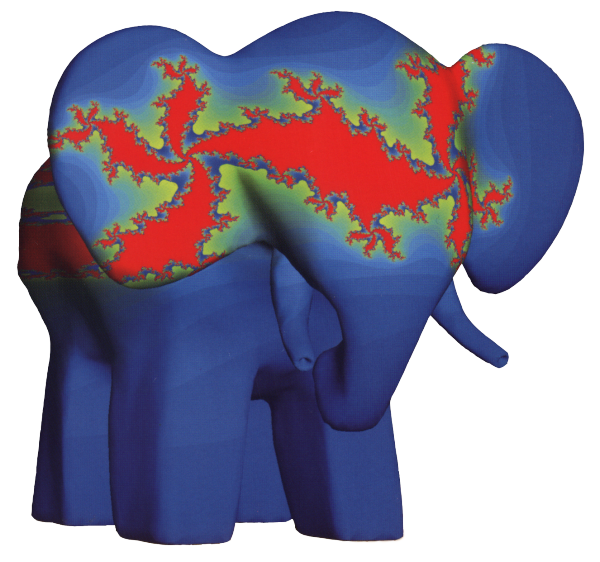
\includegraphics{images/sec-0/julia-elephant-s}
    \vspace*{1.87333708001in}	% height of julia-elephant-s

%    \hspace{0.5cm}
\includegraphics[height=1.87in]{images/misc/placeholder}
%    \vspace*{1.87in}
\end{minipage}}

\vspace{\stretch{2}}


%
% sec-i-disclaimer.tex
%

\pagebreak
\vspace*{\stretch{1}}
\noindent\makebox[0pt][l]{\begin{minipage}{\textwidth}
\flushleft
\begin{small}
    Cover art: Rost, Randi~J., OpenGL Shading Language, 2nd ed.\\
    (ISBN 0-321-33489-2)

    \vspace{4ex}
%
%    \emph{\project} copyright \copyright\ 2009, Trevor L. McDonell\\
%    Original Author: Trevor L. McDonell (trevor.mcdonell@gmail.com)

    Copyright \copyright\ 2009--2014, Trevor L.\ McDonell
\end{small}
\end{minipage}}

%
% sec-ii-declaration.tex
%

\pagebreak
\vspace*{1in}
\noindent\makebox[0pt][l]{\begin{minipage}{\textwidth}
    \centering
    This thesis is submitted in fulfilment\\
    of the requirements for the degree of\\[3ex]

    \textsc{\large Doctor of Philosophy}\\[3ex]

    School of Computer Science and Engineering\\
    %Faculty of Engineering\\[1.5ex]
    The University of New South Wales\\
    Australia

%    \textsc{\large Bachelor of Engineering (Mechatronics (Space))}\\[1.5ex]
%    \textsc{\large Bachelor of Engineering (Mechatronics / Space Engineering)}\\[1.5ex]
%
%    \emph{and}\\[1.5ex]
%
%    \textsc{\large Bachelor of Science (Advanced)}\\[3ex]
%
%    School of Aerospace, Mechanical\\
%    and Mechatronic Engineering\\[1.5ex]
%    University of Sydney\\
%    Australia
\end{minipage}}


\iftoggle{public}{%
  % nothing
}{%
  % Include signed statements of originality, copyright, and authenticity

\cleardoublepage
\vspace*{1in}
\subsubsection*{Originality Statement}

I hereby declare that this submission is my own work and to the best
of my knowledge it contains no materials previously published or written by
another person, or substantial proportions of material which have been accepted
for the award of any other degree or diploma at UNSW or any other educational
institution, except where due acknowledgement is made in the thesis. Any
contribution made to the research by others, with whom I have worked at UNSW or
elsewhere, is explicitly acknowledged in the thesis. I also declare that the
intellectual content of this thesis is the product of my own work, except to the
extent that assistance from others in the project's design and conception or in
style, presentation and linguistic expression is acknowledged.

\vspace{5mm}
\noindent\makebox[0pt][l]{\begin{minipage}{\textwidth}
    \centering
    \begin{tabular}[b]{cc}
      \iftoggle{public}{%
        \phantom{\framebox(228,57){}} &
        \phantom{\today}
      }{%
        \includegraphics{images/signature} &
        \today \hspace{8mm}
      }
    \end{tabular} \\
    \hfill{} \textsc{trevor lee mcdonell} \hfill{} \textsc{date} \hfill{}
\end{minipage}}


\cleardoublepage
\vspace*{1in}
\subsubsection*{Copyright Statement}

I hereby grant the University of New South Wales or its agents the right to
archive and to make available my thesis or dissertation in whole or part in the
University libraries in all forms of media, now and here after known, subject to
the provisions of the Copyright Act 1968. I retain all proprietary rights, such
as patent rights. I also retain the right to use in future works (such as
articles or books) all or part of this thesis or dissertation.

I also authorise University Microfilms to use the 350 word abstract of my thesis
in Dissertation Abstract International.

I have either used no substantial portions of copyright material in my thesis or
I have obtained permission to use copyright material; where permission has not
been granted I have applied/will apply for a partial restriction of the digital
copy of my thesis or dissertation.

\vspace{5mm}
\noindent\makebox[0pt][l]{\begin{minipage}{\textwidth}
    \centering
    \begin{tabular}[b]{cc}
      \iftoggle{public}{%
        \phantom{\framebox(228,57){}} &
        \phantom{\today}
      }{%
        \includegraphics{images/signature} &
        \today \hspace{8mm}
      }
    \end{tabular} \\
    \hfill{} \textsc{trevor lee mcdonell} \hfill{} \textsc{date} \hfill{}
\end{minipage}}


\cleardoublepage
\vspace*{1in}
\subsubsection*{Authenticity Statement}

I certify that the Library deposit digital copy is a direct equivalent
of the final officially approved version of my thesis. No emendation of content
has occurred and if there are any minor variations in formatting, they are the
result of the conversion to digital format.

\vspace{5mm}
\noindent\makebox[0pt][l]{\begin{minipage}{\textwidth}
    \centering
    \begin{tabular}[b]{cc}
      \iftoggle{public}{%
        \phantom{\framebox(228,57){}} &
        \phantom{\today}
      }{%
        \includegraphics{images/signature} &
        \today \hspace{8mm}
      }
    \end{tabular} \\
    \hfill{} \textsc{trevor lee mcdonell} \hfill{} \textsc{date} \hfill{}
\end{minipage}}

} % public



% Contents pages (only in book mode)
%
\cleardoublepage
\phantomsection
\addcontentsline{toc}{chapter}{Contents}
\tableofcontents\markboth{Contents}{Contents}

\cleardoublepage
\phantomsection
\renewcommand{\listfigurename}{Figures}
\addcontentsline{toc}{chapter}{\listfigurename}
\listoffigures\markboth{\listfigurename}{\listfigurename}

\cleardoublepage
\phantomsection
\addcontentsline{toc}{chapter}{\lstlistlistingname}
\lstlistoflistings\markboth{\lstlistlistingname}{\lstlistlistingname}
\addtocontents{lol}{\vspace{10pt}}

\cleardoublepage
\phantomsection
\renewcommand{\listtablename}{Tables}
\addcontentsline{toc}{chapter}{\listtablename}
\listoftables\markboth{\listtablename}{\listtablename}


\chapter{Abstract}
\markboth{Abstract}{}

Computers are no longer getting faster. Instead, including multiple cores on a
single chip has become the dominant mechanism for scaling processor performance,
and the exponential growth in the number of cores on a single processor is
expected to lead in a short time to mainstream computers containing hundreds of
devices. Unfortunately, programming parallel computers is known to be an
extremely challenging task, even for expert computer programmers.

In order to achieve improved single-application performance on such processors,
an appropriate programming model is needed which can expose parallelism and
address scalability. Commodity graphics processing units, which have evolved
into flexible general-purpose parallel architectures, can provide some insight
into many of the challengers developers will face; finding parallelism within
our applications to satiate available hardware, and rationalising the
interactions of large numbers of concurrent threads.

This thesis presents the design, implementation, and evaluation of a new
domain--specific language embedded within Haskell for flat data-parallel array
computations executed on graphics processing units. The design concentrates on
providing a high--level abstraction that composes computations that run
efficiently according to the strengths and weaknesses of the underlying
hardware, without forcing the programmer to recast their algorithm to fit within
that architecture.

The main contribution of this thesis is an embedded language \emph{Accelerate},
which is more expressive than previous languages targeting general purpose
computations on graphics processors, while benchmarks show that programs in
Accelerate can be competitive with those written in traditional lower-level
languages. Through the work done in this thesis, Accelerate has become the
dominant method for GPGPU programming in Haskell.


%          File: sec-iv-acknowledgements.tex
%       Created: Sat 07 Oct 2006 03:11:37 PM EST
% Last Modified: Mon 23 Oct 2006 12:03:27 PM EST

\chapter{Acknowledgements}
\markboth{Acknowledgements}{}

\begin{center}

My supervisors Manuel and Gabi, for their (usually) gentle guidance, and for
allowing me the opportunity and (most importantly) the time to explore possibilities.
\\\qquad

My friends and family, for putting up with me when things got out of hand\\
(as they inevitably do).
\\\qquad

And of course, to Josephine, for her unwavering support and encouragement.

\end{center}



% MAIN MATTER
% ~~~~~~~~~~~

\mainmatter
\fancyhead[ER]{\small\textsc{\chaptername\ \thechapter}}
\fancyhead[OL]{\small\textsc{\sectionname\ \thesection}}

% Add chapter thumbs for the main matter section only. At the beginning of the
% back matter we stop displaying thumbs and revert to \oldchapter
%
\let\oldchapter\chapter
\renewcommand{\chapter}[1]{\oldchapter{#1}\addthumb{#1}{}{white}{black}}


\chapter{Introduction}
\label{ch:introduction}

\epigraph{%
Unless someone like you cares a whole awful lot,\\
nothing is going to get better. It's not.}%
{\textsc{---dr. seuss}\\\textit{The Lorax}}

% \epigraph{I hear you say ``Why?'' Always ``Why?'' You see things; and you say, ``Why?''\\
% But I dream things that never were; and I say, ``Why not?''}%
% {\textsc{---george bernard shaw}\\\textit{Back To Methuselah}}

% \epigraph{First things first, but not necessarily in that order.}
% {\textsc{---the doctor}}

%\epigraph{Come then, and let us pass a leisure hour in
%storytelling,\\and our story shall be the education of our heroes.}%
%{\textsc{---plato}\\\textit{Republic}, \textsc{book ii}}

The beginning of the twenty first century has seen an interesting trend in
computing emerge. General purpose CPUs, such as those provided by Intel, IBM and
AMD, have increased performance substantially, but with nowhere near the
increases seen in the late 1980's and early 1990's. To a large extent, single
threaded performance increases have tapered off, due to the low level of
inter-process communication in general purpose workloads, and the physical
limitations of power dissipation for integrated circuits. The additional
millions and billions of transistors afforded by Moore's rule\footnote{Moore's
actual prediction in 1965 referred only to the number of devices that could be
fabricated on a single die, and that this quantity would increase by fifty
percent each year \cite{Moore:1965wc}. I refrain from using the commonly held
name of ``Moore's Law'' as this trend is not a law in the sense defined by the
physical sciences, such as the Laws of Gravity and Thermodynamics --- it is
simply a description of observed facts, rather than a principle driven by some
fundamental controlling influence.} are simply not very productive in increasing
the performance of single--threaded code.

At the same time, the commodity \emph{graphics processing unit} (GPU)\gpu{} has
been able to use this ever increasing transistor budget effectively,
geometrically increasing rendering performance, as \indext{rasterisation} is
an inherently parallel operation.
%
% Historically fixed function pipelines, graphics architectures are
% evolving to become increasingly flexible as well as powerful, consisting of an
% expressive set of general purpose computation resources, with some fixed
% function units for graphics operations on the side.
%
Modern GPUs are massively parallel multicore processors, offering instruction
throughput and memory bandwidth rates much higher than those found on
traditional CPUs~\cite{NVIDIA:2012wf}. However, despite the advertised potential
of $100\times$ speedups, development of high-performance \emph{general-purpose
GPU} (GPGPU)\gpgpu{} programs requires highly idiomatic programs, whose
development is work intensive and requires a substantial degree of expert
knowledge.

Several researchers have proposed methods to ameliorate the status quo by either
using a library to compose GPU\gpu{} code or by compiling a subset of a
high-level language to low-level GPU
code~\cite{McCool:2004,Bond:2010bd,ThrustAParallelT:ub,Catanzaro:2011cn,Mainland:2010vj,CLyther:EvXSiruK,Muranushi:2012eh}.
This thesis is in the same spirit: we propose a domain-specific high-level
language of array computations, called \emph{Accelerate}, that captures
appropriate GPGPU\gpgpu{} programming idioms in the form of parameterised,
collective array operations. Our choice of operations was informed primarily by
the \emph{scan-vector model}~\cite{Chatterjee:1990vj}, which is suitable for a
wide range of algorithms and can be efficiently implemented on modern
GPUs~\cite{Sengupta:2007tc}.

The beginning of the Accelerate project predates this thesis, and several
researchers have contributed to it in that time. The following summarises the
main areas I have contributed to, and I have explicitly noted which are my own
individual work:
%
\begin{itemize}
    \item We have developed an embedded language, \emph{Accelerate}, of
        parameterised collective array computations that is more expressive than
        previous GPGPU\gpgpu{} proposals (Section~\ref{sec:accelerate}).

    \item I implement a dynamic code generator based on CUDA\cuda{}
        skeletons\skeleton{} of collective array operations that are
        instantiated at runtime (Sections \ref{sec:code_generation} \&
        \ref{sec:instantiating_skeletons}).

    \item I implement an execution engine that caches previously compiled
        skeleton instances and host-to-device data transfers, as well as
        parallelises code generation, data transfer, and GPU\gpu{} kernel
        loading, configuration, and execution
        (Sections~\ref{sec:dynamic_compilation},
        \ref{sec:memory_management}, \&
        \ref{sec:executing_programs}).

    \item We introduce a novel sharing recovery algorithm for type-safe abstract
        syntax trees, preserving the structure of the deeply embedded program
        (Section~\ref{sec:sharing_recovery}).

    \item I introduce type preserving optimisations of embedded language array
        programs, including a novel approach to array fusion
        % as well as scalar simplifications
        (Sections~\ref{sec:manipulating_embedded_programs},
        \ref{sec:array_fusion}, \&
        \ref{sec:simplification}).

    \item Benchmarks assessing runtime code generation overheads and kernel
        performance for a range of programs (Chapter~\ref{ch:results}).
\end{itemize}

Although we motivate and evaluate our work in the context of the Accelerate
language, our contributions are not limited to this context. Specifically, our
sharing recovery algorithm applies to any embedded language based on the typed
lambda calculus, and my approach to array fusion applies to any dynamic compiler
targeting bulk-parallel SIMD hardware. The current implementation targets
CUDA\cuda{}, but the same approach works for OpenCL, as well as traditional CPU
programming languages such as C and LLVM.

Our results show that Accelerate programs can be competitive with programs
hand-written in CUDA\cuda{}, while having a much higher level of abstraction.
Because of the work undertaken in this thesis, we have seen Accelerate gain
traction within academia and industry, including:

\begin{itemize}
    \item Simon Marlow has recently published a book on \emph{Parallel and
        Concurrent Programming in Haskell}~\cite{Marlow:2013wn}, which includes
        a chapter on GPU programming using Accelerate.

    \item Peter Braam of Parallel Scientific is building a high level DSL in
        Haskell based on Accelerate, for image reconstruction computations for
        the Square Kilometer Array, the largest radio telescope in the world.

    \item Andy Gill has recently been awarded an NSF grant to research
        resource-aware DSLs for high performance computing applications, and is
        building on top of Accelerate.\footnote{\url{http://www.nsf.gov/awardsearch/showAward?AWD_ID=1350901}}

    \item Flowbox\footnote{\url{http://www.flowbox.io}} is a startup developing
        tools for composition and visual effects for images and video that is
        built on top of Accelerate. Flowbox is generating interest amongst
        several Hollywood studios as a promising new technology.

%    \item Matt Sottile of Galois is using Accelerate for computations in a
%        research project that attempts to reconstruct the brain activity of a
%        simple worm.

    \item We commonly see research papers on array-based computations and
        languages, particularly in a functional programming context, include a
        comparison to Accelerate in their own benchmarks.\footnote{However, I
        modestly refrain from going so far as to claim that my work in this
        thesis has set a new standard by which functional array-based
        programming languages are measured.}

\end{itemize}

We will discuss related work as each topic arises. The source code for
Accelerate including all benchmark code is available from
\url{https://github.com/AccelerateHS}.


% Parallel programming models fall into two broad categories. Task parallelism
% emphasises a distributed model for independent processes, whereas data
% parallelism specifies a single computation which is applied simultaneously
% across a large number of data elements. While task parallelism typically does not
% scale well with the size of the problem, data parallelism provides one of the
% most promising approaches to making efficient use of parallel hardware.
%
% Despite their attractiveness for computationally intensive operations, accessing
% this performance has remained elusive for all but a few applications. The
% arithmetic power of the GPU is a result of a highly specialised and constrained
% architecture, resulting in programs which rely heavily on the CPU to handle
% difficult parts of control and data flow. However, the CPU--GPU link is
% relatively slow, engendering high communication latencies which radically impair
% performance. To be practicable, the GPU programming model must efficiently
% support messy boundary conditions, irregular data and control flow patterns, and
% provide an elegant mapping from the application to the underling architecture,
% without forcing the programmer to recast their algorithm. Support for nested
% data parallelism \cite{Blelloch:1994vc,Blelloch:1996jx} (NDP) would provide a
% first step towards a viable GPU programming model, unshackling vast
% computational resources from the small application niche for which they were
% originally designed.


% %
% Background / Literature Review
%
% The literature review is an organisational pattern that combines both summary
% and synthesis. It may give a new interpretation of old material, combine old
% and new interpretations, or trace the intellectual progression of a field. It
% should be organised around ideas, not expand each source individually.
%
% - What themes and issues connect the sources together?
% - What solutions are present, which aspects are missing?
% - What is the trend in the field?
%
% http://blog.accelereyes.com/blog/2013/03/07/cpu-processing-trends-for-dummies/
%

\chapter{Background}
\epigraph{Why waste time learning, when ignorance is instantaneous?}
{\textsc{---calvin and hobbes}}
\label{ch:background}

%
% Progression:
%  1. Technology trends, move towards increasing parallelism
%  2. Parallel computing, introduce NDP and speedup/code -> inf promise
%  3. GPGPU. Short history. Problems, need for reuse, abstraction from HW
%  4. Develop a need/motivation to combine (2) and (3)
%
% Organisation:
%  1. Introduction: quick idea of the topic, central theme
%  2. Body: sources thematically
%  3. Conclusion and recommendations
%
%  + Models and Languages for Parallel Computing
%    + Challenges to Parallel Computing
%    + Approaches to Parallel Computing
%    + Evaluating Parallel Programs
%
%  + Parallel Programming for Graphics Processing Units
%  + CUDA
%    + Hardware Model
%    + Programming Model
%    + Execution Control
%    + Memory Model
%
%  + Motivation
%

MMTC: Chapter 2 (Background): Don't bother introducing Haskell and things like parallelism vs concurrency etc. What you need to discuss is (1) data parallelism and (2) how GPGPU programming is data parallel programming. Then, (3) the idea of embedded languages and runtime code generation. However, don't go into too much details at this point. After all, much of this has been discussed in existing literature already. I'd suggest to pick 1-2 examples and use them to drive the explanations (and at the same time give people an idea for the feel of Accelerate programs).


\begin{itemize}
\item Functional programming (3 days)
    \begin{itemize}
        \item Basic Haskell introduction
        \item bulk programming style, function composition
        %\item denotional semantics?
    \end{itemize}

\item Parallel programming (1 week)
    \begin{itemize}
        \item parallel vs. concurrent (1 day)
        \item data parallelism; examples (2 days)
        \item evaluating parallel programs (3 days)
            \begin{itemize}
                \item work and depth complexity
                \item parallel speedup
                \item wall clock time
                \item instruction vs. bandwidth limited programs
            \end{itemize}
    \end{itemize}

\item Parallel programming with CUDA (2 weeks)
    \begin{itemize}
        \item GPGPU programming (3 days)
            \begin{itemize}
                \item why bother?
                \item performance vs. development time
            \end{itemize}
        \item CUDA programming model (1.5 weeks)
            \begin{itemize}
                \item programming model, SIMD architecture
                \item execution model: kernels, warps, thread blocks
                \item memory model, coalescing
                \item execution control (host/device)
            \end{itemize}
    \end{itemize}

\item Embedded languages (1.5 weeks)
    \begin{itemize}
        \item dis/advantages: using tools/features of host language; recreating
            functionality of the host compiler (optimisations)
        \item deep (Accelerate) vs. shallow (Repa) embeddings
            % \url{http://skillsmatter.com/podcast/scala/making-edsls-fly}
        \item DSLs in Haskell (1 week)
            \begin{itemize}
                \item simple (untyped) DSL
                \item GADTs to encode type safety / invariants
                \item type-safe evaluator
                \item itemize design requirements / goals of this language
            \end{itemize}
    \end{itemize}
\end{itemize}



Modern microprocessor technology is constructed from millions of interconnected
switching devices, called transistors. As process technology advances, these
transistors, and the interconnections between them, can be fabricated in a
smaller area. The challenge for microprocessor architects is to translate this
increase in resources into an increase in performance.

Unfortunately, computers are no longer getting faster. Instead, we are being
offered computers containing more and more CPUs, each of which is individually
not substantially faster than those of the previous generation. As the number of
processors increases, it will become increasingly important for programmers to
utilise these additional processing elements.

Processor designs are clearly evolving in one direction: towards massive
parallelism and many-core architectures. Unfortunately, the model of programming
used in mainstream languages was developed many years ago, when programs were
sequential and architectures were relatively simple. As hardware architectures
become larger and more complex, these traditional low-level approaches to
parallel programming become less and less tractable for real applications.

This section \ldots


\section{Parallel Programming}

Programming parallel computers is an extremely challenging task. This is true
even for expert computer programmers, let alone for scientists in other
disciplines whose computations are often what drive the acquisition of
high-performance machines. For many years, parallel computing has waned in and
out of favour, alternatively seen as the solution to all computational
limitations or a waste of time, given the rate at which processor and memory
speeds improve. These changing perceptions are the result of many factors,
including the programming environments available to users, the types of
supercomputing hardware on offer from vendors, and continual changes in the
focus of the academic community as to what are the ``hot'' problems of the time.

Nevertheless, the promise of parallel computing remains the same today as it was
at its inception. If users can buy sequential computers with gigabytes of
memory, imagine how much faster their programs could run if \emph{p} of these
machines were working cooperatively; imagine how much larger a problem could be
solved if the memories of these \emph{p} machines were used collectively.

The challenges to realising this potential faces two main difficulties; the
hardware, and the software. The former asks ``how do I build a parallel computer
that will allow these \emph{p} processors and memories to cooperate
efficiently?'' Then, given such a platform the latter asks ``how do I express my
computation such that it will utilise these \emph{p} processors and memories
effectively?''

In recent years there has been a growing awareness that while the parallel
computing community can build machines that are reasonably efficient and
affordable, the population of users that can effectively program these machines
comprises only a small fraction of those who can program traditional sequential
computers. Moreover, even the best parallel programmers can not do so without
significant effort. Parallel programming is still seen by many as an arcane
skill, a black art; best avoided if possible.

However, recent changes to the landscape of computing hardware will likely force
even mainstream application developers to abandon the ways of sequential
programming. In order to continually increase performance, compiler and
processor designers have struggled to to automatically exploit the implicit
parallelism present in serial programs. Using this technique, instructions can
be rescheduled in order to best exploit the multiple functional units available
in superscalar architectures. However, experience has shown that most serial
programs contain limited implicit parallelism \cite{Wall:1991}. While
techniques exist that can raise this limit somewhat, they come at the cost of
increased power to performance ratios and hardware complexity. Automatic
extraction of parallelism without explicit assistance from the programmer has
reached the point of diminishing returns. Including multiple cores on a single
chip has now become the dominant mechanism for scaling processor performance,
and there is renewed interest in parallel programming models, languages and
platforms.

At the same time, one must concede that programming a parallel machine is
inherently more difficult than sequential programming, as programmers must think
not only of correctness but concurrency and communication as well. It
undoubtedly complicates a programmer's life, but there is no silver bullet.
However, a good programming model should be able to unburden the programmer from
dealing with trivia, automating the more tedious aspects of mapping the
computation to the target hardware. Ideally, the programmer should focus on
%making major policy decisions and on
designing a correct and efficient algorithm.


\section{Haskell}
%
% Possible; Haskell compared to:
%   + static languages
%   + dynamic languages
%

\indexe{Haskell} is a general-purpose \emph{purely functional programming
language} with \emph{non-strict semantics} \index{non-strict semantics|see{lazy}}
and \emph{strong static typing}\index{typing!static}. In an imperative programming
language you get things done by giving the computer a sequence of actions to
perform and letting it execute them. While executing these statements the
computer is typically allowed to change some state: setting some variable
\texttt{ans} to $42$, doing some stuff, and then changing \texttt{ans} to
something else. In contrast, purely functional programming is not so much
concerned with telling the computer what to \emph{do} in so much as telling it
what stuff \emph{is}. The factorial of a number is the product of all the
numbers from one to that number; the sum of a list of numbers is the first
number plus the sum of the rest of the numbers; and so on. This is expressed in
the form of \emph{functions}, and programs can then be thought of as a sequence
of functions applying a series of transformations on data.

Haskell is a \indexe{pure} language; if you say some variable \texttt{ans} has
the value $42$, you can not later say that it has a different value. We assert
that pure functions like this do not have any \indexe{side effects}: the only
thing they can do is to perform some calculation on their inputs and return a
result. This might at first seem limiting, but has a rather nice consequence: if
a function is called twice with the same inputs, it will always return the same
result. This is known as \indexe{referential transparency} and not only allows
the compiler to reason about the behaviour of the program, but also allows the
user to deduce the \indexe{correctness} of a function and to build complex
functions by gluing together simpler functions.

Haskell is a \emph{statically typed}\index{typing!static} language; when you
compile your program the compiler knows which piece of code is a number, which
is a string, and so on. As such many possible errors are caught at compilation
time; the compiler will complain if you attempt to add a number to a string, for
example. Haskell uses a very good system of type inference based on
Hindley--Milner \textcolor{blue}{[citation needed]}, so that you don't have to
explicitly label each piece of code with a type.

Haskell is a \indexe{lazy} language; unless told otherwise it will not
explicitly evaluate functions or calculate values until a result is actually
required. Lazy evaluation might seem to have some spooky effects, but goes in
hand with the idea of referential transparency and profoundly affects how one
writes programs.

While Haskell encourages the pure, lazy style of functional program, this is
merely the default option. Haskell supports stateful functions, using distinct
types for functions with side effects orthogonal to the type of pure functions,
ensuring the two can not be conflated. While the focus of the language is
writing statically typed programs it is possible, although rare, to write
dynamically typed programs as well.


% \subsection{Syntax}
% basic crash course necessary?

% \subsection{Style}


\section{CUDA}


%
% sec-3-design.tex
%
% Embedded languages, stratified types, richly typed terms, representing
% programs. The Accelerate language.
%
% Accelerate CUDA backend. Code generation. Executing computations. Garbage
% collection. Caching.
%

% Need a better title
\chapter{Basics}  % Design of an embedded language
\epigraph{You see a wile, you thwart. Am I right?}%
{\textsc{---terry pratchett and neil gaiman}\\\textit{Good Omens}}


\section{Data Parallelism}
\label{sec:data_parallelism}

The major processor manufacturers and architectures have long since run out of
room with most of the traditional approaches to boosting CPU performance.
Instead of driving clock speed and straight-line instruction throughput,
including multiple cores on a single chip has become the dominant mechanism for
scaling processor performance. Despite this trend being apparent for a number of
years, programming parallel computers remains an extremely challenging task ---
even for expert computer programmers, let alone for scientists in other
disciplines.

One programming model that has shown to make good use of parallel hardware is
\indexe{data parallelism}.
% The idea is that the application of an operation over
% a collection of data, such as an array, can often be performed in parallel.
Data parallelism focuses on distributing the data over the available processors,
and for each processor to perform the \emph{same} task on the \emph{different}
pieces of distributed data. To the programmer, data parallelism exposes a single
logical thread of execution that is fairly easy to understand and reason about.
In addition to its simplicity, the data parallel approach to programming
parallel computers has several advantages:
%
\begin{enumerate}
\item The model is independent of the number of processors, so scales to any
    number of processors by decomposing data into the appropriate number of
    chunks.

\item All synchronisation is implicit, so the programming model is safe from
    race conditions, eliminating a major source of errors in parallel programs.

\item As memory bandwidth is often a limiting factor in modern computers, the
    emphasis on data layout can assist with both data flow as well as
    parallelisation.
\end{enumerate}
%
In the world of massively parallel computing with strong locality requirements,
data parallelism is the well established, demonstrably successful brand leader.
Examples of data parallel programming environments include High Performance
Fortran (HPF)~\cite{HPF:1997}, the collective operations of the Message Passing
Interface (MPI)~\cite{MPI:2012}, Google's Map/Reduce
framework~\cite{Dean:2008fi}, and NVIDIA's CUDA API for graphics
processors~\cite{NVIDIA:2012wf}.


\section{GPU computing} % {GPGPU programming is data parallel programming}
\label{sec:gpu_computing}

General-purpose computing on graphics processing units
(\indext{GPGPU}\index{GPGPU|see {general-purpose computing on graphics
processing units}}) is the utilisation of a graphics processing unit (\GPU),
which typically handles the computations for computer graphics, to perform
computations in applications typically handled by the central processing unit
(CPU). Since general purpose CPUs are designed to optimise the performance of a
single thread of execution, much of the processor's resources (die area and
power) to non-computational tasks such as caching and branch prediction.
Conversely, the highly parallel nature of graphics processing (rasterisation)
means the GPU architecture instead uses these resources to be able to execute
many tasks in parallel, improving the computational throughput for parallel
workloads at the expense of decreased single threaded performance. This
difference in architectures between the CPU and GPU is illustrated in
Figure~\ref{fig:cpu_gpu_block_diagram}.

\begin{figure}[tbp]
    \centering
    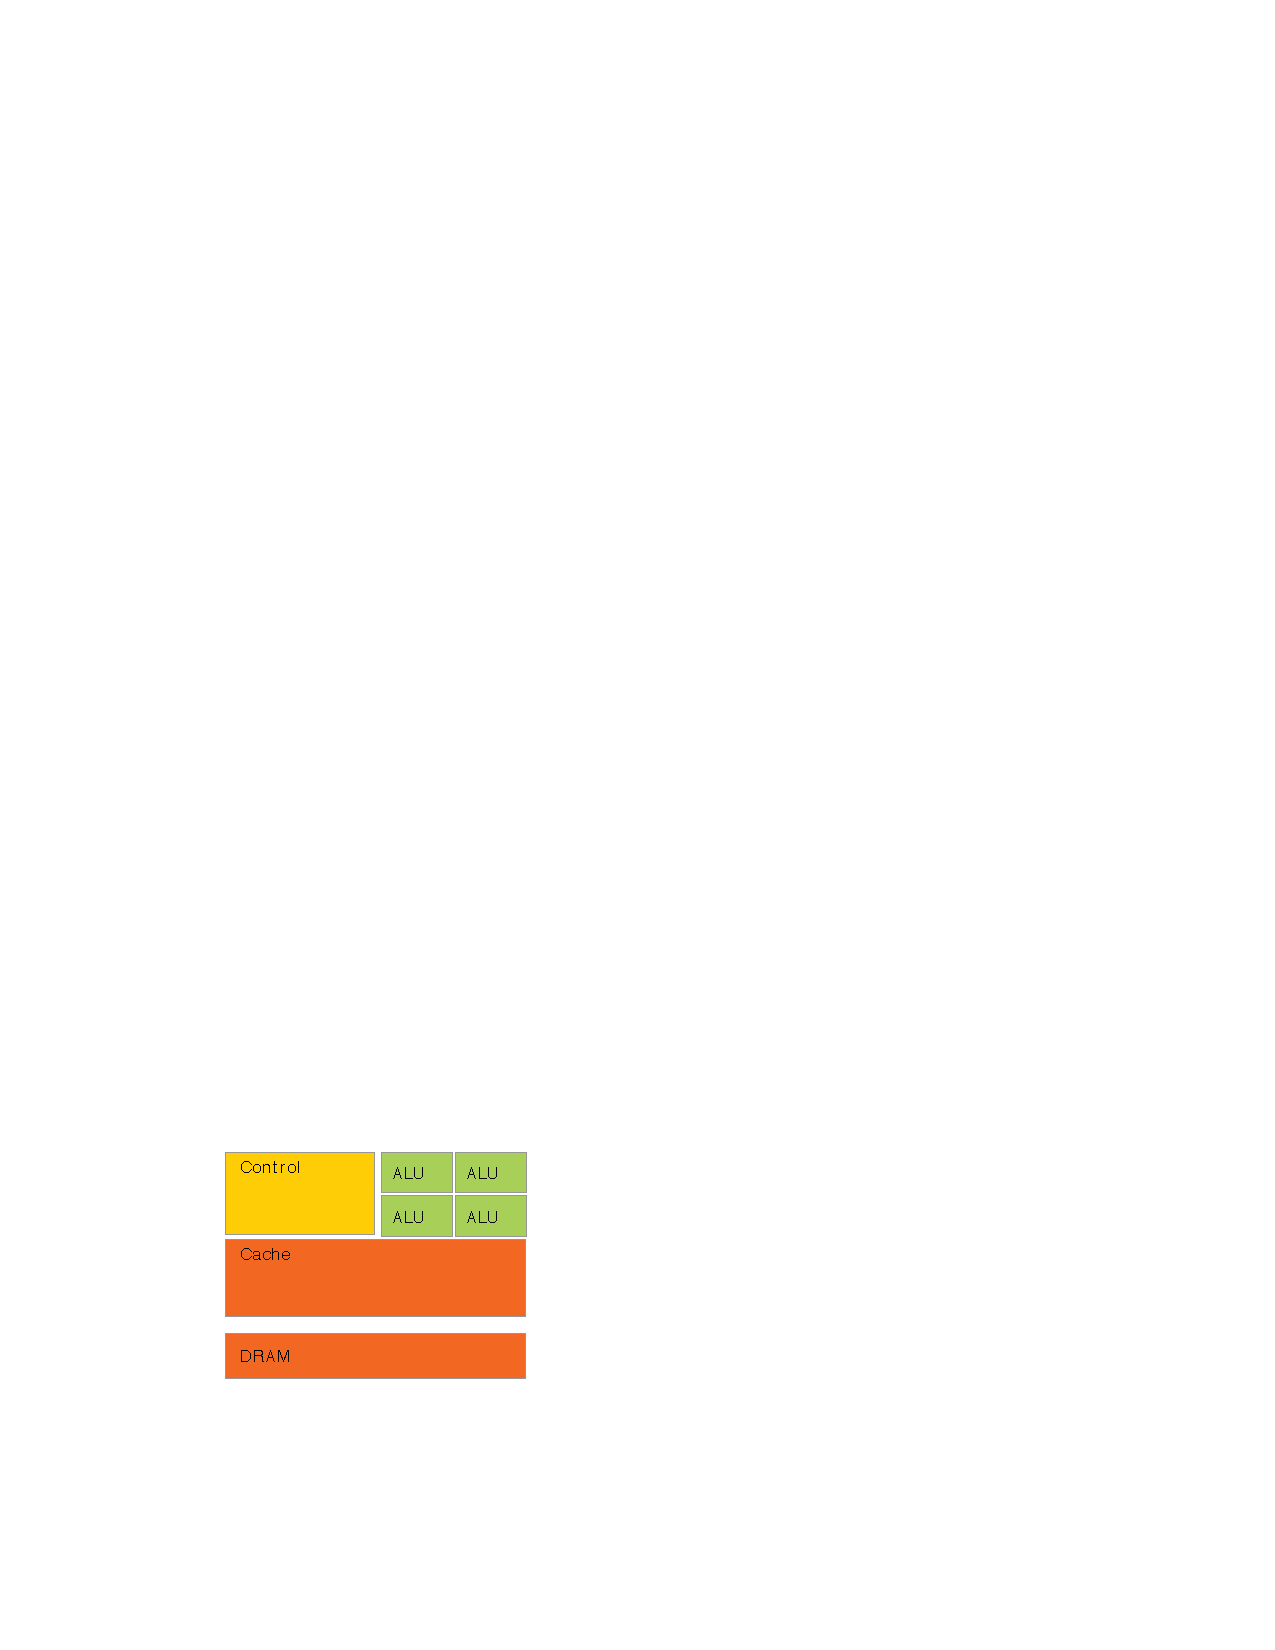
\includegraphics[width=0.4\textwidth]{images/sec-3/block_cpu}
    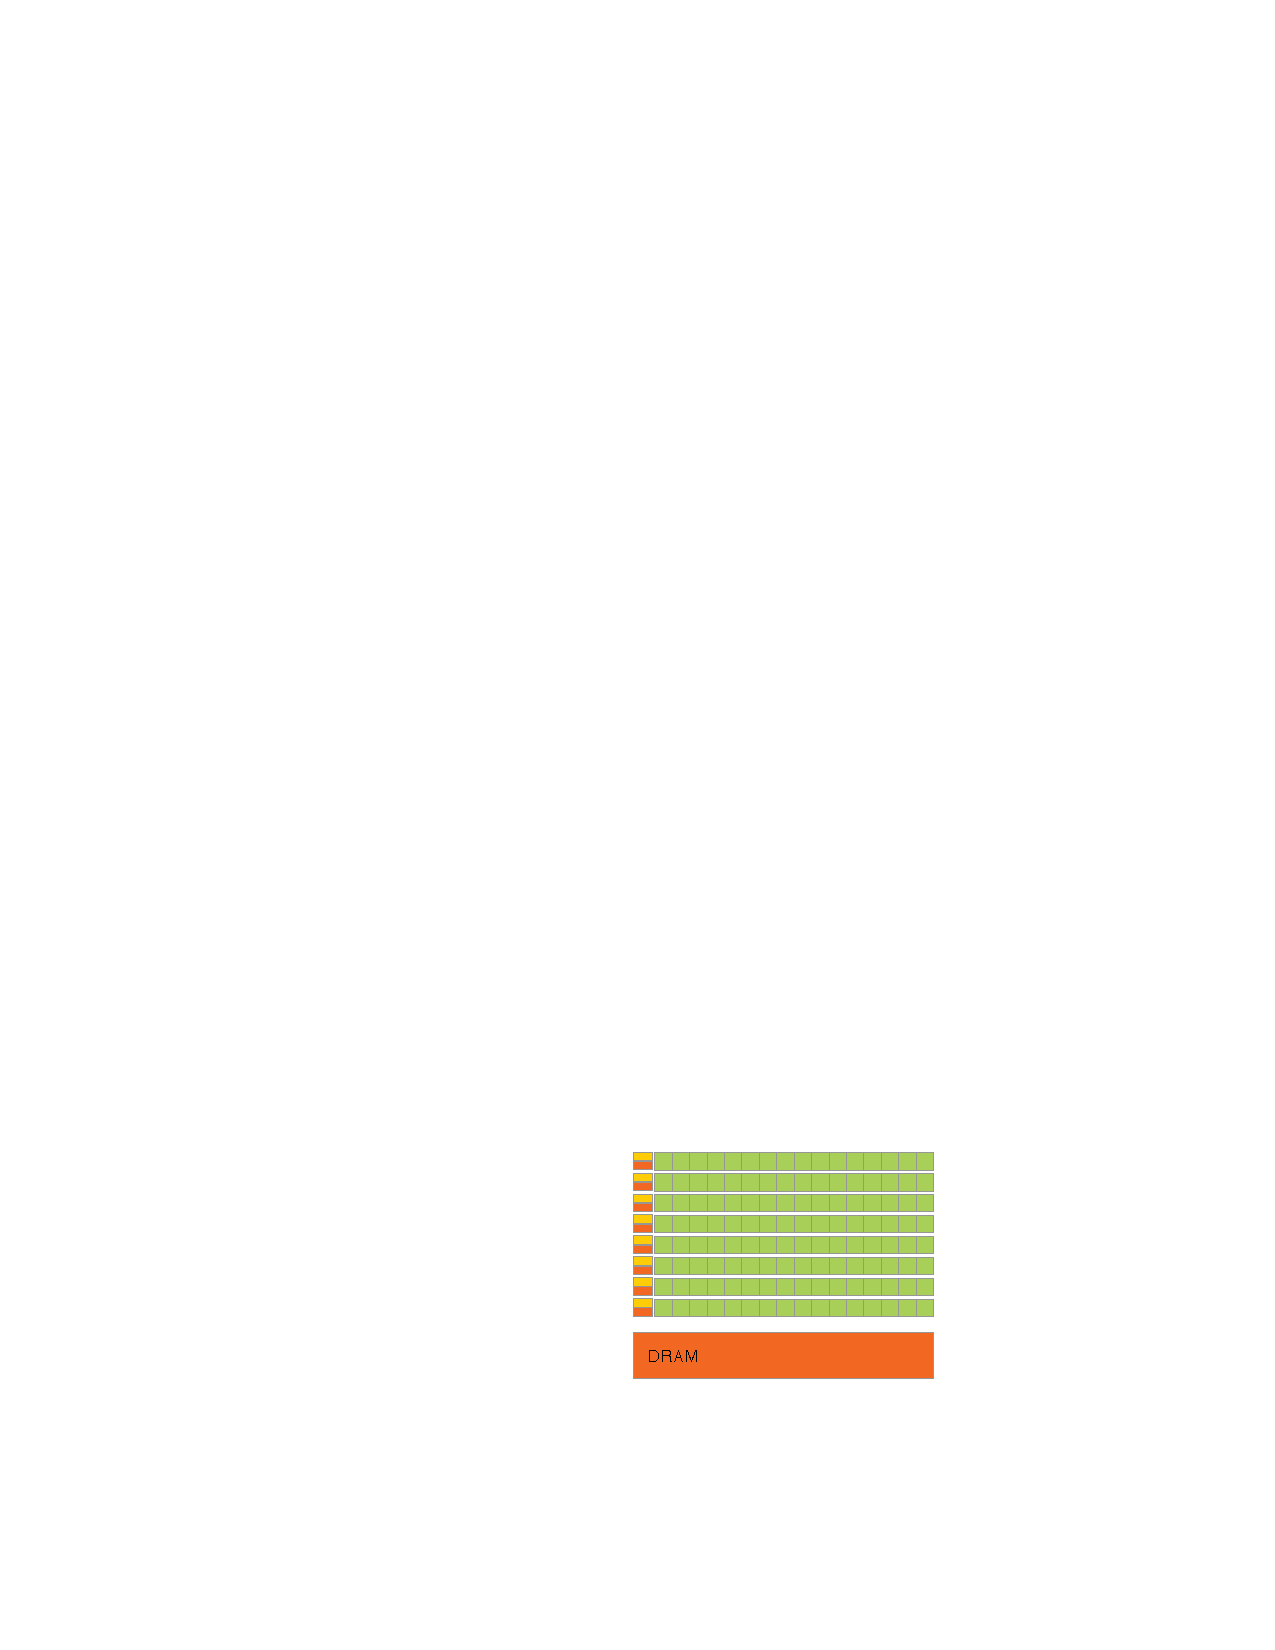
\includegraphics[width=0.4\textwidth]{images/sec-3/block_gpu}
    \caption[The GPU devotes more transistors to data processing]{Block diagram
    comparing the relative use of transistors in a CPU (left) compared to a GPU
    (right). The GPU is specialised for highly parallel, compute intensive
    workloads, and so is designed such that the majority of its transistors are
    devoted to data processing, rather than data caching and control flow.
    Images from~\cite{NVIDIA:2012wf}.}
    \label{fig:cpu_gpu_block_diagram}
\end{figure}

More specifically, the GPU is especially well suited to expressing problems that
can be expressed as data parallel computations, where the same program is
executed by many processors on many different data elements in parallel
(\S\ref{sec:data_parallelism}). Because the same program is executed by many
processors, there is no need for sophisticated control flow, and because it is
executed on many data elements, memory access latency can be hidden with
calculations rather than by big caches. Many applications that process large
data sets can use the data parallel programming model to speed up calculations,
and these applications can be coded to execute on the GPU.


\subsection{CUDA}
\label{sec:cuda}

\CUDA is the parallel computing platform and programming model created by
NVIDIA, which gives programmers direct access to the memory and parallel
computation units of their GPUs. Using CUDA, the massively parallel multicore
architecture of the GPU becomes accessible for general purpose computing, not
just graphics.

CUDA extends the C programming language by allowing the C programmer to define
functions, called \emph{kernels}\index{GPU!kernel}, that, when called, are
executed $n$ times in $n$ data parallel threads on the available processing
elements, rather than only once like regular C functions. These functions are
executed by threads arranged in a multidimensional structure of \emph{thread
blocks}\index{GPU!thread block}. Threads within a block can cooperate by sharing
data through some \emph{shared memory}\index{GPU!shared memory} and by
synchronising their execution to coordinate memory access. More precisely, the
programmer can specify synchronisation points in the kernel by calling
@__syncthreads()@\index{GPU!\code{__syncthreads()}}, which acts as a barrier at
which all threads in the block must wait before any is allowed to proceed. Each
thread block executes independently of each other, so a GPU with a higher number
of CUDA cores --- or \emph{streaming multiprocessors}\index{GPU!streaming
multiprocessor} (SM) --- will execute the program in less time than a GPU with
fewer multiprocessors.

\begin{lstlisting}[style=cuda
    ,float
    ,label=lst:cuda_vecadd
    ,caption={[CUDA kernel for pair wise addition of two vectors]A CUDA kernel
        that illustrates pair wise addition of two vectors. The
        \code{__global__} keyword marks a function as a kernel that should be
        executed on the GPU in data parallel. The execution configuration syntax
        \code{<<<...>>>} specifies the number of threads that will each execute
        the function in data parallel.}]
// Kernel definition
__global__ void VecAdd(float *A, float *B, float *C, int N)
{
    int i = blockIdx.x * blockDim.x + threadIdx.x;

    if (i < N) {
        C[i]  = A[i] + B[i];
    }
}

int main()
{
    ...
    // Kernel invocation with N threads
    int threadsPerBlock = 128;
    int numBlocks       = (N + threadsPerBlock - 1) / threadsPerBlock;
    VecAdd<<<numBlocks, threadsPerBlock>>>(A, B, C, N);
    ...
}
\end{lstlisting}

At an example, Listing~\ref{lst:cuda_vecadd} illustrates the pair wise addition
of two vectors $A$ and $B$ of size $N$ each, and stores the result in a vector
$C$. The kernel is defined with the @__global__@ declaration specifier. The
number of CUDA thread blocks and the number of threads in each block that
execute the kernel, at this invocation, is specified in the @<<<...>>>@ syntax.
Moreover, Listing~\ref{lst:cuda_vecadd} demonstrates that the GPU programming
model as exposed by CUDA is a data parallel programming model --- $N$ threads
execute $N$ individual instances of the kernel function @VecAdd@, and each
thread operates on a single element of each input array to create a single value
in the result.


\section{Embedded domain-specific languages}
\label{sec:EDSLs}

A \indexe{domain-specific language} (DSL) is a computer language specialised to
a specific problem domain. The DOT language~\cite{Graphviz:1998ui,Ellson:2001wf}
is an example of a DSL for describing graphs. This is in contrast to a general
purpose language such as Haskell~\cite{Haskell:1998}, which is broadly
applicable across domains but may lack specialised features for a particular
domain. A domain specific language is created to solve problems in a particular
domain, and is not intended to solve problems outside it (although this may be
technically possible). Restricting the problem domain the language is intended
to solve may allow for more optimisations during compilation, or increased
expressivity when representing problems or defining solutions in that domain.

An \emph{embedded} (or \emph{internal}) \emph{domain-specific
language}\index{domain-specific language!embedded} (EDSL) is a domain-specific
language that is designed to be used from within another host
language~\cite{Hudak:1996}. The embedded language is implemented as a library,
so is able to reuse the syntax and features of the general purpose host language
compiler, including compilation phases such as lexing, parsing, and semantic
analyses such as type checking, while adding domain specific elements such as
data types, or domain specific optimisations and code generation.

There are two major degrees in which an embedded language can be implemented:

\subsection{Shallow embedding}

In a shallow embedding, operations in the embedded language translate directly
into operations in the target language. A shallow embedding captures the
semantics of the data of the domain in a data type, and provides a \emph{fixed}
interpretation of that data. Thus, it is easy to add new constructs to the
language --- so long as they can be interpreted in the semantic domain --- and
the embedded language can reuse features of the host language, such as variable
binding.


\subsection{Deep embedding}

A deep embedding captures the semantics of the embedding by reflecting the
operations of the object language into a data structure. This data structure ---
an \indexe{abstract syntax tree} (AST) --- then permits transformations, such as
optimisations, before being translated into the target language. Deeply embedded
languages therefore enable a \emph{variable} interpretation of operations in the
domain, so it is easy to add new interpretations of the embedding, for example,
compiling to a different target language. However, adding new language
constructs requires extending the AST data type, and the implementation must
deal explicitly with binding of variables. Sharing and recursion are common
problems when implementing deeply embedded languages.

As the deeply embedded language runs inside of the host language, reflecting
operations into an AST, an interpreter for the embedded language must be
embedded within the host application.
% This interpreter may execute instructions in the internal language directly,
% or it may generate code that is compiled into machine language instructions to
% be executed.
As the interpreter executes code for the embedded language at program runtime,
code in the embedded language may either be written by the user or generated
dynamically by the application. If the target language is different to that of
the host language, this entails the interpreter generating, compiling, and
executing code for the target language at program runtime.


\section{The Accelerate EDSL}

The current generation of graphical processing units (GPUs) are massively
multicore processors (\S\ref{sec:gpu_computing}). They are optimised for
workloads with a large degree of data parallelism (\S\ref{sec:data_parallelism})
and good performance depends on highly idiomatic programs with low SIMD
divergence and regular memory-access patterns. Hence, the development of
applications that use the graphics processors for general purpose computations
(\S\ref{sec:gpu_computing}) is work intensive and requires a substantial degree
of expert knowledge.

Accelerate is our approach to reducing the complexity of GPU programming: a
high-level, deeply embedded domain-specific language (\S\ref{sec:EDSLs}) of
array computations that captures appropriate GPGPU idioms in the form of
parameterised, \indexe{rank-polymorphic}~\cite{Keller:2010er}, collective
operations on arrays~\cite{Chakravarty:2011fr}. Our choice of operations was
informed by the \emph{scan-vector model}~\cite{Chatterjee:1990vj}, which is
suitable for a wide range of algorithms, and demonstrated that these operations
can be efficiently implemented on modern GPUs~\cite{Sengupta:2007tc}.

We regard Accelerate's collective array operations as algorithmic
skeletons~(\S\ref{sec:code_generation}) that capture appropriate GPU programming
idioms. The dynamic code generator instantiates CUDA implementations of these
skeletons~(\S\ref{sec:parallel_algorithms_in_cuda}) to implement embedded array
programs~(\S\ref{sec:instantiating_skeletons}). Dynamic code generation exploits
runtime information of the target hardware to optimise GPU code, and enables
on-the-fly generation of embedded array programs by the host
program~(\S\ref{sec:dynamic_compilation}). The evaluator minimises the overhead
of dynamic code generation by caching binaries of previously compiled skeleton
instantiations and by parallelising code generation, data
transfer~(\S\ref{sec:memory_management}), and GPU kernel loading, configuration,
and execution~(\S\ref{sec:executing_programs}).

The achieve performance competitive with hand-written
CUDA~\cite{McDonell:2013wi}, we implement two primary optimisation techniques:
sharing recovery~(\S\ref{sec:sharing_recovery}) tackles code explosion due to
the embedding in Haskell, while array
fusion~(\S\ref{sec:implementing_array_fusion}) eliminates superfluous
intermediate structures, which often arise due to the high-level nature of the
language. Both of these techniques are well known from other contexts, but they
present unique challenges for an embedded language compiled for execution on a
GPU.

In the following, we briefly introduce some features of the design and use of
Accelerate.


\subsection{Computing a vector dot product}
\label{sec:computing_dotp}

Consider computing the dot product of two vectors, using standard Haskell lists:
%
\begin{lstlisting}[style=haskell]
dotp_list :: [Float] -> [Float] -> Float
dotp_list xs ys = foldl (+) 0 (zipWith (*) xs ys)
\end{lstlisting}
%
The two input vectors @xs@ and @ys@ are pointwise multiplied, and the resulting
list of products is summed, yielding the scalar result.

Using Accelerate, we implement this computation on arrays as follows:
%
\begin{lstlisting}[style=haskell]
dotp :: Vector Float -> Vector Float -> Acc (Scalar Float)                         -- (1)
dotp xs ys
  = let xs' = use xs                                                               -- (2)
        ys' = use ys
    in
    fold (+) 0 (zipWith (*) xs' ys')                                               -- (3)
\end{lstlisting}
%
Here, @fold@ and @zipWith@ are taken from the Accelerate library
@Data.Array.Accelerate@, rather than from the standard Haskell library
@Data.List@. The Accelerate code differs from the list version in three
respects:
%
\begin{enumerate}
    \item The result is an Accelerate computation, indicated by the type @Acc@.
    \item We lift the two plain vectors @xs@ and @ys@ into @Acc@ terms with @use@.
    \item We use @fold@ instead of @foldl@.
\end{enumerate}
%
The first two points are artefacts of lifting the computation into an embedded
language, effectively delaying the computation. Concerning the final point, the
list traversal function @foldl@ guarantees a left-to-right traversal of the
elements, whereas @fold@ leaves the order in which the elements are combined
unspecified. This requires that the binary operator supplied to @fold@ is
associative and commutative,\footnote{Although floating-point arithmetic is not
strictly associative, it is common to accept the resulting error in parallel
applications.} but allows for an implementation using a parallel tree
reduction~\cite{Chatterjee:1990vj,Sengupta:2007tc}.


\subsection{Arrays, shapes, and indices}
\label{sec:arrays_shapes_and_indices}

Parallelism in Accelerate takes the form of collective operations on arrays of
type @Array sh e@, where @sh@ is the \emph{shape} and @e@ the \emph{element
type} of the array. Following the approach taken in Repa~\cite{Keller:2010er},
we represent both the shapes and indices of an array using an inductive notation
of tuples as heterogeneous \emph{snoc} lists to enable rank-polymorphic
definitions of array functions.

As shown in Listing~\ref{lst:shapes_and_indices}, on both the type and value
level, the constructor @Z@ is used to represent the shape of a rank-0 array, and
the infix operator @(:.)@ to increase the rank by adding a new (innermost)
dimension to the right of the shape. Thus, a rank-3 index with components @x@,
@y@, and @z@, is written @(Z:.z:.y:.x)@ and has type @(Z:.Int:.Int:.Int)@, where
the component @x@ is innermost and varies most rapidly, while the component @z@
varies least rapidly.

\begin{lstlisting}[style=haskell
    ,float
    ,label=lst:shapes_and_indices
    ,caption={Types of array shapes and indices}]
data Z            = Z                   -- rank zero
data tail :. head = tail :. head        -- increase rank by one

type DIM0 = Z
type DIM1 = DIM0 :. Int
type DIM2 = DIM1 :. Int
type DIM3 = DIM2 :. Int
  -- $\langle$ and so on $\rangle$

type Array DIM0 e = Scalar e
type Array DIM1 e = Vector e
\end{lstlisting}

Overall, an array of type @Array (Z:.Int:.Int) Float@ is a rank-2 array of
single precision floating-point numbers. Listing~\ref{lst:shapes_and_indices}
also defines synonyms for common array types: a singleton array of shape @DIM0@
represent a single scalar value, while an array of shape @DIM1@ represents a
vector, and so on. While it may appear that the explicit mentioning of @Int@ in
each dimension is redundant, we require indices over types other than @Int@ for
rank polymorphic functions, such as replicating an array into one or more
additional dimensions or slicing a lower-dimensional subarray out of a larger
array~\cite{Keller:2010er}.


\subsection{Arrays on the host and device}
\label{sec:arrays_on_the_host_and_device}

Accelerate is an \emph{embedded language} (\S\ref{sec:EDSLs}) that distinguishes
between vanilla Haskell arrays and arrays in the embedded language, as well as
computations on both flavours of arrays. Embedded array computations are
identified by types formed from the type constructor @Acc@, and must be
explicitly executed before taking effect. The following function embeds a
Haskell array into an embedded array computation:
%
\begin{lstlisting}[style=haskell]
  use :: (Shape sh, Elt e)
      => Array sh e -> Acc (Array sh e)
\end{lstlisting}
%
In the context of GPU programming, GPUs typically have their own
high-performance memory which is separate from the host CPU's main memory, and
data must be explicitly transferred to the GPU's memory before it can be used.
The distinction between regular arrays of type @Array sh e@ and arrays of the
embedded language @Acc (Array sh e)@ has the added benefit of differentiating
between arrays allocated in host memory and arrays allocated in GPU device
memory. Thus, @use@ also implies a host-to-device data transfer. See
section~\ref{sec:memory_management} for more information on how device memory is
managed. Similarly, expressions in @Acc@ are computations that are executed on
the device, whereas regular Haskell code runs on the host.


\subsection{Array computations versus scalar expressions}
\label{sec:array_computations_vs_scalar_expressions}

The signatures of the two operations @zipWith@ and @fold@, using in the
definition of @dotp@, are shown in Listing~\ref{lst:acc_operations}. These
operations follow the signatures of the corresponding list functions, but with
arrays wrapped in @Acc@. In addition to @Acc@, which marks embedded array
computations, we also have @Exp@, which marks \emph{embedded scalar}
computations: a term of type @Exp Int@ represents an embedded expression
yielding a value of type @Int@, and similarly @Exp Float -> Exp (Float,Float)@
characterises an embedded scalar function that takes an argument of type @Float@
and yields a pair of @Float@s as the result. As with computations embedded in
@Acc@, computations in @Exp@ are executed on the device.

\begin{lstlisting}[style=haskell,
    numbers=none,
    float=t,
    label={lst:acc_operations},
    caption={[Core Accelerate array operations] Summary of Accelerate's core
        collective array operations, omitting \code{Shape} and \code{Elt} class
        constraints for brevity. In addition, there are other flavours of folds
        and scans as well as segmented versions of these.}]
-- Embed an array
use :: Array sh e -> Acc (Array sh e)

-- Create a singleton array
unit :: Exp e -> Acc (Scalar e)

-- Impose a new shape on an array
reshape :: Exp sh -> Acc (Array sh' e) -> Acc (Array sh e)

-- Create an array from an index mapping
generate :: Exp sh -> (Exp sh -> Exp a) -> Acc (Array sh a)

-- Extend an array across new dimensions; remove existing dimensions
replicate :: Slice slix
          => Exp slix -> Acc (Array (SliceShape slix) e) -> Acc (Array (FullShape slix) e)
slice     :: Slice slix
          => Acc (Array (FullShape  slix) e) -> Exp slix -> Acc (Array (SliceShape slix) e)

-- May a function over an array; over a pair of arrays
map     :: (Exp a -> Exp b) -> Acc (Array sh a) -> Acc (Array sh b)
zipWith :: (Exp a -> Exp b -> Exp c)
        -> Acc (Array sh a) -> Acc (Array sh b) -> Acc (Array sh c)

-- Tree reduction along the innermost dimension
fold :: (Exp a -> Exp a -> Exp a) -> Exp a -> Acc (Array (sh:.Int) a) -> Acc (Array sh a)

-- Left-to-right or right-to-left vector pre-scan
scan{l,r} :: (Exp a -> Exp a -> Exp a) -> Exp a -> Acc (Vector a) -> Acc (Vector a)

-- Rearrange elements based on backwards, forwards index mapping
backpermute :: Exp sh' -> (Exp sh' -> Exp sh) -> Acc (Array sh a) -> Acc (Array sh' e)
permute     :: (Exp a -> Exp a -> Exp a) -> Acc (Array sh' a)
            -> (Exp sh -> Exp sh') -> Acc (Array sh a) -> Acc (Array sh' a)

-- Map a function with local neighbourhood context
stencil :: Stencil sh a stencil
        => (stencil -> Exp b) -> Boundary a -> Acc (Array sh a) -> Acc (Array sh b)
\end{lstlisting}

Accelerate distinguishes the types of collective and scalar computations to
achieve a stratified language. Collective operations in @Acc@ comprise many
scalar computations in @Exp@ that are executed in parallel. However, scalar
computations \emph{can not} contain collective operations. This stratification
excludes \emph{nested, irregular} data parallelism statically --- instead,
Accelerate is limited to \emph{flat data-parallelism} involving only regular,
multi-dimensional arrays.

Compared to regular Haskell, @Exp@ computations are rather limited in order to
meet the restrictions of what can be efficiently executed on GPUs. In
particular, we do not support recursion, and provide only a limited form of
explicit iteration. Scalar expressions support Haskell's standard arithmetic
operations by overloading the standard type classes such as @Num@, @Integaral@,
as well as bitwise operations from @Bits@. Although we can not overload
functions on @Bool@ in standard Haskell, we support equality and comparison
operators as well as logical connectives using the operators @(==*)@, @(/=*)@,
@(<*)@, \lstinline[style=inline,literate=]{(<=*)},      % don't turn into (≤*)
and so on. We also have conditional expressions in the form of @c ? (t, e)@,
which evaluates to @t@ if @c@ yields @True@, otherwise to @e@. There are also
scalar operations that take array valued arguments; namely, @arr!ix@ indexes an
array and @shape@ queries an arrays extent. The argument to these operations is
guaranteed to only be a previously let-bound variable, thus each invocation of
the scalar function will not initiate additional parallel work. Finally, we have
tupling and projection, and auxiliary functions for computing with indices.


\subsection{Computing an N-body gravitational simulation}
\label{sec:computing_nbody}

At a second example, consider simulating the Newtonian gravitational forces on a
set of massive bodies in 3D space, using a na\"ive O($n^2$) algorithm. We use
the following type synonyms to represent bodies in the simulation:
%
\begin{lstlisting}[style=haskell]
type Vec a      = (a, a, a)
type Position   = Vec Float
type Accel      = Vec Float

type Mass       = Float
type PointMass  = (Position, Mass)
\end{lstlisting}
%
@Vec@ is the type of 3-component vectors, which are used to store the $x$-, $y$,
and $z$-components of the particle's position in 3D space and velocity component
along each dimension in @Position@ and @Accel@ respectively. A @PointMass@
is represented as a tuple containing the body's @Mass@ and @Position@.

In a data-parallel setting, the natural implementation first computes the forces
between every pair of bodies, before reducing the components applied to each
body using a segmented sum. In Accelerate, we can calculate the acceleration
each body experiences as it interacts with all other bodies in the system as
follows:
%
\begin{lstlisting}[style=haskell]
calcAccels :: Exp R -> Acc (Vector PointMass) -> Acc (Vector Accel)
calcAccels epsilon bodies
  = let n       = A.size bodies
        cols    = A.replicate (lift $ Z :. n :. All) bodies                        -- (1)
        rows    = A.replicate (lift $ Z :. All :. n) bodies
    in
    A.fold (.+.) (vec 0) $ A.zipWith (accel epsilon) rows cols                     -- (2)
\end{lstlisting}
%
\begin{enumerate}
\item @replicate@ expands the vector of @n@ bodies into an @n@$\times$@n@
    matrix, where we replicate @All@ elements of the source array such that
    every element down the columns or along the rows of the matrix are
    identical, respectively. The operation @lift@ is used to push the shape
    constructors into the expression; that is, in this instance we have
    @lift :: (Z :. Exp Int :. All) -> Exp (Z :. Int :. All)@.

\item @zipWith@ calculates the interaction between each pair of particles by
    element wise combining the @n@$\times$@n@ matrices. @fold@ reduces the
    result along the innermost dimension only, yielding a vector containing the
    sum of interactions for each particle between all others. The auxiliary
    function performs @(.+.)@ is component-wise addition of the 3-vector.
\end{enumerate}

This is an example of using the rank polymorphic operations of Accelerate. The
function @fold@ requires an argument array of at least rank-1 (such as a
matrix), and the result is computed by reducing the array along the innermost
dimension, reducing the rank of the array by one (in this case a vector). The
functions @replicate@ and @slice@ are rank polymorphic as well, but require more
complex shape constraints that we characterise with the type family @FullShape@
and @SliceShape@ that statically track changing array dimensions. For details on
the various forms of shape polymorphism, see~\cite{Keller:2010er}. Overall, as
shown in Listing~\ref{lst:acc_operations}, the collective operations of
Accelerate are a multi-dimensional variant of those underlying the scan-vector
model~\cite{Chatterjee:1990vj,Sengupta:2007tc}.


\subsubsection{Computing gravitational potential}

We briefly explain how to compute the gravitational potential between a pair of
bodies. Given $n$ bodies with position $\mathbf{x}_i$ and velocity
$\mathbf{v}_i$ for $i \in [1,n]$ (bold face indicates a 3-component vector), the
force $\mathbf{f}_{ij}$ on a body $i$ is caused by its gravitational attraction
to body $j$:
%
\begin{equation*}
    \mathbf{f}_{ij}
      = G \frac{m_i m_j}{\|\mathbf{r}_{ij}\|^2}
        \cdot
        \frac{\mathbf{r}_{ij}}{\|\mathbf{r}_{ij}\|}
\end{equation*}
%
where $m_i$ and $m_j$ are the masses of the bodies, $\mathbf{r}_{ij} =
\mathbf{x}_j - \mathbf{x}_i$ is the vector from body $i$ to body $j$, and $G$ is
the gravitational constant. The factor on the left represents the
\emph{magnitude} of the acceleration, and is proportional to the product of the
masses and diminishes as the square of the separation of the masses. The right
factor is the \emph{direction} of the force, and is the unit vector from $i$ in
the direction of $j$.

The total force $\mathbf{F}_i$ on a body $i$ due to its interactions with the
other bodies is thus:
%
\begin{equation*}
    \mathbf{F}_i
      = \sum_{\substack{1 \le j \le n\\j \ne i}} \mathbf{f}_{ij}
      = G m_i \cdot \sum_{\substack{1 \le j \le n\\j \ne i}}
            \frac{m_j \mathbf{r}_{ij}}{\|\mathbf{r}_{ij}\|^3}
\end{equation*}
%
Note that as the bodies approach each other, the force between them grows
without bound, which is undesirable for numerical simulations. In astrophysical
simulation, collisions between bodies are generally precluded, which is
reasonable if the bodies represent galaxies that may pass through each other. A
\emph{softening factor} $\epsilon^2 > 0$ is added, which models the interaction
of two Plummer point masses~\cite{Aarseth:2003uz,Dyer:1993bk}. In effect,
softening limits the magnitude of forces between bodies. The denominator is
rewritten as follows:
%
\begin{equation*}
    \mathbf{F}_i \approx G m_i \cdot \sum_{1 \le j \le n}
        \frac{m_j \mathbf{r}_{ij}}
             {\left( \|\mathbf{r}_{ij}\| + \epsilon^2 \right)^{\sfrac{3}{2}}}
\end{equation*}
%
The condition $j \ne i$ is no longer needed, because $\mathbf{f}_{ii} = 0$ when
$\epsilon^2 > 0$.

Finally, the acceleration experienced by a body is $\mathbf{a}_i =
\mathbf{F}_i/m_i$, and we can now present the Accelerate routine to compute the
accelerate between two bodies.
%
%\begin{equation*}
%    \mathbf{a}_i \approx
%    G \sum_{1 \le j \le n}
%      \frac{m_j \mathbf{r}_{ij}}
%           {\left( \|\mathbf{r}_{ij}\|^2 + \epsilon^2 \right)^{\sfrac{3}{2}}}
%\end{equation*}
%
%
\begin{lstlisting}[style=haskell]
accel :: Exp R -> Exp PointMass -> Exp PointMass -> Exp Accel
accel epsilon pmi pmj = (mj * invr3) *. r
  where
    mj          = massOfPointMass pmj
    r           = positionOfPointMass pmj .-. positionOfPointMass pmi
    rsqr        = dot r r + epsilon * epsilon
    invr        = 1 / sqrt rsqr
    invr3       = invr * invr * invr
\end{lstlisting}
%
Here, a @PointMass@ is represented as a tuple containing the body's position in
3D space together with its mass, and functions @positionOfPointMass@ and
@massOfPointMass@ extract each component, respectively. The function @(.-.)@ is
component-wise subtraction applied to the 3-vector, and @(*.)@ multiplies each
component of a 3-vector by a scalar value.


\subsection{Non-parametric array representation}

In the type signature of @use@ in
section~\ref{sec:arrays_on_the_host_and_device}, the type classes @Shape@ and
@Elt@ characterise the types that may be used as array indices and array
elements respectively. We discussed the nature of array indices in
section~\ref{sec:arrays_shapes_and_indices}. The @Elt@ characterises the types
of values that can be used as array elements, and hence appear in scalar
Accelerate expressions. The supported @Elt@ are signed \& unsigned integers (8,
16, 32, and 64-bit wide), floating point numbers (single \& double precision),
as well as @Char@, @Bool@, and array indices formed from @Z@ and @(:.)@.
Furthermore, there are tuples of all of those, including nested tuples, as was
seen in the N-body example~(\S\ref{sec:computing_nbody}).

Accelerate arrays of primitive type, such as @Int@ and @Float@, are easily
represented as arrays of the corresponding integral and floating point types.
More interesting is the case of arrays of tuples, where we use a non-parametric
array representation so that arrays of tuples are represented in memory as a
tuple of arrays, one array for each primitive type in the structure. By virtue
of this representation, Accelerate is able to make optimal use of the available
memory bandwidth. See section~\ref{sec:representing_tuples} for details.

Moreover, consider the following types:
%
\begin{lstlisting}[style=haskell]
data Point = P Int Int

point :: Exp Point
sh    :: Exp (Z :. Int :. Int)
tup   :: Exp (Int, Int)
\end{lstlisting}
%
The salient feature of each expression is that it returns two integers, albeit
each is wrapped in different constructors. We call this the \emph{surface} type
of a term. However, an Accelerate backend implementation should not need to know
about the surface type representation, and certainly, we should not need to
extend the backend to support user-defined types such as @Point@. The @Elt@
class tells us how to convert between the surface type of an expression that a
user programs in, into the \emph{representation} type that an implementation
stores and computes data in. We use a type family~\cite{Chakravarty:2005dx} of
nested tuples to represent types as heterogenous snoc-lists of primitive types.
%
\begin{lstlisting}[style=haskell]
type family EltRepr a :: *
type instance EltRepr ()        = ()
type instance EltRepr Int       = ((), Int)
type instance EltRepr Float     = ((), Float)
type instance EltRepr (a, b)    = (EltRepr a, EltRepr' b)
type instance EltRepr (a, b, c) = (EltRepr (a, b), EltRepr' c)
  -- and so on\ldots

type family EltRepr' a :: *
type instance EltRepr' ()        = ()
type instance EltRepr' Int       = Int
type instance EltRepr' Float     = Float
type instance EltRepr' (a, b)    = (EltRepr a, EltRepr' b)
type instance EltRepr' (a, b, c) = (EltRepr (a, b), EltRepr' c)
  -- using a flattened representation at the leaves to avoid overly nested pairs
\end{lstlisting}

Arrays of tuples have a similar mapping into a tuple of arrays of primitive
type.




\endinput

MMTC: Chapter 2 (Background): Don't bother introducing Haskell and things like
parallelism vs concurrency etc. What you need to discuss is (1) data parallelism
and (2) how GPGPU programming is data parallel programming. Then, (3) the idea
of embedded languages and runtime code generation. However, don't go into too
much details at this point. After all, much of this has been discussed in
existing literature already. I'd suggest to pick 1-2 examples and use them to
drive the explanations (and at the same time give people an idea for the feel of
Accelerate programs).


MMTC: Chapter 3 (Design): Maybe you should call the chapter ``Design and Related
Work''. It seems that you want to cover related work there and it is a good idea
to make that easy to find.

MMTC: More generally, there are two ways to do related work. Everything in one
related work chapter or have a related work section at the end of each chapter.
The latter works better if there is different sorts of related work for the
different chapters. This may apply here as, eg, the related work for embedded
languages and the related work for fusion has little overlap. (You can look at
my thesis for an example of that style.)


\begin{itemize}
\item Why another parallel programming language? (1 day)

\item Accelerate design (3 weeks)
    \begin{itemize}
        \item rank-polymorphic array language of collective operations
        \item programming model
        \item algorithmic skeletons
        \item stratified language: using the type system to exclude nesting
        \item richly typed terms; environments \& types (type safe evaluator)
        \item types help catch bugs in the compiler; important since
            compilation happens at program \emph{runtime}
        \item surface vs.\ internal (core) languages
            %\item representing different constructs (c.f. nesting?)
        \item examples: operator expressiveness (application driven)
    \end{itemize}

\end{itemize}




\chapter{Accelerated array code}
\label{ch:implementation}

\epigraph{At the beginning of a novel, a writer needs confidence, but after that
what's required is persistence. These traits sound similar. They aren't.
Confidence is what politicians, seducers and currency speculators have, but
persistence is a quality found in termites. It's the blind drive to keep on
working that persists after confidence breaks down.}%
{\textsc{---walter kirn}}


The previous chapter described the design of the Accelerate language, an
embedded DSL of purely functional operations over regular multidimensional
arrays. Accelerate is a rich language based on the scan-vector model, and is
able to express some interesting real-world problems. The Accelerate language is
designed with the idea of executing purely functional array programs on
massively data-parallel hardware. This chapter details my implementation of the
Accelerate backend targeting parallel execution on CUDA graphics processing
units.


\section{Embedding GPU programs as skeletons}
\label{sec:code_generation}

Accelerate offers a range of aggregate operations on multi-dimensional arrays.
They include operations modelled after Haskell's list library, such as
@map@ and @fold@, but also array-oriented operations, such as
@permute@ and stencil convolutions.

As a simple example, consider the dot product of two vectors:
%
\begin{lstlisting}[style=haskell]
dotp :: Acc (Vector Float) -> Acc (Vector Float) -> Acc (Scalar Float)
dotp xs ys = fold (+) 0 (zipWith (*) xs ys)
\end{lstlisting}
%
The crucial difference to vanilla Haskell is the @Acc@ type constructor
representing \emph{embedded array-valued computations}. The types
@Vector e@ and @Scalar e@ represent one-dimensional and
zero-dimensional (singleton) arrays, respectively.

The expression @zipWith (*) xs ys@ implements point-wise multiplication of
the two argument vectors, and @fold (+) 0@ sums the resulting products up
to yield the final, scalar result, wrapped into a singleton array. The type of
@fold@ is:
%
\begin{lstlisting}[style=haskell]
fold :: (Shape sh, Elt a)
     => (Exp a -> Exp a -> Exp a)
     -> Exp a
     -> Acc (Array (sh:.Int) a)
     -> Acc (Array sh a)
\end{lstlisting}
%
It uses a binary folding function operating on \emph{embedded scalar
computations} of type @Exp a@ to implement a parallel reduction along the
innermost dimension of an $n$-dimensional, embedded array of type
@Array (sh:.Int) a@. The \emph{shape} @sh:.Int@ consist of a polymorphic
shape @sh@ with one added (innermost) dimension, which is missing from the shape
of the result array.


\subsection{Array operations as skeletons}

The Accelerate CUDA backend is based on the idea of \skeleton{}\emph{algorithmic
skeletons}~\cite{Cole:1989vr}, where a parallel program is composed from one or
more parameterised skeletons, or templates, encapsulating specific parallel
behaviour. In our case, the backend implements each of the aggregate array
operations, such as @map@, by way of a CUDA~(\S\ref{sec:cuda}) \emph{code
template} that is parameterised with array types and worker functions, such as
the function to be mapped, to be injected at predefined points.

This generative approach is attractive for specialised hardware, such as GPUs,
as the code templates can be hand-tuned to avoid expensive control flow, ensure
efficient global-memory access, and use fast on-chip shared memory for local
communication --- all of which is necessary to ensure good performance on the
GPU~\cite{NVIDIA:2012wf}.

In the first version of Accelerate, I implemented CUDA code templates and
template instantiation with a mixture of C++ templates and C preprocessor (CPP)
macros, which was described in \cite{Chakravarty:2011fr}. While workable, this
approach turned out to have a number of problems:

\begin{itemize}
    \item The use of CPP was fragile and difficult to maintain. Template
        instantiation by inlining of CPP macros required the use of fixed
        variables with no static checking to ensure the consistent use of names,
        or that used names were defined before their use. Moreover, it was easy
        to generate code that wasn't even syntactically valid.

    \item The approach led to the generation of dead code whenever specific
        template instances did not use all of their parameters or fields of
        structured data, which the CUDA compiler was unable to remove as dead
        code.

    \item Most importantly, the use of CPP did not scale to support the
        implementation of producer-consumer skeleton fusion, which is a crucial
        optimisation, even for code as simple as dot product.

\end{itemize}

The next sections discuss the new approach to template instantiation that avoids
these problems, and appeared in \cite{CliftonEverest:2014vi}.


\subsection{Algorithmic skeletons as template meta programs}

The code generator includes CUDA code skeletons implementing each of the
collective operations in Accelerate. Each skeleton encodes the behaviour for
each thread for this collective operation, fixing the parallel algorithmic
structure of the operation. Each skeleton contains placeholders for the inputs
that parameterise the skeleton, such as the array types and worker functions.
Due to the shortcomings of C++ templates and CPP, we instead use Mainland's
\emph{quasiquotation}\qq{} extensions~\cite{Mainland:2007bl} to Template
Haskell~\cite{Sheard:2002wu} to define skeletons as quoted CUDA C templates
with splices for the template parameters.

Listing~\ref{lst:map_skeleton} shows the skeleton code for the @map@
operation. The @[cunit|...|]@ brackets enclose CUDA C definitions
comprising this skeleton\skeleton{} template. CUDA uses the
@__global__@\cuda[\code{__global__}]{} keyword to indicate that @map@ is a GPU
kernel\cuda[kernel] --- a single data-parallel computation launch on the GPU by
the CPU (\S\ref{sec:cuda}). \emph{Antiquotations}\aq{} @$params:var@,
@$exp:var@, @$items:var@, and @$stms:var@ denote template parameters using a
Haskell expression @var@ to splice CUDA C parameters, expressions, items, and
statements, respectively, into the skeleton.

\begin{lstlisting}[style=haskell_float,
    name=map_skeleton,
    label=lst:map_skeleton,
    caption={Accelerate CUDA skeleton for the \code{map} operation}]
[cunit|
    $esc:("#include <accelerate_cuda.h>")
    $edecls:texIn

    extern "C" __global__ void
    map
    (
        $params:argIn,                                                                 -- (3)
        $params:argOut
    ){
        const int shapeSize     = size(shOut);
        const int gridSize      = $exp:(gridSize dev);
              int ix;

        for ( ix =  $exp:(threadIdx dev); ix < shapeSize; ix += gridSize )
        {
            $items:(dce x       .=. get ix)                                            -- (2)
            $items:(setOut "ix" .=. f x)                                               -- (1)
        }
    }
  |]
\end{lstlisting}

In order to instantiate the @map@ skeleton, the code generator needs to
generate concrete parameters for all of the holes in the skeleton template. In
particular:
%
\begin{enumerate}
\item The function @f@ which is applied to each individual array element;

\item The function @get@, which extracts the appropriate input array
    element for the array index @ix@; and finally

\item The types of the input and output array arguments that are collected and
    spliced into @argIn@ and @argOut@, respectively.

\end{enumerate}
%
The meaning of the auxiliary combinators @get@, @setOut@, @dce@, and @(.=.)@
will be explained in the following sections.

As the quasiquoter\qq{} @[cunit|...|]@ is executed at Haskell compile time,
syntactic errors in the quotations and antiquotations\aq{}, as well as their
composition, are detected at compilation time. Thus, we can be sure that the
generated skeleton code will be syntactically correct if the backend compiles.
See \cite{Mainland:2007bl} for more information on quasiquoters.


\section{Instantiating skeletons}
\label{sec:instantiating_skeletons}

\skeleton[|(]{}

Accelerate is a deeply embedded language (\S\ref{sec:EDSLs}), meaning that while we
write programs using Haskell syntax, we do not compile arbitrary Haskell
programs directly to GPU machine code. Rather, an Accelerate program generates
at program runtime an \emph{abstract syntax tree} (AST\AST{}) that represents
the embedded program.
% We regard the collective array operations
% constituting the embedded program as algorithmic skeletons.
The job of Accelerate's CUDA backend code generator is to instantiate CUDA
implementations of these collective operations, which are then compiled, loaded
onto the GPU, and executed.

For the most part, translating Accelerate scalar expressions to plain CUDA C
code is a straightforward syntactic translation of the de Bruijn AST
to C\@. The quasiquoting\qq{} library \texttt{language-c-quote}%
\footnote{\url{http://hackage.haskell.org/package/language-c-quote}} allows the
CUDA AST to be constructed using concrete syntax. The following sections
describe some particular features of code generation.

% The following features of code generation deserve particular attention: lambda
% abstractions; let bindings; shapes; array references; and tuples.


\subsection{Producer-consumer fusion by template instantiation}
\label{sec:fusion_by_template_instantiation}
\cg[fusion, consumer|(]{}

In the first version of Accelerate's CUDA backend, which was based on C++
templates and CPP macros~\cite{Chakravarty:2011fr}, I generated one or more
CUDA GPU kernels for each aggregate array operation. This schema is undesirable
as it leads to many intermediate arrays and array traversals. Recall the
definition of vector dot product:
%
\begin{lstlisting}[style=haskell]
dotp :: Acc (Vector Float) -> Acc (Vector Float) -> Acc (Scalar Float)
dotp xs ys = fold (+) 0 (zipWith (*) xs ys)
\end{lstlisting}
%
The @zipWith@ and @fold@ operations would each compile to separate
skeletons, and as a result the execution of @zipWith@ produces an
intermediate array that the @fold@ kernels immediately consume.

This is not what a CUDA programmer would manually implement. It is more
efficient to inline the @zipWith@ computation into the kernel of the
@fold@. This strategy eliminates one GPU kernel, as well as one
intermediate array that is of the same extent as the [intersection of the] two
input arrays. To achieve the same performance as handwritten CUDA code, we
developed the shortcut fusion technique described in
chapter~\ref{ch:optimising}, and which appeared in \cite{McDonell:2013wi}.

The fusion system distinguishes producer-producer and consumer-producer fusion.
The former combines two skeletons where threads produce array elements
independently, such as @zipWith@, from skeletons where threads cooperate to produce
an array, such as @fold@. Central to this approach is a representation of arrays
as functions, which we called \emph{delayed arrays}\arrs[delayed]{} (in
contrast to \emph{manifest arrays}\arrs[manifest]{}) which are represented
as follows:
%
\begin{lstlisting}[style=haskell]
  Delayed           :: (Shape sh, Elt e) =>
    { extentD       :: PreExp DelayedOpenAcc aenv sh            -- array extent
    , indexD        :: PreFun DelayedOpenAcc aenv (sh  -> e)    -- generate element at index\ldots
    , linearIndexD  :: PreFun DelayedOpenAcc aenv (Int -> e)    -- \ldots at linear index
    }               -> DelayedOpenAcc aenv (Array sh e)
\end{lstlisting}
%
Instead of generating a skeleton\skeleton{} instance for @zipWith@ straight
away, we represent the computation implemented by @zipWith@ as a scalar function
(actually, a pair of functions) that generates an element of the array at a
given array index, together with the extent (domain) of the array, as a value of
type @DelayedOpenAcc@. For details of the representation see
Section~\ref{sec:array_fusion}.

The crucial step in enabling producer-consumer fusion in Accelerate's CUDA
backend is in the function @codegenAcc@, which turns an AST node of type
@DelayedOpenAcc aenv a@ producing a manifest array, into an instantiated CUDA
kernel of type @CUSkeleton aenv a@:
%
\begin{lstlisting}[style=haskell]
codegenAcc
    :: DeviceProperties
    -> DelayedOpenAcc aenv a
    -> Gamma aenv
    -> CUSkeleton aenv a
codegenAcc dev (Manifest pacc) aenv =
  case pacc of
    Fold f z a -> mkFold dev aenv (codegenFun2 f) (codegenExp z) (codegenDelayed a)
    ...
\end{lstlisting}
%
Here we see that @mkFold@, which generates an instance of the @fold@
template, gets as its last argument the code generated for a delayed array
resulting from the call to @codegenDelayed@. The use of template meta
programming to implement CUDA skeletons is crucial to enable producer-consumer
fusion by way of template instantiation. In the dot product example, the delayed
producer is equivalent to the scalar function @\ix -> (xs!ix) * (ys!ix)@.
The call to @mkFold@ receives a CUDA version of this function, which can be
inlined directly into the @fold@ skeleton. The delayed producer function is
bound to the argument @getIn@ in the @mkFold@ definition given in
Listing~\ref{lst:mkfold}, which is used in the line marked \emph{(1)} and
expands to the following CUDA code:
%
\begin{lstlisting}[style=haskell]
const Int64 v1 = ({ assert(ix >= 0 && ix < min(shIn0_0, shIn1_0)); ix; });
y0 = arrIn0_0[v1] * arrIn1_0[v1];
\end{lstlisting}
%
Here the @assert@ checks whether the array index is in bounds, and is only
active when Accelerate is compiling kernels in debugging mode.\footnote{Kernel
debug mode is activated when the Accelerate CUDA backend is installed in debug
mode, and the command line flag \footcode{-ddebug-cc} is provided.} In this case the
embedded @zipWith@ operation is over two vectors, so no conversion to and
from multidimensional indices was required to generate the array elements.

In contrast to the @map@ skeleton shown in Listing~\ref{lst:map_skeleton}, the
code generated by @mkFold@ proceeds in two parallel phases. The first phase is a
sequential @for@ loop including the use of the @getIn@ embedded producer
function. The second phase begins at the line marked \emph{(2)} and implements a
parallel tree reduction. See Section~\ref{sec:parallel_reduction} for further
details on the implementation of parallel reductions in CUDA.

\begin{lstlisting}[style=haskell_float
    ,label=lst:mkfold
    ,caption={Accelerate CUDA skeleton for the \code{foldAll} operation}]
mkFoldAll :: (Shape sh, Elt e)
          => DeviceProperties
          -> Gamma aenv
          -> CUFun2 aenv (e -> e -> e)
          -> CUExp  aenv e
          -> CUDelayedAcc aenv (sh :. Int) e
          -> CUTranslSkel aenv (Array sh e)
mkFoldAll dev aenv combine seed (CUDelayed shIn _ getIn)
  = CUSkeleton [cunit|

    $esc:("#include <accelerate_cuda.h>")
    $edecls:texIn

    extern "C" __global__ void
    foldAll
    (
        $params:argIn,
        $params:argOut
    )
    {
        // ommitted variable declarations

        $items:(sh .=. shIn)
        const int shapeSize     = $exp:(csize sh);
        const int gridSize      = $exp:(gridSize dev);
              int ix            = $exp:(threadIdx dev);

        if ( ix < shapeSize ) {
            $items:(y .=. getIn ix)

            for ( ix += gridSize; ix < shapeSize; ix += gridSize ) {
                $items:(x .=. getIn ix)                                                -- (1)
                $items:(y .=. combine x y)
            }
        }

        ix = min(shapeSize - blockIdx.x * blockDim.x, blockDim.x);
        $items:(sdata "threadIdx.x" .=. y)                                             -- (2)
        $items:(reduceBlock dev combine x y sdata ix)

        // first thread writes result to global memory
    }
  |]
\end{lstlisting}

\cg[fusion, consumer|)]{}

\subsection{Instantiating skeletons with scalar code}
\label{sec:instantiating_skeletons_with_scalar_code}

Most aggregate array operations in Accelerate are parameterised by scalar
functions, such as the mapping function for @map@ or the combination
function for @fold@. Thus, a crucial part of template instantiation is
inlining the CUDA code implementing scalar Accelerate functions into the
predefined points of the template code. Inlining of scalar functions is always
possible as the scalar sub-language of Accelerate is first-order and does not
support recursion. These restrictions are necessary in order to generate GPU
code, as GPU hardware neither supports large stacks (for recursion) nor closures
(for higher-order functions).

To splice scalar code fragments into the skeleton code of array operations, we
define a typeclass of l-values and r-values to define a generic assignment
operator @(.=.)@. For example, the operator was used in lines \emph{(1)}
and \emph{(2)} of Listing~\ref{lst:map_skeleton}. This representation abstracts
over whether our skeleton uses l-values in single static assignment-style to
@const@ declarations, or as a statement updating a mutable variable. The
class declarations are the following:
%
\begin{lstlisting}[style=haskell]
class Lvalue a where
    lvalue :: a -> C.Exp -> C.BlockItem

class Rvalue a where
    rvalue :: a -> C.Exp

class Assign l r where
    (.=.) :: l -> r -> [C.BlockItem]

instance (Lvalue l, Rvalue r) => Assign l r where
    lhs .=. rhs = [ lvalue lhs (rvalue rhs) ]
\end{lstlisting}

The @Assign@ class allows for flexibility when dealing with tuples
(\S\ref{sec:representing_tuples}), shared subexpressions
(\S\ref{sec:shared_subexpressions}), and the removal of unused expressions
(\S\ref{sec:eliminating_dead_code}).

% Furthermore, we can also bring any additional terms into scope before evaluating
% an r-value. For example, this instance is used to evaluate any shared
% subexpressions before evaluating the body expression
% (\S\ref{sec:shared_subexpressions}). We enable this by way of the following
% class instance:
% %
% \begin{lstlisting}[style=haskell]
% instance Assign l r => Assign l ([C.BlockItem], r) where
%     lhs .=. (env, rhs) = env ++ assign lhs rhs
% \end{lstlisting}

\skeleton[|)]{}


\subsection{Representing tuples}
\label{sec:representing_tuples}

\cg[tuples|(]{}

Accelerate arrays of primitive type, such as @Float@ and @Int@, are
easily represented in CUDA using the corresponding floating point and integral
types. More interesting is the case of arrays of tuples. A na\"ive
implementation of tuples in CUDA might use arrays of @struct@ type --- that
is, we might consider representing values of type @Array DIM1 (Int, Float)@
in CUDA C by a value of type:
%
\begin{lstlisting}[style=cuda]
typedef struct { int a; float b; } arrayIntFloat[];
\end{lstlisting}
%
Known as the \emph{array-of-struct} (AoS)\index{AoS (array-of-struct)}
representation, this strategy is in general not efficient as it easily violates
the strict memory access rules imposed on CUDA devices, decreasing effective
bandwidth by as much as an order of magnitude~\cite{NVIDIA:2012wf}.

\subsubsection{Non-parametric array representation}

To avoid this inefficiency, Accelerate uses a \index{non-parametric
representation} non-parametric array representation: arrays of tuples are
represented as tuples of arrays of primitive type. This \emph{struct-of-array}
(SoA)\index{SoA (struct-of-array)} representation stores arrays of type
\code{Array DIM1 (Int, Float)} by values of the type:
%
\begin{lstlisting}[style=cuda]
typedef struct { int a[]; float b[]; } arrayIntFloat;
\end{lstlisting}
%
By virtue of this \index{non-parametric representation} non-parametric array
representation, Accelerate (1) maintains global memory access coalescing rules;
and (2) is able to avoid redundant reads of array elements that are never used.
The second point will be discussed further in the following section.

\subsubsection{Non-parametric scalar expressions}

This non-parametric array representation \index{non-parametric representation}
also existed in the old version of Accelerate~\cite{Chakravarty:2011fr}.
However, since code generation was based on C++ templates and CPP macros, and
moreover, the skeleton code was required to abstract over array element types, C
@struct@s were used to represent tuples of scalar values. A family of getter and
setter functions were then generated to create and consume these @struct@s when
reading and writing elements of the non-parametric array representation.

However, this leads to the generation of dead code whenever specific template
instances don't use some of their parameters or fields of the structured data.
As an example, consider the following Accelerate function that projects the
first component of each element of a vector of quadruples:
%
\begin{lstlisting}[style=haskell]
fst4 :: Acc (Vector (a,b,c,d)) -> Acc (Vector a)
fst4 = map (\v -> let (x,_,_,_) = unlift v in x)
\end{lstlisting}
%
The function @unlift@ turns an embedded scalar expression that yields a
quadruple, into a quadruple comprising four embedded scalar expressions ---
hence, we can perform pattern matching in the let binding in order to unpack the
expression. Moreover, in @fst4@ under the old code generation strategy,
array elements are copied into a @struct@, only for the first element to be
extracted again and the @struct@ to be discarded. One might hope that the
CUDA compiler (1) spots the redundant copying of array elements; and (2) that
the elements of three of the four arrays are never used. Alas, this does not
happen, and as a result @fst4@ generates considerable memory traffic.

With template meta programming and the @Assign@ type class introduced
previously, we fare much better. As the entire skeleton template is
quasiquoted\qq{}, we can inline the definitions of scalar expressions, including
array accesses, directly into the skeleton template. Instead of packaging the
tuple components into a @struct@, we represent it by a list of primitive values,
one per component. During code generation, we keep track of the values
constituting a tuple by maintaining a list of expressions, one for each
component of the tuple. The @(.=.)@ operator allows us to assign all values
constituting the tuple with one assignment in the meta programming system; i.e.,
we have lists of l-values and r-values:
%
\begin{lstlisting}[style=haskell]
instance Assign l r => Assign [l] [r] where
  []     .=. []     = []
  (x:xs) .=. (y:ys) = assign x y ++ assign xs ys
\end{lstlisting}

\cg[tuples|)]{}

\subsection{Shared subexpressions}
\label{sec:shared_subexpressions}

\cg[sharing|(]{}

A well known problem with deeply embedded languages is the issue of
\indexe{sharing}, where, without \emph{sharing recovery}, each occurrence of
a let-bound variable in the source program creates a separate unfolding of the
bound expression in the reified program. To avoid this problem, we implemented a
sharing recovery algorithm that recovers exactly those let-bindings used in the
source language. See Section~\ref{sec:sharing_recovery} for details on our
approach to sharing recovery, which appeared in~\cite{McDonell:2013wi} and is a
variant of Gill's observable sharing~\cite{Gill:2009dx} --- his paper also
discusses the issue of sharing in embedded languages in greater detail.

Following sharing recovery and conversion of the source program into the
internal de Bruijn representation, sharing of scalar subcomputations is
represented explicitly by the term:
%
\begin{lstlisting}[style=haskell]
Let :: (Elt bnd, Elt body)
    => PreOpenExp acc env        aenv bnd           -- (1) bound expression
    -> PreOpenExp acc (env, bnd) aenv body          -- (2) body expression, scope of local binding
    -> PreOpenExp acc env        aenv body
\end{lstlisting}
%
Note that the result of evaluating the let-bound expression (1) is only in scope
while evaluating the body of the let-binding (2). This property is encoded in
the type of the environment of the body expression.

To support code generation including shared subexpressions, the CUDA code
generator uses a monad to generate fresh names. The monad is also used to store
the expressions representing let-bound terms, which must be evaluated before
evaluation of the body.
%
\begin{lstlisting}[style=haskell]
data Gen = Gen { unique        :: Int               -- fresh name generation
               , localBindings :: [C.BlockItem]     -- let-bound terms
               , usedTerms     :: Set C.Exp }       -- see Section~\ref{sec:eliminating_dead_code}
\end{lstlisting}

When code generation encounters a let binding, we first generate code for the
bound expression, assign this result to a new (fresh) variable, then use this
stored variable throughout the evaluation of the body:
%
\begin{lstlisting}[style=haskell]
codegenOpenExp (Let bnd body) env = do
    bnd'  <- codegenOpenExp bnd env >>= pushEnv bnd
    body' <- codegenOpenExp body (env `Push` bnd')
    return body'
\end{lstlisting}

Recall that Accelerate's CUDA code generator uses a \indext{non-parametric
representation} of tuples, where a scalar expression is represented as a list of
C expressions, one per component of the (flattened) tuple
(\S\ref{sec:representing_tuples}). The function @pushEnv@ generates a fresh name
for each expression in the tuple, assigns the expression to a new variable, and
returns the new variable names to be used throughout evaluation of the body
expression.
%
\begin{lstlisting}[style=haskell]
pushEnv :: exp env aenv a -> [C.Exp] -> Gen [C.Exp]
pushEnv dummy exps = zipWithM go (expType dummy) exps
  where
    go t c = case c of
      C.Var{}   -> return c                                                        -- (1)
      _         -> do name    <- fresh
                      let next = [citem| const $ty:t $id:name = $exp:c; |]
                      modify (\s -> s { localBindings = next : localBindings s })
                      return (cvar name)
\end{lstlisting}
%
Note that there is no need to create a fresh name if the input term is a
variable (1). That is, we avoid creating additional declarations in the
generated code such as:
%
\begin{lstlisting}[language=cuda]
  const int x0 = ...
  const int x1 = x0;
\end{lstlisting}
%
This observation also simplifies the implementation of dead-code analysis
(\S\ref{sec:eliminating_dead_code}). The output of code generation is the list
of C expressions representing the final computation, together with a list of
local declarations to be evaluated first (@localBindings@). With the @Assign@
type class introduced previously, we can transparently bring these extra terms
into scope before evaluating the body, with the addition of the following
instance:
%
\begin{lstlisting}[style=haskell]
instance Assign l r => Assign l ([C.BlockItem], r) where
  lhs .=. (env, rhs) = env ++ (lhs .=. rhs)
\end{lstlisting}


\subsubsection{Future work}

One disadvantage of the current implementation is that the scope of let bindings
is lost: once a new variable is declared, it remains in scope to the end of the
skeleton. This is in contrast to the definition of the @Let@ AST node, where the
binding is only in scope during evaluation of the body. Adding explicit scoping
to specify the lifetime of expressions may help the CUDA compiler improve
register allocation.

% Without adding explicit scoping to specify the lifetime of expressions, we
% rely on the CUDA compiler to efficiently allocate reg

Generating code with explicit scoping may also remove the need for a monad to
generate fresh names, since unique names can be derived based on the de Bruijn
\emph{level} of the expression, which can be determined directly from the size
of the environment.

% This idea is used when pretty printing Accelerate expressions,
% which is done without the need for a monad to generate fresh names.

\cg[sharing|)]{}

\subsection{Eliminating dead code}
\label{sec:eliminating_dead_code}

As discussed in Section~\ref{sec:representing_tuples}, one problem of the
original code generator based on CPP and C++ templates was its inability to
remove some forms of dead code. This was seen in the @fst4@ example of
Section~\ref{sec:representing_tuples}, which generates significant memory
traffic if tuples are represented as @struct@s, even though three of the
four values read from memory were never used. With the use of template meta
programming to inline the definition of scalar expressions directly into the
skeleton template, the situation is greatly improved.

Unfortunately, the CUDA compiler does not always eliminate memory reads, as it
does not always detect if the values are used. Hence, rather than rely on the
CUDA compiler, the code generation process explicitly tracks which values are
used in the generated scalar code, and elides statements whose results are not
used when splicing assignments into a skeleton template. The following instance
of the @Assign@ class uses a flag that is @False@ to indicate that the assigned
value is not used.
%
\begin{lstlisting}[style=haskell]
instance Assign l r => Assign (Bool,l) r where
  (used,lhs) .=. rhs
    | used      = assign lhs rhs
    | otherwise = []
\end{lstlisting}

The @map@ skeleton of Listing~\ref{lst:map_skeleton} exploits this: when
generating code for the mapped function @f@, the function
@dce :: [a] -> [(Bool,a)]@
on the line marked \emph{(2)} is also generated, and determines for each term
whether it is subsequently used. Then, when the code generated by @get@ reads
data from the input array, it does not read in any unused values. Consequently,
@fst4@ only touches the array representing the first component of the quadruple
of arrays.

To generate the function @dce@, which ultimately computes the @used@ flags, we
need to determine which inputs to the generated scalar function are ultimately
used in the calculation. Code generation for a function such as @fst4@ begins by
initialising the scalar environment of the function body with input variables of
a known name (1):
%
\begin{lstlisting}[style=haskell]
codegenFun1
    :: DeviceProperties
    -> Gamma aenv
    -> DelayedFun aenv (a -> b)
    -> CUFun1     aenv (a -> b)
codegenFun1 dev aenv (Lam (Body f)) =
  let
      dummy        = locals "undefined_x" (undefined :: a)                         -- (1)
      Gen _ _ used = execGen $ codegenOpenExp dev aenv f (Empty `Push` dummy)      -- (2)
  ...
\end{lstlisting}
%
During code generation we build a set containing the variables that are used in
the function body. In (2) code generation proceeds with the dummy variables,
returning the final state which contains the set of used variables. Dead-code
analysis then builds the function @dce@ by testing whether each input variable
is present in the set:
%
\begin{lstlisting}[style=haskell]
deadCodeElim :: Set C.Exp -> [C.Exp] -> [a] -> [(Bool,a)]
deadCodeElim used vars =
  let flags = map (\x -> x `Set.member` used) vars
  in  zipWith (,) flags
\end{lstlisting}

During code generation, we must decide when to add variables to the set. In
general, we check the result from each step of @codegenOpenExp@ with the
function @visit@, and test if the result was a scalar C variable:
%
\begin{lstlisting}[style=haskell]
visit :: [C.Exp] -> Gen [C.Exp]
visit exp
  | [x] <- exp  = markAsUsed x >> return exp
  | otherwise   =                 return exp

markAsUsed :: C.Exp -> Gen ()
markAsUsed x@C.Exp{} = modify (\s -> s { usedTerms = Set.insert x (usedTerms s)} )
markAsUsed _         = return ()
\end{lstlisting}


\subsubsection{Future work}

Completing our definition of @codegenFun1@, we return the result of
dead-code analysis produced by @deadCodeElim@, together with a function
that \emph{re-runs} code generation with the actual input variables. Thus, our
method requires performing code generation at least twice for every scalar
function: once to generates usage information, and then again each time the
function is instantiated with a particular set of variables.
%
\begin{lstlisting}[style=haskell,firstnumber=7]
codegenFun1 dev aenv (Lam (Body f)) =
  let
      dummy        = ...
      Gen _ _ used = execGen $ codegenOpenExp ...
  in
  CUFun1 (deadCodeElim used dummy)
         (\xs -> evalGen $ codegenOpenExp dev aenv f (Empty `Push` xs))
\end{lstlisting}

Furthermore, this method only eliminates unused inputs to a scalar function. If
the generated code produced intermediate values
(\S\ref{sec:shared_subexpressions}) based on these unused inputs, these
expressions will still appear in the generated code. We leave addressing both of
these issues to future work.


\subsection{Shapes and indices}

\cg[shapes|(]{}

Parallelism in Accelerate takes the form of collective operations on arrays of
type @Array sh e@, where @sh@ is the \emph{shape} and @e@ is the \emph{element
type} of the array. As discussed in Section~\ref{sec:arrays_shapes_and_indices},
we use an inductive notation of snoc lists to enable \indext{rank-polymorphic}
definitions of array functions. Listing~\ref{lst:shapes_and_indices} shows the
types of array shapes and indices.

During code generation, the old version of Accelerate~\cite{Chakravarty:2011fr}
represented multidimensional shapes and indices as a @struct@.
%
% \begin{lstlisting}[style=cuda]
% typedef Int32                           Ix;
% typedef void*                           DIM0;
% typedef struct { Ix a0; }               DIM1;
% typedef struct { Ix a1,a0; }            DIM2;
% typedef struct { Ix a2,a1,a0; }         DIM3;
%   (@*$\langle$ and so on $\rangle$*@)
% \end{lstlisting}
%
This representation additionally came with a family of overloaded C functions
for operating on shapes and indices, such as @toIndex@ and @fromIndex@, so that
skeletons were not specialised to a particular dimensionality.
%
% \begin{lstlisting}[style=cuda,mathescape]
% int  dim(DIM$n$ sh);                        // number of dimensions in a shape
% int  size(DIM$n$ sh);                       // total number of elements in a shape
% Ix   toIndex(DIM$n$ sh, DIM$n$ ix);            // index into a linear row-major format array
% DIM$n$ fromIndex(DIM$n$ sh, Ix ix);            // inverse of 'toIndex'
% \end{lstlisting}

The new code generation method\footnote{Subsequent to, but not affecting the
result of \cite{CliftonEverest:2014vi}} does not require the use of @struct@s to
represent shapes. The new approach represents shapes during code generation in
the same manner as tuples; as a list of expressions representing each of the
individual components of the shape. Operations such as @toIndex@ are implemented
directly in the skeleton, rather than packing the shape components into a
@struct@ and then calling the family of overloaded functions which were provided
separately in a header file.

Recall the vector dot product example from
Section~\ref{sec:fusion_by_template_instantiation}, where the pairwise
multiplication of the two arrays resulted in the scalar function
@\ix -> (xs!ix) * (ys!ix)@ being embedded into the consumer template. If a
@struct@-based representation of shapes is used, this results in the following
C code~\cite{CliftonEverest:2014vi}:
%
\begin{lstlisting}[style=cuda]
const Int64 v2 = ix;
const int v3 = toIndex(shIn0, shape(v2));
const int v4 = toIndex(shIn1, shape(v2));
y0 = arrIn0_a0[v3] * arrIn1_a0[v4];
\end{lstlisting}
%
Here, @shape@ and @toIndex@ are C functions provided by the library, which map
multidimensional indices to the linear array representation. Since the source
arrays are vectors, they do not contribute anything to the example, in
particular, their definitions are:
%
\begin{lstlisting}[style=cuda]
static __inline__ __device__ int toIndex(const DIM1 sh, const DIM1 ix)
{
    assert(ix >= 0 && ix < sh);
    return ix;
}

static __inline__ __device__ DIM1 shape(const int a)
{
    return a;
}
\end{lstlisting}
%
Thus, @v3@ and @v4@ map, indirectly, to @v2@. Luckily, in this case the CUDA
compiler is able to remove the superfluous assignments. With the new code
generator method, we produce the following code which does not introduce the
redundant assignment, and thus does not rely on optimisations performed by the
CUDA compiler:
%
\begin{lstlisting}[style=cuda]
const Int64 v1 = ({ assert(ix ≥ 0 && ix < min(shIn0_0, shIn1_0)); ix; });          // (1)
y0 = arrIn0_0[v1] * arrIn1_0[v1];
\end{lstlisting}
%
The r-value at (1) is a statement
expression:\footnote{\url{http://gcc.gnu.org/onlinedocs/gcc/Statement-Exprs.html}}
a compound statement enclosed in parentheses that may be used as an expression,
where the last thing in the compound statement is an expression followed by a
semicolon, and serves as the value for the entire construct.

\cg[shapes|)]{}

\subsection{Lambda abstractions}

Concerning lambda abstractions, Accelerate's scalar
expression language is first order in the sense that, although it includes
lambda abstractions, it does not include a general application form. This
ensures that lambda abstractions of scalar expressions can only be used as the
arguments to collective operations, such as @zipWith@. This restriction is
necessary in order to generate code for GPU hardware. As a consequence, lambda
abstractions are always outermost (in type correct programs) and we can always
translate them into either (a) plain C functions, or (b) inline them directly
into the use site. The old code generator had no choice but to select the first
alternative, whereas the new method can make use of several optimisations by
using the second approach, such as def-use analysis (my implementation of
restricted dead code elimination; see Section~\ref{sec:eliminating_dead_code}).

A recent change to the array and scalar language has been the introduction of
explicit value iteration. In the scalar language, this is encoded with the
following AST node, which behaves analogously to a standard C while loop:
%
\begin{lstlisting}[style=haskell]
While :: Elt a
      => PreOpenFun acc env aenv (a -> Bool)    -- (1) continue while true
      -> PreOpenFun acc env aenv (a -> a)       -- (2) function to iterate
      -> PreOpenExp acc env aenv a              -- initial value
      -> PreOpenExp acc env aenv a
\end{lstlisting}
%
Although we use scalar functions to represent the iteration test (1) and loop
body (2), the operation is suitably restricted such that, so long as some care is
taken when generating the code for the loop, we do not need to perform lambda
lifting of the function valued arguments. Unfortunately, we can not use the
standard @codegenFun1@ operation to generate the CUDA code for the unary
function, as this interferes with our implementation of def-use analysis.

The following function is used to generate C code for the loop operations, which
generates code for the function body in a clean environment (1), and restores
the outer environment on exit (2), including any newly introduced bindings as
part of the return value (3).
%
\begin{lstlisting}[style=haskell]
cvtF1 :: DelayedOpenExp env aenv t -> Val env -> Gen ([C.BlockItem], [C.Exp])
cvtF1 (Lam (Body e)) env = do
  old  <- state (\s -> ( localBindings s, s { localBindings = []  } ))             -- (1)
  e'   <- codegenOpenExp e env
  env' <- state (\s -> ( localBindings s, s { localBindings = old } ))             -- (2)
  return (reverse env', e')                                                        -- (3)
\end{lstlisting}
%
Thus, any shared subexpressions (\S\ref{sec:shared_subexpressions}) encountered
during code generation are evaluated before executing the function body, using
the @Assign@ class discussed earlier.


\subsection{Array references in scalar code}

\cg[array indexing|(]{}

Accelerate includes two scalar operations that receive an array-valued argument,
namely array indexing (@!@) and determining the @shape@
of an array. These are, for example, used in the sparse-matrix vector
multiplication operation shown in Listing~\ref{lst:smvm}. Specifically, this
code includes the following use of @backpermute@ (\S\ref{sec:backpermute}) to extract the values of
the vector that are to be multiplied with the non-zero elements of the sparse
matrix:
%
\begin{lstlisting}[style=haskell]
A.backpermute (shape inds) (\i -> index1 $ inds!i) vec
\end{lstlisting}
% \begin{lstlisting}[style=haskell]
% smvm :: Acc (SparseMatrix Float) -> Acc (Vector Float) -> Acc (Vector Float)
% smvm smat vec
%   = let (segd, svec)    = A.unlift smat
%         (inds, vals)    = A.unzip svec
%         vecVals         = A.backpermute (shape inds) (\i -> index1 $ inds!i) vec
%         products        = A.zipWith (*) vecVals vals
%     in
%     foldSeg (+) 0 products segd
% \end{lstlisting}
%
Here the array computation @inds :: Acc (Array DIM1 Int)@ is used in the
first and second argument of @backpermute@. In the code for @smvm@,
@inds@ is a previously let-bound variable. If instead, a collective
operation would have been used in place of @inds@ in the scalar function
@\i -> index1 $ inds!i@, we would lift it out of the scalar function and
let bind it. After all, we do not want to execute an arbitrarily complex array
computation once for every invocation of a scalar function. In fact, CUDA does
not permit us to do this, as the scalar function is translated into GPU kernel
code, which can not include further parallel operations.\footnote{The most recent
Kepler architecture (compute capability 3.5) introduced \emph{dynamic
parallelism}, whereby GPU threads are able to launch new parallel operations.
At this time Accelerate does not make use of this feature. Moreover, in this
case this is not what we want, because each thread would spawn a new instance of
the same parallel operation, rather than computing the array once and sharing
the result.}

Nevertheless, even though array valued arguments to scalar functions will always
be let-bound variables, code generation is not straightforward. Recall that in
the old version of Accelerate~\cite{Chakravarty:2011fr}, skeleton templates were
static, and were instantiated by the code generator by combining them with
scalar code fragments at CUDA compilation time. Since the skeleton template ---
and in particular the parameters to the skeleton function --- were static, we
could not add a new argument to the prototype of the @backpermute@ function.
This problem was worked around by using \emph{texture references}\cuda[texture
reference]{}, a CUDA feature that comes from its graphics heritage, to define
what are essentially read-only arrays as global tables on a per skeleton
instantiation basis. The use of texture references also had another happy
consequence: skeletons such as @backpermute@ allow unconstrained indexing
patterns, which may not follow the strict requirements for coalesced and aligned
access to global memory. Not following these memory access rules can incur a
severe performance penalty~\cite{NVIDIA:2012wf}, but since texture memory access
is cached, it may be more efficient in these circumstances.

In contrast to a traditional cache such as on a CPU, while the texture cache is
designed to reduce bandwidth requirements to global memory, it does not reduce
the access \emph{latency}~\cite[\S5.3.2]{NVIDIA:2012wf}. However, beginning with
compute capability 2.0, the GPU also comes equipped with a traditional L2 cache.
Since the new code generator based on
quasiquoting~\cite{CliftonEverest:2014vi}\qq{} is able to dynamically rewrite
the entire skeleton --- including the function prototype --- we are no longer
forced to access array-valued arguments via the texture cache. In order to use
the inbuilt L2 cache available in devices of compute capability 2.0 and higher,
arrays referenced from scalar code are marshalled to the kernel via the kernel
function parameters, and read via standard array indexing. For older series 1.x
devices that do not have a L2 cache, the texture cache is still used instead.

\cg[array indexing|)]{}


\subsection{Conclusion}

The use of template meta programming for skeleton definition and instantiation
enables us to combine the advantages of conventional code generators, such as
def-use analysis for dead code elimination, with those of generative
skeleton-based code generators, such as handwritten idiomatic code for
special-purpose architectures. Finally, and most importantly, the use of
quasiquotation for template instantiation permits the implementation of
producer-consumer skeleton fusion, which is a crucial optimisation even for code
as simple as dot product (\S\ref{sec:array_fusion}).


\section{Using foreign libraries}
\label{sec:ffi}

Accelerate is a high-level language framework capturing idioms suitable for
massively parallel GPU architectures, without requiring the expert knowledge
required to achieve good performance at the level of CUDA\@. However, there are
existing highly optimised CUDA libraries that, for example, implement high
performance linear algebra and fast Fourier transform operations. For Accelerate
to be practically useful, we need to provide a means to use those libraries.
Moreover, access to native CUDA code also provides the developer the opportunity
to drop down to raw CUDA C in those parts of an application where the code
generated by Accelerate is not sufficiently efficient. We achieve access to CUDA
libraries and native CUDA components with the \emph{Accelerate Foreign Function
Interface} (or FFI).

The Accelerate FFI~\cite{CliftonEverest:2014vi} is a two-way street: (1) it
enables calling native CUDA C code from embedded Accelerate computations, and
(2) it facilitates calling Accelerate computations from non-Haskell code.
Overall, a developer can implement an application in a mixture of Accelerate and
other languages while maintaining that the source code is portable across
multiple Accelerate backends.

Given that Accelerate is an embedded language in Haskell, it might seem that
Haskell's standard FFI should be sufficient to enable interoperability
with foreign code. However, this is not the case. With Haskell's standard FFI,
we can call C functions that in turn invoke GPU computations from Haskell host
code. However, we want to call GPU computations from within embedded Accelerate
code and pass data structures located in GPU memory directly to native CUDA code
and vice versa. The latter is crucial, as transferring data from CPU memory to
GPU memory and back is very expensive.

The Accelerate FFI is the, to our knowledge, first foreign function interface
for an embedded language. The design of the Accelerate FFI was largely
completed by another student, Robert Clifton-Everest, and so I mention only the
main points here. See~\cite{CliftonEverest:2014vi} for details.

\subsection{Importing foreign functions}

Calling foreign code in an embedded Accelerate expression requires two steps:
(1) the foreign function must be made accessible to the host Haskell program;
and (2) the foreign function must be lifted into an Accelerate computation to be
available to embedded code. For the first step, we use the standard Haskell FFI.
The second step requires an extension to Accelerate.

To address the second step, we extend the Accelerate language with a new AST
node type @Aforeign@ representing foreign function calls. One instance of an
@Aforeign@ node encodes the code for one backend, but also contains a fallback
implementation in case a different backend is being used. The AST data
constructor is defined as:
%
\begin{lstlisting}[style=haskell]
Aforeign :: (Arrays as, Arrays bs, Foreign f)
         => f as bs                             -- (1) foreign function
         -> (Acc as -> Acc bs)                  -- (2) fallback implementation
         -> Acc as                              -- input array
         -> Acc bs
\end{lstlisting}
%
When code generation encounters an @Aforeign@ node, it dynamically checks
whether it can execute the foreign function (1). If it can't, it executes the
fallback implementation (2). The fallback implementation might be another @Aforeign@
node with native code for another backend (for example, for C instead of CUDA),
or it could simply be a vanilla Accelerate implementation of the same function.
In this way, a cascade of @Aforeign@ nodes can provide an optimised native
implementation of a function for a range of backends.

Similarly, we extend the Accelerate scalar language with a @Foreign@ node, to
insert calls to foreign CUDA functions directly into the generated skeleton
code.


\subsection{Exporting Accelerate programs}

Accelerate simplifies writing GPU code as it obviates the need to understand
most low-level details of GPU programming. Hence, we would like to use
Accelerate from within other languages. As with importing foreign code into
Accelerate, the foreign export functionality of the standard Haskell FFI is not
sufficient for efficiently using Accelerate from other languages.

To export Accelerate functions as C functions, we provide a Template
Haskell~\cite{Sheard:2002wu} function @exportAfun@ that generates the necessary
export declarations for a given Accelerate function. Compiling a module, say,
@M.hs@, that exports Accelerate computations:
%
\begin{lstlisting}[style=haskell]
dotp :: Acc (Vector Float, Vector Float) -> Acc (Scalar Float)
dotp = uncurry $ \xs ys -> A.fold (+) 0 (A.zipWith (*) xs ys)

exportAfun 'dotp "dotp_compile"
\end{lstlisting}
%
generates the additional file @M_stub.h@ containing the C prototype for the
foreign exported function:
%
\begin{lstlisting}[style=cuda]
#include "HsFFI.h"
#include "AccFFI.h"
extern AccProgram dotp_compile(AccContext a1);
\end{lstlisting}
%
The C function provided by @exportAfun@ compiles the Accelerate code, returning
a reference to the compiled code. The provided C function @runProgram@ is then
used to marshal input arrays, execute the compiled program, and marshal output
arrays. This design mirrors the behaviour of separating the compilation and
execution phases provided by the @run1@ function from Haskell. See
Section~\ref{sec:executing_programs} for details.


\section{Dynamic compilation \& code memoisation}
\label{sec:dynamic_compilation}

When you write a program in Accelerate, what you are really doing is writing a
Haskell program that \emph{generates} a CUDA program, that is compiled,
loaded, and executed on the GPU\@. Thus, one major difference between using
Accelerate for general purpose GPU programming compared to programming in
CUDA directly, is that kernels are generated dynamically, at application
\emph{runtime}, whereas plain CUDA code is pre-compiled.

Dynamic code generation has significant advantages, especially for embedded
languages. In particular, the code generator can query the capabilities of the
hardware on which the code will be executed, and optimise the generated program
accordingly, as well as specialise the code to the available input data. The
host program can also be used to generate the embedded program.

The main drawback of dynamically generating and compiling GPU kernels is the
additional execution time required to do so, so attempts must be made to
mitigate these overheads. In general purpose GPU programming, it is only
worthwhile to offload computations to the GPU if they are computationally
intensive. This implies a significant runtime and usually also the use of
significant amount of input and/or output data. Hence, the overhead of dynamic
kernel compilation is not necessarily problematic in the face of long kernel
runtimes and long data-transfer times between host and device memory, especially
if those kernels are compiled once and executed many times.

\subsection{External compilation}
\label{sec:external_compilation}

In unison with the AST traversal that extracts @Use@ subterms that initiates
data transfers (\S\ref{sec:host_device_transfers}), the CUDA backend initiates
code generation for each collective array operation it encounters, by template
instantiation (\S\ref{sec:code_generation}). After the CUDA code is generated,
it must be compiled with the standard, external \texttt{nvcc} CUDA compilation
tool-chain to produce binary object code for each of the kernels implementing
the collective operation.

As with data transfer, the compilation of the generated CUDA code proceeds
asynchronously and in parallel with other operations, including compilation of
other kernels.
% , and linking of the compiled code is deferred until it is needed during execution.
For each generated kernel, the CUDA compiler is invoked by spawning an external
process that executes the raw system command. However, if the program requires
the compilation of many kernels, carelessly spawning a new process for every
instantiated skeleton can cause the IO bus to become saturated, increasing
overall compilation time, or even exhaust the host operating system's available
process handles. To counter this problem, rather than spawn each external
process directly, a worker pool is created that will be used to process jobs in
first-in first-out (FIFO) order:\footnote{\footcode{Queue} denotes the
\footcode{SafeSemaphore} package: \url{http://hackage.haskell.org/package/SafeSemaphore}.}

\begin{lstlisting}[style=haskell]
{-# NOINLINE worker #-}
worker :: Queue.MSem Int
worker = unsafePerformIO $ Queue.new =<< getNumProcessors
\end{lstlisting}

The worker pool is defined as the Haskell equivalent of a global
variable\footnote{The idiom popularly known as ``the unsafePerformIO hack''.}
and is initialised once per program execution. The number of slots in the queue
is set to the number of physical CPU cores present in the host
system\footnote{Note that this is not limited by the RTS option \texttt{-N} that
specifies the number of processors to use.} which specifies the maximum number
of kernels to compile concurrently. Instead of initiating the compilation
process directly, it is instead added to the work queue:
%
\begin{lstlisting}[style=haskell,firstnumber=last]
enqueueProcess :: FilePath -> [String] -> IO (MVar ())
enqueueProcess nvcc flags = do
  mvar  <- newEmptyMVar                                                            -- (2)
  _     <- forkIO $ do                                                             -- (1)
    Queue.with worker $ do                                                         -- (3)
      (_,_,_,pid) <- createProcess (proc nvcc flags)
      waitFor pid
    putMVar mvar ()                                                                -- (4)
  return mvar
\end{lstlisting}
%
\begin{enumerate}
\item The process is spawned from a separate thread so that the thread can block
    waiting for both the worker queue and the external process, without
    interrupting the main thread. Thus compilation proceeds asynchronously with
    other host processing tasks.

\item An empty @MVar@ is created that will act as a signal to the main
    thread that the external process has completed. Since @takeMVar@ on an
    empty @MVar@ blocks the thread until that @MVar@ is filled, the main thread
    can wait for the external process to complete if the compiled code is not
    yet available by the time it is required during the execution phase.

\item The thread waits for a worker to become available from the queue. Blocked
    threads are woken up by the runtime system and are serviced in a first-in
    first-out order; that is, threads do not actively poll the queue continually
    testing for an open slot. Once a worker becomes available, the external
    process is launched and the thread once again blocks until that process
    completes.

\item Once the process completes the worker is returned to the queue where it
    can be assigned to handle any further tasks. Finally, the thread fills the
    @MVar@ to signal the main thread that the compilation has completed.
\end{enumerate}

We return to the question of linking in the compiled code when we discuss the
process of executing the program (\S\ref{sec:executing_programs}).


\subsection{Caching compiled kernels}
\label{sec:caching_compiled_kernels}

\index{cache!kernel|(}

The CUDA backend associates each CUDA binary with the skeleton instantiation
whose computation that binary implements. The binary object code is keyed on a
skeleton and the parameters of its instantiation, not to the specific AST node
used to instantiate the skeleton. As a result, compiled binaries are reusable
when the same skeleton instantiation is required again, whether that is in the
same Accelerate computation applied to a different set of input arrays, or an
entirely different computation. For example, operations such as @scanl (+) 0@
are common, and it would be wasteful to dynamically generate and compile the
same code multiple times.

The \emph{program cache} is a hash table which is keyed by an
MD5~\cite{Rivest:1992va} digest of the generated CUDA code which instantiates
the skeleton, as well as the compute capability the generated code was
specialised and compiled for.
%
\begin{lstlisting}[style=haskell,numbers=none]
type ProgramCache = MVar ( HashTable KernelKey KernelEntry )

type KernelKey    = (CUDA.Compute, ByteString)
data KernelEntry
    = CompileProcess FilePath (MVar ())                                            -- (1)
    | KernelObject ByteString (FullList CUDA.Context CUDA.Module)                  -- (2)
\end{lstlisting}
%
The hash table value represents the state of compilation, which can be either:
%
\begin{enumerate}
\item A currently compiling external process. This records the path of the file
    currently being compiled, which will be rooted in a temporary directory, as
    well as the @MVar@ that will signal when the external process has
    completed (\S\ref{sec:external_compilation}). If a kernel is requested that
    is currently compiling, the thread blocks on the @MVar@ until the
    result is available and then updates the hash table with;

\item The raw compiled data with a non-empty list of CUDA contexts that the
    object code has been linked into. The entry may have been added to the cache
    by an alternate context of the same compute capability, for example on a
    system with multiple CUDA devices, in which case the code simply needs to be
    re-linked for the current context.
\end{enumerate}

This scheme effectively caches kernels both within the same Accelerate
computation and across different Accelerate expressions. However, it must be
regenerated every time the program is executed, which increases program startup
time. To alleviate this, once a kernel is compiled, the binary object code is
saved in the user's home directory so that it is available across separate runs
of the program, or indeed different programs. This information is stored in a
\emph{persistent cache}:
%
\begin{lstlisting}[style=haskell,numbers=none]
type PersistentCache = MVar ( HashTable KernelKey () )
\end{lstlisting}

The persistent cache is a hash table indexed by the same key used by the
in-memory cache described above, but without a value component. Instead, the
presence of a key in the persistent cache indicates that the compiled binary
represented by that key is available to be loaded from disk. The location of the
object code is determined from the MD5 digest by creating a ASCII representation
of the digest, replacing special characters with z-encoded strings.
%
\begin{lstlisting}[style=haskell]
encode_ch :: Char -> String
encode_ch c | unencodedChar c = [c]             -- regular characters except `z' and `Z'
encode_ch '('  = "ZL"                           -- punctuation using two-character sequences
encode_ch ')'  = "ZR"
  ...
encode_ch c    = encode_as_unicode_char c       -- other characters using hexadecimal
\end{lstlisting}

Initialising the persistent cache populates the hash table by reading an index
file from disk, which is simply a binary file containing the number of entries
at the start of the file, followed by the keys.
%
\begin{lstlisting}[style=haskell]
restore :: FilePath -> IO PersistentCache
restore db = do
  exist <- doesFileExist db
  pt    <- case exist of
    False       -> encodeFile db (0::Int) >> HashTable.new
    True        -> do
      store         <- L.readFile db
      let (n,rest,_) = runGetState get store 0
      pt            <- HashTable.newSized n

      let go []      = return ()
          go (!k:xs) = HashTable.insert pt k () >> go xs

      go (runGet (getMany n) rest)

  newMVar pt
\end{lstlisting}

The \texttt{binary} package is used to deserialise the data from file. Note that
the default implementation for serialising lists of elements provided by the
\texttt{binary} package preserves the order of elements in the list, which
requires creating the entire list structure in memory.\footnote{A tail-recursive
loop that accumulates the list structure as the file is read sequentially from
disk produces list elements in reverse order. Thus, the list must be reversed
before being returned, making the structure spine-strict and preventing elements
being consumed as they are read from file.} Since we do not require this
property, we provide our own deserialisation routine that allows the elements to
be lazily consumed and added directly to the hash table as they are read from
file.

\begin{lstlisting}[style=haskell]
getMany :: Binary a => Int -> Get [a]
getMany n = go n []
  where
    go 0 xs = return xs
    go i xs = do x <- get
                 go (i-1) (x:xs)
\end{lstlisting}

Finally, we present the entire \emph{kernel table} data structure used to cache
compiled kernels, consisting of in-memory kernels tracked by the program cache
as well as the on-disk kernels tracked by the persistent cache.

\begin{lstlisting}[style=haskell]
data KernelTable = KT ProgramCache      -- first level, in-memory cache
                      PersistentCache   -- second level, on-disk cache
\end{lstlisting}

Looking for entries in the kernel table entails first searching the in-memory
program cache, which represents kernels that are (a) currently compiling; (b)
compiled, but not linked into the current context; or (c) compiled and linked
into the current context. If the kernel is not available in the program cache,
then (d) the persistent cache is searched. If found in the persistent cache, the
associated object file is linked into the current context, and the program cache
is updated to include this entry. As each new kernel is compiled, it is added to
the program cache, and the on-disk persistent cache file is updated once
compilation completes and the file is linked. Note that the implementation does
\emph{not} need to keep the in-memory and on-disk representations of the
persistent cache synchronised.


\subsection{Conclusion}

This section discusses the implementation of a dynamic compilation system for an
embedded language. To make such a system practicable, much attention must be
paid to amortising the additional overheads of runtime code generation and
compilation. In the Accelerate CUDA backend, this is achieved through a system
of (a) kernel caching, which eliminates duplicate compilations; (b) asynchronous
compilation, which compiles multiple kernels simultaneously and overlaps
compilation with other execution tasks; and (c) a method of annotating the
Accelerate program which associates each collective operation in the program
with the compiled kernels that implement the operation. This last feature is
described in Section~\ref{sec:annotating_array_programs}.

\index{cache!kernel|)}

\section{Data transfer \& garbage collection}
\label{sec:memory_management}

In a standard Haskell program, memory is managed entirely automatically by the
runtime system. This relieves a large burden from the programmer and eliminates
a source of potential runtime errors. In contrast, in the CUDA programming model
all memory management is explicit and handled by the programmer. CUDA devices
typically have their own memory, physically separate from the memory of the host
CPU, which data must be explicitly transferred to and from.

In order to keep Accelerate programs as close to idiomatic Haskell as possible,
the Accelerate runtime system must do the job of managing the CUDA memory
space. Moreover, host-device data transfers are expensive, given the relatively
high latency and low bandwidth of the PCI-E bus, so minimising data transfer is
an important pressure point for achieving high performance~\cite{NVIDIA:2012wf}.
There are several considerations in order to realise this.

% The question is (a) when should data be transferred to and from the host, to be
% made available for CPU and GPU computations respectively; and (b) when should
% arrays on the GPU be allocated and deallocated.


\subsection{Device-to-host transfers}

Evaluating Accelerate expressions is done with the following function, which
encapsulates the entire process of compiling and executing a program on the
GPU\@. See Section~\ref{sec:executing_programs} for more information.
%
\begin{lstlisting}[style=haskell,numbers=none]
CUDA.run :: Arrays a => Acc a -> a
\end{lstlisting}
%
The result of evaluating this program is made available for use in vanilla
Haskell, so @run@ must copy the final array result back to the host.
However, any intermediate results computed during evaluation of the program are
\emph{not} copied back to the host.


\subsection{Host-to-device transfers}
\label{sec:host_device_transfers}

Accelerate distinguishes between vanilla Haskell arrays (in CPU host memory)
from embedded arrays (in GPU device memory). Every array on the host is
uniquely associated to an array on the device, which defines where data is
copied when transferred between the host and device. The function @use@ embeds a
Haskell array into an embedded array computation, and thus implies
host-to-device data transfer:
%
\begin{lstlisting}[style=haskell,numbers=none]
use :: Arrays arrays => arrays -> Acc arrays
\end{lstlisting}
%
% The @Arrays@ class constrains the type to either a single array of type
% @Array sh e@, where @sh@ and @e@ characterise the types that may
% be used as array indices and elements respectively, or a tuple of arrays (see \S
% tk).

At a first approximation, we simply copy the data to the GPU as soon as we
encounter the @Use@ node in an expression. This occurs during the first
phase of program execution, and is done asynchronously so that it may overlap
code generation and compilation (\S\ref{sec:dynamic_compilation}).\footnote{The
implementation could be improved, but this is left for future work. See
Section~\ref{sec:memory_management_conclusion}.}
However, we can do better.

\subsubsection{Intra-expression sharing}

Consider the following example, where we @use@ a single array twice. Since
Accelerate operations are pure and thus do not mutate arrays, the device arrays
can be safely shared. Thus, we would like these two arrays to refer to the same
data in GPU memory. This reduces the amount of memory required to store the
data as well as reducing memory traffic.\footnote{Why doesn't sharing recovery
(\S\ref{sec:sharing_recovery}) notice that the two uses of \footcode{xs} are
the same and combine them? The sharing recovery algorithm observes the sharing
of \emph{Accelerate} terms, and because we have called \footcode{use} twice, we
are effectively constructing two \emph{separate} Accelerate terms
(\footcode{Use} nodes). Furthermore, since GHC does not do common subexpression
elimination, as it can affect the strictness/laziness of the program and
potentially introduce space leaks
(\url{http://ghc.haskell.org/trac/ghc/ticket/701}), these common subexpressions
are not combined, two separate values are created on the heap, and there is no
sharing to be observed.}
%
\begin{lstlisting}[style=haskell]
square :: (Elt e, IsNum e, Shape sh) => Array sh e -> Acc (Array sh e)
square xs = zipWith (*) (use xs) (use xs)
\end{lstlisting}

As we shall see, since the two @use@ nodes refer to the same array on the heap,
they will share the same array in GPU memory, and thus the data is only copied
once. This is a happy consequence of the method we use to uniquely associate
host and device arrays.

\subsubsection{Inter-expression sharing}

As a second example, consider the following program fragment, which given an
array describing the particle density @df@ and the direction and magnitude
of the velocity field @vf@ at each point, computes how the density and
velocity fields evolve under advection and diffusion:
%
\begin{lstlisting}[style=haskell]
fluid :: Timestep                               -- time to evolve the simulation
      -> Viscosity                              -- viscous damping factor
      -> Diffusion                              -- mass diffusion rate
      -> Acc DensityField                       -- particle densitey at each point in the field
      -> Acc VelocityField                      -- velocity at each point in the field
      -> Acc (DensityField, VelocityField)
fluid dt dp dn df vf =
  let vf'       = velocity steps dt dp vf       -- dampen velocity field
      df'       = density  steps dt dn vf' df   -- move particles based on forces
  in
  A.lift (df', vf')
\end{lstlisting}
%
This is the entry function to the program that implements Jos Stam's stable
fluid algorithm~\cite{Stam:1999ey} (\S\ref{sec:fluid}). As is typical with
numerical simulations, to evolve the simulation over a period of time the
function is called repeatedly over small time steps, with the output of each
step of the simulation forming the input to the next in the sequence. That is,
given some initial values @df0@ and @vf0@ the simulation proceeds as:
%
\begin{lstlisting}[style=haskell]
simulation dt dp dn df0 vf0 =
  let (df1, vf1)        = run $ fluid dt dp dn df0 vf0  -- first step using initial conditions
      (df2, vf2)        = run $ fluid dt dp dn df1 vf1  -- second step progresses result of the first
      (df3, vf3)        = run $ fluid dt dp dn df2 vf2  -- \ldots and so on
      ...
\end{lstlisting}
%
Thus, the results of the first step @df1@ and @vf1@ will be the inputs
to the second step of the simulation, and so on. Since these arrays were just
copied \emph{from} the GPU, we should avoid immediately copying the \emph{same
data} back again in the subsequent step.

To be able to avoid this redundant transfer, the Accelerate memory manager needs
to operate over the lifetime of the entire Haskell program, and not be
constrained to work within a single @run@ invocation. Otherwise, all device
memory needs to be deallocated after evaluating the expression, or the program
will leak memory. Thus, localised memory management techniques such as reference
counting or syntax directed allocations are insufficient.

The key observation is that the Haskell runtime system knows when objects will
be reused (the result of the first step @df1@ is used in the second step), and
when they are no longer required and can be garbage collected (@df1@ is no
longer needed after evaluating the second step and can be safely deallocated).
Since every array in GPU memory is uniquely associated with an array on the
host, which is managed by the Haskell runtime system, we can attach
finalisers~\cite{PeytonJones:2000ks} to the host array that will deallocate the
GPU memory at the same time the Haskell heap object is garbage collected.

% To be
% precise, since the CUDA backend uses a hash table to record the associations
% between host and device arrays, we construct a weak hash
% table~\cite{PeytonJones:2000ks}, so that entries can both deallocate the device
% memory as well as remove themselves from the association table when the array is
% garbage collected, and so that all finalisers can be initiated immediately if
% the hash table is itself is garbage collected.
% 
% \note{This section was very handwavey. Introduce actual types/code for the core
% memory table operations.}


\subsection{Allocation \& Deallocation}

The Accelerate language defines only pure operations on arrays, so every kernel
stores its result into a fresh device array. This style of programming results
in a very high memory allocation and deallocation rate. For programs that
execute many kernels, such as the fluid simulator, this can have a
significant contribution to overall performance (\S\ref{sec:fluid}) because
allocations cause a device synchronisation.

Instead of immediately deallocating device memory when an array is garbage
collected, we instead remove its association to a specific host array but retain
a reference to the device memory for later reuse. This memory area is the
\emph{nursery}, which is simply a finite mapping from array sizes to a chunk
of memory of that size. When a new array is allocated, we first check if a block
of the appropriate size is available in the nursery. If so, that block is
reused, otherwise fresh memory is allocated.

% To increase the hit rate of the nursery, allocations for fresh arrays are
% rounded up to a set chunk size, rather than being sized to exactly fit the
% required number of elements. If an allocation for fresh data fails due to
% insufficient memory, data held by the nursery is immediately deallocated and the
% fresh allocation reattempted.
% 
% \begin{lstlisting}[style=haskell]
% type NRS        = MVar ( HashTable (Context, Int) (FullList () (DevicePtr ())))
% type Nursery    = Nursery NRS (Weak NRS)
% \end{lstlisting}

Finally, we note that since garbage collection efficiency often requires
postponing the identification of dead objects, relying on finalisation for
timely resource recovery is known to be problematic. Accelerate also supports
explicit deallocation, which simply forces the finalisers attached to an array
to be run immediately.
% This allows the user to release the device memory associated with arrays which
% remains live on the host, but are no longer required on the device.

\subsection{Memory manager implementation}
\label{sec:memory_manager_implementation}

% TK: rewrap from here onwards

% The memory management system is implemented over several modules:
% %
% \begin{itemize}
% \item \texttt{Data.hs} defines operations on the surface @Array@ data type, in
%     particular applying operations to each member of the non-parametric
%     struct-of-array representation.
%
% \item \texttt{Prim.hs} is an interface to the CUDA API for operations on arrays
%     of primitive type, for example to initiate data transfers to and from the
%     device. Queries the memory table functions to retrieve the raw pointers for
%     device arrays.
%
% \item \texttt{Table.hs} defines a mapping from host arrays to the corresponding
%     array in device memory on the GPU\@. This module handles allocations, and
%     sets up finalisers so device arrays can be moved into the nursery when the
%     host array is garbage collected (or otherwise deallocate the memory).
%
% \item \texttt{Nursery.hs} manages unused blocks of memory that can be reused
%     instead of allocating fresh data.
% \end{itemize}

\index{cache!data|(}

The memory management system is implemented in several stages. The first step is
to decompose operations on the surface @Array@ data type, into operations on
each array of primitive type in the struct-of-array representation
(\S\ref{sec:representing_tuples}).
% in order to apply functions from the CUDA API.\footnote{\url{http://hackage.haskell.org/package/cuda}}
%
Implementation of this stage is mostly straightforward, however care should be
taken with the handling of the @use@ operation. Since Accelerate is a pure
language that does not allow mutation, the array data only needs to be
transferred to the device on the first use of an array. If the @use@ operation
is separated into its constituent @malloc@ and @poke@ (host to device transfer)
operations, this is easily overlooked, resulting in the array data being
needlessly copied every time @use@ is called. As explained in
Section~\ref{sec:host_device_transfers}, the mapping of host to device arrays
ensures that the memory allocation will only ever be performed once, so we
simply ensure that the data for a @use@ operation is only transferred to the
device at the time of first allocation.

The \emph{memory table} records the association between host and device arrays.
Implemented as a weak hash table~\cite{PeytonJones:2000ks}, the table can purge
itself of unneeded key/value pairs, releasing the device memory at the same time
by moving it to the nursery. The table will also release itself when no longer
required, initialising the finalisers for all remaining key/value pairs as it
goes. Furthermore, the memory table is wrapped in an @MVar@, so that it can
be shared between several Accelerate operations evaluated in parallel.
%
\begin{lstlisting}[style=haskell]
type MT          = MVar ( HashTable HostArray DeviceArray )
data MemoryTable = MemoryTable MT (Weak MT) Nursery

data HostArray where
    HostArray :: exists e. Typeable e
              => CUDA.Context                   -- a specific device execution context
              -> StableName (ArrayData e)       -- array data on the host CPU
              -> HostArray

data DeviceArray where
    DeviceArray :: exists e. Typeable e
                => Weak (DevicePtr e)           -- data on the GPU
                -> DeviceArray
\end{lstlisting}
%
The key and value parts of the hash table are packaged into untyped containers
so that all arrays are tracked using a single memory table. The @Typeable@
constraint permits a type-safe cast to later recover the existentially
quantified array type. Furthermore the host arrays are tagged with a specific
CUDA context, which is used to support mapping the host array to multiple
devices and execution contexts. Looking up an array in the memory table
demonstrates the procedure for working with weak pointers. The implementation of
the @lookup@ operation is shown in Listing~\ref{lst:mem_lookup}, which follows
the method laid out by \citet{PeytonJones:2000ks}. The following features are of
note:
%
\begin{lstlisting}[
    style=haskell_float,
    label=lst:mem_lookup,
    caption={[Method to lookup device arrays]Method to lookup the device array
    corresponding to a given host array.}]
lookup :: (Typeable a, Typeable b)
       => Context
       -> MemoryTable
       -> ArrayData a
       -> IO (Maybe (DevicePtr b))
lookup ctx (MemoryTable ref _ _) arr = do
  sa <- makeStableArray ctx arr                                                        -- (1)
  mw <- withMVar ref (`HashTable.lookup` sa)
  case mw of
    Nothing              -> return Nothing
    Just (DeviceArray w) -> do                                                         -- (2)
      mv <- deRefWeak w
      case mv of
        Just v | Just p <- gcast v -> return (Just p)
               | otherwise         -> error "lookup: type mismatch"
        Nothing                    -> do                                               -- (3)
          sa' <- makeStableArray ctx arr
          error ("lookup: dead weak pair: " ++ show sa')
\end{lstlisting}
%
\begin{enumerate}
\item The memory table maps a stable name of the argument host-side array to a
    weak pointer to the corresponding device array of a given context.

\item If the lookup is successful, we can attempt to dereference the weak
    pointer to find the actual value. On success, a type-safe cast is used to
    recover the existentially quantified type of the array data.

\item However, there is an awkward race condition, because at the moment
    @deRefWeak@ is called there might, conceivably, be no further references to
    the host array @arr@. If that is so, and a garbage collection intervenes
    following (1), the weak pointer will be tombstoned (made unreachable) before
    @deRefWeak@ gets to it. In this unusual case we throw an error, but by
    using @arr@ in the failure case, this ensures @arr@ is reachable and thus
    ensures @deRefWeak@ will always succeed. This sort of weirdness, typical of
    the world of weak pointers, is why we can not reuse the stable name @sa@
    computed at (1) in the error message.
\end{enumerate}

\index{cache!data|)}
\index{cache!allocation|(}

In addition to the memory table which tracks associations between host and
device arrays, the \emph{nursery} is a hash table from array sizes to a
non-empty list of pointers to arrays of that size. Keys are additionally tagged
with the device execution context within which they are allocated.
%
\begin{lstlisting}[style=haskell]
type NRS        = MVar ( HashTable (CUDA.Context, Int) (FullList () (DevicePtr ())) )
data Nursery    = Nursery NRS (Weak NRS)
\end{lstlisting}
%
Querying the nursery returns a pointer to an array of the given size if one is
available, removing it from the nursery. If no suitably sized chunks are
available, fresh memory is allocated instead. Overall, the method for allocating
memory is shown in Listing~\ref{lst:mem_malloc}.
%
\begin{lstlisting}[
    style=haskell_float,
    label=lst:mem_malloc,
    caption={[Method to allocate a new device array]Allocate a new device array
    to be associated with the given host side array. This will attempt to use an
    old array from the Nursery, but will otherwise allocate fresh data.}]
malloc :: forall a b. (Typeable a, Typeable b, Storable b)
       => Context
       -> MemoryTable
       -> ArrayData a
       -> Int
       -> IO (DevicePtr b)
malloc ctx mt`(MemoryTable _ _ nursery) ad n = do
  let multiple x f      = floor ((x + (f-1)) / f :: Double)                            -- (1)
      chunk             = 1024
      n'                = chunk * multiple (fromIntegral n) (fromIntegral chunk)
      bytes             = n' * sizeOf (undefined :: b)
  --
  mp  <- Nursery.malloc bytes (deviceContext ctx) nursery                              -- (2)
  ptr <- case mp of
           Just p       -> return (CUDA.castDevPtr p)
           Nothing      ->
             CUDA.mallocArray n' `catch` \(e :: CUDAException) ->                      -- (3)
               case e of
                 ExitCode OutOfMemory -> reclaim mt >> CUDA.mallocArray n'
                 _                    -> throwIO e
  insert ctx mt ad ptr bytes                                                           -- (4)
  return ptr
\end{lstlisting}
%
\begin{enumerate}
\item Instead of allocating the array size to be exactly as many elements as
    needed, we round up to the next highest multiple of a set chunk size. This
    improves the reuse rate for the nursery. We note that the CUDA runtime also
    allocates in page-sized chunks.

\item Check the nursery if a block of the right size can be reused. This avoids
    calling out to the CUDA API to allocate fresh data, which requires a
    device synchronisation and thus may block until any currently executing
    kernels complete.

\item If nothing is available from the nursery, allocate a new array. If this
    fails, attempt to recover any free memory by running any pending finalisers
    as well as clearing the nursery, then attempting the allocation again.

\item Update the memory table with this new host/device array association.

\end{enumerate}

Finally, the finaliser that is invoked when the host array is garbage
collected by the Haskell runtime is shown in Listing~\ref{lst:mem_finalise}.
Note that the finaliser must refer to its surrounding execution context via weak
pointers, otherwise these values will be kept alive until all keys (host arrays)
have become unreachable.
%
\begin{lstlisting}[
    style=haskell_float,
    label=lst:mem_finalise,
    caption={[Device memory finaliser]The finaliser that is attached to a host
        array, to be executed when that array is garbage collected. This
        attempts to move the device memory into the Nursery for later reuse, and
        failing that directly deallocates the memory.}]
finalizer :: Weak CUDA.Context          -- execution context this array is allocated in
          -> Weak MT                    -- memory table
          -> Weak NRS                   -- nursery
          -> HostArray -> DevicePtr b   -- key/value pair
          -> Int                        -- array size in bytes
          -> IO ()
finalizer weak_ctx weak_tbl weak_nrs key ptr bytes = do
  mr <- deRefWeak weak_tbl                                                             -- (1)
  case mr of
    Nothing  -> return ()
    Just tbl -> withMVar tbl (`HashTable.delete` key)
  --
  mc <- deRefWeak weak_ctx                                                             -- (2)
  case mc of
    Nothing  -> return ()
    Just ctx -> do
      mn <- deRefWeak weak_nrs                                                         -- (3)
      case mn of
        Nothing  -> bracket_ (CUDA.push ctx) CUDA.pop (CUDA.free ptr)
        Just nrs -> Nursery.stash bytes ctx nrs ptr
\end{lstlisting}
%
\begin{enumerate}
\item If the memory table is still alive, remove this association between host
    and device arrays.

\item If the CUDA execution context has been garbage collected, then the
    device memory has implicitly been deallocated already and there is nothing
    further to do.

\item Otherwise, if the nursery is still active stash the array there for
    possible later reuse, otherwise deallocate it immediately. Note that since
    the finaliser might run at any time, we need to reactivate this specific
    context for the duration of the deallocation.
\end{enumerate}

\index{cache!allocation|)}

\subsection{Conclusion}
\label{sec:memory_management_conclusion}

The Accelerate runtime automatically manages the CUDA memory space through the
use of finalisers to hook into the garbage collector of the runtime system of
the host program. This approach is able to avoid several types of redundant data
transfer between the host CPU and attached GPU, which is important for
achieving high performance.

The amount of memory available on the device often limits the size of problems
that a GPU can be used to solve. The current system is designed to minimise
host-device memory transfers, which can increase the lifetime of arrays stored
on the device. Future work could improve handling of programs which exceed the
available memory, for example in the case where this is due to the use of many
intermediate or input arrays, but where individual sub-problems fit within the
available memory. In this case, arrays that are not required for the current
calculation could be evacuated from the device by transferring data back to the
associated host-side array, and re-transferred back to the device only once
required. Further inspiration for reducing the intermediate memory footprint of
computations could be found in the areas of stream
processing~\cite{Thies:2002km} or the piecewise execution of nested
data-parallel programs~\cite{Keller:1999vy,Pfannenstiel:1999bk,Madsen:2013ew}.

While it is possible to overlap memory transfers with both kernel executions and
tasks such as compilation and optimisation, the current implementation does not
completely implement this. To support asynchronous memory transfer requires the
use of non-default streams and event waiting, the same as required for
concurrent kernel execution (\S\ref{sec:executing_programs}).
Additionally, the array on the host needs
to be \emph{page-locked} or \emph{pinned} so that it can be accessed directly by
the GPU using direct memory access (DMA). Regular memory allocations are
\emph{pageable} by default, which means the host operating system is free to
change the physical location of the data, such as moving the data to disk in
order to free up memory for other applications. Since the location of pageable
memory can change, and may not exist in physical RAM at all, this memory can not
be directly accessed by the GPU\@. Instead, when copying data to the GPU from
pageable memory, the CUDA runtime must first copy the data to a staging area
allocated using pinned memory, and then transfer the data to the device from the
staging area. Only the second step of this process proceeds asynchronously.
Allocations on the host are currently handled by the core Accelerate package,
which contains no CUDA specific operations such as using pinned
memory.\footnote{The memory allocated by Accelerate is pinned only with respect
to the Haskell garbage collector, not with respect to the host operating kernel.
Regardless, the CUDA runtime maintains its own notion of pinned memory
separate from the kernel notion of pinned memory as specified using
\footcode{mlock()}, since DMA requires not only the virtual address but physical
address to remain constant.} Note that page-locked memory is a scarce resource
and reduces the amount of physical memory available to the operating system, so
consuming too much page-locked memory can reduce overall system
performance~\cite{NVIDIA:2012wf}.


\section{Executing embedded array programs}
\label{sec:executing_programs}

The previous sections have discussed how to generate code for collective
operations in an Accelerate program (\S\ref{sec:instantiating_skeletons}),
compile the generated code asynchronously with other operations such as data
transfer to the GPU (\S\ref{sec:external_compilation}), as well as our approach
to kernel caching in order to reduce the overheads of dynamic compilation
(\S\ref{sec:caching_compiled_kernels}). These operations occur during the first
traversal of the program AST\@. This section discusses the second phase of
evaluating an Accelerate computation: loading the compiled code onto the GPU and
executing the generated kernel(s) for each collective operation in a second
bottom-up traversal of the program AST\@.

% The previous sections discuss how to implement asynchronous compilation as well
% as kernel caching in order to reduce the overheads of dynamic compilation. When
% we wish to execute a collective array operation, we query the kernel cache for
% object code instantiated to that skeleton; if no appropriate kernel is found
% then new code is generated and compiled, asynchronously to other operations such
% as transferring input data to the device. These tasks occur during the first
% phase of program execution.
%
% Once code generation and array transfer have completed, the CUDA backend
% traverses the program AST once more, evaluating the entire program by executing
% the generated GPU kernel(s) for each collective array operation of the AST
% bottom-up. In order to do this efficiently, the first phase outputs a new AST
% where each node is decorated with all of the information required to executed
% that collective operation.% How is this achieved?


\subsection{Execution state}

The CUDA backend provides the following function which encapsulates the entire
process of compiling and evaluating an embedded array program denoted in the
Accelerate language:
%
\begin{lstlisting}[style=haskell]
CUDA.run :: Arrays a => Acc a -> a
\end{lstlisting}
%
As the previous sections have demonstrated, running an Accelerate computation in
the CUDA backend entails the use of much internal state, in particular a
@StateT@ monad stacked over @IO@. This is necessary to use the Haskell foreign
function interface (FFI) to communicate with the CUDA runtime, maintain the
CUDA environment's device context, and to keep track of internal resources such
as GPU memory and the compiled kernel code.

Nevertheless, that we are under the hood manipulating CUDA through the FFI and
that we need to maintain internal state should not distract from the property
that @run@ is a pure function at the level of the user-level Accelerate
API\@. In fact, Accelerate provides an alternative backend implemented as a purely
functional interpreter. The interpreter forms an executable specification of the
denotational semantics of any Accelerate backend, and can be used to verify
accelerated backends.


\subsection{Annotating array programs}
\label{sec:annotating_array_programs}

Terms in the Accelerate language are defined non-recursively
(\S\ref{sec:richly_typed_terms}). That is, the GADT used to represent nodes
of the program AST are parameterised by the recursive knot
(\S\ref{sec:knot_tying}):
%
\begin{lstlisting}[style=haskell]
data PreOpenAcc acc aenv a where                -- the type parameter \emph{\texttt{acc}} is the ``recursive knot''
    Map :: (Shape sh, Elt a, Elt b)
        => PreFun     acc aenv (a -> b)
        -> acc            aenv (Array sh a)
        -> PreOpenAcc acc aenv (Array sh b)
    ...
\end{lstlisting}

This characteristic is used in order to improve the performance of executing
array programs in the CUDA backend. In addition to the function @run@
mentioned earlier for executing array programs, we also provide the following
function, which prepares and executes an embedded array program of one argument:
%
\begin{lstlisting}[style=haskell]
CUDA.run1 :: (Arrays a, Arrays b) => (Acc a -> Acc b) -> a -> b
\end{lstlisting}
%
The idea is that, if we have an array program (first argument) that is executed
many times, we want to avoid having to repeat the first phase of execution every
time the function is applied to new input data (second argument). That is,
rather than at each invocation of the function generating code for each
operation and finding the compiled code already exists in the kernel cache, we
would instead like to know precisely which kernel object needs to be executed
without even consulting the caches. The Accelerate CUDA backend uses the
knot-tying technique % described in the previous section (\S\ref{sec:knot_tying}) in order
to achieve this.
% to decorate each node of the program AST with all of the information required to
% execute the kernel(s) implementing that operation, and exposes this
% functionality by use of the @run1@ operation.

Following the fusion transformation, the Accelerate array program is
parameterised by a series of @Manifest@ and @Delayed@ nodes,
representing operations that will eventually be executed on the device, and
computations that have been fused (embedded) into other operations,
respectively. See Section~\ref{sec:representing_producers} for details of the
representation. To execute a CUDA computation, manifest nodes are annotated with
the compiled kernel code implementing the computation, while delayed
computations recall only the shape of the computation that was embedded within
its consumer.
%
\begin{lstlisting}[style=haskell]
data ExecOpenAcc aenv a where
  ExecAcc   :: FL.FullList () (AccKernel a)             -- (1) compiled kernel code
            -> Gamma aenv                               -- (2) arrays referenced from scalar code
            -> PreOpenAcc ExecOpenAcc aenv a
            -> ExecOpenAcc aenv a

  EmbedAcc  :: (Shape sh, Elt e)
            => PreExp ExecOpenAcc aenv sh               -- (3) shape of embedded array
            -> ExecOpenAcc aenv (Array sh e)
\end{lstlisting}
%
\begin{enumerate}
\item A non-empty list of the kernels required to execute this node of the
    computation.

\item The free array variables required to execute the kernel. In particular,
    this maps environment indexes (de Bruijn indices) to some token identifying
    that array in the generated code. Rather than using the de Bruijn index
    directly in the generated code, the extra indirection results in generating
    code that is less sensitive to the placement of let bindings, ultimately
    leading to better kernel caching.

\item The size of the input array that was embedded into the consumer, which is
    often required when executing the kernel the operation was embedded within.
\end{enumerate}

In order to execute a single kernel the following data is required:
%
\begin{lstlisting}[style=haskell]
data AccKernel a where
  AccKernel :: String -> CUDA.Fun -> CUDA.Module        -- (1) compiled code
            -> CUDA.Occupancy -> Int -> Int             -- (2) thread occupancy information
            -> (Int -> Int)                             -- (3) launch configuration
            -> AccKernel a
\end{lstlisting}
%
\begin{enumerate}
\item The name of the @__global__@\cuda[\code{__global__}]{} kernel that the
    function object (second parameter) implements. The compiled object code is
    linked into the CUDA context as part of the binary module (third parameter).

    % The results of CUDA thread occupancy calculation.
\item Once the kernel is compiled, details such as the number of registers
    required for each thread can be used to determine the optimal launch
    configuration of the kernel. In particular, the configuration is chosen in
    order to maximise \emph{thread occupancy}\cuda[thread occupancy]{}, which is
    discussed further in Section~\ref{sec:thread_occupancy}.
%    , which is the ratio of active
%    warps (i.e.\ warps that could run) to the maximum possible number of active
%    warps. While higher occupancy does not always equate to higher performance,
%    low occupancy always interferes with the ability to hide memory and
%    instruction latency, resulting in sub-optimal performance.
    The analysis (fourth parameter) determines the optimal number of threads per
    block to use (fifth parameter) together with the number of bytes of shared
    memory required when initiating the kernel launch (sixth parameter).

\item A function that computes the number of thread blocks\cuda[thread block]{}
    to launch the kernel given the size of the computation, which is generally
    only known at program runtime. How this function is used exactly depends on
    the kernel being executed, but typically takes as input the size of the
    input array.
\end{enumerate}

This formulation does not require searching the kernel tables during the
execution phase in order to locate binary code: any kernels required to execute
a computation are attached directly to the computation they instantiate. This is
an important optimisation, which we provide through use of the @run1@
operator, which we can now complete:
%
\begin{lstlisting}[style=haskell]
CUDA.run1 :: (Arrays a, Arrays b) => (Acc a -> Acc b) -> a -> b
CUDA.run1 f = \a -> unsafePerformIO (execute a)
  where
    acc         = convertAfun f
    afun        = unsafePerformIO $ evalCUDA (compileAfun acc)
    execute a   = evalCUDA (executeAfun1 afun a >>= collect)
\end{lstlisting}
%
Here, @compileAfun :: DelayedAfun f -> ExecAfun f@ instantiates and
compiles skeleton code implementing each of the collective array operations in
the program (\S\ref{sec:instantiating_skeletons}), returning a new program AST
where each node is annotated in the manner described above. The function
@executeAfun1 :: ExecAfun (a -> b) -> a -> CIO b@ is used to execute this
annotated AST\@. Since @executeAfun1@ is used via a new closure, the first phase
of execution that compiles the annotated AST @afun@ will only be executed once.

Note that there is a subtle tension here: the task of the compilation phase is
to produce an annotated AST carrying all of the information required to execute
the computation, but that in turn requires the \emph{compiled} kernel modules.
So, how can compilation proceed asynchronously? We use a clever trick and take
advantage of Haskell's non-strict execution semantics: once the external
compilation has been initiated in a separate thread, @unsafePerformIO@ is
used (in a safe manner) to delay waiting for the external process to complete
compilation and link the binary object until it is demanded by the running
program. \cuda[thread occupancy]{}
%
\begin{lstlisting}[style=haskell]
build1 :: DelayedOpenAcc aenv a -> CIO (AccKernel a)
build1 acc = do
  ...
  (name, key)   <- compile code                         -- initiate external compilation
  let (cta, blocks, smem)       = launchConfig acc occ
      (mdl, fun, occ)           = unsafePerformIO $ do  -- delay linking until actually required
        m       <- link key
        f       <- CUDA.getFun m name
        o       <- determineOccupancy acc device f
        return (m, f, o)
  --
  return $ AccKernel name fun mdl occ cta smem blocks
\end{lstlisting}


\subsection{Launch configuration \& thread occupancy}
\label{sec:launch_configuration}
\label{sec:thread_occupancy}

In the CUDA execution model, GPU kernels are executed by a multi-dimensional
hierarchy of threads. In particular, threads are grouped into thread blocks, which
are distributed over the available streaming multiprocessors (SMs). In contrast
to a traditional CPU core, a GPU core (SM) does not have features such as branch
prediction or speculative execution, features which increase single threaded
performance. In exchange, a GPU core is capable of executing hundreds of threads
concurrently. In particular, a SM dispatches work in small groups of threads
called \emph{warps}\cuda[warp]{}, and by executing warps concurrently and
exchanging warps when one is paused or stalled, the GPU is able to keep all of
the ALUs busy. The ratio of active warps (i.e.\ warps that could run given a
kernel's resource requirements such as number of registers and bytes of shared
memory per thread) to the maximum possible number of active warps (i.e.\ number
of in-flight threads that can be tracked by the hardware) is called
\emph{occupancy}\cuda[thread occupancy]{}.

Higher occupancy does not always equate to higher performance --- for example,
if a kernel is limited by instruction throughput rather than memory bandwidth
--- but low occupancy always interferes with the ability of the GPU to hide
memory and instruction latency by swapping stalled warps, resulting in
suboptimal performance. Several factors influence the configuration required for
maximum possible occupancy, but once a kernel has been compiled and its resource
usage known,
% (in particular, the number of registers and bytes of shared memory
% each thread requires),
we can calculate an ideal launch configuration. The CUDA backend does this for
every kernel, to make optimal use of physical resources which vary from GPU to
GPU\@. Additionally, we limit the number of thread blocks per multiprocessor to
that which can be physically resident. This requires the generated kernels to be
able to process multiple elements per thread, but reduces the overhead of
launching thread blocks. Figure~\ref{fig:occupancy} demonstrates the impact of
varying thread block size on thread occupancy for the different hardware
generations.

\begin{figure}[htb]
    \centering
    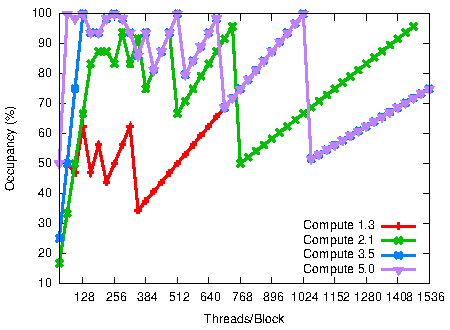
\includegraphics[width=0.8\textwidth]{images/impl/occupancy/occupancy}
    \caption[Impact of varying thread block size on multiprocessor occupancy]{
        Illustration of the impact of varying the thread block size on the
        overall multiprocessor occupancy. The example kernel requires 22
        registers per thread and 16 bytes of shared memory per thread. Each
        device generation (compute capability) achieves peak occupancy at
        different points in the sequence, so selecting a static thread block
        size for all kernels and devices is clearly suboptimal. Older devices
        are unable to achieve 100\% occupancy due to limitations in the register
        file size and available shared memory. The first two generations of
        devices can not execute the kernel with more than 704 and 1472 threads
        per block respectively.}
    \label{fig:occupancy}
\end{figure}


\subsection{Kernel execution}

To evaluate the array computation on the CUDA backend, we perform a bottom-up
traversal of the annotated program (\S\ref{sec:annotating_array_programs})
executing the attached kernels. For each node of the AST, we distinguish three
cases:
%
\begin{enumerate}
\item If it is a @Use@ node, return a reference to the device memory holding the
    array data.

\item If it is a non-skeleton node, such as a let binding or shape conversion,
    the evaluator executes the operation directly by adjusting the environment
    or similar as required.

\item If it is a skeleton node, memory is allocated to hold the result of
    evaluating the skeleton, and finally invokes the one or more GPU kernels
    that implement the operation.
\end{enumerate}
%
In summary, the execution pass interleaves host-side evaluation and the
invocation of GPU kernels, while keeping track of device memory, allocating
intermediates, and releasing memory once no longer required. See
Section~\ref{sec:memory_management} for details on memory management. GPU
kernels execute asynchronously, so the evaluator is able to immediately begin to
set up the next stage of the computation while the current kernel executes. The
CUDA runtime maintains the sequence of kernels to be executed on the device,
known as the execution \emph{stream}.
% so if the result of an asynchronously executing kernel is needed before the
% kernel completes, any kernels that depend on that result will only be invoked
% after the kernel completes.

\subsection{Kernel execution, concurrently}

Beginning with compute capability 2.0, some CUDA devices are able to execute
multiple kernels concurrently, rather than always executing kernels one after
the other. This can improve overall performance by increasing the number of
active threads on the device, particularly when executing many small kernels.
Accelerate's collective operations have a purely functional semantics, so
concurrent expression evaluation is always sound. The current implementation
executes subtrees of the expression concurrently on the single device. We leave
for future work additionally executing programs concurrently on separate GPUs,
as is available in some Tesla configurations.

In order to execute kernels concurrently, the kernels must be issued in
different non-default streams. A \emph{stream}\cuda[stream]{} is a sequence of
commands that execute in order; different streams, on the other hand, may
execute their commands out of order with respect to one another or concurrently.
To allow streams to synchronise, an \emph{event}\cuda[event]{} may be inserted
into a stream. Any stream may delay execution until a given event has been
posted, which allows efficient cross-stream synchronisation that is managed by
the device.

The Accelerate CUDA backend introduces concurrency when evaluating the bound
expression at a let binding, and synchronises when looking up a bound variable
in the environment. Following conversion and optimisation of the program by the
Accelerate frontend, any operation that is to be evaluated will appear as a
let-bound expression in the program, and so sequences of let bindings may be
able to execute their subtrees concurrently. The array expression evaluator has
the type:
%
\begin{lstlisting}[style=haskell]
executeOpenAcc
    :: ExecOpenAcc aenv arrs            -- annotated array program (\S\ref{sec:annotating_array_programs})
    -> Aval aenv                        -- array environment with synchronisation points
    -> Stream                           -- current execution stream
    -> CIO arrs
\end{lstlisting}
%
The array environment is augmented to carry both the array object as well as an
event execution streams can synchronise against, which signals that the array
has been fully evaluated:
%
\begin{lstlisting}[style=haskell]
data Async a = Async Event a

data Aval env where
  Aempty :: Aval ()
  Apush  :: Aval env -> Async t -> Aval (env, t)
\end{lstlisting}

The only interesting cases for the evaluator are those of let bindings and
environment lookup. When looking up an array in the environment, we ensure that
all future work submitted to the current stream will occur after the
asynchronous event for the array in the environment has been fulfilled.
Synchronisation occurs on the device, so the following does not block waiting
for the result:
% \footnote{\footcode{Event.wait} is the FFI binding to \footcode{cudaStreamWaitEvent} and comes from the CUDA binding library.}
%
\begin{lstlisting}[style=haskell]
after :: Stream -> Async a -> CIO a
after stream (Async event arr) = Event.wait event (Just stream) [] >> return arr
\end{lstlisting}

Evaluating the binding of a let requires evaluating the expression in a new
asynchronous execution stream. The body expression is then evaluated with the
bound array wrapped in an @Async@, which contains the event indicating when the
last kernel issued to the stream has completed.
%
\begin{lstlisting}[style=haskell]
streaming :: Context
          -> Reservoir
          -> (Stream -> CIO a)
          -> (Async a -> CIO b)
          -> CIO b
streaming ctx rsv`(Reservoir _ weak_rsv) bnd body = do
    stream <- create ctx rsv                                                       -- (1)
    bnd'   <- bnd stream                                                           -- (2)
    end    <- Event.waypoint stream
    body'  <- body (Async end bnd')                                                -- (3)
    destroy (weakContext ctx) weak_rsv stream                                      -- (4)
    Event.destroy end
    return body'
\end{lstlisting}
%
\begin{enumerate}
\item The function @create@ allocates a new execution stream. It uses a
    technique similar to the @Nursery@
    (\S\ref{sec:memory_manager_implementation}) to reuse execution streams that
    are currently idle, taking an inactive stream from the @Reservoir@ if one is
    available, or allocating a new execution stream otherwise.
%
% \begin{lstlisting}[style=haskell]
% type RSV        = MVar ( HashTable CUDA.Context (FullList () Stream) )
% data Reservoir  = Reservoir RSV (Weak RSV)
% \end{lstlisting}

\item The bound expression is executed asynchronously, assigned to the new
    @Stream@.

\item The body of the expression is evaluated. The extended array environment
    includes the event @end@, which will be signalled once the result of the
    binding is available.

\item In contrast to the memory manager, events and streams never remain active
    beyond the evaluation of the Accelerate program, so the stream and event
    event associated with evaluating the binding are explicitly deallocated
    after evaluation of the body completes.

\end{enumerate}

As an example, Listing~\ref{lst:concurrent_kernels} contains an example program
that is able to execute the nine @map@ operations concurrently on devices of
compute capability 2.0 and greater. Note that, to keep the example simple,
fusion is disabled to prevent the @map@ operations from fusing into the @zip9@.
The corresponding execution trace from the NVIDIA Visual Profiler application is
shown in Figure~\ref{fig:concurrent_kernels}, which demonstrates each of the
@map@ operations executing in separate streams and overlapping with each other.

\begin{lstlisting}[style=haskell_float
    ,float
    ,label=lst:concurrent_kernels
    ,caption={[Example program that executes kernels concurrently]
        An example program that executes each of the \code{map} kernels
        concurrently, on devices of compute capability 2.0 and greater. Note
        that in order to keep the example simple, the displayed behaviour is
        only seen when fusion is disabled, to prevent the operations from being
        combined into a singel kernel.}]
loop :: Exp Int -> Exp Int
loop ticks = A.while (\i -> i <* clockRate * ticks) (+1) 0
  where
    clockRate   = 900000

concurrentTest :: Acc (Vector (Int,Int,Int,Int,Int,Int,Int,Int,Int))
concurrentTest
  = A.zip9 (A.map loop (use $ fromList Z [1]))
           (A.map loop (use $ fromList Z [1]))
           ...
\end{lstlisting}

\begin{figure}[tbp]
    \centering
    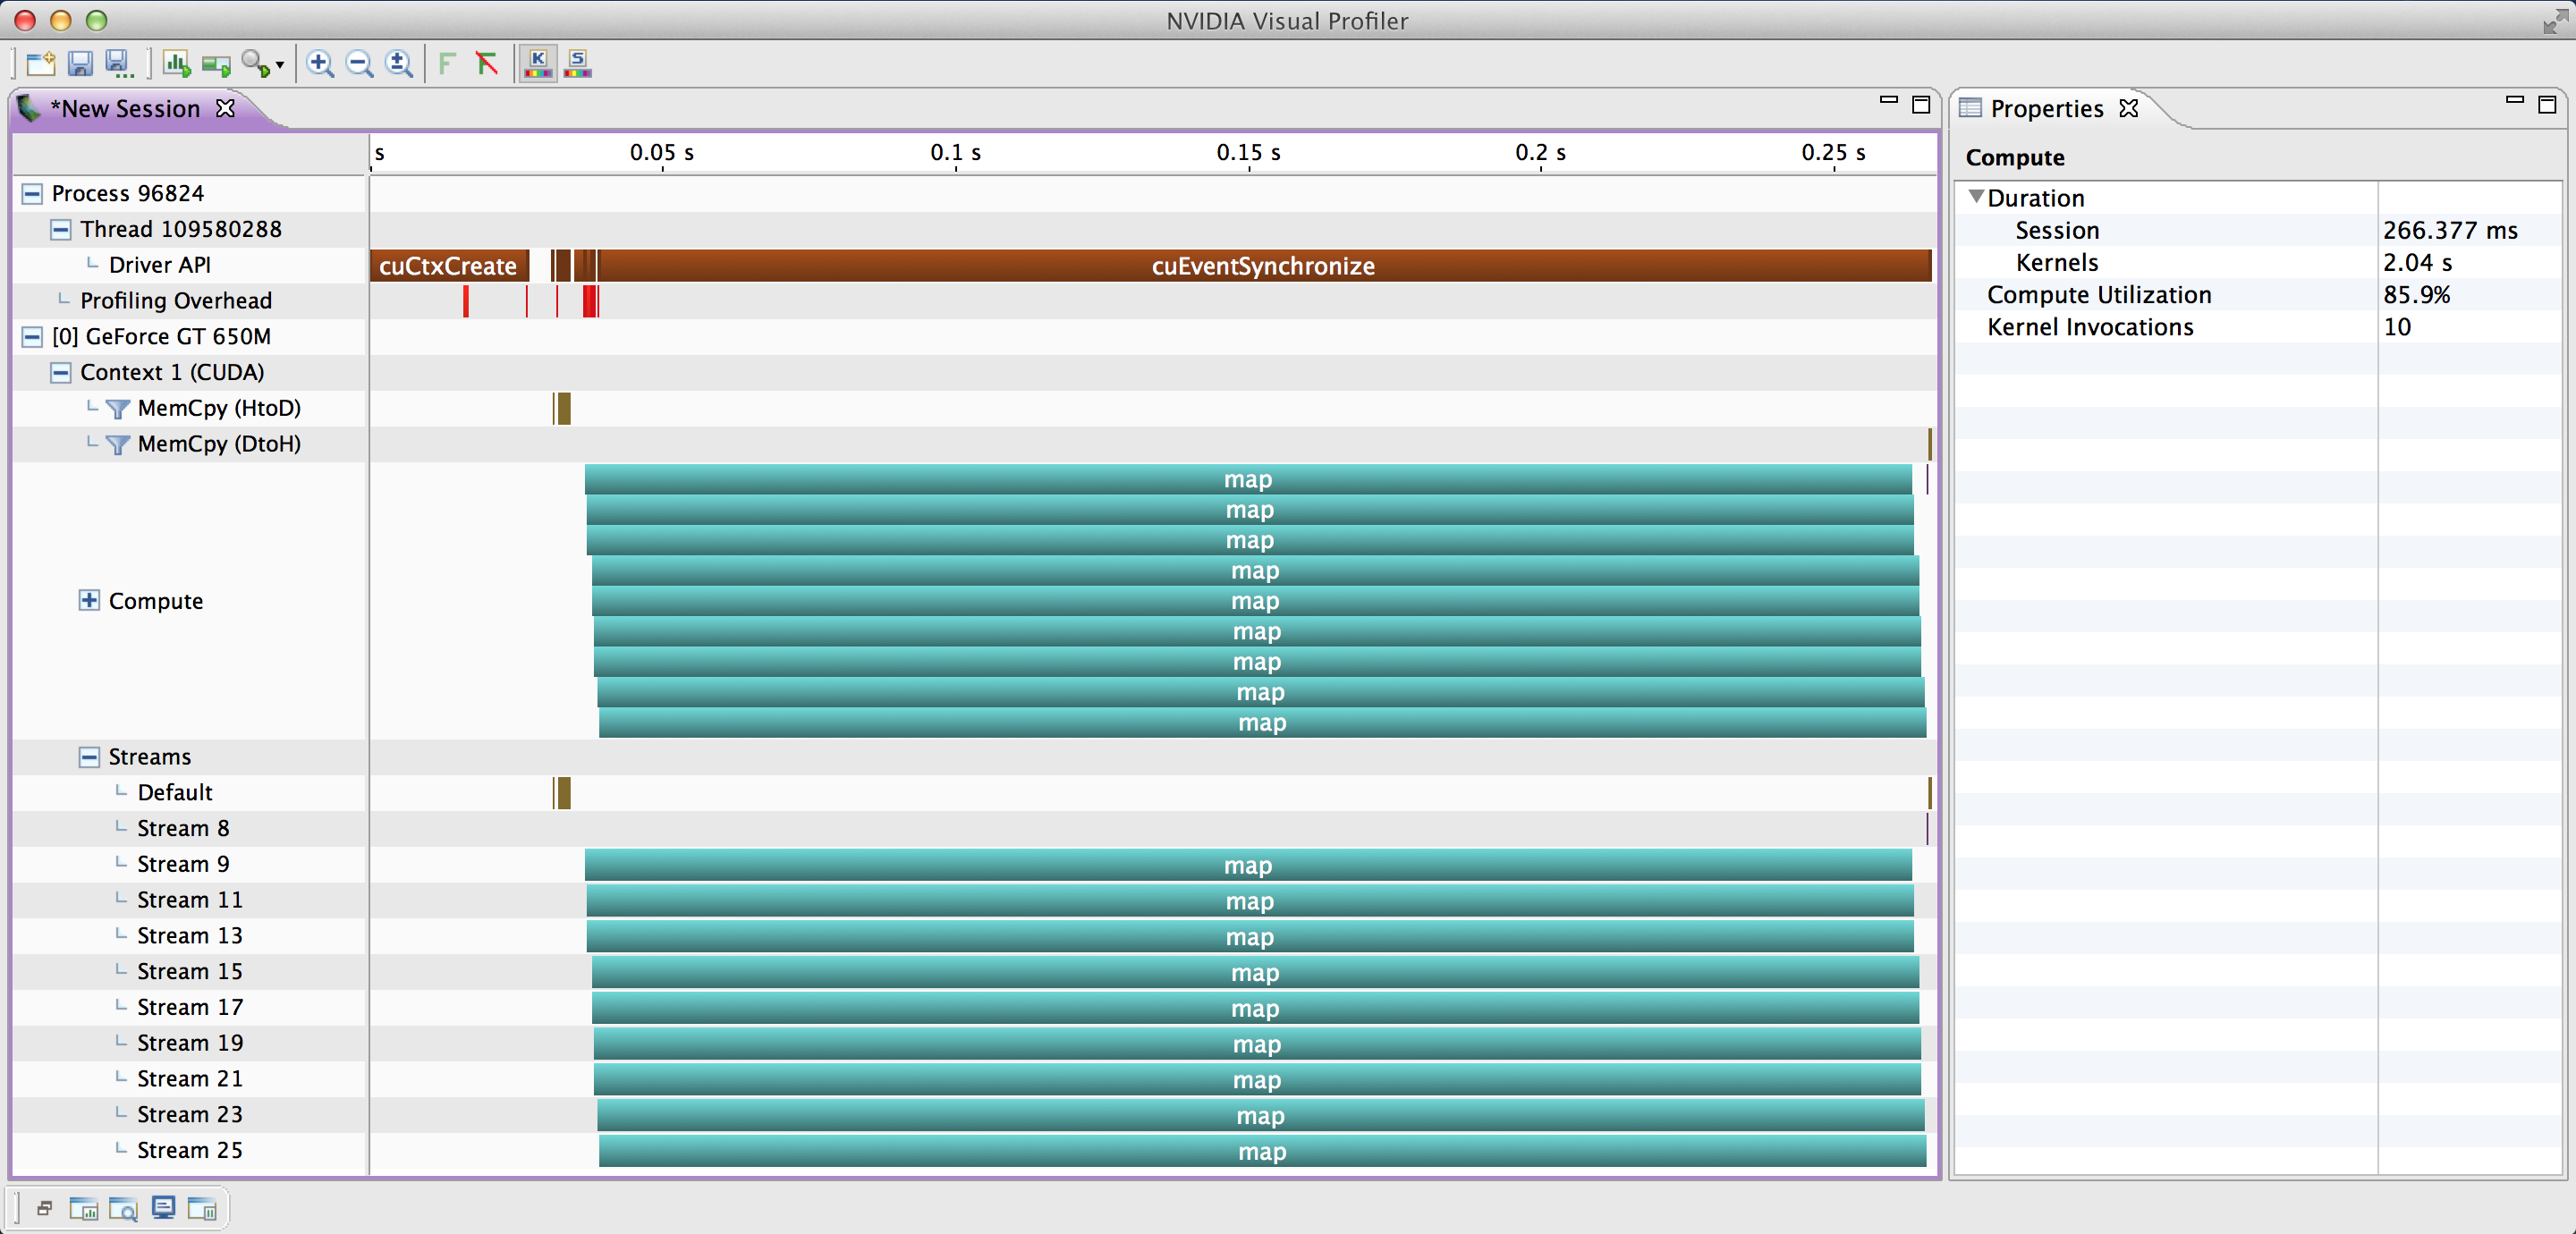
\includegraphics[width=\textwidth]{images/impl/concurrent_kernels}
    \caption[Profiling trace of a program which executes kernels
    concurrently]{Trace from the NVIDIA Visual Profiler application for the
    program shown in Listing~\ref{lst:concurrent_kernels}, where the nine
    \code{map} kernels execute concurrently on devices of compute capability 2.0
    and greater. Each \code{map} operation takes $226.7$~ms to execute. As
    shown, an equivalent of $2.04$~seconds of GPU time is execute in a wall
    clock time of $266.4$~ms, which includes program initialisation.}
    \label{fig:concurrent_kernels}
\end{figure}

\subsubsection{Interaction with Array Fusion}

In the example shown in Listing~\ref{lst:concurrent_kernels}, it was necessary
to disable the array fusion optimisation (\S\ref{sec:array_fusion}) in order to
prevent the kernels being combined into a single kernel, within which each of
the fused operations execute sequentially. While a simple example was chosen on
purpose in order to clearly demonstrate kernels executing concurrently, the same
situation nevertheless arises in real programs. That is, by combining sequences
of operations into a single operation, fusion has the effect of removing
opportunities for concurrent kernel execution.

It is left to future work to provide some analysis of when it would be
beneficial to avoid fusing operations, on the basis that it would be more
efficient to instead execute the two sub-computations concurrently. Such an
analysis would need to take into account the hardware that the program is to be
executed on, as well as an estimate of how much of the GPU's resources each
kernel requires. This is required in order to determine if the two kernels could
be scheduled concurrently.


\subsection{Conclusion}

Runtime system operations are important, as they partially compensate for the
overhead of being an embedded language; that is, of needing to traverse the
program AST in order to evaluate it. The Accelerate runtime system is designed
to execute programs as efficiently as possible, which in turn helps maximise the
computational utilisation of the device, and ensure all processors are kept
busy.

The runtime system attempts to optimise both individual kernel executions, as
well as execution of the entire program. In the former case, each kernel launch
is configured to maximise thread occupancy for the particular device the kernel
is being executed on, and kernels are scheduled such that independent operations
can be executed concurrently, on devices which support this. The single most
important optimisation, however, is that each node of the program AST is
decorated with all of the data required to execute that operation. For programs
which are executed more than once, this means that the costly front-end analysis
and code generation steps of program execution can be skipped on the second and
subsequent invocations of the program, and kernels can begin executing
immediately. This process happens automatically, and almost\footnote{The user
must express their program in the form of a function of one array argument,
and use the corresponding \code{run1} function to execute the program. This is
not so onerous, as any operation that the user intends to execute multiple times
is likely to be easily written in the form of a function from arrays to arrays.}
entirely transparently to the user.

With these optimisations, the Accelerate runtime system is efficient enough that
we can execute numerically intensive programs such as fluid flow simulations
(\S\ref{sec:fluid}) and real-time image processing applications
(\S\ref{sec:canny}) and achieve performance comparable to hand-written CUDA
programs.


\section{Related work}
\label{sec:implementation_related}

The development of general-purpose applications that run on the GPU is highly
work intensive, and has been estimated to require at least $10\times$ as much
effort as developing an efficient single-threaded
application~\cite{Sweeney:2009ua}. Several researchers have proposed to
ameliorate the status quo by either using a high-level library to compose GPU
code or by compiling a subset of a high-level language to low-level GPU code.
This section explores some of these approaches.


\subsection{Embedded languages}

%% Haskell-based approaches

% Vertigo~\cite{Elliott:2004hh} is an embedded language in Haskell for 3D
% graphics. Vertigo is a statically compiled graphics language targeting the
% DirectX shader model, and does not offer higher-order combinators such as @map@
% and @fold@, but does feature an optimising compiler.

Obsidian~\cite{Svensson:2008a,Svensson:2013wd} and Nikola~\cite{Mainland:2010vj} are also
Haskell EDSLs for GPGPU programming, and are in aim and spirit the embeddings
closest to Accelerate. Both Nikola and Obsidian produce CUDA code as we do,
however while we use algorithmic skeletons (\S\ref{sec:code_generation}), Nikola
explicitly schedules loops, limiting it to @map@-like operations, and Obsidian
is a lower level language where more details of the GPU hardware are exposed to
the programmer. Both Nikola and Obsidian lack any system of kernel caching,
memory management, or any significant runtime system or compilation
optimisations. In both Obsidian and Nikola, algorithms spanning multiple kernels
need to be explicitly scheduled by the application programmer and incur
additional host-device data transfer overhead, which incurs as severe
performance penalty.

% \marginnote{tk: to related work for fusion?}
% Recent versions of Obsidian~\cite{Claessen:2012hl} implement
% Repa-style~\cite{Keller:2010er} delayed \emph{pull arrays} as well as \emph{push
% arrays}. Whereas a pull array represents a general producer, a push array
% represents a general consumer. Pull arrays allow intermediate programs to be
% written in continuation passing style (CPS)\index{continuation passing style},
% which helps to compile (and fuse) append-like operations.

Paraiso~\cite{Muranushi:2012eh} is a Haskell EDSL for solving systems of
partial differential equations (PDEs), such as hydrodynamics equations,
and generates both CUDA code for GPUs as well as OpenMP~\cite{OpenMP:2008} code
for multicore CPUs. Accelerate supports @stencil@ operations for expressing this
class of operation, but lacks the domain specific language features and compiler
optimisations implemented by Paraiso for this type of problem. Paraiso also
features an automated tuning framework that will search for faster
implementations of the program, guided by user annotations.

Baracuda~\cite{Larsen:2011fa} is a Haskell EDSL producing CUDA GPU kernels,
though it is intended to be used offline, with the kernels called directly from
a C++ application. It supports only @map@ and @fold@ over vectors.


\subsection{Parallel libraries}

%% C++-based approaches

Accelerator~\cite{Bond:2010bd,Tarditi:2006} is a C++ library-based approach with
less syntactic sugar for the programmer, but does have support for bindings to
functional languages. In contrast to our current work, it already targets
multiple architectures, namely GPUs, FPGAs, and multicore CPUs. However, the
code generated for GPUs uses the DirectX 9 API, which does not provide access to
several modern GPU features, negatively impacting performance and preventing
some operations such as scatted writes.

RapidMind~\cite{LinXu:2008ig}, which targets the GPU using OpenCL, and its
predecessor Sh~\cite{McCool:2004,McCool:2004un} which used pixel shaders of the
graphics API, are C++ meta programming libraries for data parallel programming.
RapidMind was merged into Intel's Ct compiler to create the Array Building
Blocks (ArBB) library. However, the ArBB project was retired before support for
GPUs was integrated. GPU++~\cite{Jansen:2008vw} is an embedded language in C++
using similar techniques to RapidMind and Sh, but provides a more abstract
interface than the other C++ based methods listed here.

Thrust~\cite{ThrustAParallelT:ub} is a library of algorithms written in CUDA,
with an interface similar to the C++ Standard Template Library.
\citet{Sato:2009cq} describe a C++ library for GPGPU programming based on
algorithmic skeletons. Both of these libraries can be used to generate both CUDA
code for the GPU as well as OpenMP code targeting multicore CPUs.


%% other approaches

Dandelion~\cite{Rossbach:2013bj} is a library of data-parallel operations,
specified as comprehensions on arrays using the LINQ framework for .NET
(programmers write in either C@#@ or F@#@). Operations are compiled for the GPU
as well as the CPU, and the runtime system distributes the computation over all
of the available processors in a heterogeneous cluster.

PyCUDA~\cite{Klockner:2012tj} provide low-level access to the CUDA driver API
from within Python, and facilitates runtime code generation for the GPU\@. A
similar approach is taken by CLyther~\cite{CLyther:EvXSiruK} which targets
OpenCL. Copperhead~\cite{Catanzaro:2011cn} uses PyCUDA and Thrust internally to
provide a higher level of abstraction to compile, link, cache, and execute CUDA
code. Both Parakeet~\cite{Rubinsteyn:2012ve} and Anaconda
Accelerate~\cite{AnacondaAccelerate:2013vn} are Python libraries that attempt to
just-in-time compile a subset of Python code that uses the
NumPy~\cite{NumPy:2006uq} array library to instead target the GPU\@.

Jacket~\cite{AccelerEyes:vq} is a Matlab extension that allows matrix
computations to be offloaded to the GPU, by introducing new datatypes and
operations for transferring matrices to GPU memory, and overloading operations
on those matrices to trigger execution of suitable GPU kernels.


\subsection{Other approaches}

Delite/LMS~\cite{Rompf:2013er} is a compiler framework for writing parallel domain
specific languages in Scala. It includes several backend code generation targets
including C++ and CUDA\@.

Nesl/GPU~\cite{Bergstrom:2012bi} compiles NESL~\cite{Blelloch:1995ut} code to
CUDA, a system which was independently developed as CuNesl~\cite{Zhang:2012jl}.
Performance suffers because the implementation relies on the legacy NESL
compiler, which produces a significant number of intermediate computations.

NOVA~\cite{Collins:2013wn} is a high-level lisp-like functional language and
compiler for parallel operations, targeting both GPUs and CPUs. Compared to
Accelerate, NOVA supports fewer parallel operations, but does claim to support
nested parallelism, recursion, and sum data types. The NOVA compiler has not
been released, so these claims can not be tested.


\section{Discussion}

This chapter has detailed the implementation of the CUDA generating Accelerate
backend targeting parallel execution on NVIDIA GPUs. We discussed our approach
to skeleton-based code generation, as well as the caching mechanisms that are
implemented in order to reduce the overheads of the embedding, such as of
runtime code generation and compilation. This chapter also dealt with the issue
of memory management and data transfer, which is a key consideration to
achieving high performance. Finally, we discussed the execution of the generated
GPU kernels, including launch configuration and concurrent execution
optimisations, in order to maximise device utilisation and help reduce overall
program run times.

Now that we can compile and run Accelerate programs on the GPU, the next chapter
covers how to optimise Accelerate programs. In particular, we introduce our
type-safe approaches to sharing recovery and array fusion, which we identify as
the two most pressing performance limitations.


% \marginnote{perhaps split differently: real vs. embedded languages?}
% 
% Other significant parallel or GPGPU programming models and languages.
% Limitations that we share/avoid. Where we differ
% \begin{itemize}
% \item Repa \cite{Keller:2010er,Lippmeier:2011cd,Lippmeier:2012gx} (Haskell)
% \item SkeTo \cite{Matsuzaki:2011ew} (C++)
% \item list homomorphism based \cite{Sato:2009cq} (C++)
% \item Delite/LMS \cite{Rompf:2013er} (Scala)
% \item Nesl/GPU \cite{Bergstrom:2012bi} (Haskell)
% \item Nikola \cite{Mainland:2010vj} (Haskell)
% \item Obsidian \cite{Svensson:2008a,Claessen:2012hl} (Haskell)
% \item Baracuda \cite{Larsen:2011fa} (Haskell)
% \item Jacket/ArrayFire \cite{AccelerEyes:vq} (Matlab)
% \item Anaconda Accelerate \cite{AnacondaAccelerate:2013vn} (Python)
% \item NOVA \cite{Collins:2013wn} (lisp)
% \item Dandelion \cite{tk} (LINQ)
% \end{itemize}



%
% END
%

%\begin{itemize}
%\item implementing parallel algorithms (20\%, 1 week)
%    \begin{itemize}
%        \item fold
%        \item scan
%        \item permute (atomic operations)
%        \item segmented/rank polymorphic operations
%    \end{itemize}
%
%\item skeleton-based code generation (2 weeks)
%    \begin{itemize}
%        \item device capabilities (free array variables, @umul24@,
%            @shfl@, atomic operations, shared memory)
%        \item rank polymorphic operations
%    \end{itemize}
%
%\item runtime system (3 weeks)
%    \begin{itemize}
%        \item launching kernels (occupancy calculator)
%        \item caching compiled kernels (live \& persistent caches)
%        \item memory management (escaping the EDSL evaluator; weak pointers vs.
%            reference counting)
%        \item executing kernels (annotated AST)
%    \end{itemize}
%
%\end{itemize}

% \begin{itemize}
%\item Accelerate frontend
%    \begin{itemize}
%        \item reification
%            \begin{itemize}
%                \item smart constructors for type classes
%                \item explicit dictionaries (polymorphism)
%                \item environments
%                \item HOAS vs. de Bruijn
%                \item representation types
%            \end{itemize}
%        \item surface \& internal (core) languages
%            \begin{itemize}
%                \item representing different constructs in surface/core
%                \item surface nested $\rightarrow$ core flat ?? (fuuuuture)
%            \end{itemize}
%        \item sharing observation ( --> sec 5? not my work )
%    \end{itemize}
%
%\item Accelerate CUDA backend
%    \begin{itemize}
%        \item code generation
%            \begin{itemize}
%                \item architecture sensitive JIT cross-compiler
%                \item future work: types, Haskell compile time
%            \end{itemize}
%        \item external compilation
%            \begin{itemize}
%                \item annotating AST nodes
%            \end{itemize}
%        \item memory management
%            \begin{itemize}
%                \item weak pointers \& weak hash tables
%                \item advantages to alternatives
%            \end{itemize}
%        \item execution
%            \begin{itemize}
%                \item occupancy analysis
%                \item multi-pass kernels
%            \end{itemize}
%        \item performance
%            \begin{itemize}
%                \item amortizing overheads (how to quantise this?)
%                \item of generated code
%                \item runtime overheads
%                \item w.r.t. CUDA memory subsystem (theoretical performance)
%                \item examples! spot the infelicities! (dot product)
%            \end{itemize}
%    \end{itemize}
%\end{itemize}

%Compilation has five phases:
%\begin{itemize}
%    \item Lexing
%    \item Parsing
%    \item Semantic analysis
%    \item Optimisation
%    \item Code Generation
%\end{itemize}

% EDSL basics:
%
% http://www.haskell.org/haskellwiki/Embedded_domain_specific_language
% http://www.haskell.org/haskellwiki/Research_papers/Domain_specific_languages
% 
% There are two major degrees of embedded languages:
% 
% \begin{description}
% \item[Shallow:] Operations immediately translate into the target language.
% 
% \item[Deep:] Operations build a data-structure that reflects the expression to
%     be evaluated. This structure allows the expression to be transformed before
%     being translated into the target language; for example by applying
%     optimisations.
% \end{description}
% 
% Sharing and recursion are common problems when implementing embedded domain
% specific languages.


\chapter{Optimising embedded array programs}
\label{ch:optimising}

\epigraph{Relax. As usual, I will bore you with the details.}%
{\textsc{---chris lee}}

The previous chapter discussed the architecture of the Accelerate language
embedding and execution on CUDA hardware. Through a set of benchmarks, our
previous work~\cite{Chakravarty:2011fr} identified the two most pressing
performance limitations: operator fusion and data sharing. This chapter
describes the methods used to overcome these issues, focusing primarily on my
novel approach to operator fusion in the context of the stratified Accelerate
language and skeleton-based implementation of the CUDA backend. This chapter
expands upon the ideas that appeared in~\cite{McDonell:2013wi}.

It should be noted that ``optimisation'' is a misnomer; only rarely does
applying optimisations to a program result in object code whose performance is
optimal, by any measure. Rather, the goal is to \emph{improve} the performance
of the object code generated by a backend, although it is entirely possible that
they may decrease it or make no difference at all. As with many interesting
problems in [computer] science, in most cases it is formally undecidable whether
a particular optimisation improves, or at least does not worsen, performance.

In general, we would like to be as aggressive as possible in improving code, but
not at the expense of making it incorrect.


% \section{Redundancy Elimination}
% \label{sec:redundancy_elimination}
%
% The optimisations in this section deal with the elimination of redundant
% computations. These procedures almost always improve the performance of the code
% they are applied to.

\section{Sharing recovery}
\label{sec:sharing_recovery}

\begin{lstlisting}[style=haskell_float
    ,float=t
    ,label=lst:blackscholes
    ,caption={Black-Scholes option pricing}]
riskfree, volatility :: Float
riskfree   = 0.02
volatility = 0.30

horner :: Num a => [a] -> a -> a
horner coeff x = x * foldr1 madd coeff
  where
    madd a b = a + x*b

cnd' :: Floating a => a -> a
cnd' d =
  let poly     = horner coeff
      coeff    = [0.31938153, -0.356563782, 1.781477937, -1.821255978, 1.330274429]
      rsqrt2pi = 0.39894228040143267793994605993438
      k        = 1.0 / (1.0 + 0.2316419 * abs d)
  in
  rsqrt2pi * exp (-0.5*d*d) * poly k

blackscholes :: Vector (Float, Float, Float) -> Acc (Vector (Float, Float))
blackscholes = map callput . use
  where
  callput x =
    let (price, strike, years) = unlift x
        r       = constant riskfree
        v       = constant volatility
        v_sqrtT = v * sqrt years
        d1      = (log (price / strike) + (r + 0.5 * v * v) * years) / v_sqrtT
        d2      = d1 - v_sqrtT
        cnd d   = let c = cnd' d in d >* 0 ? (1.0 - c, c)
        cndD1   = cnd d1
        cndD2   = cnd d2
        x_expRT = strike * exp (-r * years)
    in
    lift ( price * cndD1 - x_expRT * cndD2                      -- call price
         , x_expRT * (1.0 - cndD2) - price * (1.0 - cndD1))     -- put price
\end{lstlisting}

Accelerate is a \emph{deeply embedded} language, meaning that evaluating an
Accelerate program does not directly issue computations; instead, it builds an
\emph{abstract syntax tree} (AST\AST{}) that represent the embedded computation
(\S\ref{sec:EDSLs}). This AST is later executed by an Accelerate backend to
compute the result on a given backend target (\S\ref{sec:executing_programs}).

A well known problem of defining deeply embedded languages in this way is the
issue of \indexe{sharing}. The deeply embedded language implementation of
Accelerate reifies the abstract syntax of the deeply embedded language in
Haskell. However, a straightforward reification of the surface language program
results in each occurrence of a let-bound variable in the source program
creating a separate unfolding of the bound expression in the compiled code.

As an example, consider the pricing of European-style options using the
Black-Scholes formula, the Accelerate program for which is shown in
Listing~\ref{lst:blackscholes}. Given a vector with triples of underlying stock
price, strike price, and time to maturity (in years), the Black-Scholes formula
computes the price of a call and put option. The function @callput@ evaluates
the Black-Scholes formula for a single triple, and @blackscholes@ maps it over a
vector of triples, such that all individual applications of the formula are
executed in parallel.

The function @callput@ introduces a significant amount of sharing: the helper
functions @cnd'@ and hence also @horner@ are used twice --- for @d1@ and @d2@
--- and its argument @d@ is used multiple times in the body. Worse, the
conditional expression leads to a growing number of predicated instructions
which incurs a large penalty on the SIMD architecture of a GPU\@. A lack of
sharing recovery was a significant shortcoming of our initial implementation of
Accelerate~\cite{Chakravarty:2011fr}.

% As described in Section~TK, operations of the embedded language do not
% directly issue computations; instead, they build \emph{abstract syntax
% trees}\index{abstract syntax tree}\index{AST|see{abstract syntax tree}} that
% represent the embedded computation. These term trees use \indexe{higher-order
% abstract syntax} (HOAS)\index{higher-order abstract syntax} to embed
% function-valued scalar expressions as well as typeclass overloading to reflect
% arithmetic expressions.
%
% However, a straightforward reification of the surface language program results in a
% complete unfolding of the expression into embedded language terms. That is, each
% occurrence of a let-bound variable in the source program would create a separate
% unfolding of the bound expression in the compiled code. For example, consider
% the following program:
% %
% \begin{lstlisting}[style=Haskell]
% let ys = map f xs
% in  zipWith g ys ys
% \end{lstlisting}
% %
% If we do not take care, the expression will be inefficiently translated as:
% %
% \begin{lstlisting}[style=Haskell]
% zipWith g (map f xs) (map f xs)
% \end{lstlisting}


\subsection{Our approach to sharing recovery}
\index{sharing!recovery|(}

This problem was solved elegantly by \citet{Gill:2009dx} who proposed the use
of \index{stable name}\emph{stable names}~\cite{PeytonJones:2000ks} to recover
sharing of source terms in a deeply embedded language. Unfortunately, Gill's
original approach (1) reifies the abstract syntax in \emph{graph} form, and (2)
assumes an \emph{untyped} syntax representation. We use a variant of Gill's
technique that instead preserves types and produces a tree with minimal
flattening, which is able to recover exactly those let bindings which appear in
the source program~\cite{McDonell:2013wi}.

The higher-order abstract syntax (HOAS\HOAS{}) representation of the surface
language, while convenient for the human reader, is awkward for program
transformations as it complicates looking under lambdas. We convert the source
representation to a type-safe internal representation based on nameless de
Bruijn indices in the style of \citet{Altenkirch:2003kz}, using GADTs
\cite{Jones:2006eh} and type families
\cite{Chakravarty:2005dx,Schrijvers:2008ir} to preserve the embedded program's
type information. While developed independently
\cite{McDonell:2013wi,Chakravarty:2009uo}, this conversion is similar to the
\emph{unembedding} of \citet{Atkey:2009dj}. Unembedding and sharing recovery are
necessarily intertwined. Sharing recovery must be performed on the source
representation, otherwise sharing will have already been lost, but we can not
perform sharing recovery on higher-order abstract syntax as we need to traverse
below the lambda abstractions. Hence, both operations go hand in hand.

\begin{figure}
\centering
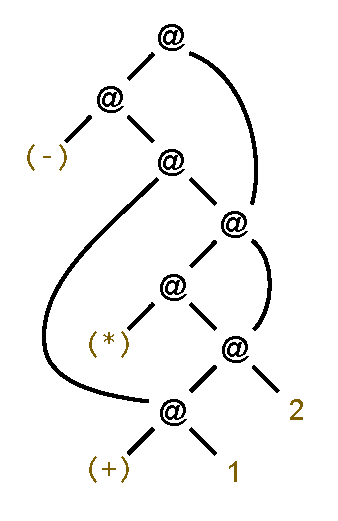
\includegraphics[scale=0.5]{images/opt/sharing-original}
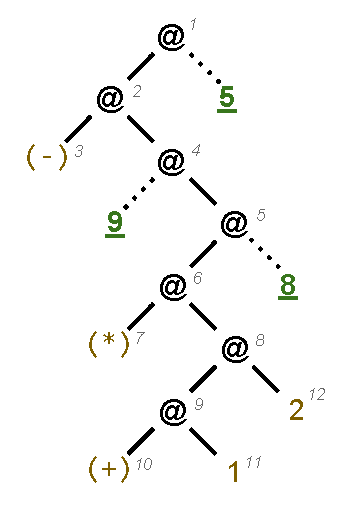
\includegraphics[scale=0.5]{images/opt/sharing-pruned}
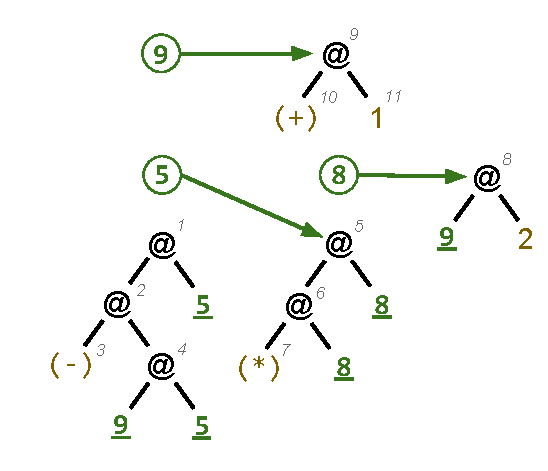
\includegraphics[scale=0.5]{images/opt/sharing-floated}
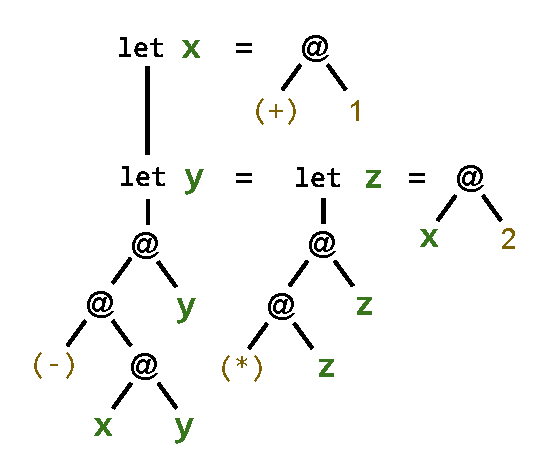
\includegraphics[scale=0.5]{images/opt/sharing-lets}
\caption{Recovering sharing in an example term}
\label{fig:sharing_recovery}
\end{figure}

The contribution of the sharing recovery algorithm is work done primarily by my
supervisor Manuel Chakravarty, so I present here only a brief overview of the
method; see \cite{McDonell:2013wi} for details. Consider the following source
term:
%
\begin{lstlisting}[style=haskell]
let inc = (+1) 1
in let nine = let three = inc 2
              in
              (*) three three
in
(-) (inc nine) nine
\end{lstlisting}
%
The term's abstract syntax DAG is shown as the left-most diagram in
Figure~\ref{fig:sharing_recovery}, which uses \app\ nodes to represent
application. Typed conversion from HOAS with sharing recovery proceeds in three
stages:


\subsubsection*{Phase 1: Prune shared terms:}

Phase one is a depth-first traversal of the AST which annotates each node with
its unique \indext{stable name}, and builds an occurrence map for the number of
times each node is seen in the overall program. The stable names of two Haskell
terms are equal only when the terms are represented by the same heap structure
in memory. Likewise, when the AST of two terms of an embedded language program
have the same stable name, we know that they represent the same term. If we
encounter a node already in the occurrence map, it represents a previously
visited node and is thus a \emph{shared subterm}. We replace the entire subterm
at that node with a placeholder containing its stable name. The second diagram
in Figure~\ref{fig:sharing_recovery} shows the outcome of this stage. Each node
is labelled by a number that represents its stable name, and the dotted edges
indicate where we encountered a previously visited, shared node. The
placeholders are indicated by underlined stable names. In this way all but the
first occurrence of a shared subterm are pruned,
%and replaced with variable bindings,
and we do not descend into terms that have been previously encountered. This
avoids completely unfolding the embedded expression, so the complexity of
sharing observation is proportional to the number of nodes in the tree
\emph{with} sharing.%
\footnote{Since computing stable names requires the use of Haskell's
\footcode{IO} monad, we can use a hash table to store the occurrence counts and
thereby keep the complexity of Phase 1 as
$\mathcal{O}\left(n\right)$.}%
\footnote{This is also why we do not use redundancy elimination techniques such
as global value numbering or common subexpression elimination, as those methods
are applied to the completely unfolded expression.}

As the stable name of an expression is an intensional property, it can only be
determined in Haskell's @IO@ monad, and strictly speaking, because of this
it is not deterministic. The stable name API does not guarantee completeness:
for two stable names @sn1@ and @sn2@, if @sn1 == sn2@ then the
two stable names were created from the same heap object. However, the reverse is
not necessarily true; if the two stable names are not equal the objects they
come from may still be equal. Put another way, equality on stable names may
return a false negative, which means that we fail to discover some sharing, but
can never return a false positive since stable names from different heap objects
are not considered equal. Luckily, sharing does not affect the denotational
meaning of the program, and hence a lack of sharing does not compromise
denotational correctness.


\subsubsection*{Phase 2: Float shared terms:}

The second phase is a bottom-up traversal of the AST that determines the scope
for every shared binding that will be introduced. It uses the occurrence map to
determine, for every shared subterm, the meet of all the shared subterm
occurrences --- the lowest AST node at which the binding for the subterm can be
placed. This is why the occurrence map generated in the previous phase can not
be simplified to a set of occurring names: we need the actual occurrence count
to determine where shared subterms should be let-bound.

The third diagram of Figure~\ref{fig:sharing_recovery} shows the result of this
process. Floated subterms are referenced by circled stable names located
\emph{above} the node that they floated to. If the node collects more than one
shared subterm, the subterm whose origin is deeper in the original term goes on
top; here, 9 on top of 5. Nested sharing leads to subterms floating up inside
other floated subterms; here, 8 stays inside the subterm rooted at 5.


\subsubsection*{Phase 3: Binder introduction:}

Finally, each floated subterm gets let-bound right above the node it floated to,
as shown in the rightmost diagram of Figure~\ref{fig:sharing_recovery}. At the
same time, the AST is converted into nameless de Bruijn form by introducing de
Bruijn indices at the same time as introducing the lets.

\index{sharing!recovery|)}

\section{Array fusion}
\label{sec:array_fusion}

Fusion, or deforestation, is a term used to describe techniques for having a
compiler automatically eliminate intermediate data structures in a computation
by combining successive traversals over these data structures. For example, to
compute the sum of squares of all integers from one to a given number in
Haskell~\cite{Haskell:1998}, one could write:
%
\begin{lstlisting}[style=haskell]
sum_of_squares :: Int -> Int
sum_of_squares n
    = sum                       -- add all numbers in the list
    $ map (\x -> x * x)         -- traverse list doubling each element
    $ enumFromTo 1 n            -- generate list of numbers [1..n]
\end{lstlisting}
%
While the meaning of the program is clear, it is inefficient, as this code
produces two intermediate lists of numbers which each require $O(n)$ memory to
store and data transfers to manipulate. Instead, one could write the program
as a single tail-recursive loop as such:
%
\begin{lstlisting}[style=haskell]
sum_of_squares :: Int -> Int
sum_of_squares n = go 1 0
  where
    go i acc | i > n     = acc                   -- return final tally
             | otherwise = go (i+1) (acc + i*i)  -- add to accumulator and step to next element
\end{lstlisting}
%
The second program is much more efficient than the first because it does not
involve the production of any intermediate lists and executes in constant space.
Unfortunately, the clarity of the original program has been lost. What we
\emph{really} want is to write the first program, and have the compiler
\emph{automatically} transform it into the second, or something morally
equivalent.

This example also demonstrates a subtle behavioural tendency of optimising
program transformations: while the second (target) program does not produce any
intermediate data structures as desired, we can no longer interpret the program
as a sequence of combinators, such as @map@ and @sum@. This observation is
critical if the combinators represent collective operations expressed as
algorithmic skeletons, as they do in Accelerate: while the second program
compiles to an efficient \emph{scalar} loop, its \emph{parallel} interpretation
has been lost.


\subsection{Considerations}

Fusion in a massively data-parallel (embedded) language such as Accelerate
requires several uncommon considerations. We discuss related work further in
Section~\ref{sec:fusion_related_work}.

\subsubsection{Parallelism}

While fusing parallel collective operations, we must be careful not to lose
information essential to parallel execution. For example,
@foldr/build@~\cite{Gill:1993de} and stream~\cite{Coutts:2007kp} fusion are not
applicable, because they produce sequential tail-recursive loops rather than
massively parallel GPU kernels. Similarly, the @split/join@~\cite{Keller:1999ic}
approach used by data-parallel Haskell (DPH) is not helpful. Although fused
operations are split into sequential and parallel subcomputations, the
granularity of the parallel operations is rather coarse and the sequential
component again consists of tail-recursive loops, both of which are ill suited
for a massively parallel target such as GPUs. Accelerate compiles massively
parallel array combinators to CUDA code via template skeleton
instantiation~(\S\ref{sec:code_generation}), so any fusion system must preserve
the combinator representation of the intermediate code.


\subsubsection{Sharing}

Shortcut fusion transforms rely on inlining to move producer and consumer
expressions next to each other, which allows adjacent constructor/destructor
pairs to be detected and eliminated. When let-bound variables are used multiple
times in the body of an expression, unrestrained inlining can lead to
duplication of work. Compilers such as GHC handle this situation by inlining the
definitions of let-bound variables that have a single use site, or by relying on
some heuristic about the size of the resulting code to decide what to
inline~\cite{PeytonJones:2003gb}. In typical Accelerate programs, each array is
used at least twice: once to access the shape information and once to access the
array data, so we must handle at least this case specially.

\subsubsection{Fusion at runtime}

As the Accelerate language is embedded in Haskell, compilation of the Accelerate
program happens at Haskell \emph{runtime} rather than when compiling the Haskell
program~(\S\ref{sec:dynamic_compilation}). For this reason, optimisations
applied to an Accelerate program contribute to its overall runtime, so we must
be mindful of the cost of analysis and code transformations. On the flip-side,
we are able to make use of information that is only available at runtime, such
as constant values, and code generation (\S\ref{sec:code_generation}) selects
instructions based on the capabilities of the target hardware.

\subsubsection{Filtering}

General array fusion transformations must deal with filter-like operations, for
which the size of the result structure depends on the \emph{values} of the input
array, as well as its size. For example stream fusion includes the @Skip@
constructor in order to support filtering operations (among other uses).
Although easily implementable as a combination of the core primitives
(Listing~\ref{lst:filter}), filtering is difficult to implement as a single-step
parallel operation. Since filter-like operations are not part of the core
language, we do not need to consider them further.

% Today I did some of my thesis. I wrote LOOOOOTS of pages of words and thingies.
% I think I should get to have ALLLLL the plays and ALLLLLL the rests now. Thesis,
% you are STOOOOPID. WHy can't you write yourself? Huh? Everyone else provides for
% themself, so why don't you! DOn't turn this against me and say that writing my
% thesis is me providing for myself. YOU THIK I DONT KNOW WHAT. Stupid thesis.
% Go home.
% LET'S *****
% 19/06/2013

\subsubsection{Fusion on typed de Bruijn indices}

We fuse Accelerate programs by rewriting typed de Bruijn terms in a
type preserving manner. Maintaining type information adds complexity to the
definitions and rules, but amounts to a partial proof of correctness checked by
the type checker (\S\ref{sec:richly_typed_terms}).


\subsection{The Main Idea}
\label{sec:the_main_idea}

All collective operations in Accelerate are array-to-array transformations.
Reductions, such as @fold@, which reduce an array to a single element,
yield a singleton array rather than a scalar expression. We partition array
operations into two categories:

\begin{enumerate}
    \item Operations where each element of the output array can be computed
        independently of all others. We refer to these operations as
        \fusion[producer]{}\emph{producers}.

    \item Operations where each array element can not be computed independently,
        or requires traversal over multiple array elements rather than access to
        a single element. We call these operations
        \fusion[consumer]{}\emph{consumers}, in spite of the fact that, as with
        all collective operations in Accelerate, they also produce an array as
        output.

\end{enumerate}

\begin{lstlisting}[
    style=haskell_float,
    numbers=none,
    float=t,
    label={lst:producer_consumer_operations},
    caption={[Producer and consumer operations] Summary of Accelerate's core
        collective array operations, classified as either producer of consumer
        operations. We omit the \code{Shape} and \code{Elt} class constraints
        for brevity. In addition, there are other flavours of folds and scans as
        well as segmented versions of these.}]
%\makebox[\textwidth]{\rm\bf Producers}%

map         :: (Exp a -> Exp b) -> Acc (Array sh a)                   %\rm map a function over an array%
            -> Acc (Array sh b)
zipWith     :: (Exp a -> Exp b -> Exp c) -> Acc (Array sh a)          %\rm apply funciton to a\ldots%
            -> Acc (Array sh b) -> Acc (Array sh c)                   %\rm \ldots pair of arrays%

backpermute :: Exp sh' -> (Exp sh' -> Exp sh) -> Acc (Array sh a)     %\rm backwards permutation%
            -> Acc (Array sh' e)
replicate   :: Slice slix                                             %\rm extend array across\ldots%
            => Exp slix -> Acc (Array (SliceShape slix) e)            %\rm \ldots new dimensions%
            -> Acc (Array (FullShape slix) e)
slice       :: Slice slix                                             %\rm remove existing dimensions%
            => Acc (Array (FullShape  slix) e) -> Exp slix
            -> Acc (Array (SliceShape slix) e)
reshape     :: Exp sh' -> Acc (Array sh e) -> Acc (Array sh' e)       %\rm reshape an array%

generate    :: Exp sh -> (Exp sh -> Exp a) -> Acc (Array sh a)        %\rm array from index mapping%

%\makebox[\textwidth]{\rm\bf Consumers}%

fold        :: (Exp a -> Exp a -> Exp a) -> Exp a                     %\rm tree reduction along\ldots%
            -> Acc (Array (sh:.Int) a) -> Acc (Array sh a)            %\rm \ldots innermost dimension%
scan{l,r}   :: (Exp a -> Exp a -> Exp a) -> Exp a -> Acc (Vector a)   %\rm left-to-right or right-to-left%
            -> Acc (Vector a)                                         %\rm \ldots vector pre-scan%
permute     :: (Exp a -> Exp a -> Exp a) -> Acc (Array sh' a)         %\rm forward permutation%
            -> (Exp sh -> Exp sh') -> Acc (Array sh a)
            -> Acc (Array sh' a)
stencil     :: Stencil sh a stencil => (stencil -> Exp b)             %\rm map a function with local\ldots%
            -> Boundary a -> Acc (Array sh a) -> Acc (Array sh b)     %\rm \ldots neighbourhood context%
\end{lstlisting}

Listing~\ref{lst:producer_consumer_operations} summarises the collective array operations that we
support. In a parallel context, producers are much more pleasant to deal with
because independent element-wise operations have an obvious mapping to massively
parallel processors such as GPUs. Consumers are a different story, as we need to
know exactly how the elements depend on each other in order to implement them
efficiently in parallel. For example, a reduction (with associative operator)
can be implemented efficiently in parallel as a recursive tree reduction, but a
parallel scan requires two distinct phases
(\S\ref{sec:parallel_algorithms_in_cuda}). Unfortunately, this is the sort of
information that is obfuscated by most fusion techniques. To support the
different properties of producers and consumers, the fusion transform is split
into two distinct phases:
%
\begin{enumerate}
    \item \emph{Producer/producer:} A bottom-up contraction of the AST that
        fuses sequences of producers into a single producer. This is implemented
        as a source-to-source transformation on the AST\@.

    \item \emph{Producer/consumer:} A top-down transformation that annotates the
        AST as to which nodes should be computed to manifest data and which
        should be embedded into their consumers. This process is ultimately
        completed during code generation, where we specialise the consumer
        skeleton by directly embedding the code for producing each element into
        the skeleton.

\end{enumerate}

\begin{figure}[htb]
    % \flushright \small(Before fusion)\qquad\\
    \centering  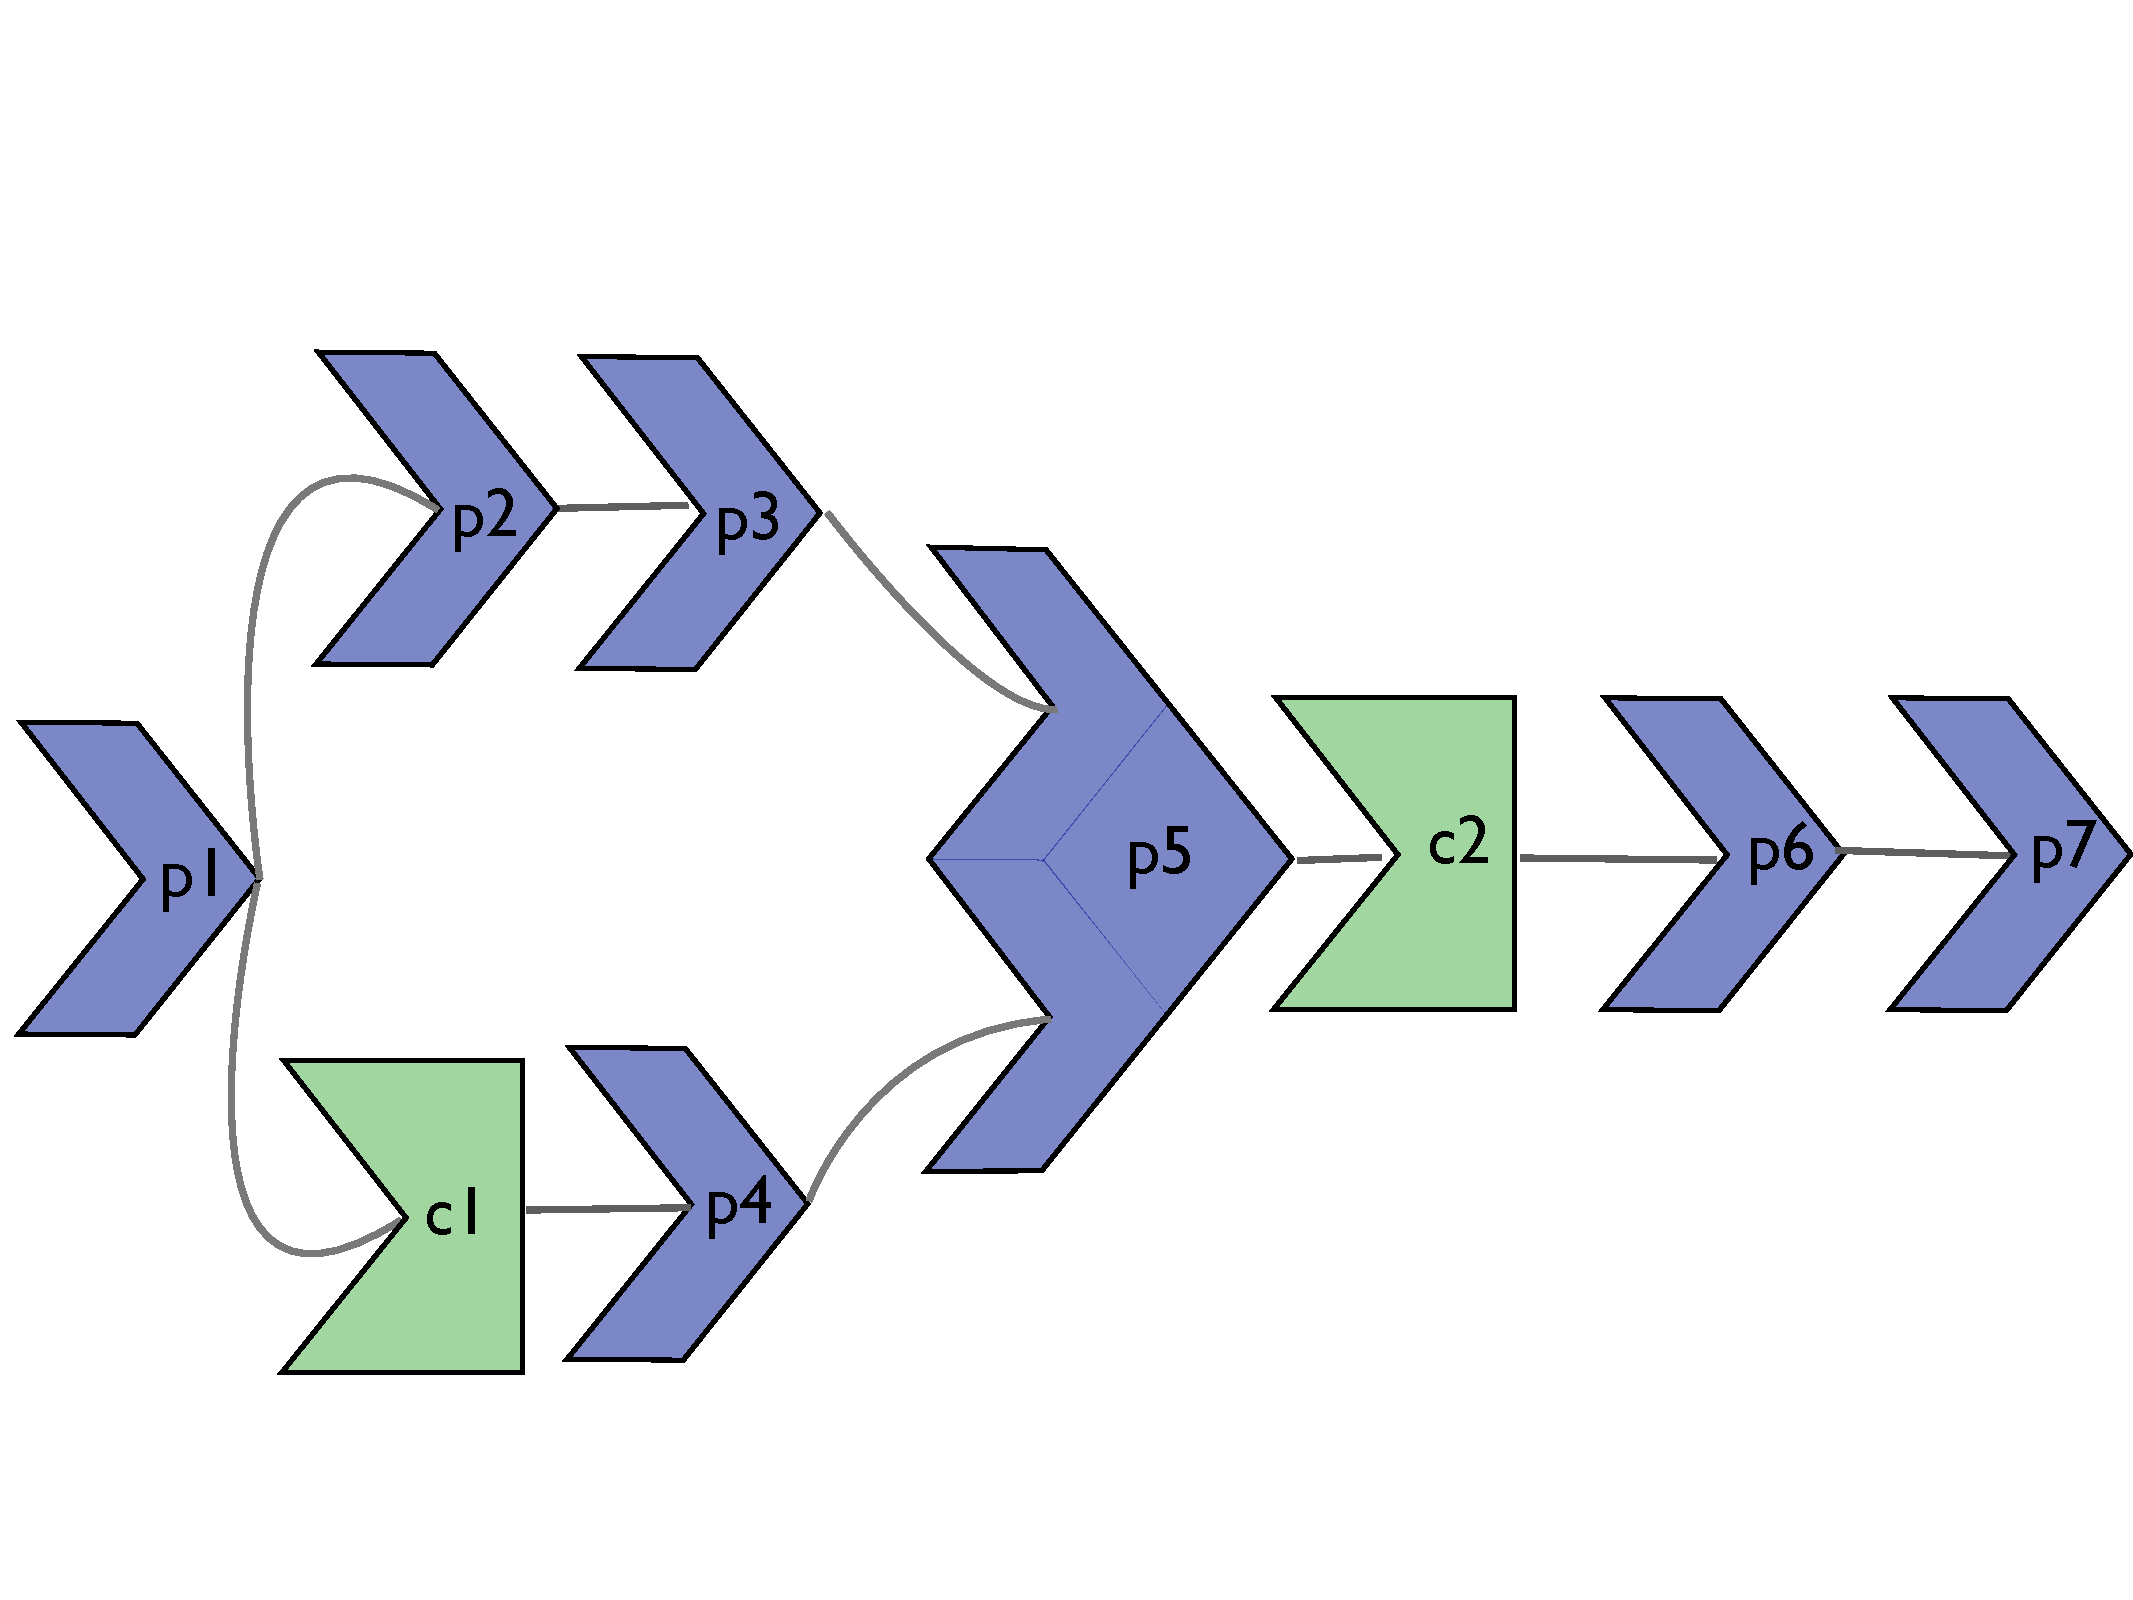
\includegraphics[scale=0.245]{images/opt/fusion1.pdf} \\
    % \flushright \small(After producer/producer fusion)\qquad\\
    \centering  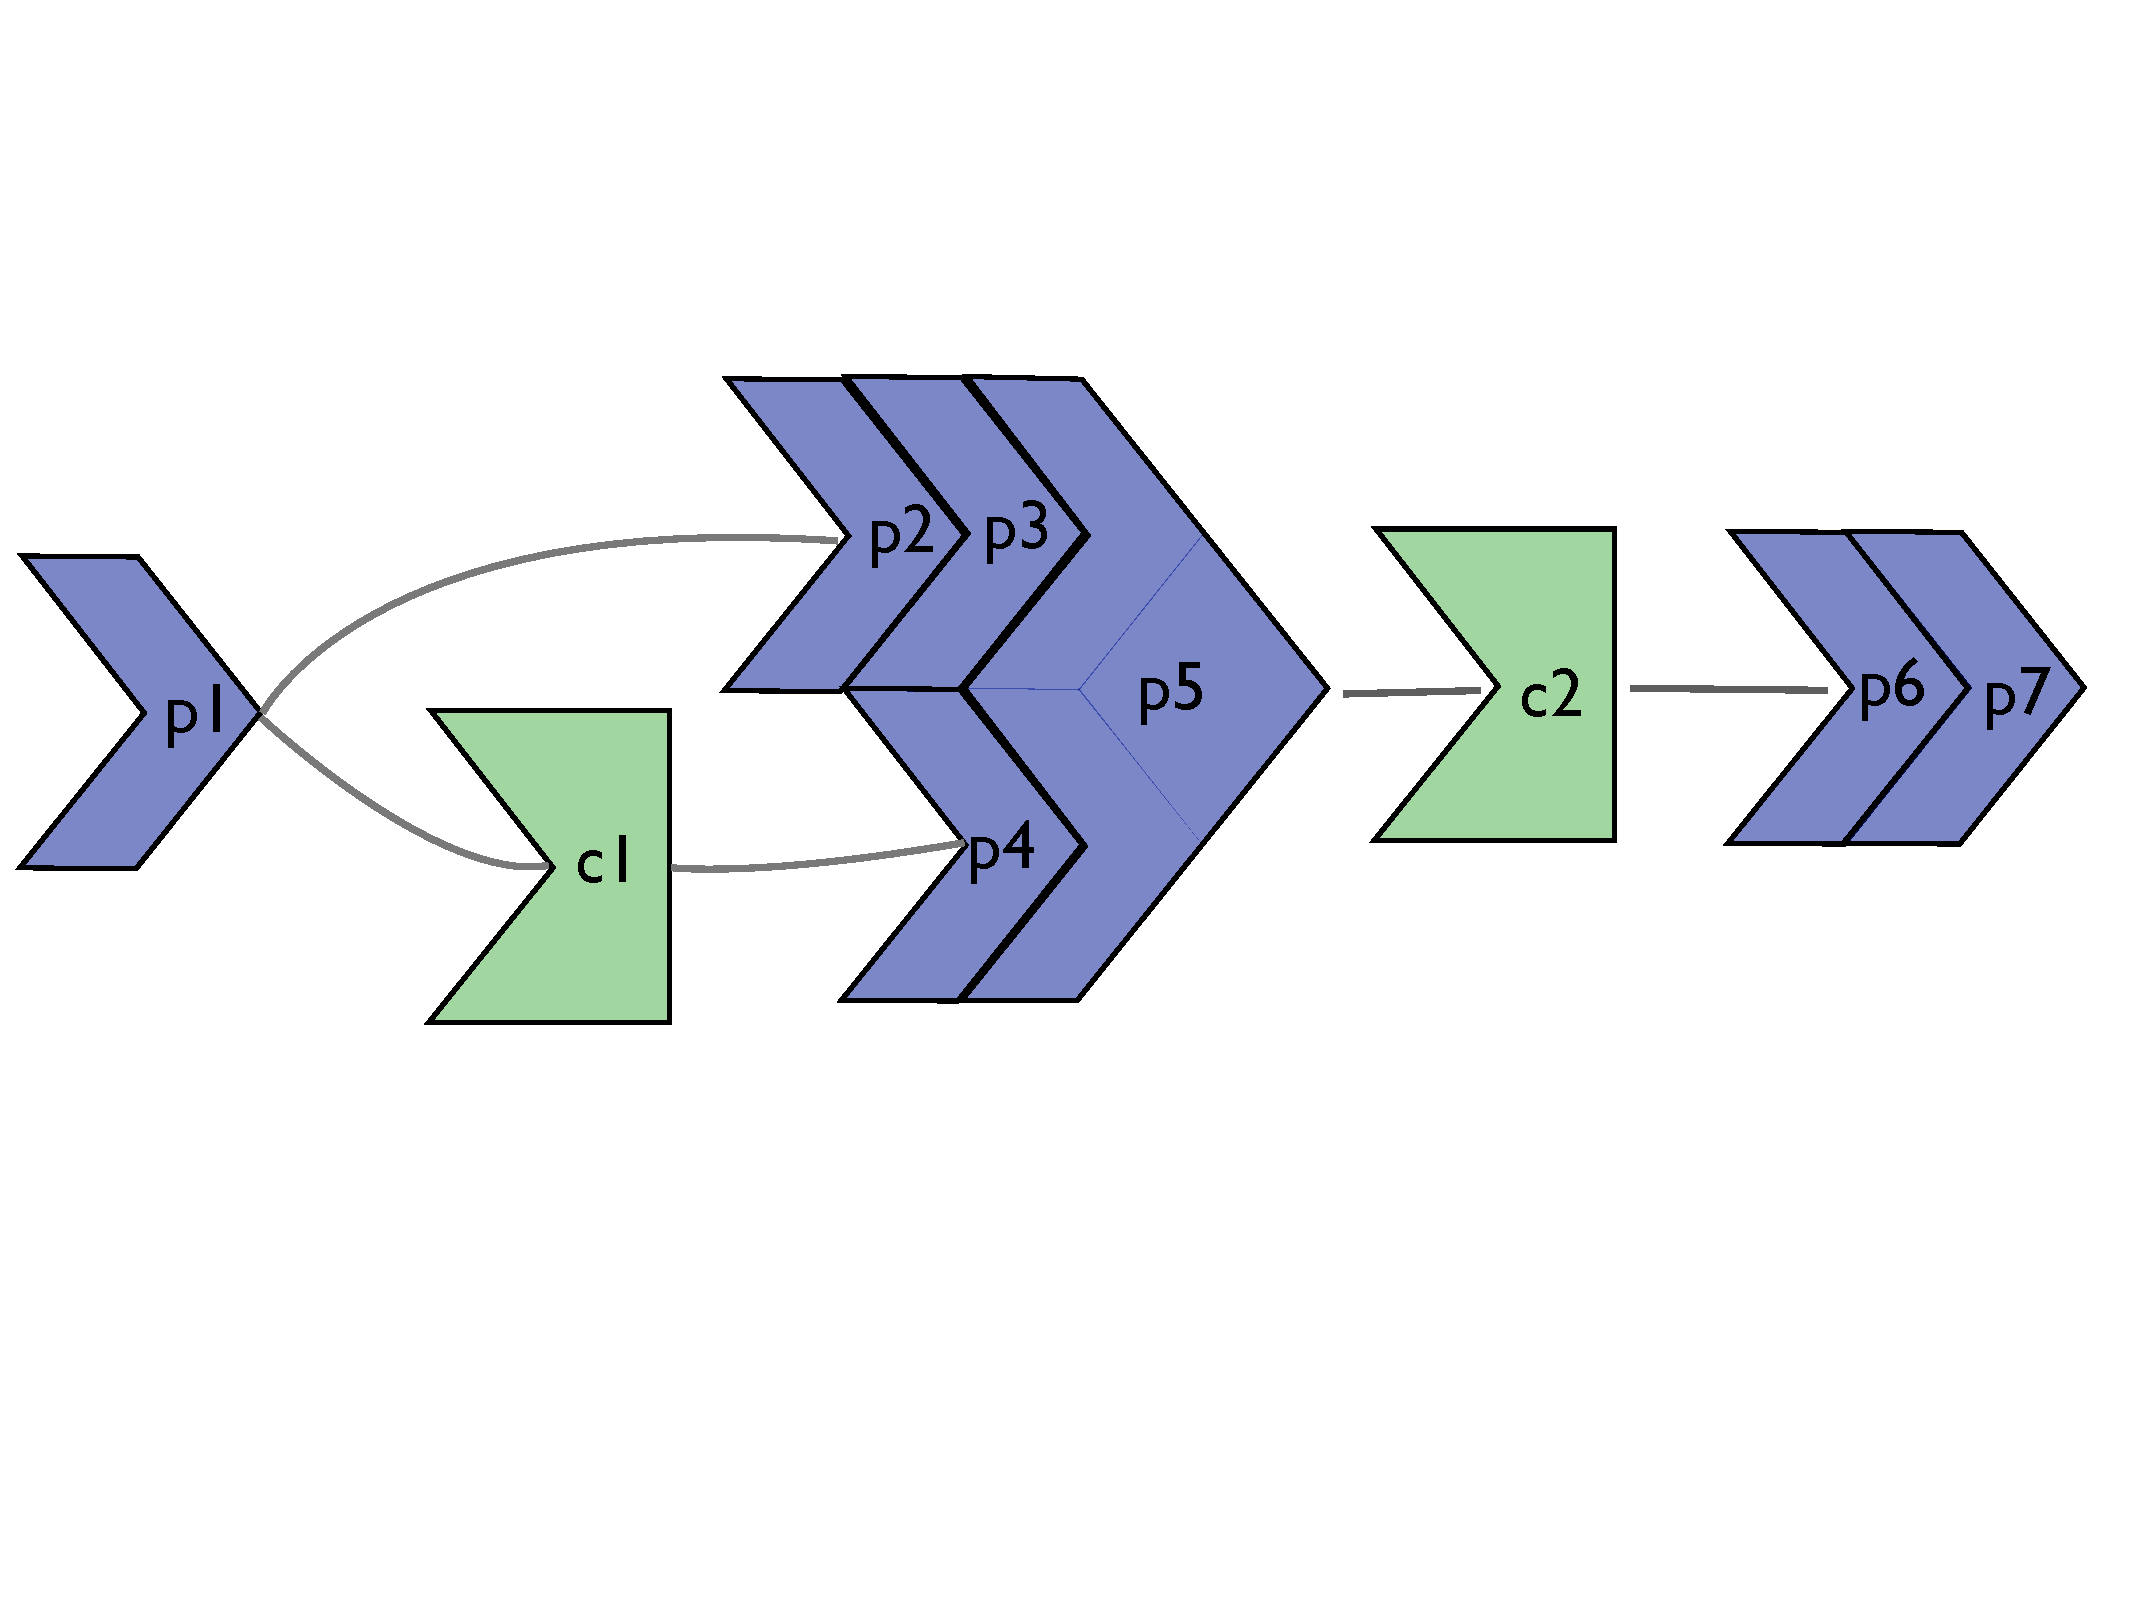
\includegraphics[scale=0.245]{images/opt/fusion2.pdf} \\
    % \flushright \small(After producer/consumer fusion)\qquad\\
    \centering  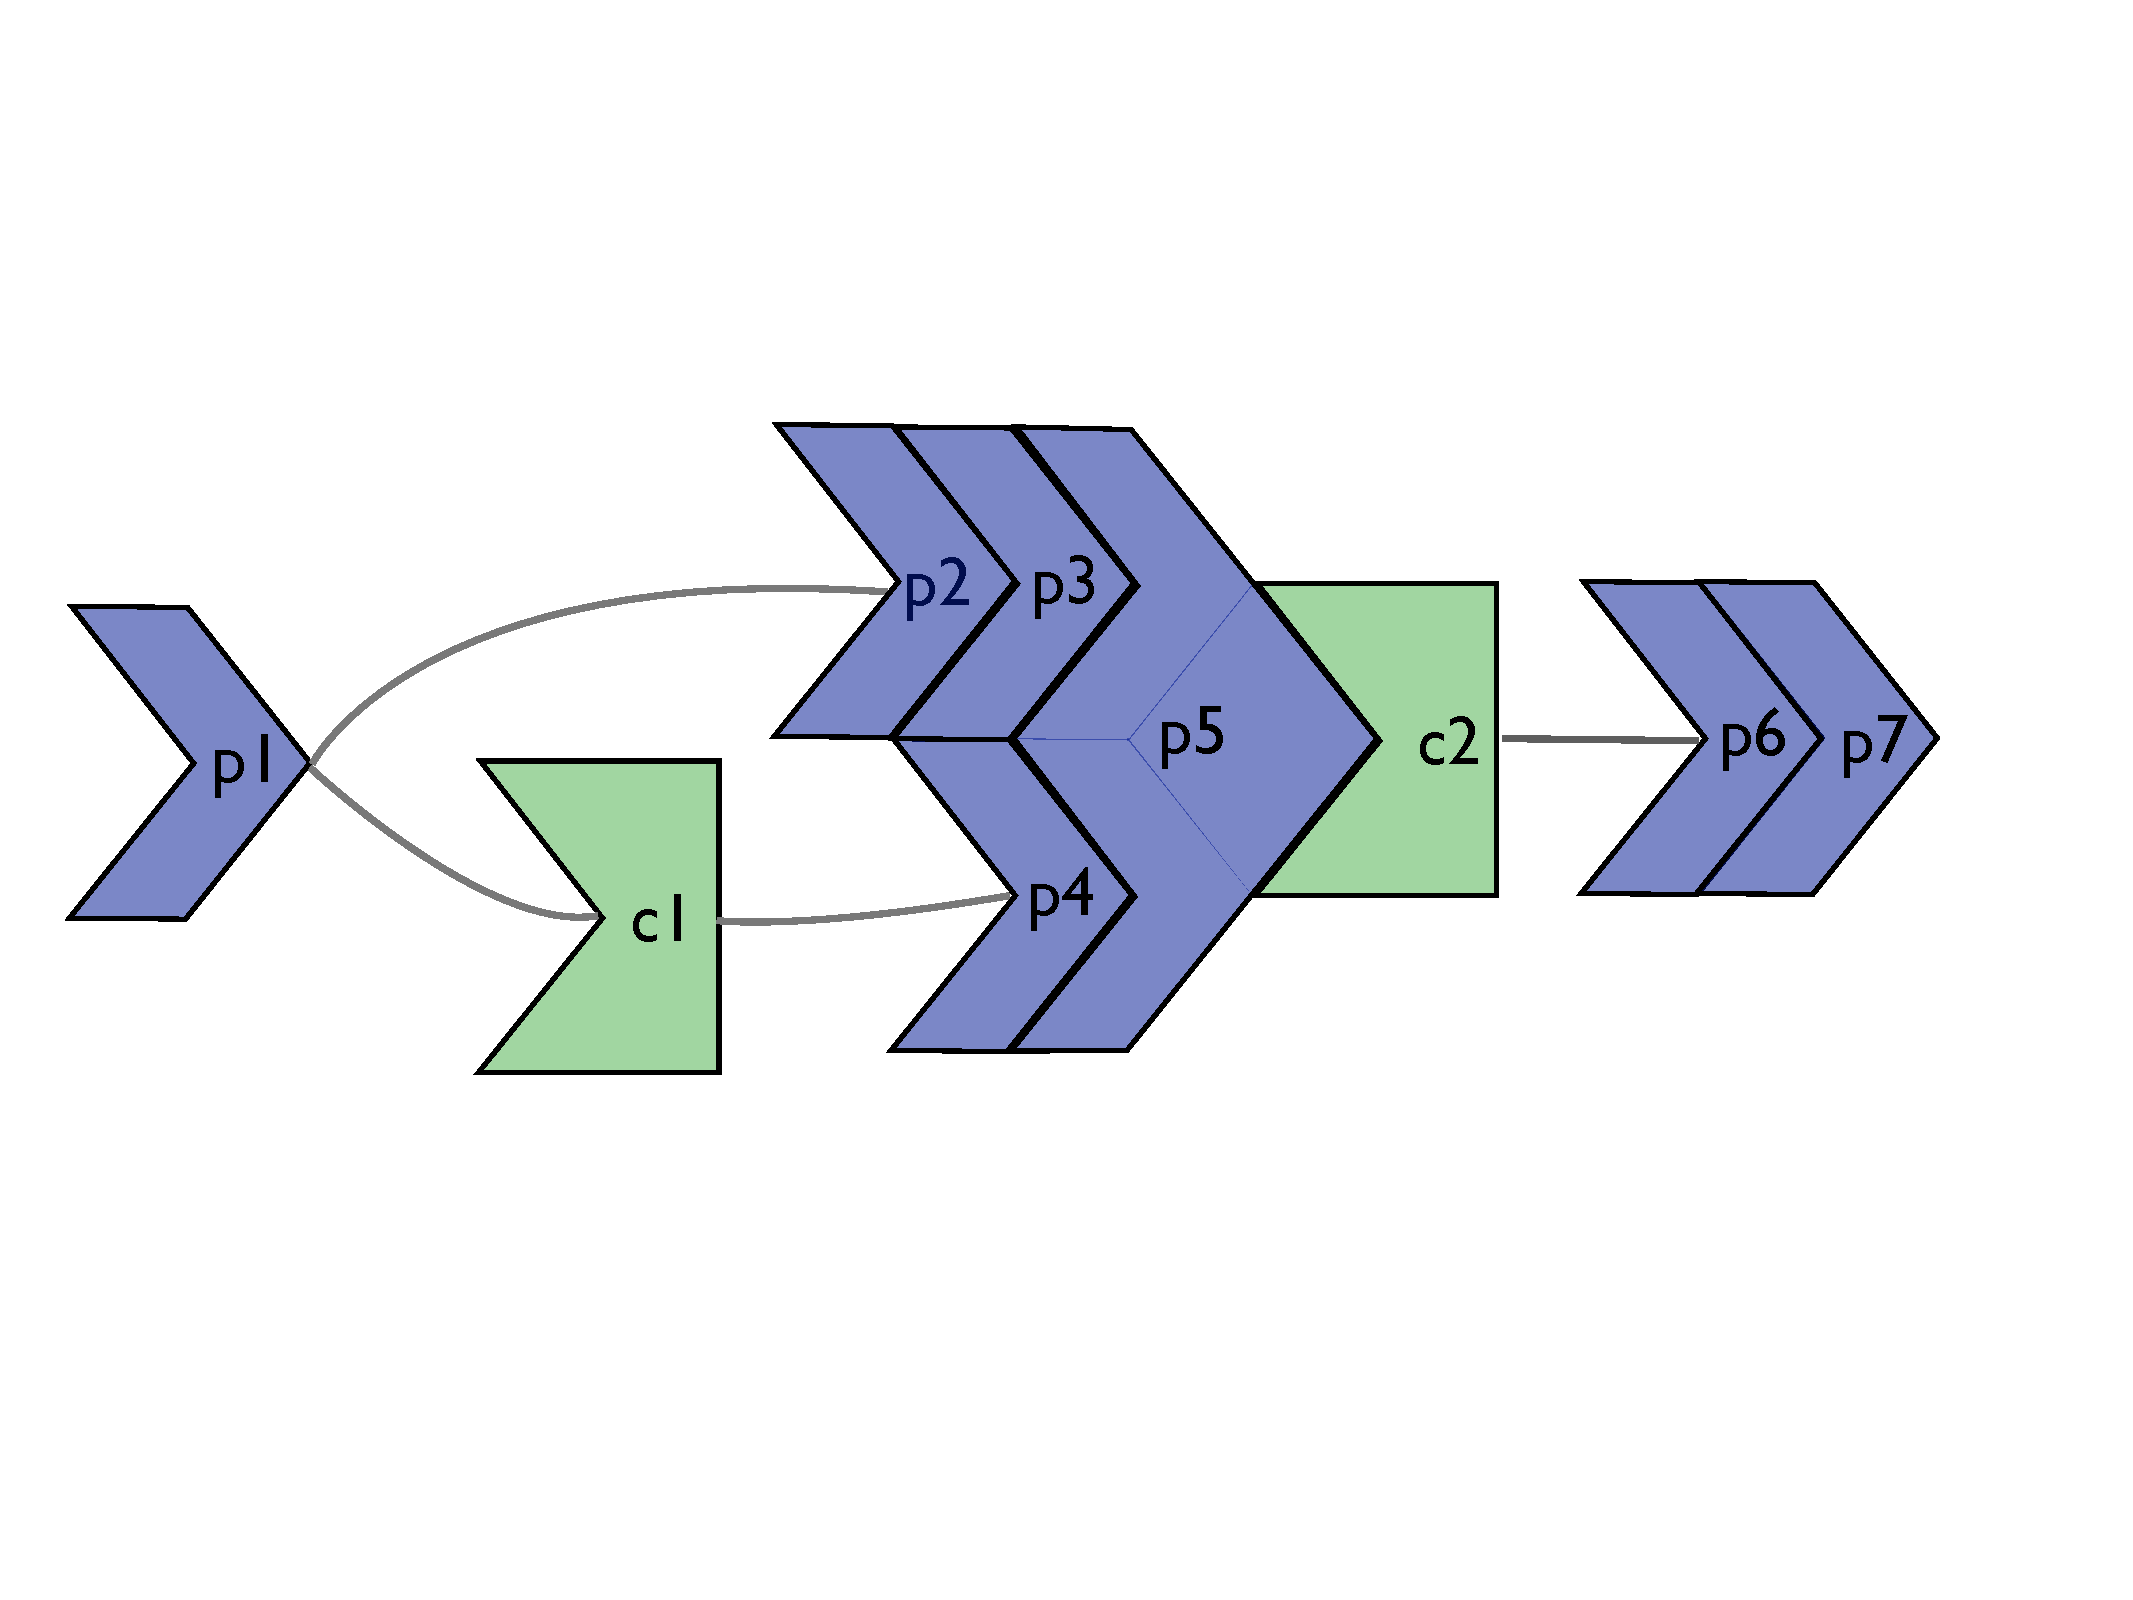
\includegraphics[scale=0.245]{images/opt/fusion3.pdf}
    \caption[Fusion in Accelerate]{The stages of Accelerate's fusion algorithm.
    (1) Before fusion.
    (2) After producer/producer fusion.
    (3) After producer/consumer fusion.}
    \label{fig:fusion}
\end{figure}

Figure~\ref{fig:fusion} shows how the fusion technique affects the
AST: blue boxes labelled $p_1$ to $p_7$ represent
producers, where $p_5$ is a producer like @zipWith@ that takes two arrays as
input. The consumers are labelled $c_1$ and $c_2$. Each box represents an
operation that will be computed to memory, so the goal is to combine the boxes
into the smallest number of clusters as possible.
% In the first phase all adjacent producers are fused, with the exception of
% $p_1$ whose result is used by both $c_1$ and $p_2$. In the second phase, the
% fused producers are embedded into consumers where possible.
In the first phase (centre) successive producer operations are fused together
($p_2$, $p_3$, $p_4$ and $p_5$). In the second phase (bottom) fused producers
are embedded into consumers ($p_{2,3,4,5}$ into $ c_2$). The resulting fused
producer/consumer terms are not fused into successive operations.
%
% In some limited cases it may be possible to fuse $p_{2,3,4,5}/c_2$ into
% $p_{6,7}$, but this is not currently done.
%
Overall, each box in Figure~\ref{fig:fusion} represents a term that will be
computed and stored to memory.

Throughout the transformation $p_1$ is left as is, as its result is used by both
$c_1$ and $p_2$. It would be straightforward to change the implementation such
that the work of $p_1$ is duplicated into both $p_2$ and $c_1$. Despite reducing
memory traffic, this is not always advantageous, so the current implementation
is conservative and never duplicates work. Since Accelerate is a restricted,
deeply embedded language, we can compute accurate cost estimates and make an
informed decision, but this is left for future work. Moreover, this is an
instance of a fundamental limitation with shortcut fusion techniques such as
@foldr/build@~\cite{Gill:1993de} and stream~\cite{Coutts:2007kp} fusion. Since
shortcut fusion is a local transformation that depends on inlining, it is
applicable only to fusing operations which have a single use site. To implement
fusion where an array is efficiently consumed by multiple operations without
work duplication would require fundamental changes to the algorithm.
%
Consumer/producer fusion of $c_1$ into $p_4$, or $c_2$ into $p_6$, would also
require substantial changes to the fusion implementation, and is only applicable
for @map@-like producer terms, as these producers do not require arbitrary array
indexing of the source array.

% \section{Implementing array fusion}
% \label{sec:implementing_array_fusion}

% The current implementation does not fuse the results of consumers
% into subsequent producers ($c_2$ is not fused into $p_{ 6,7 }$), and producers
% used multiple times ($p_1$) are not fused either.
% This has the happy consequence of maintaining trickiest parts of the parallel
% interpretation of the program.

In order to implement the transformation, we require a representation that will
facilitate fusing and embedding producer terms into consumers. We do not wish to
manipulate source terms directly, as this would require a number of rewrite
rules quadratic in the number of operations that are to be fused. This was the
problem with Wadler's original deforestation
algorithm~\cite{Wadler:1981hy,Wadler:1990ix}. The representation must also be
sufficiently expressive to represent all operations we want to fuse, which was a
limitation of @foldr/build@ fusion~\cite{Gill:1993de}.


\subsection{Representing Producers}
\label{sec:representing_producers}

The basic idea behind the representation of producer arrays in Accelerate is
well known: simply represent an array by its size and a function mapping array
indices to their corresponding values. This method has been used successfully to
optimise purely functional array programs in \fusion[delayed array]{}
Repa~\cite{Keller:2010er}, and has also been used by
others~\cite{Claessen:2012hl}.

% The use of delayed arrays in Repa was originally motived by the desire to avoid
% superfluous copying of array elements during index space transformations such as
% @backpermute@ (see Listing~\ref{lst:producer_consumer_operations}).
The major benefit of the use of delayed arrays in Repa is that it offers
by-default automatic fusion. Moreover, this form of fusion does not require
sophisticated compiler transformations or for the two fusible terms to be
statically juxtaposed --- fusion is an inherent property of the data
representation.
%
Automatic fusion sounds too good to be true, and indeed it is. There are at
least two reasons why it is not always beneficial to represent all array terms
uniformly as functions. The first issue is \emph{sharing}. Consider the
following:
%
\begin{lstlisting}[style=haskell]
let b = map f a
in  mmMult b b
\end{lstlisting}
%
Every access to an element @b@ will apply the (arbitrarily expensive) function
@f@ to the corresponding element of @a@. It follows that these computations will
be done \emph{at least twice}, once for each argument of @mmMult@, quite
contrary to the programmer's intent. Indeed, if @mmMult@ consumes its elements
in a non-linear manner, accessing elements more than once, the computation of
@f@ will be performed every time. Thus it is important to be able to represent
some terms as manifest arrays so that a delayed-by-default representation can
not lead to an arbitrary loss of sharing. This is a well known problem with
Repa~\cite{Lippmeier:2012gx}.

The other consideration is \emph{efficiency}. Since we are targeting a massively
parallel architecture designed for performance, it is better to use more
specific operations whenever possible. An opaque indexing function is too
general, conveying no information about the pattern in which the underlying
array is accessed, and hence provides no opportunities for optimisation.

Listing~\ref{lst:Cunctation} shows the ways in which the fusion transformation
represents intermediate arrays. The fusion proceeds by recasting producer array
computations in terms of a set of scalar functions used to construct an element
at each index,
% encoded by this data structure,
and fusing successive producers by combining these scalar functions.
%
\begin{lstlisting}[style=haskell_float
    ,label=lst:Cunctation
    ,caption={Representation of fusible producer arrays}]
data Cunctation acc aenv a where
    Done  :: Arrays arrs                                -- (1)
          => Idx            aenv arrs                   -- manifest array(s)
          -> Cunctation acc aenv arrs

    Yield :: (Shape sh, Elt e)                          -- (2)
          => PreExp     acc aenv sh                     -- output shape
          -> PreFun     acc aenv (sh -> e)              -- compute an element at each index
          -> Cunctation acc aenv (Array sh e)

    Step  :: (Shape sh, Shape sh', Elt a, Elt b)        -- (3)
          => PreExp     acc aenv sh'                    -- output shape
          -> PreFun     acc aenv (sh' -> sh)            -- backwards permutation into input array
          -> PreFun     acc aenv (a   -> b)             -- function to apply to input value
          -> Idx            aenv (Array sh  a)          -- manifest input array
          -> Cunctation acc aenv (Array sh' b)
\end{lstlisting}
%
\makeatchar
The representation\footnote{%
cunc$\cdot$ta$\cdot$tion
\textcolor{gray}{|
k\textipa{`}NGk\textquotesingle t\={a}SH\textipa{`}n \enspace\textipa{k@Nk}\textquotesingle \textipa{te\;IS@n}
% kəNGkˈtāSHən\enspace kəŋkˈteɪʃən
|} (n) the action or an instance of delaying; tardy action.}
\makeatcode
%
is parameterised by the recursive closure of array computations @acc@ and the
array environment @aenv@, and has three constructors:
%
\begin{enumerate}
\item @Done@ injects a manifest array into the type.
    %represented as a reference to a term in the array environment.

\item @Yield@ defines a new array in terms of its shape and a function
    that maps indices to elements.

\item @Step@ encodes a special case of @Yield@, that defines a new
    array by applying an index and value transformation to an argument array.

\end{enumerate}

Note that the argument arrays to @Done@ and @Step@ are not expressed as terms in
@acc@, the type of collective array operations. Instead, requiring a \indext{de
Bruijn} index (@Idx@) into the array environment ensures that the argument array
is manifest. Thus the definition of @Cunctation@ is non-recursive in the type of
array computations. This allows the representation to be embedded within
producer terms (\S\ref{sec:producer_consumer_fusion}) with the guarantee that an
embedded scalar computation will not invoke further parallel computations
(\S\ref{sec:array_computations_vs_scalar_expressions}).
% \footnote{While scalar expression terms are mutually recursive in
% \footcode{acc}, we are guaranteed that these terms will consist only of free
% array variables (\footcode{Idx}).}

In order to bring additional array terms into scope, which may be required for
@Done@ and @Step@, we combine this representation of producer arrays with the
method of Section~\ref{sec:environment_manipulation} for collecting
supplementary environment bindings. Listing~\ref{lst:Embed} shows the complete
data structure used for representing producer terms in Accelerate.
%
\begin{lstlisting}[style=haskell_float
    ,label=lst:Embed
    ,caption={Representation of fused producer arrays}]
data Embed acc aenv a where
    Embed :: Extend     acc aenv aenv'      -- additional bindings to bring into scope, to evaluate the\ldots
          -> Cunctation acc      aenv' a    -- \ldots representation of (fused) producer terms
          -> Embed      acc aenv       a
\end{lstlisting}

Note the types of the array environments in Listing~\ref{lst:Embed}. The @Embed@
type is expressed in relation to the type @aenv@, which represents all
let-bindings currently in scope at this point of the AST that we are analysing.
The data constructor contains an existentially typed @aenv'@. This existential
is witnessed by the first argument @Extend@, that contains any additional array
terms collected during the fusion process
(\S\ref{sec:environment_manipulation}). The delayed array representation in the
second argument is expressed in terms of this extended environment, so has
access to any terms from the AST (@aenv@) as well as those additional bindings
introduced by @Extend@ (@aenv'@).

Why do we separate the auxiliary bindings from the representation of fused
producers? The constructors of @Cunctation@ could carry this information,
and then we would not require this additional data structure. For example, the
following is a valid alternative definition for the @Yield@ constructor:
%
\begin{lstlisting}[style=haskell]
  Yield' :: (Shape sh, Elt e)                   -- Alternative definition (bad)
         => Extend     acc aenv aenv'           -- NEW: supplementary environment bindings
         -> PreExp     acc      aenv' sh        -- CHANGED: inner terms now defined w.r.t. \texttt{aenv'}
         -> PreFun     acc      aenv' (sh -> e)
         -> Cunctation acc aenv       (Array sh e)
\end{lstlisting}

To create a real AST node from the @Embed@ representation, we need both the
environment bindings as well as the array description. However, analysis of how
to fuse terms requires only the array description. If the additional bindings
are bundled as part of the array representation, as in @Yield'@, the
existentially quantified environment type is only available after we pattern
match on the constructor. This is problematic because to inspect terms and do
things like function composition (\S\ref{sec:function_composition}), the types of
the environments of the two terms must be the same. Therefore, after we pattern
match on the constructor we must @sink@ (\S\ref{sec:sinking}) the second term
into @aenv'@. Even worse, for terms in the delayed state the only way to do this
sinking is to first convert them into a real AST node and then back into the
delayed state. If for some reason we can not fuse into this representation ---
for example we do not meet the requirements for the more restrictive @Step@ ---
then this additional work is wasted.

Why can we not analyse terms with respect to the exposed environment type
@aenv@? At some point we will need to merge the extended environments. What
would be the type of this operation? We have no way to express this, even if the
existential types are exposed.
%
\begin{lstlisting}[style=haskell]
cat :: Extend env env1 -> Extend env env2 -> Extend env ???
\end{lstlisting}

Because of the limited scope in which the existential type is available in the
@Yield'@ style representation, we ultimately perform this process of converting
terms and sinking into a suitable type many times. If the extended environments
are placed on the constructors of the delayed representations, the complexity of
the fusion algorithm for an AST of $n$ nodes scales as $\mathcal{O}(r^n)$, where
$r$ is the number of different rules we have for combining delayed terms. While
the semantics of the algorithm are the same, for performance this separation is
critical.

\begin{lstlisting}[style=haskell_float
    ,label=lst:compute
    ,caption={Computing the delayed representation to a manifest array}]
compute :: Arrays arrs => Embed acc aenv arrs -> PreOpenAcc acc aenv arrs
compute (Embed env cc) = bind env (compute' cc)

compute' :: Arrays arrs => Cunctation acc aenv arrs -> PreOpenAcc acc aenv arrs
compute' cc = case simplify cc of
  Done v        -> Avar v                       -- a manifest array
  Yield sh f    -> Generate sh f                -- array from indexing function
  Step sh p f v                                 -- special cases...
    | Just REFL <- match sh (arrayShape v)
    , Just REFL <- isIdentity p
    , Just REFL <- isIdentity f -> Avar v                       -- an unmodified manifest array

    | Just REFL <- match sh (arrayShape v)
    , Just REFL <- isIdentity p -> Map f (avarIn v)             -- linear indexing OK

    | Just REFL <- isIdentity f -> Backpermute sh p (avarIn v)  -- pure index transform

    | otherwise                 -> Transform sh p f (avarIn v)  -- index \& value transform
\end{lstlisting}

Finally, we convert the delayed representations into manifest data using the
@compute@ function shown in Listing~\ref{lst:compute}. It inspects the argument
terms of the representation to identify special cases, such as @map@ and
@backpermute@, as this may allow a backend to emit better code.
%
The helper functions @match@ and @isIdentity@ check for congruence of
expressions. As discussed in Section~\ref{sec:equality}, we match on @Just REFL@
to inject information on the positive case to both the type and value level. For
example, @isIdentity@ checks whether a function corresponds to the term $\lambda
x.x$, and in the positive case witnesses that its type must be @a -> a@.


\subsection{Producer/Producer fusion}
\label{sec:producer_producer_fusion}
\fusion[producer|(]{}

The first phase of the fusion transformation is to merge sequences of producer
functions. Consider the canonical example of map/map fusion, where we would like
to convert the operation @map f (map g xs)@ into the equivalent but more
efficient representation of @map (f . g) xs@, which only makes a single
traversal over the array. While it would be relatively straightforward to
traverse the AST and replace the @map/map@ sequence with the combined
expression, manipulating the source terms directly in this manner requires a
number of rewrite rules quadratic in the number of combinators we wish to fuse.
This approach does not scale.

Instead, producer/producer fusion is achieved by converting terms into the array
representation discussed in Section~\ref{sec:representing_producers}, and
merging sequences of these terms into a single operation. Smart constructors for
each producer manage the integration with predecessor terms. For example,
Listing~\ref{lst:mapD} shows the smart constructor used to generate the fused
version of @map@.

\begin{lstlisting}[style=haskell_float
    ,caption={Smart constructor for fusing the \code{map} operation}
    ,label=lst:mapD]
mapD :: Elt b
     => PreFun     acc aenv (a -> b)
     -> Cunctation acc aenv (Array sh a)
     -> Cunctation acc aenv (Array sh b)
mapD f (step  -> Just (Step sh ix g v)) = Step sh ix (f `compose` g) v
mapD f (yield -> Yield sh g)            = Yield sh (f `compose` g)
\end{lstlisting}

The smart constructor @mapD@ uses two helper functions, @step@ and @yield@, to
expose the only two interesting cases of the delayed representation for this
operation, and compose (\S\ref{sec:function_composition}) the input function @f@
into the appropriate place in the constructor. Index transformation functions
such as @backpermute@ proceed in the same manner. The helper functions @step@
and @yield@ operate by converting the input @Cunctation@ into the constructor of
the same name:
%
\begin{lstlisting}[style=haskell]
step :: Cunctation acc aenv (Array sh e) -> Maybe (Cunctation acc aenv (Array sh e))
step cc = case cc of
  Yield{}                              -> Nothing
  Step{}                               -> Just cc
  Done v | ArraysRarray <- accType' cc -> Just $ Step (arrayShape v) identity identity v

yield :: Cunctation acc aenv (Array sh e) -> Cunctation acc aenv (Array sh e)
yield cc = case cc of
  Yield{}                              -> cc
  Step sh p f v                        -> Yield sh (f `compose` indexArray v `compose` p)
  Done v | ArraysRarray <- accType' cc -> Yield (arrayShape v) (indexArray v)
\end{lstlisting}

A producer such as @map@ can always be expressed as a function from indices to
elements in the style of @Yield@, but this is not the case for the more
restrictive @Step@, which returns a @Maybe Cunctation@. The latter case is used
because we want to keep operations as specific as possible to retain contextual
information, rather than always converting into the most general form of an
indexing function. For the @Done@ case in both instances, GHC can not infer that
the result type is a single @Array@, even though this is specified in the type
signature, so we must use the @accType@ function to reify the @Arrays@ class
representation (ignoring the impossible unmatched cases).

The only producer case that must be handled specially is  that of @zipWith@, as
this is the only producer which consumes multiple arrays (see
Listing~\ref{lst:producer_consumer_operations}). In contrast to, for example,
@foldr/build@, we are able to fuse the operation in
both of the input arguments. The @zipWith@ smart constructor is shown in
Listing~\ref{lst:zipWithD}. We note the following characteristics:
%
\begin{enumerate}
\item Because it is advantageous to express operations in the most specific way
    possible, @zipWith@ considers the special case of when the two input arrays
    derive from the same manifest source data with the same indexing pattern.

\item The default behaviour is to convert both input arrays into functions from
    indices to elements, and @combine@ these into a single indexing function.

\item The function @combine@ completes the task of drawing an element from each
    of the input arrays and combining them with the binary function @f@, being
    sure to let-bind the intermediate results along the way.

\item The first guard requires a type signature, otherwise the type variable @e@
    introduced by the weakening step will ``escape'', and can not be unified
    correctly. This new parameter @e@ represents for (1) the array element type,
    and at (2) the array index type.

\end{enumerate}

\begin{lstlisting}[style=haskell_float
    ,name=zipWithD
    ,label=lst:zipWithD
    ,caption={Smart constructor for fusing the \code{zipWith} operation}]
zipWithD :: (Shape sh, Elt a, Elt b, Elt c)
         => PreFun     acc aenv (a -> b -> c)
         -> Cunctation acc aenv (Array sh a)
         -> Cunctation acc aenv (Array sh b)
         -> Cunctation acc aenv (Array sh c)
zipWithD f cc1 cc0
  | Just (Step sh1 p1 f1 v1)    <- step cc1
  , Just (Step sh0 p0 f0 v0)    <- step cc0
  , Just REFL                   <- match v1 v0
  , Just REFL                   <- match p1 p0
  = Step (sh1 `Intersect` sh0) p0 (combine f f1 f0) v0                                 -- (1)

  | Yield sh1 f1                <- yield cc1
  , Yield sh0 f0                <- yield cc0
  = Yield (sh1 `Intersect` sh0) (combine f f1 f0)                                      -- (2)
  where
    combine :: forall acc aenv a b c e. (Elt a, Elt b, Elt c)
            => PreFun acc aenv (a -> b -> c)
            -> PreFun acc aenv (e -> a)
            -> PreFun acc aenv (e -> b)
            -> PreFun acc aenv (e -> c)
    combine c ixa ixb                                                                  -- (3)
      | Lam (Lam (Body c')) <- weakenFE SuccIdx c                                      -- (4)
                                        :: PreOpenFun acc ((),e) aenv (a->b->c)
      , Lam (Body ixa')     <- ixa
      , Lam (Body ixb')     <- ixb
      = Lam $ Body $ Let ixa' $ Let (weakenE SuccIdx ixb') c'
\end{lstlisting}

The first phase of fusion can now be completed via bottom-up tree contraction of
the AST\@. Smart constructors for each of the producer functions are used to
convert terms into the intermediate representation, and adjacent
producer/producer terms are merged. Listing~\ref{lst:embedPreAcc} demonstrates
the procedure.
%
\begin{lstlisting}[style=haskell_float
    ,label=lst:embedPreAcc
    ,caption={Producer fusion via bottom-up contraction of the AST}]
embedPreAcc
    :: forall acc aenv arrs. Arrays arrs
    => PreOpenAcc acc aenv arrs
    -> Embed      acc aenv arrs
embedPreAcc pacc =
  case pacc of
    Alet bnd body       -> aletD bnd body                                              -- (1)
    Use arrs            -> done  (Use arrs)                                            -- (2)

    Map f a             -> fuse  (into  mapD     (cvtF f)) a                           -- (3)
    ZipWith f a b       -> fuse2 (into  zipWithD (cvtF f)) a b

    Fold f z a          -> embed (into2 Fold     (cvtF f) (cvtE z)) a                  -- (4)
    ...
  where
    done :: Arrays a => PreOpenAcc acc aenv a -> Embed acc aenv a
    done (Avar v) = Embed BaseEnv                  (Done v)
    done pacc     = Embed (BaseEnv `PushEnv` pacc) (Done ZeroIdx)

    into :: Sink f => (f env' a -> b) -> f env a -> Extend acc env env' -> b
    into op a env = op (sink env a)

    fuse :: Arrays as
         => (forall aenv'. Extend acc aenv aenv'
                       -> Cunctation acc aenv' as
                       -> Cunctation acc aenv' bs)
         ->       acc aenv as
         -> Embed acc aenv bs
    fuse op (embedAcc -> Embed env cc) = Embed env (op env cc)

    embed :: (Arrays as, Arrays bs)
          => (forall aenv'. Extend acc aenv aenv'
                        ->            acc aenv' as
                        -> PreOpenAcc acc aenv' bs)
          ->       acc aenv as
          -> Embed acc aenv bs
    embed op (embedAcc -> Embed env cc)
      = Embed (env `PushEnv` op env (injectAcc (compute' cc))) (Done ZeroIdx)

injectAcc :: PreOpenAcc acc aenv a -> acc aenv a
embedAcc  :: Arrays arrs => acc aenv arrs -> Embed acc aenv arrs
\end{lstlisting}

\begin{enumerate}
\item Non-computation forms such as control flow and let bindings may also
    employ smart constructors. We discuss fusion of let bindings in
    Section~\ref{sec:binder_elimination}.

\item Array introduction forms convert their argument into the internal
    representation by adding the term as manifest data into the extended
    environment. This also illustrates why we require both @Done@ and @Step@
    constructors in the delayed representation (Listing~\ref{lst:Cunctation}).
    It would be convenient to represent manifest data as a @Step@ node with
    identity transformation functions, but the type of @Step@ is restricted to a
    single @Array@, whereas @Done@ is generalised to the @Arrays@ class.

\item Producer terms such as @map@ and @zipWith@ are converted into the internal
    representation (Listing~\ref{lst:Cunctation}) using their smart
    constructors. In order to do this, all terms must be defined with respect to
    the same environment type. The helper function @fuse@ encodes the bottom-up
    traversal by first converting the argument array @a@ into the @Embed@
    representation. The extended environment type and delayed representation are
    then passed to the continuation function @into@, which sinks
    (\S\ref{sec:environment_manipulation}) the argument @f@ into the extended
    environment type of the delayed representation, before applying the smart
    constructor @mapD@ (Listing~\ref{lst:mapD}). This results into a new delayed
    representation that can be further fused into later terms. At the @zipWith@
    case @fuse2@ acts analogously, but must ensure that the two input array
    terms are lowered into the same extended environment.

\item Consumer operations such as @fold@ force the operation to be evaluated to
    a manifest array at this point in the program, by converting the @Embed@
    representation back into AST terms using @compute'@
    (Listing~\ref{lst:compute}) and pushing the result onto the extended
    environment. Consumers fusion will be treated in
    Section~\ref{sec:producer_consumer_fusion}, although note that the producer
    is placed adjacent to the term that consumes it.

\end{enumerate}

The result of this process is an AST where all adjacent producer/producer
operations have been combined into a single producer. The next step of the
fusion pipeline is to fuse producers into consumers.

\fusion[producer|)]{}

\subsection{Producer/Consumer fusion}
\label{sec:producer_consumer_fusion}
\fusion[consumer|(]{}

Now that we have a story for producer/producer fusion, we discuss how to deal
with consumers. Recall the classic array fusion example that is vector dot
product:

\begin{lstlisting}[style=haskell]
dotp :: Acc (Vector Float) -> Acc (Vector Float) -> Acc (Scalar Float)
dotp xs ys = A.fold (+) 0                       -- sum result of\ldots
           $ A.zipWith (*) xs ys                -- \ldots element-wise multiplying inputs
\end{lstlisting}
%
This consists of two collective operations: the first multiplies values from the
two input arrays element-wise, and the second sums this result. The fusion
system should translate this into a single collective operation, in much the
same way as a human would write if working directly in a low-level language such
as C or CUDA\@.

For the dot product example, the delayed producer is equivalent to the scalar
function @\ix -> (xs!ix) * (ys!ix)@. This function must be embedded directly
into the implementation for @fold@ so that the values are generated online,
without an intermediate array. However, these two steps happen at different
phases of the compilation pipeline: producers are fused using smart
constructors, as described in the previous section, but producers are only
finally embedded into consumers during code
generation~(\S\ref{sec:code_generation}).

To work around this stage mismatch, the second phase of the fusion
transformation annotates the program AST (see Section~\ref{sec:knot_tying}) with
the representation shown in Listing~\ref{lst:DelayedOpenAcc}. This encodes the
information as to which nodes should be computed to manifest arrays, and which
should be embedded into their consumers. During code generation, the code for
the embedded producer terms, such as @indexD@, is generated and integrated
directly into the skeleton for the consumer
(\S\ref{sec:instantiating_skeletons}). The end result is that no intermediate
array needs to be created.

\begin{lstlisting}[style=haskell_float
    ,name=DelayedOpenAcc
    ,label=lst:DelayedOpenAcc
    ,caption={Representation of delayed arrays}]
data DelayedOpenAcc aenv a where
  Manifest              :: PreOpenAcc DelayedOpenAcc aenv a
                        -> DelayedOpenAcc aenv a

  Delayed               :: (Shape sh, Elt e) =>
    { extentD           :: PreExp DelayedOpenAcc aenv sh
    , indexD            :: PreFun DelayedOpenAcc aenv (sh  -> e)
    , linearIndexD      :: PreFun DelayedOpenAcc aenv (Int -> e)
    }                   -> DelayedOpenAcc aenv (Array sh e)
\end{lstlisting}

The second phase of fusion is implemented as a top-down translation of the
@Embed@ representation from the first phase
(\S\ref{sec:producer_producer_fusion}) into an AST that uses @DelayedOpenAcc@ to
make the representation of fused producer/consumer pairs explicit. This
procedure, shown in Listing~\ref{lst:convertOpenAcc}, has the following points
of note:

\begin{lstlisting}[style=haskell_float,
    label=lst:convertOpenAcc,
    caption={Consumer fusion via top-down annotation of the AST}]
convertOpenAcc
    :: Arrays arrs
    =>        OpenAcc aenv arrs
    -> DelayedOpenAcc aenv arrs
convertOpenAcc = manifest . computeOpenAcc . embedOpenAcc                              -- (1)
  where
    manifest :: OpenAcc aenv a -> DelayedOpenAcc aenv a
    manifest (OpenAcc pacc) =
      Manifest $ case pacc of                                                          -- (2)
        Use arr         -> Use arr
        Alet a b        -> alet (manifest a) (manifest b)                              -- (3)
        Map f a         -> Map  (cvtF f) (delayed a)
        Fold f z a      -> Fold (cvtF f) (cvtE z) (delayed a)                          -- (4)
        Stencil f b a   -> Stencil (cvtF f) b (manifest a)                             -- (5)
        ...

    delayed :: (Shape sh, Elt e)
            => OpenAcc        aenv (Array sh e)
            -> DelayedOpenAcc aenv (Array sh e)
    delayed (embedOpenAcc fuseAcc -> Embed BaseEnv cc) =                               -- (6)
      case cc of
        Done v          -> Delayed (arrayShape v) (indexArray v) (linearIndex v)
        ...

    cvtF :: OpenFun env aenv f -> DelayedOpenFun env aenv f
    cvtE :: OpenExp env aenv t -> DelayedOpenExp env aenv t
\end{lstlisting}
% embedOpenAcc   :: Arrays arrs => OpenAcc aenv arrs -> Embed OpenAcc aenv arrs
% computeOpenAcc :: Arrays arrs => Embed OpenAcc aenv aenv arrs -> OpenAcc aenv arrs


\begin{enumerate}
\item The fusion pipeline proceeds in two phases. A bottom-up traversal that
    merges adjacent producer/producer pairs, which is implemented by the
    function @embedOpenAcc@, described in
    Section~\ref{sec:producer_producer_fusion}. The second phase is the top-down
    traversal which annotates the AST as to which nodes should be computed to
    manifest data and which should be embedded into their consumers. This phase
    is implemented by the function @manifest@.

\item For the most part, the function @manifest@ simply wraps each node of the
    AST in the @Manifest@ constructor, indicating that this term should be
    computed to memory.

\item Similarly, let bindings compute both the binding and body to manifest
    arrays. The smart constructor @alet@ flattens needless let bindings of the
    form @let var = x in var@ to @x@. This form is common, as the delayed array
    constructors always refer to manifest data via de Bruijn indices (see
    Listing~\ref{lst:Cunctation}), meaning that all manifest terms will be let
    bound regardless of the number of use sites.

\item A consumer such as @fold@ specifies that its array valued argument should
    be @delayed@, so the representation of producer terms is used to annotate
    the AST node directly. Code generation will later embed this functional
    representation directly into the consumer skeleton, thereby completing the
    producer/consumer fusion process
    (\S\ref{sec:fusion_by_template_instantiation}).

\item In contrast, stencil operations (\S\ref{sec:parallel_stencil}) --- where
    the computation of each element has access to elements within a local
    neighbourhood --- first fully computes the argument to a manifest array in
    order to avoid duplicating the work of the delayed representation at each
    array access. The transformation thus makes it clear for which operations
    the argument arrays will be delayed, and for which operations the arguments
    are manifest.

\item The function @delayed@ generates the delayed array representation of how
    to produce each array element that can be directly embedded into consumers.
    The function takes care to recover optimisation opportunities such as linear
    indexing of the underlying array data. Note that it is safe to match on
    @BaseEnv@ --- indicating no additional terms are being brought into scope
    --- because the first phase always places producers adjacent to the term
    that will consume it; see the definition of @embed@ in
    Listing~\ref{lst:embedPreAcc}.

\end{enumerate}

Overall, adjacent producer/producer pairs have been merged, and consumers can
integrate directly into the skeleton the code for on-the-fly producing each
element so that no intermediate array needs to be created.

\fusion[consumer|)]{}

\subsection{Exploiting all opportunities for fusion}
\label{sec:binder_elimination}

The approach to array fusion employed by Accelerate is similar to that used by
Repa~\cite{Keller:2010er,Lippmeier:2011cd,Lippmeier:2012gx}, although the idea
of representing arrays as functions is well known~\cite{Guibas:1978jh,Elliott:2003ug}. It was discovered that one of
the most immediately pressing problems with delayed arrays in Repa was that it
did not preserve sharing. In Repa, the conversion between delayed and manifest
arrays is done manually, where by default shared expressions will be recomputed
rather than stored. Depending on the algorithm, such recomputation can be
beneficial, but excessive recomputation quickly ruins performance.

However, since Accelerate has explicit sharing information encoded in the term
tree as let bindings, we can avoid the problem of unrestrained inlining that can
be a problem when using Repa. While we want to be careful about fusing
shared array computations to avoid duplicating work, \emph{scalar} Accelerate
computations that manipulate \emph{array shapes}, as opposed to the bulk array
data, can lead to terms that employ sharing but can never duplicate work. Such
terms are common in Accelerate code and so it is important that they are treated
specially so that they do not inhibit fusion.


\subsubsection{let-elimination}

Consider the following example that first reverses a vector with @backpermute@,
and then maps a function @f@ over the result. Being a function of two producer
term (see Listing~\ref{lst:producer_consumer_operations}) we would hope these
are fused into a single operation:%
% \footnote{Some details of the backwards permutation function are elided for
% clarity. See the definition of \texttt{reverse}:
% \url{http://hackage.haskell.org/packages/archive/accelerate/latest/doc/html/Data-Array-Accelerate.html\#v:reverse}}
%
\begin{lstlisting}[style=haskell]
reverseMap f xs
  = map f
  $ backpermute (shape xs) (ilift1 $ \i -> length xs - i - 1) xs
\end{lstlisting}
%
Unfortunately, sharing recovery, using the algorithm from
Section~\ref{sec:sharing_recovery}, causes a problem. The variable @xs@
is used three times in the arguments to @backpermute@, so sharing recovery
introduces a let binding at the lowest common meet point for all uses of the
array. This places it between the @map@ and @backpermute@ operations:
%
\begin{lstlisting}[style=haskell]
reverseMap f xs
  = map f
  $ let v = xs
    in  backpermute (shape v) (\i -> length v - i - 1) v
\end{lstlisting}
%
The binding, although trivial, prevents fusion of the two producer terms.
Moreover, it does so unnecessarily. The argument array is used three times:
twice to access shape information, but only once to access the array data ---
in the final argument to @backpermute@.

Fortunately there is a simple workaround. Since the delayed array constructors
representing producer arrays, @Step@ and @Yield@ (Listing~\ref{lst:Cunctation}),
carry the shape of the arrays they represent as part of the constructor, we can
disregard all uses of the array that only access shape information. For this
example, that leaves us with just a single reference to the array's payload.
That single reference allows us remove the unnecessary let-binding and re-enable
fusion.

Let-elimination can also be used to \emph{introduce} work duplication, which may
be beneficial if we can estimate that the cost of the recomputation is less than
the cost of completely evaluating the array to memory and subsequently
retrieving the values. While Accelerate is currently conservative and never
introduces work duplication, since we have the entire term tree available, we
could compute an accurate cost model and make an informed decision. Such
analysis is left to future work.


\subsubsection{let-floating}

Similarly, the semantics of our program do not change if we float let bindings
of manifest data across producer chains. This helps to expose further
opportunities for producer/producer fusion. For example, we can allow the
binding of @xs@ to floating above the @map@ so that the two producers can be
fused:
%
\begin{lstlisting}[style=haskell]
map g $ let xs = use (Array ...)
        in zipWith f xs xs
\end{lstlisting}
%
While floating let bindings opens up the potential for further optimisations, we
must be careful to not change the \emph{scope} of let bindings, as that would
increase the lifetime of bound variables, and hence increase live memory usage.


\par{} %\subsubsection{Smart constructor for let bindings}

Both these tasks, let-floating and let-elimination, are handled by a smart
constructor for let bindings during the first fusion phase that contracts the
AST and merges adjacent producer/producer pairs
(\S\ref{sec:producer_producer_fusion}). The smart constructor for let bindings
must consider several cases, as well as maintain type correctness and the
complexity of the algorithm, by ensuring each term is inspected exactly once.
The code is shown in Listing~\ref{lst:aletD}.

\begin{lstlisting}[style=haskell_float
    ,label=lst:aletD
    ,caption={Smart constructor for let bindings}]
type ElimAcc  acc = forall aenv s t. acc aenv s -> acc (aenv,s) t -> Bool

aletD :: (Arrays arrs, Arrays brrs)
      => ElimAcc acc
      ->       acc aenv        arrs
      ->       acc (aenv,arrs) brrs
      -> Embed acc aenv        brrs
aletD elimAcc (embedAcc -> Embed env1 cc1) acc0
  | Done v1             <- cc1                                                         -- (1)
  , Embed env0 cc0      <- embedAcc $ rebuildAcc (subAtop (Avar v1) . sink1 env1) acc0
  = Embed (env1 `append` env0) cc0

  | otherwise                                                                          -- (2)
  = aletD' elimAcc (Embed env1 cc1) (embedAcc acc0)


aletD' :: forall acc aenv arrs brrs. (Arrays arrs, Arrays brrs)
       => ElimAcc acc
       -> Embed acc aenv         arrs
       -> Embed acc (aenv, arrs) brrs
       -> Embed acc aenv         brrs
aletD' elimAcc (Embed env1 cc1) (Embed env0 cc0)
  | acc1                <- compute (Embed env1 cc1)                                    -- (3)
  , False               <- elimAcc (inject acc1) acc0
  = Embed (BaseEnv `PushEnv` acc1 `append` env0) cc0

  | acc0'               <- sink1 env1 acc0                                             -- (4)
  = case cc1 of
      Step{}    -> eliminate env1 cc1 acc0'
      Yield{}   -> eliminate env1 cc1 acc0'

  where
    acc0 :: acc (aenv, arrs) brrs
    acc0 = computeAcc (Embed env0 cc0)

    eliminate :: forall aenv aenv' sh e brrs. (Shape sh, Elt e, Arrays brrs)                -- (5)
              => Extend     acc aenv aenv'
              -> Cunctation acc      aenv' (Array sh e)
              ->            acc     (aenv', Array sh e) brrs
              -> Embed      acc aenv                    brrs
    eliminate env1 cc1 body
      | Done v1           <- cc1 = elim (arrayShape v1) (indexArray v1)
      | Step sh1 p1 f1 v1 <- cc1 = elim sh1 (f1 `compose` indexArray v1 `compose` p1)
      | Yield sh1 f1      <- cc1 = elim sh1 f1
      where
        bnd :: PreOpenAcc acc aenv' (Array sh e)
        bnd = compute' cc1

        elim :: PreExp acc aenv' sh -> PreFun acc aenv' (sh -> e) -> Embed acc aenv brrs
        elim sh1 f1
          | sh1'                <- weakenEA rebuildAcc SuccIdx sh1
          , f1'                 <- weakenFA rebuildAcc SuccIdx f1
          , Embed env0' cc0'    <- embedAcc                                            -- (8)
                                    $ rebuildAcc (subAtop bnd)                         -- (7)
                                    $ replaceAcc sh1' f1' ZeroIdx body                 -- (6)
          = Embed (env1 `append` env0') cc0'

    replaceAcc :: forall aenv sh e a. (Shape sh, Elt e)
               => PreExp acc aenv sh -> PreFun acc aenv (sh -> e) -> Idx aenv (Array sh e)
               -> acc aenv a
               -> acc aenv a

subAtop :: Arrays t => PreOpenAcc acc aenv s -> Idx (aenv, s) t -> PreOpenAcc acc aenv t
sink1   :: Sink f => Extend acc env env' -> f (env, s) t -> f (env', s) t
\end{lstlisting}

\begin{enumerate}
\item If the binding is a manifest array, immediately inline the variable
    referring to the bound expression into the body, instead of adding the
    binding to the environment and thereby creating an indirection that must be
    later eliminated. This effectively floats let-bound terms across
    producer-producer chains.

\item Note that on entry to the @aletD@ smart constructor, the binding term is
    converted to the internal representation (via the view pattern), but the
    body expression is left as is. This is important, as the inlining process in
    (1) can only be applied to \emph{concrete} AST terms, not to the delayed
    @Embed@ representation. Only if the binding is not a manifest term do we
    convert the body to the delayed representation in order to analyse it. This
    ensures the body is only traversed once, maintaining complexity of the
    algorithm. The subsequent cases, where we wish to analyse both the binding
    and body expressions in delayed form, is handled by the auxiliary function
    @aletD'@.

\item The first case checks whether it is possible to eliminate the let binding
    at all, using the continuation @elimAcc@. The implementation of this
    function is shown in Listing~\ref{lst:elimAcc}. Note that the analysis must
    be applied to the binding @cc1@ plus its local environment @env1@, otherwise
    we can be left with dead terms that are not subsequently eliminated.

    If the let binding will not be eliminated, it is added to the extended
    environment, indicating that it is to be evaluated to a manifest term. Note
    that it is important to add the term to a \emph{new} environment. Otherwise,
    nested let bindings are effectively flattened, resulting in terms required
    for the bound term being lifted out into the same scope as the body. That
    is, if we don't place the binding into a fresh environment, we get terms
    such as:
    %
\begin{lstlisting}[style=haskell]
let a0  = %$\langle$ terms for binding $\rangle$% in
let bnd = %$\langle$ bound term $\rangle$% in
%$\langle$ body term $\rangle$%
\end{lstlisting}
    %
    Rather than the following, where the scope of @a0@ is restricted to the
    evaluation of the bound term only:
    %
\begin{lstlisting}[style=haskell]
let bnd =
  let a0 = %$\langle$ terms for binding $\rangle$%
  in %$\langle$ bound term $\rangle$%
in %$\langle$ body term $\rangle$%
\end{lstlisting}
    %
    Removing the nested structure of let bindings increases the scope of bound
    terms, and hence has the side effect of increasing the maximum memory usage.

\item If the let binding can be eliminated, the delayed representation for the
    binding is passed to the auxiliary function @eliminate@. This separation is
    once again important to avoid excessive sinking and delaying of terms, as
    well as to expose the (existential) type of the extended environment.
    Pattern matching on @cc1@ is necessary to convince the type checker that the
    type @arrs@ is actually restricted to a single @Array@.

\item To eliminate the let binding, all uses of the array variable referring to
    the bound expression must be replaced with an equivalent scalar expression
    that instead generates the array shape or data element directly. The
    appropriate replacements are determined by inspecting the delayed
    representation of the bound term @cc1@.

\item The first step of eliminating the let binding is to traverse the @body@
    expression and replace uses of the bound array through the array environment
    with the provided scalar shape and element generations functions instead.
    The array environment of the replacement terms @sh1'@ and @f1'@ was first
    weakened to open a new array variable, representing the bound array at index
    zero.

\item The bound term is then substituted directly into all occurrences of the
    top most index. Since all such occurrences were replaced with scalar
    expression fragments in the previous step, this effectively just shrinks the
    array environment in a type-preserving manner.

\item The result is converted into the delayed representation, effectively
    re-traversing the term. Since eliminating the let binding can open up
    further opportunities for optimisation, this will enable those
    optimisations.

% \item TK: maybe something about @replaceAcc@. There is a perhaps interesting case
%       when traversing under array let bindings?

\end{enumerate}

In order to determine when let bindings should be eliminated, the smart
constructor calls the argument function @elimAcc@. The current implementation is
shown in Listing~\ref{lst:elimAcc}.

\begin{lstlisting}[style=haskell_float
    ,label=lst:elimAcc
    ,caption={Determining when a let binding should be eliminated}]
elimOpenAcc :: ElimAcc OpenAcc
elimOpenAcc bnd body
  | OpenAcc (Map f a)    <- bnd                                                        -- (2)
  , OpenAcc (Avar _)     <- a
  , Lam (Body (Prj _ _)) <- f
  = True

  | otherwise                                                                          -- (1)
  = count ZeroIdx body <= lIMIT
  where
    lIMIT = 1

    count :: Idx aenv s -> OpenAcc aenv t -> Int
    count idx (OpenAcc pacc) = usesOfPreAcc count idx pacc
\end{lstlisting}

\begin{enumerate}
\item Although duplicating work is sometimes beneficial in order to reduce
    memory traffic in exchange for increased computation, the current version of
    Accelerate is conservative and never duplicates work. The bound expression
    is only eliminated when there is a single use of the array data component of
    the bound array. The function @count@ traverses the term and returns the
    number of uses of the data component at the bound variable, while ignoring
    uses of the array shape.

\item As a special case, the function looks for the definition of @unzip@
    applied to manifest array data, which is defined by the Accelerate prelude
    as a @map@ projecting out the appropriate element of the tuple.

\end{enumerate}

It is left to future work to implement a cost model analysis or similar, that
can determine when it is beneficial to introduce work duplication, and to
identify other special cases.

\section{Simplification}
\label{sec:simplification}

Functional language compilers often perform optimisations. To avoid speculative
optimisations that can blow up code size, we only use optimisations guaranteed
to make the program smaller: these include dead-variable elimination, constant
folding, and a restricted $\beta$-reduction rule that only inlines functions
which are called once. This leads to a simplification system guaranteed not to
lead to code blowup or non-terminating compilation.

\subsection{Shrinking}
\label{sec:shrinking}
\index{shrinking}

The \emph{shrinking reduction} arises as a restriction of $\beta$-reduction to
cases where the bound variable is used zero (dead-code elimination) or one
(linear inlining) times. By simplifying terms,
%As well as reducing binding overhead,
the shrinking reduction exposes opportunities for further optimisation such as
more aggressive inlining, constant folding and common sub-expression
elimination. %by exposing the binding to local context information.

The difficulty with implementing the shrinking reduction is that dead-code
elimination at one redex can expose further shrinking reductions at completely
different portions of the term, so attempts at writing a straightforward
compositional algorithm fail. The current implementation uses a na\"ive
algorithm that re-traverses the whole reduct whenever a redex is reduced,
although more efficient imperative algorithms exist
\cite{Appel:1997gs,Benton:2004ua,Kennedy:2007cb}.

The implementation of the @shrink@ function is shown in
Listing~\ref{lst:shrinking}. The only interesting case is that of a
$\beta$-redex: when the number of uses is less than or equal to one, the bound
term is inlined directly into the body. As Accelerate does not have separate
forms for let bindings and lambda abstractions, this serves to implement both
inlining and dead code elimination.

% The only interesting case of the @shrink@ function shown in
% Listing~\ref{lst:shrinking} is that of a $\beta$-redex where the number of uses
% is less than or equal to one. The implementation uses the \indext{de Bruijn}
% manipulation techniques developed in
% Section~\ref{sec:manipulating_embedded_programs}. This also suffices to
% eliminate dead code, as Accelerate does not have separate forms for let-bindings
% and lambda abstractions.

\begin{lstlisting}[
    style=Haskell,
    float,
    label={lst:shrinking},
    caption={The shrinking reduction}]
usesOf :: Idx env s -> Term env t -> Int
usesOf idx (Var this)
    | Just REFL <- match this idx       = 1
    | otherwise                         = 0
usesOf idx (Let bnd body)               = usesOf idx bnd + usesOf (SuccIdx idx) body
usesOf ...

shrink :: Term env t -> Term env t
shrink (Let bnd body)
    | usesOf ZeroIdx bnd' <= 1          = shrink (inline body' bnd')
    | otherwise                         = Let bnd' body'
    where
        bnd'  = shrink bnd
        body' = shrink body
shrink ...
\end{lstlisting}


\subsection{Common subexpression elimination}
\label{sec:cse}

\emph{Common subexpression elimination} finds computations that are performed at
least twice on a given execution path and eliminates the second and later
occurrences, replacing them with uses of saved values. The current
implementation performs a simplified version of common subexpression
elimination, where we look for expressions of the form:
%
\begin{lstlisting}[style=Haskell,numbers=none]
%\bf$\langle$ common subexpression elimination $\rangle$%
    let x = e1 in [x/e1]e2
\end{lstlisting}
%
and replace all occurrences of @e1@ in @e2@ with @x@. Thus, this implementation
can only eliminate subexpressions where the common term is already let-bound.
This might seem like a severe limitation, however the focus is to eliminate
those bindings introduced during the array fusion optimisation, where we always
introduce let-bindings for intermediate values when composing terms, rather than
eliminating redundancy from the input user program, which is instead addressed
via sharing observation (\S\ref{sec:sharing_recovery}).

% This method relies on the introduction of let-bindings into the reified program
% by the sharing recovery algorithm (\S\ref{sec:sharing_recovery}), so can not
% eliminate any common subexpressions that are not already defined in the source
% program. Thus, the method might not completely eliminate all redundant
% expressions from the program, but is sufficient to catch some cases --- in
% particular those that tend to be introduced during the array fusion
% optimisation, because we always introduce let bindings for intermediate values
% when composing terms.
%\footnote{\url{http://hackage.haskell.org/trac/ghc/ticket/701}}

While it may seem that common subexpression elimination is always worthwhile, as
it reduces the number of arithmetic operations performed, this is not
necessarily advantageous. The simplest case in which it may not be desirable is
if it causes a register to be occupied for a long time in order to hold the
shared expression's value, which hence reduces the number of registers available
for other uses. Even worse is if that value has to be spilled to memory because
there are insufficient registers available, or if the number of active threads
is too low to be able to hide global memory access latency
(\S\ref{sec:thread_occupancy}). Investigation of this tricky target-dependent
issue is left for future work.


\subsection{Constant folding}
\label{sec:constant_folding}

\emph{Constant-expression evaluation}, or \emph{constant folding}, refers to the
evaluation at compile time of scalar expressions whose operands are known to be
constant. Essentially, constant-expression evaluation involves determining that
all the operands in an expression are constant valued and performing the
evaluation of the expression at compile time, replacing the expression by this
result.

The applicability of the transformation depends on the type of the expression
under consideration. For Boolean values, the optimisation is always applicable.
For integers, it is almost always applicable, with the exceptions being cases
that would produce run-time exceptions if they were executed, such as division
by zero and underflow or overflow. For floating-point values, the situation is
even more complicated; the compiler's floating point arithmetic must match that
of the processor being compiled for, otherwise floating-point operations may
produce different results. Furthermore, the IEEE-754 standard specifies many
types of exceptions and exceptional values --- including infinities, NaNs and
denormalised values --- all of which should be taken into account.


\subsubsection{Constant Folding}

The current implementation performs constant folding of scalar expressions for
all primitive functions and all element types. However, no explicit checks for
underflow or overflow are made, nor for invalid or exceptional values. For
example, the following rewrite is always applied:
%
% As Accelerate programs are just-in-time compiled and thus the optimisation is
% applied at program runtime, I consider these checks to be of lower priority than
% they would be in a traditional offline compiler.
%
\begin{lstlisting}[style=Haskell,numbers=none,mathescape]
%\bf$\langle$ constant folding $\rangle$%
    PrimAdd (%\rm$\langle$elided type info$\rangle$%)
      `PrimApp`
      Tuple (NilTup `SnocTup` Const x `SnocTup` Const y)
    $\mapsto$
    Const (x+y)
\end{lstlisting}
%
The attentive reader will note that it is straightforward to choose a positive
non-zero floating-point value @eps@ such that @eps + 1.0 > 1.0@ is
@False@. Issues arising from simplification of floating-point expressions
are currently ignored, but this is not so outrageous as it would be for a
traditional offline compiler: since Accelerate programs are just-in-time
compiled, any such issues still occur only at program runtime. The only
distinction is from which phase of program execution the problem manifests, not
that it does.

% Constant folding is also used to eliminate branches when the value of the
% predicate can be determined, or the branches are congruent.


\subsubsection{Constant Propagation}

The effectiveness of constant folding can be increased by combining it with
other data-flow optimisations, particularly constant propagation. When
determining whether the arguments to a primitive function application are
constants, we consider let-bound constants and constant-valued tuple components
in addition to literal constants.


\subsubsection{Algebraic Simplification}

\emph{Algebraic simplifications} use algebraic properties of operators, or
particular operator/operand combinations to simplify expressions. The most
obvious algebraic simplifications involve combining a binary operator with an
operand that is the algebraic identity of that operator, or with an operand that
always yields a constant, independent of the other value of the operand. For
example, for a term @x@ the following are always true:
%
\begin{lstlisting}[style=Haskell,numbers=none]
%\bf$\langle$ algebraic simplification $\rangle$%
    x + 0 = 0 + x = x - 0 = x
    0 - x = -x
    x * 1 = 1 * x = x / 1 = x
    x * 0 = 0 * x = 0
\end{lstlisting}
%
Similarly, there are simplifications that apply to unary operators and
combinations of unary and binary operators. Some operations can also be viewed
as strength reductions, that is, replacing an operator by one that is faster to
compute, such as:
%
\begin{lstlisting}[style=Haskell,numbers=none,mathescape]
%\bf$\langle$ strength reduction $\rangle$%
    x $\uparrow$ 2 = x * x
    2 * x = x + x
\end{lstlisting}
%
Likewise, multiplications by small constants can frequently be computed faster
by sequences of shifts and adds and/or subtractions. These techniques are often
more effective if applied during code generation rather than optimisation, so
strength reductions are not currently applied.


\subsubsection{Algebraic Reassociation}

\emph{Reassociation} refers to using specific algebraic properties --- namely
associativity, commutativity and distributivity --- to divide an expression into
parts that are constant and parts that are variable.
%To further increase opportunities for constant folding, algebraic reassociations
%are applied.
This is particularly relevant when only one operand of a binary operator is
identified as being constant valued. For example, the expression @x + 1 + 2@
would only be simplified if the second addition occurred first. For the case of
commutative binary operators where only one operand is constant valued, the term
is rewritten so that the constant expression is the first operand. The previous
term would then be rewritten as:
%
\begin{lstlisting}[style=Haskell,numbers=none,mathescape]
%\bf$\langle$ algebraic reassociation $\rangle$%
    x + 1 + 2 $\mapsto$ 1 + x + 2
              $\mapsto$ 1 + 2 + x
              $\mapsto$ 3 + x
\end{lstlisting}


\subsubsection{Summary}

Constant folding and algebraic simplifications are applied to scalar and array
terms. The list of algebraic simplifications presented here and currently
implemented is not necessarily exhaustive, and adding additional simplifications
might be eased through the use of a rewrite rule system expressed in terms of
the source language, rather than by direct manipulation of de Bruijn
terms. Furthermore, it may be important to assess the validity of constant
folding based on the type of the expression, particularly for floating point
terms. Both these concerns are left for future work. An example of the current
implementation of constant folding is shown in
Listing~\ref{lst:constant_folding_example}.

% \marginnote{bugs in the associativity code; needs to be fixed}
\begin{lstlisting}[style=haskell_float
    ,mathescape
    ,label=lst:constant_folding_example
    ,caption={Example of constant expression evaluation}]
f :: Exp Float -> Exp Float
f x = let a = lift (constant 30, x)
          b = 9 - fst a / 5
          c = b * b * 4
          d = c >* pi + 10 ? (c - 15, x)
      in x * d * (60 / fst a)
    $\mapsto$
    42.0 * x
\end{lstlisting}


% \subsection{Loop Recovery}
%
% \note{We need to add recursion into the scalar and array languages to support
% iteration and divide-and-conquer algorithms. Could add this explicitly, but can
% we use an observable technique?}
%
% Compared to regular Haskell, the scalar expression language of Accelerate is
% rather limited in order to meet the restrictions of what can be efficiently
% implemented on specialised hardware, such as GPUs. For example, to avoid
% excessive SIMD divergence, we do not provide any explicit form of recursion or
% iteration in scalar expressions. This harmonises well with the stratified design
% of the Accelerate language: collective array operations comprise many scalar
% computations that are executed in parallel, so for simplicity of scheduling
% these operations we would like some assurance that each scalar computation takes
% approximately the same time to execute as all others.
%
% Of course, some computations are naturally expressed in terms of iteration.
% Consider for example the Mandelbrot set, a mathematical set of points whose
% boundary is a distinctive and easily recognisable two-dimensional fractal shape
% as seen in \autoref{fig:mandelbrot}. Images of the Mandelbrot fractal are
% generated by sampling values $c$ in the complex plane and determining for each
% whether the under iteration of the complex quadratic polynomial $z_{n+1} =
% z_{n}^{2} + c$ that $\left|z_n\right|$ remains bounded however large $n$ gets.

% Stolen from: \url{http://en.wikipedia.org/wiki/Mandelbrot_set}, 2013-02-20
% Perhaps we should use one generated by my own Mandelbrot code?
%
% \begin{figure}[htbp]
%     \begin{center}
%         \includegraphics[width=0.8\textwidth]{images/opt/mandelbrot}
%     \end{center}
%     \caption[The Mandelbrot fractal]{Image of a Mandelbrot set with a
%         continuously coloured environment. Each pixel corresponds to a point $c$
%         in the complex plane, and its colour depends the number of iterations
%         $n$ before the relation diverges. Centre coordinate
%         $\left( -0.5+0i \right)$, horizontal width 3.2.}
%     \label{fig:mandelbrot}
% \end{figure}
%
% \note{Introduce the (?) operator, talk about what divergence is, why it is bad,
% etc.}
%
% How can we express this computation in a language without iteration? Instead, we
% use generative (meta-programming) techniques to express the recurrence relation.
% Begin by first defining a single step of the relation for a single point in the
% plane. For each point $c$ we keep a pair of elements $\left( z, n \right)$ where
% $z$ is the current value of the relation and $n$ is the iteration that
% divergence occurred at, or the current iteration otherwise.
% %
% \begin{lstlisting}[style=haskell]
% iter :: Exp Complex -> Exp (Complex, Int) -> Exp (Complex, Int)
% iter c z_n = ...
% \end{lstlisting}
% %
% This computes the next value of the polynomial $z_{n+1}$ as well as the number
% of iterations $n$ if the element has not diverged, otherwise returns the value
% and iteration count (at divergence) unchanged. We then lift this to the
% Accelerate array language by applying the operation at all points in the plane
% @cs@:
% %
% \begin{lstlisting}[style=haskell,firstnumber=last]
% step :: Acc (Array DIM2 (Complex,Int)) -> Acc (Array DIM2 (Complex,Int))
% step = A.zipWith iter cs
% \end{lstlisting}
% %
% Note that we have to apply the function even to elements that have already
% diverged. This wastes work but means that there is less SIMD divergence because
% we still do the same thing to every element at every iteration. Here the ``same
% thing'' does imply a small amount if divergence, between elements that have
% already diverged and those that have not, but w
%
% We can then use
% standard Haskell to unroll the loop a \emph{fixed} number of times, which
% completes the Mandelbrot set calculation:
% %
% \begin{lstlisting}[style=haskell,firstnumber=last]
% mandelbrot :: Acc (Array DIM2 (Complex,Int)) -> Acc (Array DIM2 (Complex,Int))
% mandelbrot = foldr ($) zs0 (replicate depth step)
% \end{lstlisting}
% %
% Here @foldr@ and @replicate@ come from the standard Haskell
% prelude, and @depth@ is the maximum iteration count of the relation.
%
% This correctly computes the Mandelbrot set, but is outrageously slow because it
% must read and write the values $z$ and $n$ to memory at each step of the
% computation, rather than keeping these values in registers, computing the entire
% recurrence relation and storing only the final result to memory. Later, we will
% see how the technique of \emph{array fusion} (\S\ref{sec:array_fusion}) can be used to
% eliminate this intermediate memory traffic by combining the \emph{depth}
% applications of the collective operation @zipWith iter@ into a single
% operation containing @depth@ instances of the scalar function
% @iter@, which does not require us to write the intermediate values to
% memory. However, doing this we uncover an embarrassing secret: \emph{a C
% compiler does not compile C code}, it compiles \emph{idiomatic} C code. While
% combining the sequence of collective operations into a single collective
% operation containing a sequence of scalar operations produces faster code due to
% reduced memory traffic, it is still far from optimal.
%
% The problem is that fusing the collective operations in this way does not
% preserve the iteration structure of the recurrence relation, and the loop is
% completely unrolled in the single fused operation. We can introduce scalar loops
% by looking for the following pattern:
% %
% \begin{lstlisting}[style=Haskell,numbers=none,mathescape]
% %\bf$\langle$ loop introduction $\rangle$%
%     let x =
%         let y = e1
%         in e2
%     in e3
%     $\mapsto$
%     iterate[2] (\y -> e2) e1            %\rm if \texttt{e2} $\equiv$ \texttt{e3}%
% \end{lstlisting}
% %
% The nested bindings are replaced with an explicit scalar value iteration
% structure, where the expression @e2@ is repeated twice with the initial
% value @e1@. Similarly, loops can be joined:
% %
% \begin{lstlisting}[style=Haskell,numbers=none,mathescape]
% %\bf$\langle$ loop joining $\rangle$%
%     let x = iterate[n] f e1
%     in e2
%     $\mapsto$
%     iterate[n+1] f e1                   %\rm if the body of \texttt{f} $\equiv$ \texttt{e2}%
% \end{lstlisting}
% %
% Recovering scalar loops in this way enables a backend to generate explicit loops
% in its target language, such as CUDA, and ultimately results in higher
% performance code. In future, it would be beneficial to augment it with related
% loop optimisations such as loop invariant code motion in the frontend and
% lower-level code generation optimisations in a backend.


\section{Related work}
\label{sec:fusion_related_work}

The desire to program in a functional style while still achieving the
performance level of an imperative language has been around for as long as
functional programming itself, receiving plenty of attention in this
context~\cite{Coutts:2007kp,Gill:1993de,Hu:1997tk,Meijer:1991,Rompf:2013er,Takano:1995,Wadler:1984ia,Waters:1991fp}.
While most prior work focuses on removing intermediate lists, some methods apply
to arrays~\cite{Chakravarty:2001dt,Claessen:2012hl,Grelck:2006ci,Keller:2010er}.
This section briefly summarises some of the related work in this area.


\subsection{Shortcut fusion}

\fusion[shortcut|(]{}

Most practically successful fusions systems are \emph{shortcut fusion} methods
that rely on local program transformations, and are implemented as simple but
specific rewrite rules combined with general purpose program transformations.
The fusion system described in this work and implemented in Accelerate is in
this vein.

% Inspired by earlier work in @fold/unfold@ methods~\cite{Burstall:1977kl},
% deforestation~\cite{Wadler:1981hy,Wadler:1990ix} applies a set of rewrite rules
% to combinations of common operations such as @map@, @reduce@ and @generate@ in
% order to remove intermediate data structures. While simple, each optimisation
% requires a separate transformation rule for every combination of operators.

@foldr/build@ fusion~\cite{Gill:1996tf,Gill:1993de}
implements library operations out of two basic functions: @build@
constructs a list while @foldr@ consumes it, and a single rewrite rule suffices
to remove intermediate structures. However, not all operations can be expressed
in terms of these two operations, and the transformation does not handle
functions with accumulators or that consume multiple inputs.

Stream fusion~\cite{Coutts:2007kp} addresses the shortcomings of @foldr/build@
fusion, while remaining simple and useful in practice. Operations in the library
are written in terms of the @Stream@ data type, which consists of some abstract
state and a stepper function that advances the stream to the next state. A
single rule eliminates matching pairs of constructor and destructor.

Shortcut fusion systems typically only function when there is a single use site
of the data structure. Work in the intersection of data flow languages and array
fusion has yielded systems that do not have this restriction. Tupling
transformations~\cite{Hu:1997tk,Grelck:2006ci} can fuse a restricted form of
branching data flow, where two results are computed by directly traversing the
same input structure. More recent work was able to fuse programs in a restricted
% (first order, non-recursive, synchronous, finite)
data flow language into a sequence of loops which can each compute multiple
arrays and values as output~\cite{Lippmeier:2013vz,Robinson:2014ve}.

% Full data flow languages~\cite{Caspi:1987jw,Caspi:1996jj,Pouzet:2006uf} are
% designed primarily for implementing embedded control systems, writing signal
% processing circuits as code. Support for infinite streams in this context is
% essential, as the input signal must be processed indefinitely, so these systems
% aim to fuse the data flow network into a form that does not require unbounded
% buffers of intermediate signal data.

\fusion[shortcut|)]{}

\subsection{Loop fusion in imperative languages}

In contrast, \emph{loop fusion} methods used in imperative languages merge
multiple loop nests, typically using loop dependence graphs~\cite{Warren:1984ka}
to determine whether fusion is legal and beneficial. When a producer and
consumer loop are merged, array contraction~\cite{Sarkar:1991ff} can then remove
or reduce the size of the intermediate arrays.

Most recent work in imperative languages focuses on the polyhedral model, an
algebraic representation of imperative loop nests and the transformations on
them, including fusion transformations. Polyhedral systems are able to express
all possible distinct loop transformations where the array indices,
conditionals, and loop bounds are affine functions of the surrounding loop
indices~\cite{Pouchet:2011ig,Mehta:2014ir}. Recent work extends the polyhedral
model to support arbitrary indexing~\cite{Venkat:2014cg}, as well as conditional
control flow that is predicated on arbitrary, non-affine functions of the loop
indices~\cite{Benabderrahmane:2010vc}. However, the indices used to write into
the destination array must still be computed with affine functions.

These systems require fusion-specific compiler support and more global reasoning
than shortcut fusion techniques.


\subsection{Fusion in a parallel context}

Repa~\cite{Keller:2010er} is a Haskell library for parallel array programming on
shared-memory multicore machines. Repa\fusion[delayed array]{} uses a split
representation of arrays as either \emph{delayed} or \emph{manifest}, on which
the @DelayedOpenAcc@ type is based (\S\ref{sec:array_fusion}). Representing
arrays as functions avoids creating unnecessary intermediate structures, rather
than relying on a subsequent fusion transformation to remove them. With Repa,
the conversion between array representations is done manually, where by default
subexpressions are recomputed rather than stored. In Accelerate, the conversion
is automatic and conservative, so that shared scalar and array subexpressions
are never recomputed.
% Uncontrolled fusion is know to be a common source of
% performance problems in Repa~\cite{Lippmeier:2012gx}.

Obsidian~\cite{Svensson:2008a} is an EDSL in Haskell for GPGPU programming,
where more details of the GPU hardware are exposed to the programmer. Recent
versions of Obsidian~\cite{Claessen:2012hl,Svensson:2013wd} implement Repa-style delayed
\emph{pull arrays} as well as \emph{push arrays}. Whereas a pull array
represents a general producer, a push array represents a general consumer. Push
arrays allow intermediate programs to be written in continuation passing style
(CPS), and help to compile and fuse append-like operations.
Baracuda~\cite{Larsen:2011fa} is another Haskell EDSL that produces CUDA kernels
but is intended to be used offline. The paper mentions a fusion system that
appears to be based on pull arrays, but the mechanism is not discussed in
detail.

Delite/LMS~\cite{Rompf:2013er} is a parallelisation framework for DSLs in Scala
that uses library-based multi-pass staging to specify complex optimisations in a
modular manner. Delite supports loop fusion for DSLs targeting GPUs using
rewrite rules on the graph-based intermediate language.

Nesl/GPU~\cite{Bergstrom:2012bi} compiles NESL code to CUDA. Nesl/GPU performs
@map/map@ fusion, but can not fuse any other operations.
NOVA~\cite{Collins:2013wn} is a high-level lisp-like functional language and
compiler for nested data-parallel array operations. It has a fusion system based
on rewrite rules that combines common patterns such as @map/map@ and @map/fold@.

\citet{Sato:2009cq} describe a C++ skeleton-based library for GPGPU programming
that additionally includes a source-to-source fusion mechanism based on list
homomorphisms. SkeTo~\cite{Matsuzaki:2011ew} is a C++ library that provides
parallel skeletons for CPUs. SkeTo's use of C++ templates provides a fusion
system similar to delayed arrays, which would be equivalently implemented using
CUDA templates. In contrast, the popular Thrust~\cite{ThrustAParallelT:ub}
library of C++ templates requires users to fuse operations manually through the
construction of iterators.


% TODO:
%  - dandelion~\cite{Rossbach:2013bj},


% \subsection{Deforestation}
%
% % blugh blurgh
% Inspired by earlier work in @fold/unfold@ methods (for example
% \citet{Burstall:1977kl}), Philip Wadler set out to develop a technique that
% would \emph{automatically} remove intermediate structures from functional
% programs, a technique he (later) dubbed \indexe{deforestation}
% \cite{Wadler:1981hy,Wadler:1990ix}.
%
% The method identifies a core set of list operators that can be used to express a
% large class of computations: @map@, @reduce@ and @generate@ (the
% latter being similar in spirit to @foldr@ and @unfoldr@ respectively),
% together with a collection of rewrite rules that apply to combinations of these
% operators. These rules identify specific patterns of list operators that create
% then consume intermediate lists, then merges these operations to avoid the
% intermediary.
%
% \paragraph{Advantages}
% \begin{itemize}
%     \item Automatic: does not require programmer input, and therefore suitable
%         for integration to a compiler.
%
%     \item Source-to-source: all transformations take valid programs in the
%         source language and output (faster) valid programs in the source
%         language. This makes the output of deforestation easy to integrate as
%         part of a compiler pipeline.
%
%     \item Simple: each rule is easy to understand and obviously correct.
% \end{itemize}
%
% \paragraph{Disadvantages}
% \begin{itemize}
%     \item Each optimisation requires a separate transformation rule. If we want
%         to add new list operators, we need to add a new rule for each
%         combination of the new operator with each existing operator. This does
%         not scale.
%
%     \item Limited: many computations can not be expressed in terms of these
%         three operations, so the framework can not eliminate intermediate lists
%         in these case.
% \end{itemize}
%
%
% \subsection{foldr/build}
%
% Building upon the original deforestation algorithm, Andy Gill's doctoral thesis
% introduces another approach to deforestation known as \emph{foldr/build
% fusion}~\cite{Gill:1996tf,Gill:1993de}.
% \index{fusion!foldr/build}\index{foldr/build|see{fusion!foldr/build}}
% % This techniques performs a range of optimisations as broad as previous
% % approaches the listless transformer \cite{Wadler:1984ia,Wadler:2005iw} while
% % addressing their drawbacks.
% Like the deforestation algorithm, @foldr/build@ fusion is a rule-based
% source-to-source transformation. In fact, it is based on a single rule:
% %
% \begin{lstlisting}[style=Haskell
%     ,numbers=none
%     ,mathescape
%     ,caption={The \code{foldr/build} transformation}]
% %\bf$\langle$ foldr/build fusion $\rangle$% forall g k z. foldr k z (build g) $\mapsto$ g k z
%
% build :: (forall b. (a -> b -> b) -> b -> b) -> [a]
% foldr :: (a -> b -> b) -> b -> [a] -> b
% \end{lstlisting}
%
% The idea is to think of @build@ as a function that constructs a list, and
% @foldr@ as a list consumer. Because of this uniform treatment of lists as
% \emph{complete objects}, rather than being composed of many individual
% constructor cells, we can have a single @foldr/build@ rule analogous to
% standard case reduction rules, but instead of removing a single constructor
% removes the \emph{entire data structure}. This method became the first
% non-trivial deforestation system to be included as an active part of a
% production quality functional language compiler.
%
% \paragraph{Advantages}
% \begin{itemize}
%     \item Simple, automatic, source-to-source transformation.
%
% %    \item No limitation on inputs: @foldr/build@ fusion operates over the
% %        entire Haskell language. When a list is produced without using
% %        @build@ or consumed without using @foldr@, the
% %        deforestation scheme is not hampered and simply leaves the list intact.
%
%     \item Single rule: unlike the original deforestation algorithm, a single
%         rule suffices. When new list operations are added, so long as they can
%         be expressed in terms of @foldr@ and @build@, the
%         transformation will apply; there is no need to consider all combinations
%         with the existing operations.
% \end{itemize}
%
% \paragraph{Disadvantages}
% \begin{itemize}
%     \item The transformation can not handle functions that use accumulators,
%         such as @foldl@, or consume multiple inputs, such as @zip@.
%
%     \item Operations that do not produce lists using @build@ or consume them
%         using @foldr@ will not have the intermediate list eliminated.
% \end{itemize}
%
% \subsection{Stream Fusion}
%
% Following Gill's work, a whole cottage industry of new deforestation approaches
% appeared with the goal of covering the cases left out by
% @foldr/build@\index{fusion!foldr/build}. Most of that work was
% theoretical, a lot of it was based on category theory, and almost none of it had
% any impact in practice. Unlike those systems of the prior two decades,
% \emph{stream fusion}\index{fusion!stream}~\cite{Coutts:2007kp} succeeded in this
% goal and at the same time stayed simple and useful in practice.
%
% As shown in Listing~\ref{lst:stream_fusion}, stream fusion has a similar
% structure to @foldr/build@: a single rule eliminates matching pairs of
% constructor and destructor, and operations need to be expressed in terms of
% these constructors.
% %
% \begin{lstlisting}[style=Haskell
%     ,numbers=none
%     ,mathescape
%     ,float
%     ,label=lst:stream_fusion
%     ,caption={The stream fusion transformation}]
% %\bf$\langle$ stream fusion $\rangle$% forall s. stream (unstream s) $\mapsto$ s
%
% stream   :: [a] -> Stream a
% unstream :: Stream a -> [a]
%
% data Stream a = exists s. Stream (s -> Step a s) s
% data Step a s = Done
%               | Yield a s           -- produce a value and new state
%               | Skip s              -- update the state without producing a value
% \end{lstlisting}
%
% Streams have some abstract state and a \emph{stepper} function that advances the
% stream from one state to the next, possibly yielding a new value. The
% @stream@ constructor @Yield@s values from its input until it runs
% out, and the @unstream@ destructor build a list by consuming its input
% stream until encountering @Done@, discarding @Skip@s along the
% way. The @Stream@ constructors are chosen so as to keep the definition of
% each element as a non-recursive function. When @Stream@s are fused by
% applying the rule, this enables the compiler to aggressively apply standard
% optimisation techniques.
%
% \paragraph{Advantages}
% \begin{itemize}
%     \item Preserves the nice properties of
%         @foldr/build@\index{fusion!foldr/build} fusion.
%     \item Adds supports operations with accumulators and multiple inputs.
% \end{itemize}
%
% \paragraph{Disadvantages}
% \begin{itemize}
%     \item Fuses a sequence of bulk operations into a single scalar loop, losing
%         the parallel interpretation of the program.
% \end{itemize}
%
% \subsection{Data Parallel Haskell}
% tk: @split/join@\index{fusion!split/join} fusion from
% DPH\@.\index{data-parallel Haskell}\index{DPH|see{data-parallel Haskell}}
% \citet{Chakravarty:2007tc,Jones:2008uu}.
%
%
% \subsection{Delayed Arrays}
%
% The previous fusion transformations are based on the idea of expressing
% computations in terms of a builder and consumer function, and then having the
% compiler identify and remove adjacent constructor/destructor pairs. In contrast,
% the Repa~\cite{Keller:2010er} library uses a functional representation of
% \emph{delayed arrays}\index{fusion!delayed arrays} that instead \emph{avoids}
% creating unnecessary intermediate structures, rather than relying on a
% subsequent fusion transformation to remove them. The basic definition of delayed
% arrays --- without the use of indexed types~\cite{Chakravarty:2005kg} to specify
% the representation and computation method~\cite{Lippmeier:2012gx} --- is shown
% in Listing~\ref{lst:repa_arrays}.
%
% \begin{lstlisting}[style=Haskell
%     ,numbers=none
%     ,float
%     ,label={lst:repa_arrays}
%     ,caption={Repa-1 style array definition}]
% data Array sh e = Manifest sh (Vector e)    -- unboxed data
%                 | Delayed  sh (sh -> e)     -- array shape and indexing function
% \end{lstlisting}
%
% The key principle of the design is to avoid generating an explicit
% (@Manifest@) representation of intermediate arrays that can instead be
% represented as a transformation function from array indices to values.
%
% % Repa retains the functional programming style by exposing an interface of
% % collective operations over arrays --- such as maps, folds, and permutations ---
% % instead of the imperative style of reading and writing individual array
% % elements.
%
% \paragraph{Advantages}
% \begin{itemize}
%     \item Explicitly avoids intermediate structures by design, rather than
%         relying on potentially fragile post-hoc compiler transformations.
% \end{itemize}
%
% \paragraph{Disadvantages}
% \begin{itemize}
%     \item Requires the user to explicitly state when arrays should be computed
%         (made manifest), else performance suffers due to redundant computation.
% \end{itemize}
%
% \subsection{Hylomorphism fusion}
% tk: \citet{Takano:1995}
%
% \subsection{Loop fusion}
% From imperative languages. tk: \citet{Warren:1984ka,Sarkar:1991ff}
%
%
% \subsection{Conclusion}
%
% The most practically successful fusion systems ---
% @foldr/build@\index{fusion!foldr/build} fusion, stream\index{fusion!stream}
% fusion and delayed arrays\index{fusion!delayed arrays} --- are \emph{short-cut
% fusion}\index{fusion!short-cut} methods that rely on local program
% transformations. These methods are implemented as simple but specific rewrite
% rules combined with general purpose program transformations.
%
% In contrast, \emph{loop fusion}\index{fusion!loop} methods used in imperative
% languages merge multiple loop nests, typically using dependency
% graphs to determine whether fusion is legal and beneficial.
% When a producer and consumer loop are merged, array
% contraction can then remove or reduce the size of the
% intermediate arrays. These systems require fusion-specific compiler support and
% more global reasoning than short-cut fusion.


\section{Discussion}

This chapter has detailed our approach to optimising programs written in
Accelerate, a language of parallel array operations suitable for execution on
bulk-parallel SIMD architectures such as GPUs and multicore CPUs. Our previous
work identified sharing and array fusion as the key bottlenecks to achieving
high performance. This chapter discussed our novel approaches that tackle these
problems. While we motivate our approaches in the context of Accelerate, both
methods are more widely applicable. In particular, our sharing recovery
algorithm applies to any embedded language based on the typed lambda calculus,
and our array fusion optimisation applies to any dynamic compiler targeting
SIMD hardware.

The set of optimisations that have been described in this chapter can be seen as
a set of term rewriting rules. We would like this set of transformations to be:
%
\begin{itemize}
    \item \emph{Correct:} The transformed code retains the same semantics as the
        original code.

    \item \emph{Improving efficiency:} The transformed code should require less
        time and/or fewer resources to execute than the original. We address
        this through a series of benchmarks in chapter~\ref{ch:results}.
\end{itemize}
%
In addition, it would be of significant practical advantage if the
transformations were:
%
\begin{itemize}
    \item \emph{Confluent:} When more than one transformation is applicable to a
        given term, applying the transformations in any ordering should yield
        the same result. This is important to ensure that opportunities to apply
        transformations are not lost, or worse code is generated, due to the
        choice of applying one transformation before another.

    \item \emph{Terminating:} We reach a point when no transformation is
        applicable so the simplification process stops. One must be careful that
        one transformation [sequence] can not generate terms that can be
        transformed back to the original; that no transformation undoes the work
        of another.
\end{itemize}


\subsection{Correctness}

Fusion systems such as \texttt{foldr/build}~\cite{Gill:1993de} and the system
presented here, work by eliminating intermediate data structures. Since these
transformations are performed automatically by the compiler, we would like to be
sure that the left and right hand sides of the rewrite are equivalences.
In particular, we are concerned as to whether:
%
\begin{itemize}
    \item A safely terminating program can be transformed into a failing one.
    \item A safely terminating program can be transformed into another safely
        terminating program that gives a different value as the result.
\end{itemize}

For \texttt{foldr/build} fusion applied to regular Haskell lists, it is possible
to distinguish cases where the two sides of the transformation are not
equivalent. Breaking semantic equivalence for \texttt{foldr/build} requires the
use of the special operator @seq@, which evaluates its first argument to head
normal form.%
\footnote{Recall that Haskell has non-strict evaluation semantics. This means,
for example, that it is possible to evaluate the length of the following list,
even though the second list element raises an error, because the individual list
elements are never demanded: \footcode{length [1, error "boom!", 3]} $\mapsto$
\footcode{3}. However, if we were to first apply \footcode{seq} to each list
element in order to demand its evaluation, then the error will be raised, and
our program will fail.}
We avoid this issue because the Accelerate language itself is strict: every term
in the language always evaluates to a value. Thus an operator to force
evaluation is unnecessary, and we can not distinguish fused and unfused programs
in this way.

The Accelerate language does not have an explicit term to represent exceptional
values. However, it is possible to compute undefined values, such as division by
zero. Consider the following program:
%
\begin{lstlisting}[style=haskell]
xs :: Acc (Vector Float)
xs = map (\x -> 131.95 / x)                                             -- [42, $\infty$, $\infty$, \ldots]
   $ generate (constant (Z:.10))                                        -- [3.14159, 0, 0, \ldots]
              (\ix -> let i = unindex1 ix in i ==* 0 ? (%$\pi$%, 0))
\end{lstlisting}
%
Evaluating this program, the second and subsequent entries in the array evaluate
to infinity, as the program attempts to divide by zero. However, if we were to
use this term in the following program that extracts only the first value:
%
\begin{lstlisting}[style=haskell]
unit (xs ! constant (Z:.0)) %$\mapsto$% unit 42
\end{lstlisting}
%
The program is fused into a single operation that no longer performs the
division by zero. If we classify invalid arithmetic as a kind of program
failure, then the fusion system presented in this chapter has just transformed a
failing program into a safely terminating program, because the intermediate
states that performed the invalid operations have been eliminated. It is left to
future work to provide a formal proof that the converse can not happen.


\subsection{Confluence and termination}

The array fusion transformation (\S\ref{sec:array_fusion}) is
designed to be a single-pass algorithm that specifies only a single rewrite to
be applied at each node. Thus, the transformation does not need to select from a
set of possible rewrites to apply or the order in which to apply them, based on
heuristics or otherwise, so the same code is always generated. Since the delayed
representation of producers is non-recursive (Listing~\ref{lst:Cunctation}),
referencing input arrays via environment indices rather than as general terms, a
subsequent shrinking pass (\S\ref{sec:shrinking}) is not required to eliminate
or combine the uses of bound variables. Hence, it is not necessary to iterate
the fusion and shrinking steps, so that shrinking can expose all opportunities
for fusion.

Informally, then, we are confident that the fusion transformation is both
confluent and terminating. Furthermore, since we fuse programs by rewriting
typed de Bruijn terms in a type preserving manner, we are confident that each
individual rewrite is correct, since the type information amounts to a partial
proof of correctness checked by the type checker.


\subsection{Error tests eliminated}

Collective operations in Accelerate are rank polymorphic. For example, @fold@
reduces along the innermost dimension of an array, reducing the rank of that
array by one. The @reshape@ operation allows us to change the shape of an array
without altering its contents. This is useful to, for example, reduce an array
of arbitrary rank to a single value:
%
\begin{lstlisting}[style=haskell]
foldAll :: (Shape sh, Elt e)
        => (Exp e -> Exp e -> Exp e)
        -> Exp e
        -> Acc (Array sh e)
        -> Acc (Scalar e)
foldAll f z a = fold f z $ reshape (index1 (size a)) a
\end{lstlisting}
%
In order to reshape arrays efficiently, we require that the size of the source
and result arrays are identical. This allows the runtime to simply change the
interpretation of the array, without touching the actual data, and is thus a
constant-time operation. This precondition must be checked at runtime, and an
error generated if the sizes do not match.

However, the @reshape@ operation is also a general producer
(Listing~\ref{lst:producer_consumer_operations}), and can thus be fused into
other operations. If this happens, the runtime can no longer check the
precondition on the host --- because the term has been removed from the source
program --- and since it is not possible to throw exceptions from massively
parallel GPU code, fusion has effectively eliminated the runtime error check.

It is left for future work to add the ability to represent error terms in the
embedded language. For @reshape@ --- currently the only term which includes a
runtime test --- we minimise the loss of the error test by only fusing the
operation into delayed terms, while still emitting the @reshape@ term whenever
it is applied to manifest data, in order to preserve the error test for this
case.


\subsection{Work duplication}

While the fusion transformation is cautious and only fuses producer terms that
have a single use site, it is still possible to introduce some amount of work
duplication. For example, fusing an operation such as @replicate sh (map f xs)@
results in the function @f@ being applied a number of times equal to the size of
the resulting shape @sh@, rather than the size of the source array @xs@. If @f@
is expensive or @sh@ is large, even though there is a single use site for the
source array @xs@, it might still be beneficial to not fuse these terms.

The second source of work duplication can arise through the use of array
indexing. As an example, consider the following function, where each element of
the array @xs@ is repeated four times sequentially in the result, i.e.
@[a,b,c]@ $\mapsto$ @[a,a,a,a,b,b,b,b,c,c,c,c]@:
%
\begin{lstlisting}[style=haskell]
quad = generate sh (\ix -> xs ! ilift1 (`div` 4) ix)
  where
    sh = index1 (size xs * 4)
    xs = map f (use (Array ...))
\end{lstlisting}
%
Since @xs@ has a single use site in @generate@, the function @f@ will be fused
directly into this location. The fusion transformation has thus just committed
to evaluating @f@ four times more than was specified in the original program.

For GPUs, which support thousands of active threads, recomputing values to
reduce memory bandwidth is usually beneficial, but for a CPU with relatively few
cores, this might not be the case. Allowing users to explicitly specify in the
source language which terms should always be computed to memory, or conversely
fused unconditionally, is left to future work. Adding an analysis that estimates
when such work duplication is beneficial is also left to future work.


\subsection{Ordering and repeated evaluations}

There are several possible orderings for the transformation passes that have
been discussed in this chapter, and it would be possible to invent examples to
show that no one order can be optimal for all programs.

As described above, the array fusion pass is designed so that it only needs to
be applied to the source program once, and not iterated with the shrinking step
in order to expose all opportunities for fusion. However, for the case of
let-elimination, if the bound term is eliminated by inlining it directly into
the body, then the new redex must be re-traversed. For the fusion
transformation, let-elimination is the only reason a term might be inspected
more than once.

On the other hand, simplification of scalar expressions alternates between the
simplification and shrinking steps. Thus, we must decide in which order to apply
the two operations. Because the shrinking step changes the structure of the AST
by removing let bindings, which might be useful for the simplification
analysis,%
\footnote{In particular, before the introduction of an explicit value recursion
term into the source language, uses encoded iteration by defining a single step
of the loop body as a collective operation, and used Haskell to repeatedly
apply it, effectively unrolling the loop a fixed number of times. Fusion would
then combine these $n$ collective operations into a single operation containing
$n$ instances of the loop body. However, it was found that the CUDA compiler was
not well suited to compiling the manually unrolled loop. The loop recovery
simplification (\S\ref{sec:loop_recovery}) was thus designed to convert the
unrolled loop body back into an explicit iteration form, and in part this relied
on the structure of let terms, which could be obfuscated by shrinking.}
% Following the introduction of explicit iteration, loop recovery has been disabled.
%
we perform scalar simplifications before shrinking. Additionally, both the
simplification and shrinking operations return a boolean indicating whether or
not the operation made any changes to the AST. The scalar optimisation pipeline
applies one round of simplification, then iterates shrinking and simplification
until the expression no longer changes, or the limit of two applications of each
operation is reached. Moreover, although shrinking and simplification must be
iterated, all of the operations performed only work to reduce the size of the
term tree (such as $\beta$-reduction and common subexpression elimination), so
no operation can undo the work of another to transform the term back into the
original.


% \section*{NOTES}
%
% MMTC: Chapter 5: This set up where you put the related work for fusion in the
% middle of the chapter doesn't work IMO\@. Always lead with the interesting
% material (your contribution) and not with the boring stuff (previous work that
% expert readers already know anyway). Put the related work at the end of the
% chapter.
%
% Section 5.3 (typed equality) seems out of place. (You have got a remark to maybe
% move it to implementation. I'm not sure whether that is the right place, but the
% current place is definitely not good.)
%
% Section 5.4 \& 5.5 (simultaneous substitution and environment manipulation) also
% seem like a distraction in the middle of explaining fusion. First you have the
% general fusion setup in 5.2 and then the details in 5.6. They should one
% straight after the other without any distraction in between. If you need 5.4 \&
% 5.5 for 5.6, then make sure you discuss this stuff earlier. Maybe it should be
% part of the background or the implementation chapter.
%
% MMTC: Section numbers with 4 parts (5.2.2.1 etc) look silly. Use unnumbered
% paragraph's or revise your structure.


%
% analysis, example programs
%

\chapter{Results}
\label{ch:results}
% \epigraph{Dionysus [is] the Master of Illusions, who could make a vine grow out
% of a ship's plank, and in general enable his votaries to see the world as the
% world's not.}%
% {\textsc{---e.\ r.\ dodds}\\\textit{The Greeks and the Irrational}}

% \epigraph{If the immutable appears recast, then you yourself have been
% transformed.}%
% {\textsc{---r.\ scott bakker}\\\textit{The Judging Eye}}

\epigraph{Logic merely enables one to be wrong with authority}%
{\textsc{---the doctor}} %\\\textit{The Wheel in Space}}


The previous chapters discussed the design, implementation and optimisation of
the Accelerate language and CUDA backend. This chapter analyses the performance
of the implementation. Benchmarks were conducted on a single Tesla T10 processor
(compute capability 1.3, 30 multiprocessors = 240 cores at 1.3GHz, 4GB RAM)
backed by two quad core Xeon E5405 CPUs (64-bit, 2GHz, 8GB RAM) running
GNU/Linux (Ubuntu 12.04 LTS, CUDA 5.0).


\section{Runtime overheads}

Runtime program optimisation, code generation, kernel loading, data transfer,
and so on can contribute significant overhead to short lived GPU computations.
Accelerate mitigates these overheads via caching and memoisation. For example,
the first time a particular expression is executed it is compiled to CUDA code,
which is reused for subsequent invocations. This section analyses those
overheads, so that they can be factored out later when we discuss the effects of
the program optimisations on kernel runtimes of the benchmark programs.


\subsection{Program optimisation}

% tk: performance and benchmarks for the fusion pass
%   - actual runtime
%   - tick counters for the final version and old one with extend/cunctation
%     separation


The Floyd-Warshall algorithm for finding the shortest paths in a directed graph,
discussed in Section~\ref{sec:floyd_warshall}, was found to cause serious
problems with the original implementation of the optimisations discussed in this
thesis. Thus, changes were made to ensure that the complexity of the
optimisations are not exponential in the number of terms in the program. In
particular, the Floyd-Warshall program consists of a sequence of let bindings to
producer operations, so the handling of let bindings
(\S\ref{sec:binder_elimination}) and the representation of producers that
separates the delayed array representation from the captured environment terms
(\S\ref{sec:representing_producers}) was found to be crucial.
Table~\ref{tab:floyd_warshal_opt} shows the time to optimise the Floyd-Warshall
program with and without these changes of the optimisation pipeline.


\begin{table}
    \centering
    \begin{tabu}{rrrr}
\toprule
\textbf{k}
    & \multicolumn{1}{c}{Final (ms)}
    & \multicolumn{1}{c}{no split opt (ms)}
    & \multicolumn{1}{c}{no binder opt (ms)}
    \\

\midrule

1   &
    &
    &
    \\

2   &
    &
    &
    \\

4   &
    &
    &
    \\

8   &
    &
    &
    \\
\bottomrule

    \end{tabu}
    \caption{Optimisation time for the Floyd-Warshall algorithm}
    \label{tab:floyd_warshal_opt}
\end{table}


\subsection{Memory management \& data transfer}

Figure~\ref{fig:data_transfer} shows the time to transfer Accelerate arrays to
and from the device. Observe that the data transfer time can account for a
significant portion of the overall execution time for some benchmarks.
% The measured times allow the Accelerate runtime system to avoid allocating data
% on every transfer to the device.

% tk: some graphs of memory transfer times or bandwith vs. array size
% tk: importance of using weak pointers, so data transfers ``escape'' the black
%     box of evaluating the AST --> hashcat.
% tk: importance of the nursery for reducing calls to malloc/free

\subsection{Code generation \& compilation}

Table~\ref{tab:compilation_times} lists the code generation and compilation
times for each of the benchmark programs considered in this chapter. Compilation
times are measured by saving the Accelerated generated code to file and
compiling separately with the @nvcc@ command line tool. Times are the average of
tk evaluations.

\begin{table}
    \centering
    \begin{tabu}{lrr}
\toprule
\textbf{Benchmark}
    & \multicolumn{1}{c}{Code generation (ms)}
    & \multicolumn{1}{c}{Compilation (ms)}
    \\
    \midrule

Dot Product
    &
    &
    \\

Black-Scholes
    &
    &
    \\

Mandelbrot
    &
    &
    \\

N-Body
    &
    &
    \\

Fluid Flow
    &
    &
    \\

Canny
    &
    &
    \\

Radix sort
    &
    &
    \\

SMVM
    &
    &
    \\

Hashcat
    &
    &
    \\

Ray
    &
    &
    \\

Floyd-Warshall
    &
    &
    \\

K-Means
    &
    &
    \\

\bottomrule

    \end{tabu}
    \caption{Code generation and compilation times for the benchmark programs}
    \label{tab:compilation_times}
\end{table}

% tk: measure \& tabulate some code generation / compilation times
% tk: persistent cache, perhaps just a mention?


\section{Dot product}
\label{sec:dotp}

Dot product, or scalar product, is an algebraic operation that takes two
equal-length sequences of numbers and returns a single number by computing the
sum of the products of the corresponding entries in the two sequences. Dot
product can be defined in Accelerate using the code shown in
Listing~\ref{lst:dotp}, and seen previously.

\begin{lstlisting}[style=haskell_float
    ,label=lst:dotp
    ,caption={Vector dot-product}]
dotp :: Acc (Vector Float) -> Acc (Vector Float) -> Acc (Scalar Float)
dotp xs ys = A.fold (+) 0                       -- sum result of\ldots
           $ A.zipWith (*) xs ys                -- \ldots element-wise multiplying inputs
\end{lstlisting}

Figure~\ref{fig:dotp} show the result of running this code, compared to several
other sequential and parallel implementations. The \texttt{Data.Vector} baseline
is sequential code produced by \index{fusion!stream}stream
fusion~\cite{Coutts:2007kp}, running on the host CPU. The \texttt{Repa} version
runs in parallel on all eight cores of the host CPU, using the fusion method of
\index{fusion!delayed arrays}delayed arrays~\cite{Keller:2010er}. The
\texttt{NDP2GPU}~\cite{Bergstrom:2012bi} version compiles NESL
code~\cite{Blelloch:1995ut} down to CUDA. The performance of NDP2GPU suffers
because it uses the legacy NESL compiler for the front-end, which introduces
redundant administrative operations that are not strictly needed when evaluating
a dot product.

\begin{figure}
    \begin{center}
        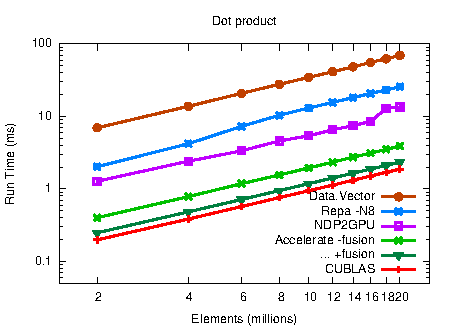
\includegraphics[width=0.8\textwidth]{images/sec-6/dotp/dotp}
    \end{center}
    \caption[Vector dot product kernel benchmarks]{Kernel runtimes for vector
        dot product, in Accelerate with and without optimisations, compared to
        other parallel GPU and CPU implementations. Note the log-log scale.}
    \label{fig:dotp}
\end{figure}

Without optimisations the Accelerate version executes in approximately twice the
time of the CUBLAS version. Since the individual aggregate operations consist of
only a single arithmetic operation each, the problem can not be a lack of
sharing.


\subsection{Too many kernels}

The slow-down in the unoptimised version is due to Accelerate generating one GPU
kernel function for each aggregate operation in the source program. The use of
two separate kernels requires the intermediate array produced by @zipWith@ to be
constructed in GPU memory before being immediately read back by @fold@. In
contrast, the CUBLAS version uses only a single kernel. As this is a simple
memory bound benchmark, we would expect the lack of fusion to double the
runtime, which is what we observe.

The fused version of dot product combines the aggregate computations by
embedding a function of type @(sh -> a)@ into the reduction, represented
here as the second argument to the constructor @Delayed@. This scalar
function does the work of element wise multiplying the two input vectors, and is
performed on-the-fly as part of the reduction kernel instead of requiring an
intermediate array. See Section~\ref{sec:array_fusion} for more information.
Applied to two manifest arrays, the following embedded program will be executed:

\begin{lstlisting}[style=haskell]
let a0 = use (Array ...) in
let a1 = use (Array ...) in
fold (\x0 x1 -> x0 + x1) 0.0
     (Delayed (intersect (shape a0) (shape a1))   -- extent of the input array
              (\x0 -> (a0!x0) * (a1!x0)))         -- function to generate a value at each index
\end{lstlisting}

While the fused Accelerate version is $30\times$ faster than the sequential
version executed on the CPU, it is still approximately $20\%$ slower than the
\marginnote{tk:check this}
hand-written CUBLAS version. As dot product is a computationally simple task,
any additional overheads in the implementation will be significant. To see why
this version is still slightly slower, we continue by analysing the generated
code to inspect it for sources of overhead.


% \subsection{Duplicate loop counters}
%
% The fused dot product operation will only perform the element wise
% multiplication of the two input arrays in the first step of the tree reduction
% (\S\ref{sec:parallel_reduction}). This occurs in the phase of the cascaded
% algorithm when individual threads sequentially sum multiple elements. After
% embedding the fused producer, the following CUDA code is generated for the inner
% loop of this step:
% %
% % pookie is the bestest
% % bubbaboo ish silly
% % kekekee
% % i can't put smiley faces in cause weird things happen
% % hehe^{this is my thesis
% % please like it
% % i worked really hard
% % and writed a lots
% % }<++>
% %
% %
% \begin{lstlisting}[style=cuda
%     ,firstnumber=18
%     ,label=lst:dotp_cuda
%     ,caption={Generated CUDA code for the first step of fused dot product}]
% for (ix += gridSize; ix < shapeSize; ix += gridSize) {
%     const Int64 v2 = ix;
%     const int v3 = toIndex(shIn0, shape(v2));
%     const int v4 = toIndex(shIn1, shape(v2));
%
%     x0 = arrIn0_a0[v3] * arrIn1_a0[v4];
%     y0 = x0 + y0;
% }
% \end{lstlisting}
% %
% We have four loop counters: @ix@, @v2@, @v3@ and @v4@ ---
% two for the source arrays and two to convert between the multidimensional and
% linear representations. These counters contain the same value and are
% incremented in lockstep. In addition to the superfluous arithmetic, the
% duplication of counters unnecessarily increases register pressure.
%
% \marginnote{this was unexpected}
% The corresponding section of PTX~\cite{NVIDIA:2012vj} code is for this loop is
% shown in Listing~\ref{lst:dotp_ptx}. To retrieve the data from the first input
% array, the input array pointer is retrieved (line~\ref{lst:dotp_ptx_ldparam}),
% the offset stored in register @rd16@ added to it
% (line~\ref{lst:dotp_ptx_add}), and then the value read from global memory at
% this address (line~\ref{lst:dotp_ptx_ldglobal}). Happily, we note that
% retrieving the second input element \emph{also} uses the offset stored in
% register @rd16@ (line~\ref{lst:dotp_ptx_ldglobal2}).
% %
%
% \begin{lstlisting}[style=ptx
%     ,float
%     ,firstnumber=103
%     ,label=lst:dotp_ptx
%     ,caption={[PTX code for the first step of fused dot product]
%         PTX code for the first step of fused dot product (sm13)}]
%  //  18          for (ix += gridSize; ix < shapeSize; ix += gridSize) {
%         cvt.u32.u16     %r10, %nctaid.x;
%         mul.lo.u32      %r11, %r10, %r1;
%         add.s32         %r12, %r11, %r7;
%         mov.s32         %r13, %r12;
%         setp.le.s32     %p2, %r8, %r12;
%         `%p2 bra        $Lt_0_13058;
%         cvt.s64.s32     %rd12, %r12;
%         cvt.s64.u32     %rd13, %r11;
% $Lt_0_14082:
%  //<loop> Loop body line 18, nesting depth: 1, estimated iterations: unknown
%         .loc    16      24      0
%  //  20              const int v3 = toIndex(shIn0, shape(v2));
%  //  21              const int v4 = toIndex(shIn1, shape(v2));
%  //  22
%  //  23              x0 = arrIn0\_a0[v3] * arrIn1\_a0[v4];
%  //  24              y0 = x0 + y0;
%         cvt.s32.s64     %rd14, %rd12;                           (@* \label{lst:dotp_ptx_cvt1} *@)
%         cvt.s32.s64     %r14, %rd14;
%         cvt.s64.s32     %rd15, %r14;                            (@* \label{lst:dotp_ptx_cvt3} *@)
%         mul.wide.s32    %rd16, %r14, 4;
%         .loc    16      17      0
%         ld.param.u64    %rd9, [__cudaparm_foldAll_arrIn0_a0];   (@* \label{lst:dotp_ptx_ldparam} *@)
%         .loc    16      24      0
%         add.u64         %rd17, %rd16, %rd9;                     (@* \label{lst:dotp_ptx_add} *@)
%         ld.global.f32   %f4, [%rd17+0];                         (@* \label{lst:dotp_ptx_ldglobal} *@)
%         .loc    16      17      0
%         ld.param.u64    %rd8, [__cudaparm_foldAll_arrIn1_a0];
%         .loc    16      24      0
%         add.u64         %rd18, %rd16, %rd8;
%         ld.global.f32   %f5, [%rd18+0];                         (@* \label{lst:dotp_ptx_ldglobal2} *@)
%         mad.f32         %f3, %f4, %f5, %f3;
%         add.s32         %r13, %r13, %r11;
%         add.s64         %rd12, %rd12, %rd13;
%         setp.gt.s32     %p3, %r8, %r13;
%         `%p3 bra        $Lt_0_14082;
%         bra.uni         $Lt_0_13058;
% $Lt_0_13314:
%         mov.f32         %f3, %f6;
% $Lt_0_13058:
%         .loc    16      27      0
%  //  25          }
% \end{lstlisting}
%
% In this case the CUDA compiler was able to coalesce our four counters into a
% single counter. This is because our definition of @toIndex@ specialised for
% one-dimensional indices @DIM1@ does \emph{not} do bounds checking:
% %
% \begin{lstlisting}[style=cuda]
% template <>
% static __inline__ __device__ Ix toIndex(const DIM1 sh, const DIM1 ix)
% {
%     return ix;
% }
% \end{lstlisting}
% %
% Since we do not check that the current index @ix@ is within bounds of the
% array shape @sh@, the compiler can see that the definitions of @v3@
% and @v4@ in Listing~\ref{lst:dotp_cuda} are identical. Similarly
% one-dimensional indices are just integers, and so the one-dimensional instance
% of @shape@ is the identity function. For higher dimensional shapes,
% however, this is not the case and @toIndex@ and @shape@ do real work
% to their arguments. As the shape @shIn0@ and @shIn1@ are inputs
% arguments to the kernel, the compiler will not be able to determine they are
% equivalent and so the counters would not be combined.
%
% Why don't we perform bounds checks in @toIndex@? Implementing exceptions in
% a massively parallel architecture is difficult, and support for throwing
% exceptions from kernel functions was only recently added for devices of compute
% capability 2.0 and later~\cite{NVIDIA:2012wf}. % [\SB.15]


\subsection{64-bit Arithmetic}

The host architecture that the Haskell program executes on is likely to be a
64-bit processor. If this is the case, then manipulating machine word sized
types such as @Int@ in embedded code must generate instructions to manipulate
64-bit integers in the GPU\@. On the other hand, CUDA devices are at their core
32-bit processors, and are thus optimised for 32-bit arithmetic. For example, our
Tesla GPU with compute capability 1.3 has a throughput of eight 32-bit
floating-point add, multiply, or multiply-add operations per clock cycle per
multiprocessor, but only a single operation per cycle per multiprocessor of the
64-bit equivalents of these~\cite{NVIDIA:2012wf}. % [\S5.4.1]
Additionally, while not explicitly stated, it appears that 64-bit integer
instructions are not natively supported on any architectures, and require
multiple clock cycles per instruction per multiprocessor.

The delayed producer function that is embedded into the consumer @fold@ kernel
corresponds to the operation @zipWith (*)@, and has concrete type
@(Exp (Z:.Int) -> Exp Float)@. Since this is executed on a 64-bit host machine,
the indexing operations must generate embedded code for 64-bit integers. See
Section~\ref{sec:instantiating_skeletons} for more information on code
generation, which produces the following CUDA code:
%
\begin{lstlisting}[style=haskell]
const Int64 v1 = ({ assert(ix >= 0 && ix < min(shIn1_0, shIn0_0)); ix; });
y0 = arrIn1_0[v1] * arrIn0_0[v1];
\end{lstlisting}
%
This is translated by the CUDA compiler into the following PTX assembly
code~\cite{NVIDIA:2012vj}, which is the lowest level representation accessible
to the developer:
%
\begin{lstlisting}[style=ptx]
//  13      const Int64 v1 = ({ assert(ix >= 0 && ix < min(shIn1_0, shIn0_0)); ix; });
        cvt.s64.s32     %rd5, %r5;
        mov.s64         %rd6, %rd5;
//  14
//  15      y0 = arrIn1_0[v1] * arrIn0_0[v1];
        mov.s64         %rd7, %rd6;
        mul.lo.u64      %rd8, %rd7, 4;
        ld.param.u64    %rd9, [__cudaparm_foldAll_arrIn1_0];
        ld.param.u64    %rd10, [__cudaparm_foldAll_arrIn0_0];
        add.u64         %rd11, %rd8, %rd9;
        ld.global.f32   %f1, [%rd11+0];
        add.u64         %rd12, %rd8, %rd10;
        ld.global.f32   %f2, [%rd12+0];
        mul.f32         %f3, %f1, %f2;
\end{lstlisting}
%
The first instruction converts the loop variable @ix@ --- which was not shown
but is declared with the C @int@ type --- to a 64-bit integer using the
@cvt.s64.s32@ instruction. The @assert@ function does not contribute anything in
this case as the kernel was not compiled with debugging enabled. Instructions in
PTX assembly are appended with the type of their operands, where @s64@ and @u64@
represent signed and unsigned 64-bit integers respectively, so it is clear that
the instructions in this fragment are manipulating 64-bit values.

In this instance, 64-bit arithmetic was introduced through the use of a
one-dimensional shape index, which has Haskell type @(Z :. Int)@ and corresponds
to a 64-bit wide integer on our host machine. Adding support for non-@Int@ shape
dimensions is left for future work.


\subsection{Non-neutral starting elements}
\label{sec:non-neutral_starting_elements}

In order to support efficient parallel execution, the @fold@ function in
Accelerate requires the combination function to be an associative operator.
However, we do not require the starting value to be a neutral element of the
combination function. For example, @fold (+) 42@ is valid in Accelerate, even
though @42@ is not the neutral element of addition.

While convenient for the user, this feature complicates the implementation. In
particular, threads can not initialise their local sum with the neutral element
during the first sequential reduction phase, and during the second cooperative
reduction step must be sure to only include elements from threads that were
properly initialised from the input array. See
Section~\ref{sec:parallel_reduction} for more information on the implementation
of parallel reductions in CUDA\@. Both of these restrictions necessitate
additional bounds checks, which increases overhead from ancillary instructions
that are not loads, stores, or arithmetic for the core computation. As the
summation reduction has low arithmetic intensity, which is the limiting factor
in the performance of this kernel~\cite{Harris:2007te}, additional bounds checks
further reduce performance.

It is left for future work to have operations such as @fold@ and @scan@ observe
when the combination function and starting element form a monoid, and provide
optimised kernels that avoid these extra administrative instructions. This is
the approach taken by, for example, Thrust~\cite{ThrustAParallelT:ub}.


\subsection{Kernel specialisation}

To further reduce instruction overhead, it is possible to completely unroll the
reduction by specialising the kernel for a specific block size. In CUDA this can
be achieved through the use of C++ templates. Branches referring to the template
parameter will be evaluated at compile time, resulting in a very efficient inner
loop.
%
\begin{lstlisting}[style=cuda]
template <unsigned int blockSize> __global__ void reduce(...) {
    ...
    if (blockSize > 512) {
    }
    if (blockSize > 256) {
    }
    ...
\end{lstlisting}

This technique has shown to produce significant gains in
practice~\cite{Harris:2007te}, although requires compiling a separate kernel for
each thread block size we wish to specialise for. Accelerate can achieve this
kind of kernel specialisation because the CUDA code is generated at program
runtime. However, since compilation also occurs at program runtime, this adds
significant additional runtime overhead. Since compiled kernels are cached and
reused, if we know that the reduction will be computed many times, the extra
compilation overhead can be amortized by the improved kernel performance, and
thus may be worthwhile. See Section~\ref{sec:dynamic_compilation} for more
information on the mechanism of compilation and code memoisation. Implementing
kernel specialisations, and evaluating their effectiveness, is left to future
work.


\section{Black-Scholes option pricing}
\label{sec:blackscholes}

The Black-Scholes algorithm is a partial differential equation for modelling the
evolution of a European-style stock option price under certain assumptions. The
corresponding Accelerate program is shown in Listing~\ref{lst:blackscholes}.
Given a vector of triples of the underlying stock price, strike price, and time
to maturity in years, the Black-Scholes formula computes the price of a call and
put option. The function @callput@ evaluates the Black-Scholes formula for
a single triple, and @blackscholes@ maps it over a vector of triples such
that all individual applications of the formula are executed in parallel.

\begin{lstlisting}[style=haskell_float
    ,float
    ,label=lst:blackscholes
    ,caption={Black-Scholes option pricing}]
horner :: Num a => [a] -> a -> a
horner coeff x =
  let madd a b  = a + x*b
  in
  x * foldr1 madd coeff

cnd' :: Floating a => a -> a
cnd' d =
  let poly      = horner coeff
      coeff     = [0.31938153, -0.356563782, 1.781477937, -1.821255978, 1.330274429]
      rsqrt2pi  = 0.39894228040143267793994605993438
      k         = 1.0 / (1.0 + 0.2316419 * abs d)
  in
  rsqrt2pi * exp (-0.5*d*d) * poly k

blackscholes :: Acc (Vector (Float, Float, Float)) -> Acc (Vector (Float, Float))
blackscholes = A.map callput
  where
  callput x =
    let (price, strike, years) = A.unlift x
        r       = A.constant riskfree
        v       = A.constant volatility
        v_sqrtT = v * sqrt years
        d1      = (log (price / strike) + (r + 0.5 * v * v) * years) / v_sqrtT
        d2      = d1 - v_sqrtT
        cnd d   = let c = cnd' d in d >* 0 ? (1.0 - c, c)
        cndD1   = cnd d1
        cndD2   = cnd d2
        x_expRT = strike * exp (-r * years)
    in
    A.lift ( price * cndD1 - x_expRT * cndD2                    -- call price
           , x_expRT * (1.0 - cndD2) - price * (1.0 - cndD1))   -- put price
\end{lstlisting}

Figure~\ref{fig:blackscholes} shows the result of running this code compared to
the implementation that ships with the CUDA SDK. Without optimisations, the
Accelerate version is almost twenty times slower than the equivalent
implementation in CUDA\@. As @blackscholes@ includes only one collective array
operation, the problem can not be a lack of fusion.

\begin{figure}
    \begin{center}
        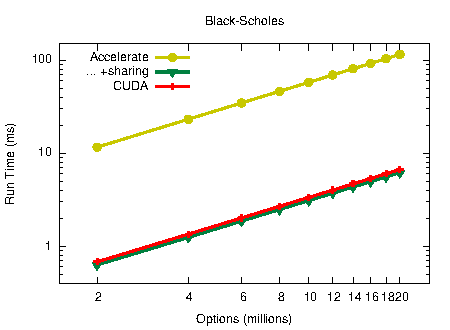
\includegraphics[width=0.8\textwidth]{images/sec-6/black-scholes/black-scholes}
    \end{center}
    \caption[Black-Scholes kernel benchmarks]{Kernel runtimes for Black-Scholes
        options pricing, in Accelerate with and without optimisations, compared
        to a hand-written CUDA version. Note the log-log scale.}
    \label{fig:blackscholes}
\end{figure}

\subsection{Too little sharing}

The function @callput@ from Listing~\ref{lst:blackscholes} includes a
significant amount of sharing: the helper functions @cnd'@ and hence
@horner@ are used twice --- for @d1@ and @d2@ --- and its
argument @d@ is used multiple times in the body. Furthermore, the
conditional expression @d >* 0 ? (1 - c, c)@ results in a branch that,
without sharing, results in a growing number of predicated instructions that
leads to a large penalty on the SIMD architecture of the GPU\@.

Without sharing the generated code requires 5156 instructions to calculate 128
options (2 thread blocks of 64 threads each) and results in significant warp
divergence which serialises portions of the execution. With sharing recovery the
generated code requires 628 instructions (one thread block of 128 threads) and
is actually slightly faster than the reference CUDA version because the latter
contains a common subexpression that was not spotted by the programmer and not
eliminated by the CUDA compiler. The common subexpression performs a single
multiplication. The CUDA version executes 652 instructions (128 threads per
block).


\section{Mandelbrot fractal}
\label{sec:mandelbrot}

The Mandelbrot set is generated by sampling values $c$ in the complex plane and
determining whether under iteration of the complex quadratic polynomial:
\[
z_{n+1} = z_{n}^{2} + c
\]
that the magnitude of $z$ (written $\left| z_{n} \right|$) remains bounded
however large $n$ gets. Images of the Mandelbrot set are created such that each
pixel corresponds to a point $c$ in the complex plane, and its colour depends on
the number of iterations $n$ before the relation diverges, where $z_{0} = c$.
The set of points forming the boundary of this relation forms the distinctive
and easily recognisable fractal shape shown in Figure~\ref{fig:mandelbrot}.

\begin{figure}
    \begin{center}
        \includegraphics[width=0.8\textwidth]{images/sec-6/mandelbrot/mandelbrot}
    \end{center}
    \caption[The Mandelbrot fractal]{Image of a Mandelbrot set with a
        continuously coloured environment. Each pixel corresponds to a point $c$
        in the complex plane, and its colour depends the number of iterations
        $n$ before the relation diverges. Centre coordinate
        $\left( -0.5+0i \right)$, horizontal width 3.2.}
    \label{fig:mandelbrot}
\end{figure}

\begin{table}
\centering
\small
\begin{tabu}{lrrrr}
\toprule

                        & \multicolumn{1}{c}{\textbf{Time}}
                        & \multicolumn{1}{c}{\textbf{Bandwidth}}
                        & \multicolumn{1}{c}{\textbf{Step}}
                        & \multicolumn{1}{c}{\textbf{Cumulative}} \\

\textbf{Benchmark}      & \multicolumn{1}{c}{\textbf{(ms)}}
                        & \multicolumn{1}{c}{\textbf{(GB/s)}}
                        & \multicolumn{1}{c}{\textbf{Speedup}}
                        & \multicolumn{1}{c}{\textbf{Speedup}} \\\midrule

Accelerate              &
                        &
                        &
                        & \\

Accelerate (+sharing)   &
                        &
                        &
                        & \\

Accelerate (+fusion)    &
                        &
                        &
                        & \\

Accelerate (+loop recovery)
                        &
                        &
                        &
                        & \\

Accelerate (+iteration)
                        &
                        &
                        &
                        & \\

CUDA (limit)            & 14.0
                        & 0.55
                        &
                        & \\

CUDA (avg)              & 5.0
                        & 1.53
                        & 2.79$\times$
                        & 2.79$\times$ \\

CPU (avg)               & 1389
                        & 0.006
                        &
                        & \\

\bottomrule
\end{tabu}
\caption[Mandelbrot fractal kernel benchmarks]{Mandelbrot fractal benchmarks in
    Accelerate with and without optimisations, compared to a hand written CUDA
    version. The benchmark computes the Mandelbrot set shown in
    Figure~\ref{fig:mandelbrot}, which has centre coordinates $-0.7 + 0i$ and
    width $3.067$. The CUDA (limit) benchmark computes every pixel to the
    maximum iteration count.}
\label{tab:mandelbrot}
\end{table}

Table~\ref{tab:mandelbrot} shows the results of the Mandelbrot program. As
expected, without fusion the performance of this benchmark is poor because
storing each step of the iteration saturates the memory bus, to the point that
reducing arithmetic intensity with sharing recovery provides no improvement.


\subsection{Fixed unrolling}

In order to meet the restrictions of what can be efficiently executed on
specialised hardware such as GPUs, Accelerate did not directly support any form
of iteration or recursion. To implement the recurrence relation we instead
define each step of computing $z_{n+1}$ given $z_n$ and $c$ as a collective
operation, and apply the operation a fixed number of times. The trick then is to
keep a pair @(z, i)@ for every point on the complex plane, where @i@ is the
iteration at which the point @z@ diverged. The code implementing this is shown
in Listing~\ref{lst:mandelbrot}.

\begin{lstlisting}[style=haskell_float
    ,label=lst:mandelbrot
    ,caption={Mandelbrot set generator, using fixed unrolling}]
mandelbrot
    :: forall a. (Elt a, IsFloating a)
    => Int
    -> Int
    -> Int
    -> Acc (Scalar (View a))
    -> Acc (Array DIM2 Int32)
mandelbrot screenX screenY depth view
  = P.snd . A.unzip
  $ P.foldr ($) zs0                                                                    -- (1)
  $ P.take depth (repeat step)
  where
    -- The view plane
    (xmin,ymin,xmax,ymax)     = unlift (the view)
    sizex                     = xmax - xmin
    sizey                     = ymax - ymin
    viewx                     = constant (P.fromIntegral screenX)
    viewy                     = constant (P.fromIntegral screenY)

    step :: Acc (Array DIM2 (Complex a, Int32))
         -> Acc (Array DIM2 (Complex a, Int32))
    step = A.zipWith iter cs

    iter :: Exp (Complex a) -> Exp (Complex a, Int32) -> Exp (Complex a, Int32)        -- (2)
    iter c zi = next (A.fst zi) (A.snd zi)
     where
      next :: Exp (Complex a) -> Exp Int32 -> Exp (Complex a, Int32)
      next z i =
        let z' = c + z*z
        in (dot z' >* 4) ? ( zi , lift (z', i+1) )                                     -- (3)

    dot :: Exp (Complex a) -> Exp a
    dot c = let r :+ i = unlift c
            in  r*r + i*i

    -- initial conditions for a given pixel in the window, translated to the
    -- corresponding point in the complex plane
    cs  = A.generate (constant $ Z :. screenY :. screenX) initial
    zs0 = A.map (\c -> lift (c, constant 0)) cs

    initial :: Exp DIM2 -> Exp (Complex a)
    initial ix = lift ( (xmin + (x * sizex) / viewx) :+ (ymin + (y * sizey) / viewy) )
      where
        pr = unindex2 ix
        x  = A.fromIntegral (A.snd pr :: Exp Int)
        y  = A.fromIntegral (A.fst pr :: Exp Int)
\end{lstlisting}

\begin{enumerate}
\item The function @step@ advances the entire complex plane by one iteration of
    the recurrence relation. This function is repeated @depth@ number of times,
    and the sequence combined by folding together with function application
    @($)@. This effectively unrolls the loop to @depth@ iterations.

\item The function @iter@ computes the next value in the sequence for a single
    point on the complex plane. If the point has diverged, we return the
    iteration count at which divergence occurred, otherwise the new value @z'@
    is returned and the iteration count @i@ is increased.

\item The conditional test is performed by the @(?)@ operator. Recall that GPUs are
    designed to do the same thing to lots of different data at the same time,
    whereas we want to do something different depending on whether or not a
    particular point has diverged. While we can not avoid having some kind of
    conditional in the code, we ensure there is only a bounded amount of
    divergence by having just one conditional per iteration, and a fixed number
    of iterations.

\end{enumerate}

Array fusion applied to the program in Listing~\ref{lst:mandelbrot} results in
the @depth@ copies of the function @step@ being combined into a single kernel.
As seen in Table~\ref{tab:mandelbrot}, while fusion improves the performance of
this program, it is still slower than the hand written version.

This slowdown is because the fused code generates a completely unrolled loop,
with @depth@ copies of the function body. Unrolling loops not only increases
instruction counts, but can often increase register lifetimes because of the
scheduling of loads and stores. In particular, stores are pushed down and loads
moved up in the instruction stream, which results in temporary scalar lifetimes
being longer. The unrolled code requires TK registers, resulting in a
multiprocessor occupancy of TK\%. Since the Mandelbrot program is limited by
computation, reducing the number of resident threads has a corresponding
reduction on maximum performance.

% \begin{lstlisting}[style=cuda
%     ,firstnumber=24]
% const float v13 = v10 * v10 - v11 * v11;                // single application of \texttt{step}
% const float v14 = v10 * v11 + v11 * v10;
% const float v15 = v8 + v13;
% const float v16 = v9 + v14;
% const Word8 v17 = v15 * v15 + v16 * v16 > 4.0f;
% const float v18 = v17 ? v10 : v15;
% const float v19 = v17 ? v11 : v16;
% const Int64 v20 = v17 ? v12 : (Int64) 1;
%   // repeats 255 times\ldots
% \end{lstlisting}


\subsection{Loop recovery}

Loop unrolling or loop unwinding is a loop transformation technique that
attempts to optimise a program's execution speed by reducing or eliminating
instructions that control the loop, such as branching and the end-of-loop test.
Loop unrolling does not always improve performance, however, because it may lead
to, for example, increased register usage.

Applying the fusion transformation to the Mandelbrot program shown in
Listing~\ref{lst:mandelbrot} resulted in a single kernel with @depth@ copies of
the function @iter@. In essence, the loop computing the Mandelbrot recurrence
relation has been completely unrolled. Unfortunately, the fused program does not
match the performance of the hand written version, because (a)
The program has a increased register usage; and (b) the conditional test is
still performed at the end of each copy of the loop body, so there is no
reduction in the overall number of instructions and branches executed.

We attempted to reduce these overheads by re-introducing explicit scalar loops
into the generated code. Recovering scalar loops then enables a backend to
generate explicit @for@ loops in the target language, and the compiler then
makes the decision of whether or not to unroll the loop. The following pair of
rewrite rules are used.
%
\begin{lstlisting}[style=Haskell,numbers=none,mathescape]
%\bf$\langle$ loop introduction $\rangle$%
    let x =
        let y = e1
        in e2
    in e3
    $\mapsto$
    iterate[2] (\y -> e2) e1            %\rm if \texttt{e2} $\equiv$ \texttt{e3}%

%\bf$\langle$ loop joining $\rangle$%
    let x = iterate[n] (\y -> e2) e1
    in e3
    $\mapsto$
    iterate[n+1] (\y -> e2) e1          %\rm if \texttt{e2} $\equiv$ \texttt{e3}%
\end{lstlisting}

As seen in Table~\ref{tab:mandelbrot}, loop recovery shows a good increase in
performance compared to the fused and unrolled result, but is slower than the
hand written CUDA program because every thread always executes until the
iteration limit, even if it diverges immediately, and must maintain this extra
information of whether or not the thread has diverged yet.


\subsection{Explicit iteration}

Following our most recent published results~\cite{McDonell:2013wi}, we added
explicit value recursion constructs to the source and target languages. Robert
Clifton-Everest implemented the necessary changes to the sharing recovery
algorithm, while I implemented the backend changes for code generation and
execution. The new function @while@ applies the given function, starting with
the initial value, as long as the test function continues to evaluate to @True@.
%
\begin{lstlisting}[style=haskell]
while :: Elt e
      => (Exp e -> Exp Bool)            -- conditional test
      -> (Exp e -> Exp e)               -- function to iterate
      -> Exp e                          -- initial value
      -> Exp e
\end{lstlisting}
%
The Mandelbrot program using explicit iteration is shown in
Listing~\ref{lst:mandelbrot_loop}, where the common parts to the @where@ clause
in Listing~\ref{lst:mandelbrot} have been elided. Note that in contrast to the
implementation based on fixed unrolling, the function will stop executing as
soon as the relation diverges, rather than always continuing to the iteration
limit even if the point has already diverged.

\begin{lstlisting}[style=haskell_float
    ,label=lst:mandelbrot_loop
    ,caption={Mandelbrot set generator, using explict iteration}]
mandelbrot
    :: forall a. (Elt a, IsFloating a)
    => Int
    -> Int
    -> Int
    -> Acc (Scalar (View a))
    -> Acc (Array DIM2 Int32)
mandelbrot screenX screenY depth view =
  generate (constant (Z :. screenY :. screenX))
           (\ix -> let c = initial ix
                   in  A.snd $ A.while (\zi -> A.snd zi <* lIMIT &&* dot (A.fst zi) <* 4)
                                       (\zi -> lift1 (next c) zi)
                                       (lift (c, constant 0)))
  where
    lIMIT = P.fromIntegral depth

    next :: Exp (Complex a) -> (Exp (Complex a), Exp Int32) -> (Exp (Complex a), Exp Int32)
    next c (z, i) = (c + (z * z), i+1)
\end{lstlisting}

With respect to implementation on SIMD architectures such as CUDA, while both
the fixed unrolling and explicit iteration methods have a conditional test that
introduces thread divergence, it is important to note that the behaviour of the
divergence is different for each method. In the fixed unrolling case, both
branches of the conditional must be executed to keep track of whether the
element has already diverged. This results in threads following separate
execution paths, where threads that follow the @True@ branch execute while all
other threads sit idle, then execution switches to the @False@ branch and the
first set of threads sit idle. In contrast, in the explicit iteration case,
threads exit the loop as soon as their point on the complex plane diverges, and
then simply wait for all other threads in their SIMD group to complete their
calculation and catch up.

While the introduction of explicit value recursion required changes to the
source language program, as seen in Table~\ref{tab:mandelbrot}, performance
improves significantly. Additionally, if all threads in the SIMD group diverge
quickly, this can save a significant amount of redundant computation.
Table~\ref{tab:mandelbrot} also shows the difference in execution time between
computing the entire fractal shown in Figure~\ref{fig:mandelbrot}, where all
points diverge at different depths in the sequence (avg), compared to a region
where all threads continue to the iteration limit (limit).


\subsection{Unbalanced workload}

In order to manage the unbalanced workload, the hand-written CUDA version
includes a custom thread-block scheduler. Avoiding thread divergence in CUDA
programs is an active area of research~\cite{Zhang:2010jc}. TK.

% The final problem with the Mandelbrot program is due to the initial formulation
% of the program using a fixed unrolling, as we must handle application of the
% function to elements which have already diverged. As explained, this is to
% ensure that all threads [in a warp] continue doing the same thing, which avoids
% excessive SIMD divergence, but means that the computation always proceeds to the
% iteration limit.
%
% For the Mandelbrot program threads only diverge in the sense that they are
% either still computing the recurrence relation, or the point is not in the set
% and the computation has completed; threads do not diverge to follow separate
% execution paths. The latter type of SIMD divergence is what we really need to
% avoid, because this results in predicated execution: threads taking the
% @true@ path of a branch execute while all other threads sit idle, then
% execution switches to the @false@ branch while the first set of threads
% idle.
%
% The CUDA version is faster because threads exit the loop as soon as their point
% in the complex plane diverges. Although once a thread completes it sits idle
% until all threads in the group complete their calculation, if all the points
% within a group of threads diverge quickly this can save a significant amount of
% work. Table~\ref{tab:mandelbrot} shows the difference in execution time when
% displaying the entire fractal (avg), where points diverge at varying iteration
% depths in the sequence, compared to a region where all thread continue to the
% iteration limit (limit). In order to manage this unbalanced workload, the CUDA
% version additionally includes a custom thread block scheduler.
%
% This test demonstrates that while loop recovery offered a significant
% performance benefit for free, it would be beneficial to expose looping
% constructs in the source language as well, rather than relying on potentially
% fragile post-hoc transformations. Avoiding thread divergence in CUDA programs is
% an active area of research~\cite{Zhang:2010jc}.

\subsection{Passing inputs as arrays}

Note that in the definition of @mandelbrot@, the current view bounds are passed
as a scalar array. Why don't we pass these values as plain @Float@s? When the
program runs, Accelerate converts the program into a series of CUDA kernels,
each of which must be compiled and loaded onto the
GPU~(\S\ref{sec:code_generation}). Since compilation can take a while,
Accelerate remembers the kernels it has seen before and reuses
them~(\S\ref{sec:dynamic_compilation}). Our goal with @mandelbrot@ is to make a
kernel that will be reused, otherwise the overhead of compiling a new kernel
each time the view is changed will ruin performance.

By defining the @view@ as a scalar array, we ensure that it is defined
\emph{outside} the call to @generate@. If we don't do this, a different value
for the view parameter will be embedded directly into each call to the
@generate@ function, which will defeat Accelerate's caching of CUDA kernels.

Any scalar values that we wish to be treated as function parameters must be
lifted to array variables. This is because Accelerate currently does not support
nested data parallelism, so our internal representation of array terms is closed
with respect to scalar variables.
% to ensure that array computations can not depend on scalar values.
Adding support for nested data parallelism in Accelerate is an active area of
research. With it, it may be possible to avoid lifting free scalar variables to
the array level in order to correctly cache kernels.


\section{N-body gravitational simulation}
\label{sec:nbody}

\begin{figure}
    \begin{center}
        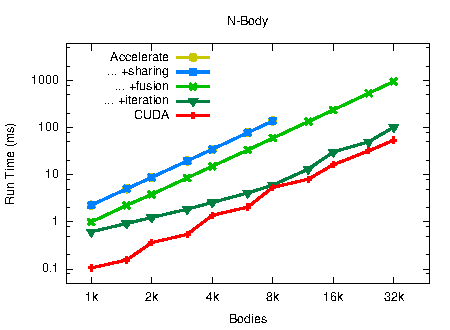
\includegraphics[width=0.8\textwidth]{images/sec-6/nbody/nbody}
    \end{center}
    \caption[N-body gravitational simulation kernel benchmarks]{Kernel runtimes
        for the $n$-body gravitational simulation, in Accelerate with and
        without optimisations, compared to a hand-written CUDA implementation.
        Note the log-log scale.}
    \label{fig:nbody}
\end{figure}

The $n$-body example simulates the Newtonian gravitational forces on a set of
massive bodies in 3D space, using the na\"ive $\mathcal{O}\left( n^{2} \right)$
algorithm. In a data-parallel setting, the natural way to express this algorithm
is first to compute the forces between every pair of bodies, before adding the
forces applied to each body using a segmented sum. Without fusion this approach
also requires $\mathcal{O}\left( n^{2} \right)$ space for the intermediate array
of forces, which exhausts the memory of our device (4GB!) when using more than
about five thousand bodies. With fusion, the reduction operation consumes each
force value on-the-fly, so that the program only needs $\mathcal{O}\left( n
\right)$ space to store the final force values. The core of the $n$-body
simulation is shown in Listing~\ref{lst:nbody}, where @accel@ calculates
the acceleration between two particles, and @(.+.)@ component-wise sums the
acceleration of a particle along each $x$, $y$ and $z$ axis.

\begin{lstlisting}[style=haskell_float
    ,label=lst:nbody
    ,caption={$N$-body gravitational simulation, using parallel reduction}]
calcAccels :: Exp Float -> Acc (Vector Body) -> Acc (Vector Accel)
calcAccels epsilon bodies
  = let n       = A.size bodies
        cols    = A.replicate (lift $ Z :. n :. All) bodies
        rows    = A.replicate (lift $ Z :. All :. n) bodies
    in
    A.fold (.+.) (vec 0) $ A.zipWith (accel epsilon) rows cols
\end{lstlisting}


\subsection{Sequential iteration}

Even with fusion, the reference CUDA version is over $10\times$ faster. Although
the fused program requires only $\mathcal{O}\left( n \right)$ space, it still
requires all $\mathcal{O}\left( n^2 \right)$ memory accesses, and $n^{2}$
threads to cooperatively compute the interactions.

With the addition of sequential iteration following our most recent
publication~\cite{McDonell:2013wi}, we can emit an alternative implementation.
Rather than computing all interactions between each pair of bodies and reducing
this array in parallel, we express the program as a parallel map of sequential
reductions, as shown in Listing~\ref{lst:nbody_seq}. Although the program still
performs all $n^{2}$ memory accesses, since all threads access the @bodies@
array in sequence, these values can be cached efficiently by the GPU, and the
actual bandwidth requirements to main memory are reduced.

\begin{lstlisting}[style=haskell_float
    ,label=lst:nbody_seq
    ,caption={$N$-body gravitational simulation, using sequential reduction}]
calcAccels :: Exp R -> Acc (Vector PointMass) -> Acc (Vector Accel)
calcAccels epsilon bodies
  = let move body = A.sfoldl (\acc next -> acc .+. accel epsilon body next)
                             (vec 0)
                             (constant Z)
                             bodies
    in
    A.map move bodies
\end{lstlisting}


\subsection{Use of Shared Memory}

In CUDA, the memory hierarchy of the device is made explicit to the programmer,
including a small on-chip shared memory region threads can use to share data,
that is essentially a software managed cache~\cite{NVIDIA:2012wf}.

The program shown in Listing~\ref{lst:nbody} uses the shared memory region to
share computations while computing the parallel reduction. The second
implementation shown in Listing~\ref{lst:nbody_seq} does not use shared memory
at all, but rather relies on hardware caching. Similar to our latter
implementation, the CUDA program is also implemented as a parallel map of
sequential reductions, but explicitly uses the shared memory region to share the
particle mass and position data between threads, rather than rely on hardware
caching. Since the shared memory region is very low latency, the CUDA program
remains faster. Automatic use of shared memory is a separate consideration to
the optimisations discussed in this work, and remains an open research
problem~\cite{Ma:2010ft}.

% This reduces the bandwidth requirement of the program by a factor of the number
% of threads in a block (256) but requires each thread to sum its particle
% interactions sequentially in $\mathcal{O}\left( n \right)$ time. The Accelerate
% version uses shared memory to perform a tree-reduction in $\mathcal{O}\left(
% \log n \right)$ time (\S\ref{sec:parallel_reduction}) but requires all $n^{2}$
% memory transfers. For this bandwidth bound application, making the trade-off of
% parallelism for bandwidth clearly wins. Automatic use of shared memory is a
% separate consideration to the optimisations discussed in this work, and remains
% an open research problem~\cite{Ma:2010ft}.


\section{Fluid Flow}
\label{sec:fluid}

The fluid flow example implements Jos Stam's stable fluid
algorithm~\cite{Stam:1999ey}, which is a fast approximate algorithm intended for
animation and games, rather than accurate engineering simulation. An example
sequence is shown in Figure~\ref{fig:fluid_steps}.

\begin{figure}
    \begin{center}
        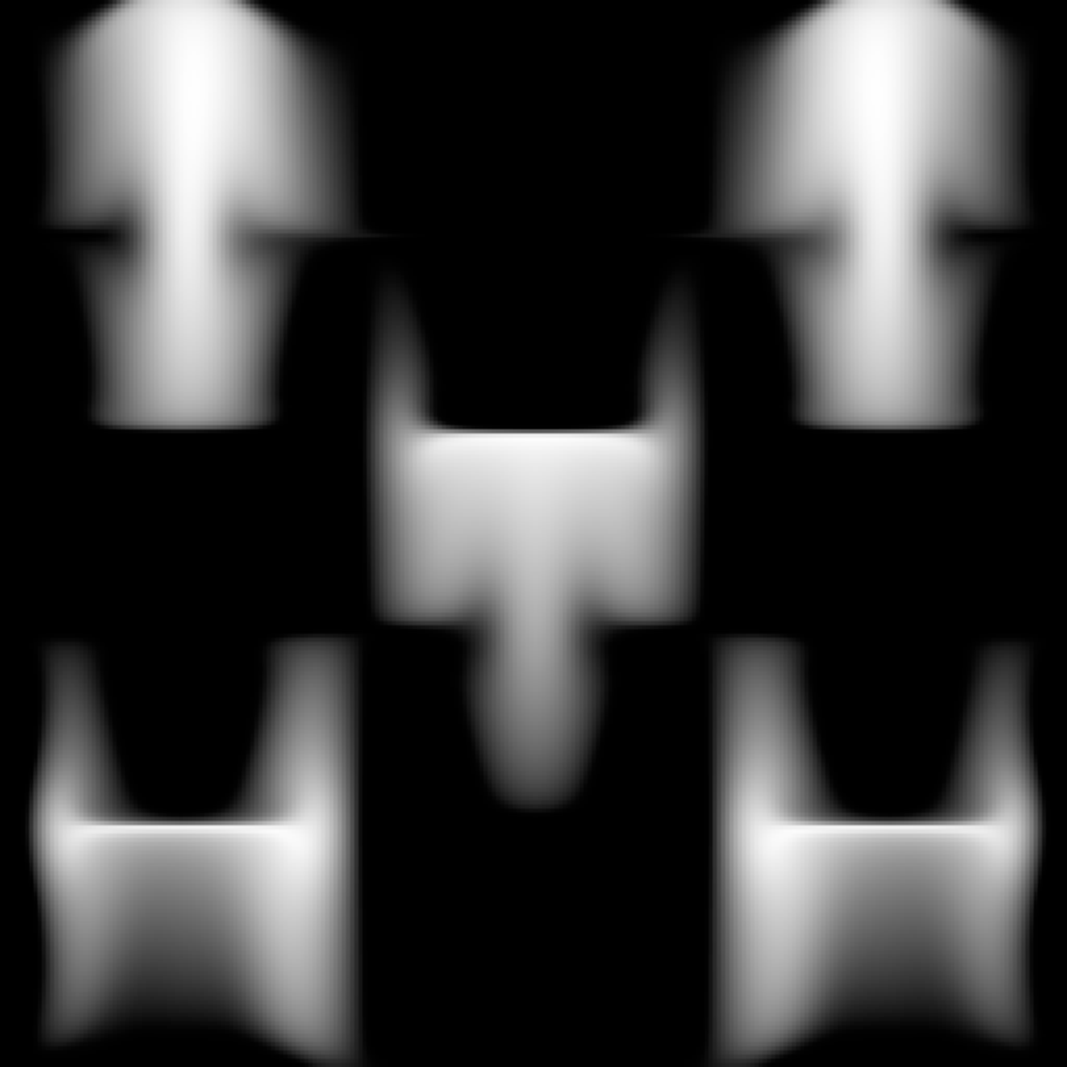
\includegraphics[width=0.3\textwidth]{images/sec-6/fluid/fluid-10}
        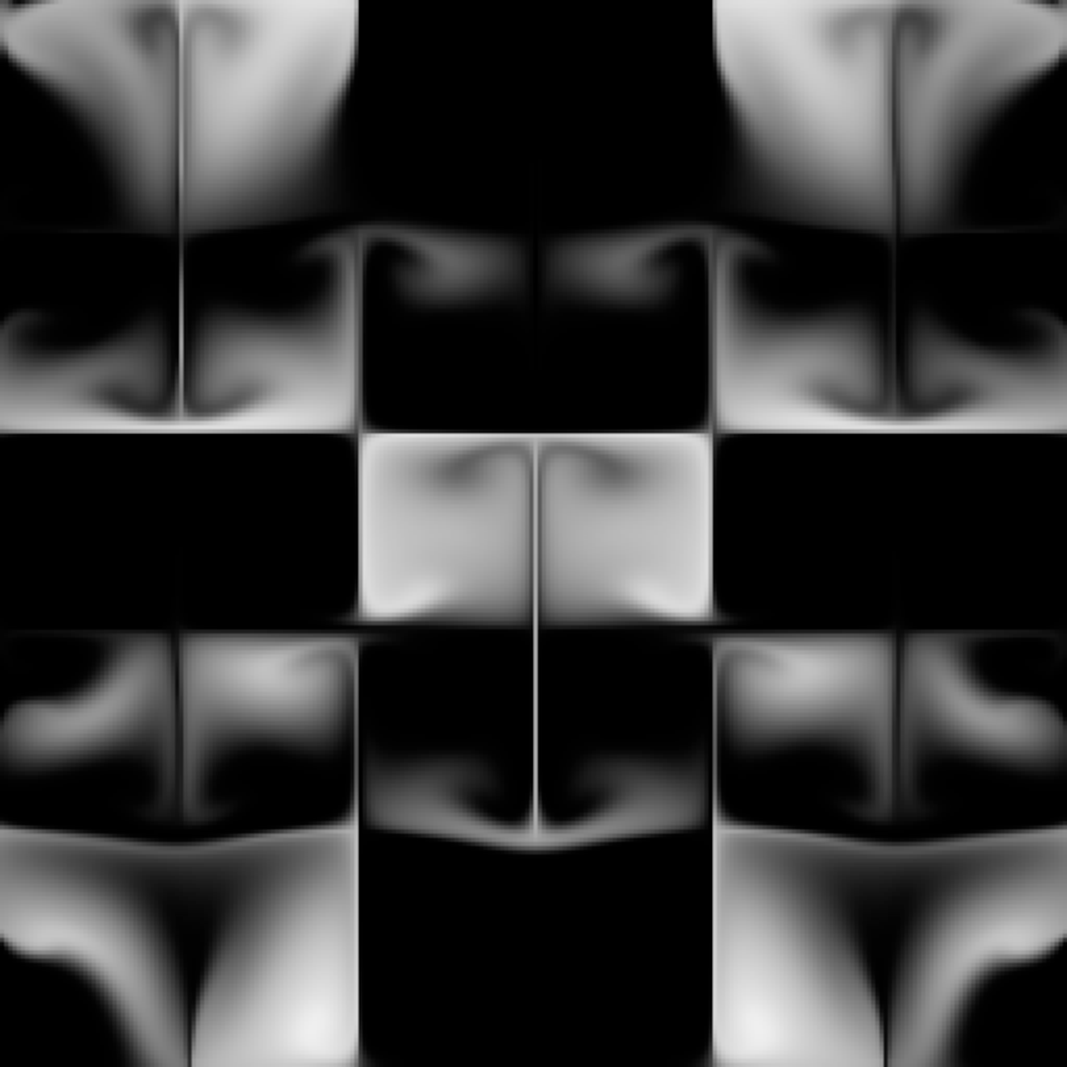
\includegraphics[width=0.3\textwidth]{images/sec-6/fluid/fluid-50}
        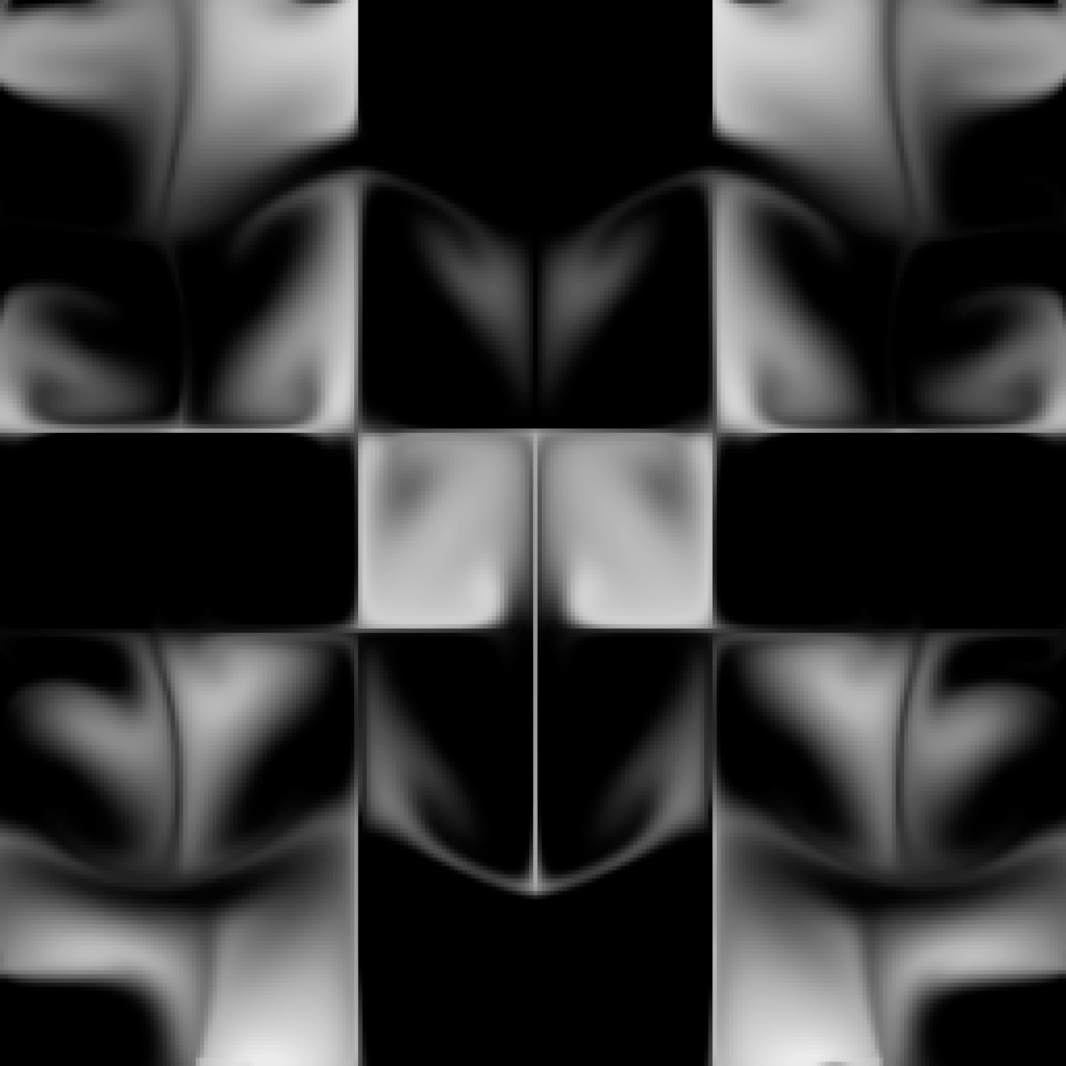
\includegraphics[width=0.3\textwidth]{images/sec-6/fluid/fluid-75}
    \end{center}
    \caption[Example of the fluid flow simulation]{An example showing the
        progression of the fluid flow simulation for a set of initial conditions
        after 10 (left), 50 (centre) and 75 (right) steps.}
    \label{fig:fluid_steps}
\end{figure}

The core of the algorithm is a finite time step simulation on a grid,
implemented as a matrix relaxation involving the discrete Laplace operator
($\nabla^2$). This step, known as the linear solver, is used to diffuse the
density and velocity fields throughout the grid, as well as apply a projection
operator to the velocity field to ensure it conserves mass. The linear solver is
implemented in terms of a stencil convolution, repeatedly computing the
following for each grid element to allow the solution to converge:
\[
u_{i,j}^{''} = \left( u_{i,j} + a \cdot \left( u'_{i-1,j}+u'_{i+1,j}+u'_{i,j-1}+u'_{i,j+1} \right) \right) / c
\]
Here, $u$ is the grid in the previous time step, $u'$ the grid in the current
time step and previous relaxation iteration, and $u''$ the current time step and
iteration. The values $a$ and $c$ are constants chosen by the simulation
parameters.

\begin{figure}
    \begin{center}
        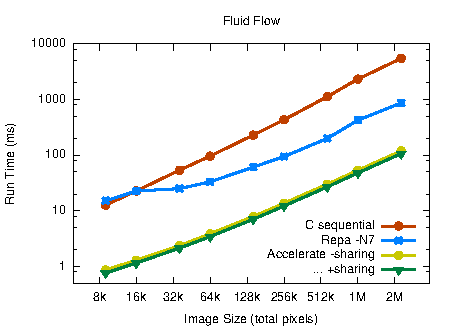
\includegraphics[width=0.8\textwidth]{images/sec-6/fluid/fluid}
    \end{center}
    \caption[Fluid flow simulation kernel benchmarks]{Kernel runtimes for the
        fluid flow simulation, in Accelerate with and without optimisations,
        compared to sequential and parallel CPU implementations. Running the
        Repa program with seven threads on the eight cores was found to be
        faster. Note the log-log scale.}
    \label{fig:fluid}
\end{figure}

Figure~\ref{fig:fluid} compares Accelerate to a parallel implementation written
in Repa and running on the host CPU \cite{Lippmeier:2012gx}. The program is
extremely memory intensive, performing approximately 160 convolutions of the
grid per time step. Given the nature of the computation, we find that the raw
bandwidth available on the CUDA device, which is much greater than that
available to the CPU, results in correspondingly shorter run times. Since the
program consists of a sequence of stencil operations, fusion does not apply to
this program. Sharing recovery has a surprisingly minimal impact because the
implementation of stencils always shares some parts of the computation: namely
access to the grid elements $u_{xy}$, precisely because these operations are so
expensive.

The CUDA SDK sample programs includes a version of Jos Stam's fluid flow
algorithm, but that is computed using Fourier transforms and is intermingled
with OpenGL code for the visualisation, so we can not directly compare to that
implementation.

% \note{tk: example showing performance of \code{map (+1)} versus the equivalent
% of using a stencil: extra addressing arithmetic should be significant. For fluid
% flow, the actual computation time (probably) greatly outweighs the extra
% arithmetic.}
%
% \note{TK: Check the fluid demo that is part of the CUDA SDK, it looks like it
% might implement something similar.}


\section{Canny edge detection}
\label{sec:canny}

The edge detection example applies the Canny algorithm~\cite{Canny:1986et} to
rectangular images of various sizes. Figure~\ref{fig:canny} compares Accelerate
to parallel implementations on the CPU and GPU\@. The overall algorithm consists
of seven distinct phases, the first six of which are naturally data parallel and
are performed on the GPU\@. The last phase uses a recursive algorithm to
``connect'' the pixels that make up the output lines. In our implementation this
phase is performed on the CPU, which requires the image data to be transferred
from the GPU back to the CPU for processing, and accounts for the non-linear
slowdown visible with smaller image sizes. In contrast, OpenCV is able to
perform the final step on the GPU\@. The benchmark ``Accelerate (whole
program)'' includes the time to transfer the image data back to the host for the
final processing step. Also shown are the run times for just the first six data
parallel phases, which exhibit linear speedup and do not include data transfer
to the host.

\begin{figure}
    \begin{center}
        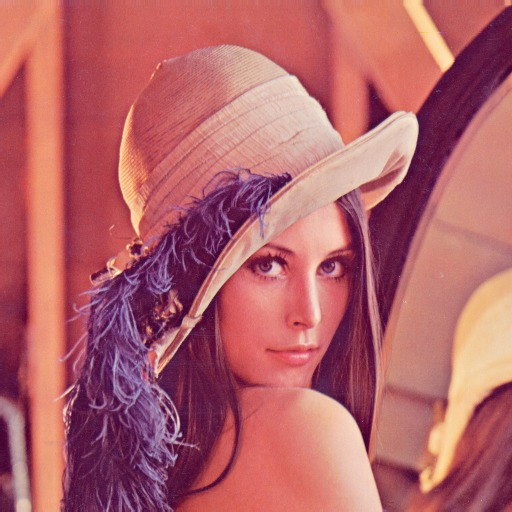
\includegraphics[width=0.45\textwidth]{images/sec-6/canny/lena}
        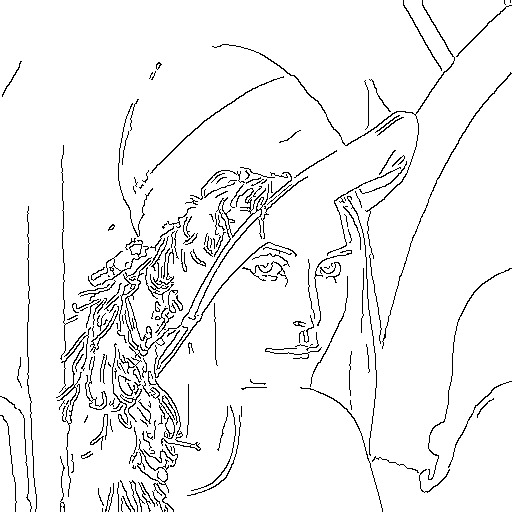
\includegraphics[width=0.45\textwidth]{images/sec-6/canny/lena-edges}
    \end{center}
    \caption[Example of the Canny edge detection algorithm]{An example of the
        Canny algorithm applied to the Lena standard test image (left) which
        identifies edge pixels in the image (right).}
    \label{fig:lena}
\end{figure}

Neglecting the final phase, note that the data parallel phase is still slightly
slower than in OpenCV. As discussed in
Section~\ref{sec:parallel_stencil}, this is because the stencil kernels
in Accelerate currently make a test for every array access to see if the element
is in bounds, or if it lies outside the array and needs to be handled specially,
even though the vast majority of points in the array are far from the boundary.

\begin{figure}
    \begin{center}
        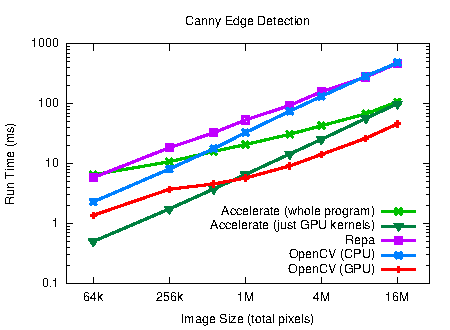
\includegraphics[width=0.8\textwidth]{images/sec-6/canny/canny}
    \end{center}
    \caption[Canny edge detection benchmarks]{Runtimes for the Canny edge
        detection algorithm, comparing the Accelerate kernels and whole program
        to sequential and parallel implementations. Note the log-log scale.}
    \label{fig:canny}
\end{figure}


\subsection{Stencil merging}

Two of the data parallel stages of the Canny algorithm are the calculation of
the image intensity gradients by convolving the image with the $3\times3$
kernels shown below. This convolution, known as the Sobel operator, is a
discrete differentiation operator that computes an approximation of the
horizontal and vertical image gradients.
%
\begin{equation*}
    \text{Sobel}_x =
        \begin{bmatrix*}[r]
          -1 & 0 & 1 \\
          -2 & 0 & 2 \\
          -1 & 0 & 1
        \end{bmatrix*}
    \qquad
    \text{Sobel}_y =
        \begin{bmatrix*}[r]
           1 &  2 &  1 \\
           0 &  0 &  0 \\
          -1 & -2 & -1
        \end{bmatrix*}
\end{equation*}

There is a significant amount of sharing between these two kernels, in terms of
the coefficients required to compute the derivative at each point. Thus, it
could be beneficial to merge these two stencils into a single kernel, rather
than computing them separately. As with all shortcut fusion methods, the system
presented here does not combine multiple passes over the same array into a
single traversal that computes multiple results. We leave this, as well as other
significant stencil
optimisations~\cite{Henretty:2013wb,Kamil:2006un,Lesniak:2010}, to future work.

% We leave this to future work,
% for example, in the style of data flow fusion~\cite{Lippmeier:2013vz}.


\section{Radix sort}

The radix sort benchmark implements a simple parallel radix sort algorithm as
described by \citet{Blelloch:1990vl} to sort an array by an integral key. We
compare our implementation of Blelloch's algorithm in Accelerate, shown in
Listing~\ref{lst:radixsort}, to one written in Nikola~\cite{Mainland:2010vj},
which is also an embedded language in Haskell for CUDA programming.%
\footnote{To be more specific, we estimate based on the results presented in the
paper~\cite{Mainland:2010vj} as Nikola no longer compiles with recent versions
of GHC, and the development version to replace it is not yet complete.
Nevertheless, results are informative as the same GPU, a Tesla T10, is used in
both cases.}
For this benchmark the Accelerate code is faster than Nikola, because Nikola is
limited to single kernel programs so must transfer every intermediate result
back to the host. Additionally, we are faster than a sequential radix sort
implementation using \texttt{Data.Vector} for as few as $\sim256$ elements,
whereas Nikola requires a dataset of about 32kB before the additional
parallelism of the GPU outperforms the sequential
version~\cite{Mainland:2010vj}.

\begin{lstlisting}[style=haskell_float
    ,label=lst:radixsort
    ,caption={Radix sort algorithm}]
class Elt e => Radix e where
  passes :: e -> Int                            -- number of passes (bits) required to sort this key type
  radix  :: Exp Int -> Exp e -> Exp Int         -- extract the $n^{th}$ bit of the key

sortBy :: forall a r. (Elt a, Radix r)
       => (Exp a -> Exp r)
       -> Acc (Vector a)
       -> Acc (Vector a)
sortBy rdx arr = foldr1 (>->) (P.map radixPass [0..p-1]) arr    -- loop over bits of the key, low\ldots
  where                                                         -- \ldots bit first to maintain sort order
    p           = passes (undefined :: r)
    deal f x    = let (a,b) = unlift x in (f ==* 0) ? (a,b)

    radixPass k v =
      let k'    = unit (constant k)                             -- to create reusable kernels
          flags = A.map (radix (the k') . rdx) v                -- extract the sort key
          idown = prescanl (+) 0 . A.map (xor 1)        $ flags -- move elements to the beginning\ldots
          iup   = A.map (size v - 1 -) . prescanr (+) 0 $ flags -- \ldots end of the vector
          index = A.zipWith deal flags (A.zip idown iup)
      in
      permute const v (\ix -> index1 (index!ix)) v              -- move elements to new position
\end{lstlisting}

The @radixPass@ function sorts the vector @v@ based on the value of
bit @k@; moving elements with a zero at that bit to the beginning of the
vector and those with a one bit to the end. This simple algorithm requires
$b$ iterations to sort an array of elements whose keys are $b$-bits wide, and
each pass requires multiple traversals of the array.

\begin{figure}
    \begin{center}
        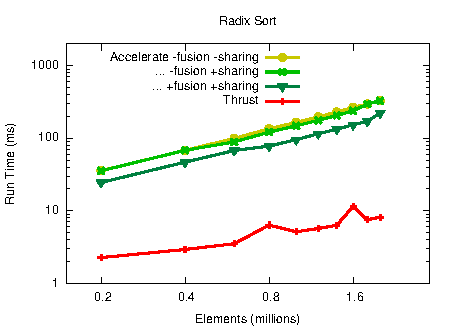
\includegraphics[width=0.8\textwidth]{images/sec-6/radixsort/radixsort}
    \end{center}
    \caption[Radix sort kernel benchmarks]{Kernel runtimes for the radix sort benchmark
        of signed 32-bit integers, comparing the Accelerate version to other
        parallel implementations. Note the log-log scale.}
    \label{fig:radixsort}
\end{figure}

As seen in Figure~\ref{fig:radixsort}, the absolute performance of this simple
algorithm, which sorts the array by a single bit at a time, is quite low.
Implementations of radix sort optimised for the CUDA
architecture~\cite{Satish:2009kx,Merrill:2011bz,ThrustAParallelT:ub}, are
approximately $10\times$ faster because they make efficient use of memory
bandwidth and on-chip shared memory to sort keys by 8-bits at a time. Such
implementations are, essentially, different algorithms than Blelloch's radix
sort algorithm that we have implemented here, but serve to illustrate the
absolute performance of the device. To address this we have implemented a
foreign function interface for Accelerate to take advantage of existing
high-performance libraries (\S\ref{sec:ffi}). The foreign function interface is
orthogonal to the work presented here of optimising programs written in the
Accelerate language. Useful future work would be to combine a fast-yet-fixed
foreign implementation with a more generic interface, using a method such
as~\cite{Henglein:2013dd}.


\section{Sparse-matrix vector multiplication}
\label{sec:smvm}

% \marginnote{tk: redo bechmarks}
\newcommand\spyplot[1]{\parbox[c][1.1cm][c]{1.1cm}{\includegraphics[width=1cm]{images/sec-6/smvm/#1}}}

\begin{table}
\centering
\small
\begin{tabu}{X[-1cm]X[2lm]cX[-1cb]rrr} \toprule

\textbf{spyplot}
& \textbf{Description}
& \textbf{Dimensions}
& \textbf{Nonzeros (nnz/row)}
& \multicolumn{1}{c}{\rotatebox{90}{\textbf{CUSP}}}
& \multicolumn{1}{c}{\rotatebox{90}{\textbf{Accelerate}}}
& \multicolumn{1}{c}{\begin{sideways}%
    \parbox{\widthof{\bf Accelerate}}%
    {\centering\textbf{Accelerate no fusion}}%
    \end{sideways}}
\\ \midrule

\spyplot{dense2} % Dense
& Dense matrix in sparse format
& 2K $\times$ 2K
& 4.0M (2K)
& 14.48 & 14.62 & 3.41
\\

\spyplot{pdb1HYS} % Protein
& Protein data bank 1HYS
& 36K $\times$ 36K
& 4.3M (119)
& 13.55 & 13.65 & 0.26
\\

\spyplot{consph} % FEM / Spheres
& FEM concentric spheres
& 83K $\times$ 83K
& 6M (72)
& 12.63 & 9.03 & 4.70
\\

\spyplot{cant} % FEM / Cantilever
& FEM cantilever
& 62K $\times$ 62K
& 4M (65)
& 11.98 & 7.96 & 4.41
\\

\spyplot{pwtk} % Wind Tunnel
& Pressurised wind tunnel
& 128K $\times$ 128K
& 11.6M (53)
& 11.98 & 7.33 & 4.62
\\

\spyplot{rma10} % FEM/Harbour
& 3D CFD of Charleston harbour
& 47K $\times$ 47K
& 2.37M (50)
& 9.42 & 6.14 & 0.13
\\

\spyplot{qcd5_4} % QCD
& Quark propagators (QCD/LGT)
& 49K $\times$ 49K
& 1.9M (39)
& 7.79 & 4.66 & 0.13
\\

\spyplot{shipsec1} % FEM/Ship
& FEM ship section/detail
& 141K $\times$ 141K
& 3.98 (28)
& 12.28 & 6.60 & 4.47
\\

\spyplot{mac_econ_fwd500} % Economics
& Macroeconomics model
& 207K $\times$ 207K
& 1.27M (6)
& 4.59 & 0.90 & 1.06
\\

\spyplot{mc2dephi} % Epidemiology
& 2D Markov model of epidemic
& 526K $\times$ 526K
& 1.27M (4)
& 6.42 & 0.59 & 0.91
\\

\spyplot{cop20k_A} % FEM/Accelerator
& Accelerator cavity design
& 121K $\times$ 121K
& 2.62M (22)
& 5.41 & 3.08 & 2.92
\\

\spyplot{scircuit} % Circuit
& Motorola circuit simulation
& 171K $\times$ 171K
& 959k (6)
& 3.56 & 0.82 & 1.08
\\

\spyplot{webbase-1M} % Webbase
& Web connectivity matrix
& 1M $\times$ 1M
& 3.1M (3)
& 2.11 & 0.47 & 0.74
\\

\spyplot{rail4284} % LP
& Railways set cover constraint matrix
& 4K $\times$ 1.1M
& 11.3M (2825)
& 5.22 & 5.04 & 2.41
\\

\bottomrule
\end{tabu}
\caption[Sparse-matrix vector multiplication benchmarks]{Overview of sparse
matrices tested and results of the benchmark. Measurements are in GFLOPS/s
(higher is better).}
\label{tab:smvm_summary}
\end{table}


This benchmark considers the multiplication of sparse matrices in compressed row
format (CSR)~\cite{Chatterjee:1990vj} with a dense vector. This matrix format
consists of an array of the non-zero elements paired with their column index,
together with a segment descriptor recording the number of non-zeros in each
row. The corresponding Accelerate code is shown in Listing~\ref{lst:smvm}.
Table~\ref{tab:smvm_summary} compares Accelerate to the CUSP
library~\cite{Bell:2008wc,Bell:2009bl}, a special purpose library for sparse
matrix operations. Using a 14 matrix corpus derived from a variety of
application domains~\cite{Williams:2009cy}, we compare against CUSP for
compressed row format matrices.

\begin{lstlisting}[style=haskell
    ,float
    ,label=lst:smvm
    ,caption={Sparse-matrix vector multiplication}]
type SparseVector e = Vector (Int, e)                   -- column index and value
type SparseMatrix e = (Segments Int, SparseVector e)    -- length of each row

smvm :: (Elt a, IsNum a) => Acc (SparseMatrix a) -> Acc (Vector a) -> Acc (Vector a)
smvm smat vec
  = let (segd, svec)    = unlift smat
        (inds, vals)    = A.unzip svec
        vecVals         = gather inds vec
        products        = A.zipWith (*) vecVals vals
    in
    foldSeg (+) 0 products segd
\end{lstlisting}

Compared to our previous work~\cite{Chakravarty:2011fr} the fusion
transformation compresses the program into a single segmented reduction. As
predicted, the corresponding reduction in memory bandwidth means that Accelerate
is on par with the CUSP library for several of the test matrices. In a balanced
machine SMVM should be limited by memory throughput, so a dense matrix in
sparse format should provide an upper bound on performance because loops are
long running and accesses to the source vector are contiguous and have high
re-use. We see that Accelerate with array fusion achieves this expected
performance limit. %, but is also slightly faster than the CUSP implementation.

\subsection{Segment startup}

To maximise global memory throughput the skeleton code ensures that the vector
read of each matrix row is coalesced and aligned to the warp boundary. Combined
with the behaviour that reduction operations in Accelerate do not require a
neutral starting element (see Section~\ref{sec:dotp} for further discussion),
this means that there is significant overhead in initialising the local sum for
each thread at the beginning of the reduction.


% Since Accelerate does not require the starting element of the reduction to be a
% neutral element, threads must also ensure they initialise their local sum from
% the input array (\ref{sec:non-neutral_starting_elements}).
% Listing~\ref{lst:smvm_cuda} shows the generated CUDA code for the first
% sequential phase of the cascaded tree-reduction algorithm (see
% \S\ref{sec:algorithm_cascading}). Figure~tk illustrates the different cases that
% must be considered.
%
% \begin{lstlisting}[style=cuda_float
%     ,firstnumber=44
%     ,label=lst:smvm_cuda
%     ,caption={Generated CUDA code for sparse-matrix vector multiplication}]
% if (num_elements > warpSize) {
%     ix = start - (start & warpSize - 1) + thread_lane;                  (@* \label{lst:smvm_cuda_boundary} *@)
%     if (ix >= start) {                                                  (@* \label{lst:smvm_cuda_warp_start} *@)
%         const Int64 v3 = ix;
%         const int v4 = toIndex(shIn2, shape(v3));
%         const int v5 = toIndex(shIn1, shape((Int64) arrIn2_a1[v4]));
%         const int v6 = toIndex(shIn2, shape(v3));
%
%         y0 = arrIn1_a0[v5] * arrIn2_a0[v6];
%     }
%     if (ix + warpSize < end) {                                          (@* \label{lst:smvm_cuda_warp_next} *@)
%         const Int64 v3 = ix + warpSize;
%         const int v4 = toIndex(shIn2, shape(v3));
%         const int v5 = toIndex(shIn1, shape((Int64) arrIn2_a1[v4]));
%         const int v6 = toIndex(shIn2, shape(v3));
%
%         x0 = arrIn1_a0[v5] * arrIn2_a0[v6];
%         if (ix >= start) {                                              (@* \label{lst:smvm_cuda_branch} *@)
%             y0 = x0 + y0;
%         } else {
%             y0 = x0;
%         }
%     }
%     for (ix += 2 * warpSize; ix < end; ix += warpSize) {                (@* \label{lst:smvm_cuda_loop} *@)
%         const Int64 v3 = ix;
%         const int v4 = toIndex(shIn2, shape(v3));
%         const int v5 = toIndex(shIn1, shape((Int64) arrIn2_a1[v4]));
%         const int v6 = toIndex(shIn2, shape(v3));
%
%         x0 = arrIn1_a0[v5] * arrIn2_a0[v6];
%         y0 = x0 + y0;
%     }
% } else if (start + thread_lane < end) {                                 (@* \label{lst:smvm_cuda_unaligned} *@)
%     const Int64 v3 = start + thread_lane;
%     const int v4 = toIndex(shIn2, shape(v3));
%     const int v5 = toIndex(shIn1, shape((Int64) arrIn2_a1[v4]));
%     const int v6 = toIndex(shIn2, shape(v3));
%
%     y0 = arrIn1_a0[v5] * arrIn2_a0[v6];
% }
% \end{lstlisting}
%
% To initialise the warp-aligned read the location of the warp boundary before the
% start of the source vector is calculated (line~\ref{lst:smvm_cuda_boundary}),
% offset by this thread's warp lane index. If the thread lies within the source
% vector its starting value can be initialised
% (line~\ref{lst:smvm_cuda_warp_start}). Reading elements from the second warp
% (line~\ref{lst:smvm_cuda_warp_next}) is aligned and coalesced to the warp
% boundary so completes in a single global memory transfer, but requires a
% divergent branch (line~\ref{lst:smvm_cuda_branch}) depending on whether this is
% the first value read or not. Once all threads have initialised their local sum,
% the serial reduction phase completes (line~\ref{lst:smvm_cuda_loop}), which is
% the same as we saw in the dot product example (Listing~\ref{lst:dotp_cuda}). If
% there is less than a warp's worth of data to be reduced, the elements are simply
% read unaligned (line~\ref{lst:smvm_cuda_unaligned}). If we do not do this, the
% first threads of the warp may not have been initialised, which is a requirement
% for the second cooperative tree-reduction phase of the algorithm, as it combines
% values for indices $\left[0,n\right)$ into index zero.

Matrices such as FEM/Spheres, with few non-zero elements per row ($\lesssim 2
\times \text{warp size} = 64$) exhibit a drop in performance relative to CUSP,
because this extra startup cost necessary to align global memory reads to the
warp boundary can not be amortised over the row length.
%
Matrices such as Epidemiology, with large vectors and few non-zeros per row,
exhibit low flop:byte ratio and are poorly suited to the CSR format, with all
implementations performing well below peak. This highlights the nature of sparse
computations and the reason the CUSP library supports several algorithms and
matrix formats.

As was found with the dot product benchmark (\S\ref{sec:dotp}), implementing
specialised kernels that can avoid this additional startup cost when the
combining function and starting element form a moniod is expected to improve
performance, but is left to future work.

% This may be related to the way the skeleton code ensures that
% the vector read of each row is coalesced and aligned to the warp boundary to
% maximise global memory throughput, but is then not able to amortize this extra
% startup cost over the row length.
%
% Since Accelerate does not require the starting element of the reduction to be a
% neutral element (see \S\ref{sec:non-neutral_starting_elements})
%
% The regression relative to
% our previous result will be investigated. Nevertheless,

\section{Shortest paths in a graph}
\label{sec:floyd_warshall}

The Floyd-Warshall algorithm finds the lengths of the shortest paths between all
pairs of points in a weighted directed graph. The implementation in Accelerate
is shown in Listing~\ref{lst:floyd_warshall}, and appeared in the book
\emph{Parallel and Concurrent Programming in Haskell}~\cite{Marlow:2013wn}. The
algorithm runs over an adjacency matrix, building the solution bottom-up so that
earlier results are used when computing later ones. Each step of the algorithm
is $O\left(n^2\right)$ in the number of vertices, so the whole algorithm is
$O\left(n^3\right)$.

\begin{lstlisting}[style=haskell_float
    ,label=lst:floyd_warshall
    ,caption={[Floyd-Warshall shortest-paths algorithm]
        Floyd-Warshall shortest-paths algorithm~\cite{Marlow:2013wn}}]
type Weight = Int32
type Graph  = Array DIM2 Weight                 -- distance between vertices as an adjacency matrix

shortestPaths :: Graph -> Graph
shortestPaths g0 = run (shortestPathsAcc n (use g0))
  where
    Z :. _ :. n = arrayShape g0

shortestPathsAcc :: Int -> Acc Graph -> Acc Graph
shortestPathsAcc n g0 = foldl1 (.) steps g0
  where
    steps :: [ Acc Graph -> Acc Graph ]         -- apply \texttt{step} in the sequence $0 .. n-1$
    steps =  [ step (unit (constant k)) | k <- [0 .. n-1] ]

step :: Acc (Scalar Int) -> Acc Graph -> Acc Graph
step k g = generate (shape g) sp                -- previous graph $g$ contains the lengths of
  where                                         -- the shortest paths for vertices up to $k-1$.
    k' = the k

    sp :: Exp DIM2 -> Exp Weight
    sp ix = let Z :. i :. j = unlift ix                     -- the shortest path from $i$ to $j$\ldots
            in  min (g ! (index2 i j))                      -- is either the path $i \rightarrow j$, or\ldots
                    (g ! (index2 i k') + g ! (index2 k' j)) -- the path $i \rightarrow k$ then $k \rightarrow j$
\end{lstlisting}

% \begin{enumerate}
% \item The dense adjacency matrix is a two-dimensional array indexed by pairs of
%     vertices, where each element is the length of the path between two vertices.
%
% \item The @step@ function computes the lengths of the shortest paths between two
%     elements, using only vertices up to @k@, where the previous graph @g@
%     contains the lengths of the shortest paths using vertices up to @k - 1@.
%
% \item The iteration number @k@ is a scalar array. Why don't we pass this as a
%     plain @Int@? When the program runs, Accelerate converts the program into a
%     series of CUDA kernels, each of which must be compiled and loaded onto the
%     GPU~(\S\ref{sec:code_generation}). Since compilation can take a while,
%     Accelerate remembers the kernels it has seen before and reuses
%     them~(\S\ref{sec:dynamic_compilation}). Our goal with @step@ is to make a
%     kernel that will be reused, otherwise the overhead of compiling a new kernel
%     for each iteration will ruin performance.
%
%     By defining @k@ as a scalar array, we ensure that it is defined
%     \emph{outside} the call to @generate@. If we don't do this, a different
%     value of @k@ will be embedded directly into each call to the @generate@
%     function, which will defeat Accelerate's caching of CUDA kernels.
%
% \item To determine the length of the shortest path between @i@ and @j@, we take
%     the minimum of the previous shortest paths from @i@ to @j@, and the path
%     that goes from @i@ to @k@ and then from @k@ to @j@.
%
% \item The list of steps, where each step takes a @Graph@ and delivers a new
%     @Graph@, is constructed by applying @step@ to each value of @k@ in the
%     sequence @0 .. n-1@.
%
% \item Finally, the @shortestPathsAcc@ function connects the sequence of @step@
%     calls by left-folding with function composition @(.)@, and passing the
%     original graph @g0@ as input to the pipeline.
%
% \end{enumerate}

% This is the best program ebaaaaaa~<3!
% Buy ALLLLLLLLLL~ the things~<3 !
% And give meh ALLLLLLLLLLLLLL~ the monieeeeeees~<3 !
% ;D
%
% - pookie 2014/06/16

The core of the algorithm is the function @step@, which computes the lengths of
the shortest paths between using two elements, using only vertices up to @k@,
given the lengths of the shortest paths using vertices up to @k - 1@. The length
of the shortest path between two vertices @i@ and @j@ is then the minimum of the
previous shortest path from @i@ to @j@, or the path that goes from @i@ to @k@
and then from @k@ to @j@. The final adjacency graph is constructed by applying
@step@ to each value of @k@ in the sequence @0 .. n-1@.
Figure~\ref{fig:floyd_warshall} compares the performance of the algorithm in
Accelerate to several parallel CPU implementations.


\section{MD5 password recovery}

The MD5 message-digest algorithm~\cite{Rivest:1992va} is a cryptographic hash
function producing a 128-bit hash value from a variable length message. MD5 has
been used in a wide variety of cryptographic and data integrity applications,
although cryptographers have since found flaws in the algorithm and now
recommend the use of other hash functions for cryptographic
applications.\footnote{\url{http://www.kb.cert.org/vuls/id/836068}}

Figure~\ref{fig:md5_round} illustrates the main MD5 algorithm, whose
implementation in Accelerate is shown in Listing~\ref{lst:md5}. This
implementation only processes a single MD5 round (512-bits of input as
16$\times$32-bit words), and the input message is padded appropriately on the
CPU before being passed to the @md5round@ function. The algorithm operates on a
128-bit state, divided into 4$\times$32-bit words, denoted $A$, $B$, $C$, and
$D$, which are initialised to fixed constants. The algorithm uses the 512-bit
message block to modify the state in four rounds of 16 operations each, where
each round is based on a nonlinear function $F$, modulo addition, and left
rotation. The nonlinear mixing operation used by each round are respectively:
%
\begin{align*}
    F(B,C,D) &= (B \wedge C) \vee (\neg B \wedge D) \\
    G(B,C,D) &= (B \wedge D) \vee (C \wedge \neg D) \\
    H(B,C,D) &= B \oplus C \oplus D \\
    I(B,C,D) &= C \oplus (B \vee \neg D)
\end{align*}
%
Where $\oplus$, $\wedge$, $\vee$, and $\neg$ are the bitwise XOR, AND, OR and
NOT operations respectively.

\begin{figure}
    \centering
    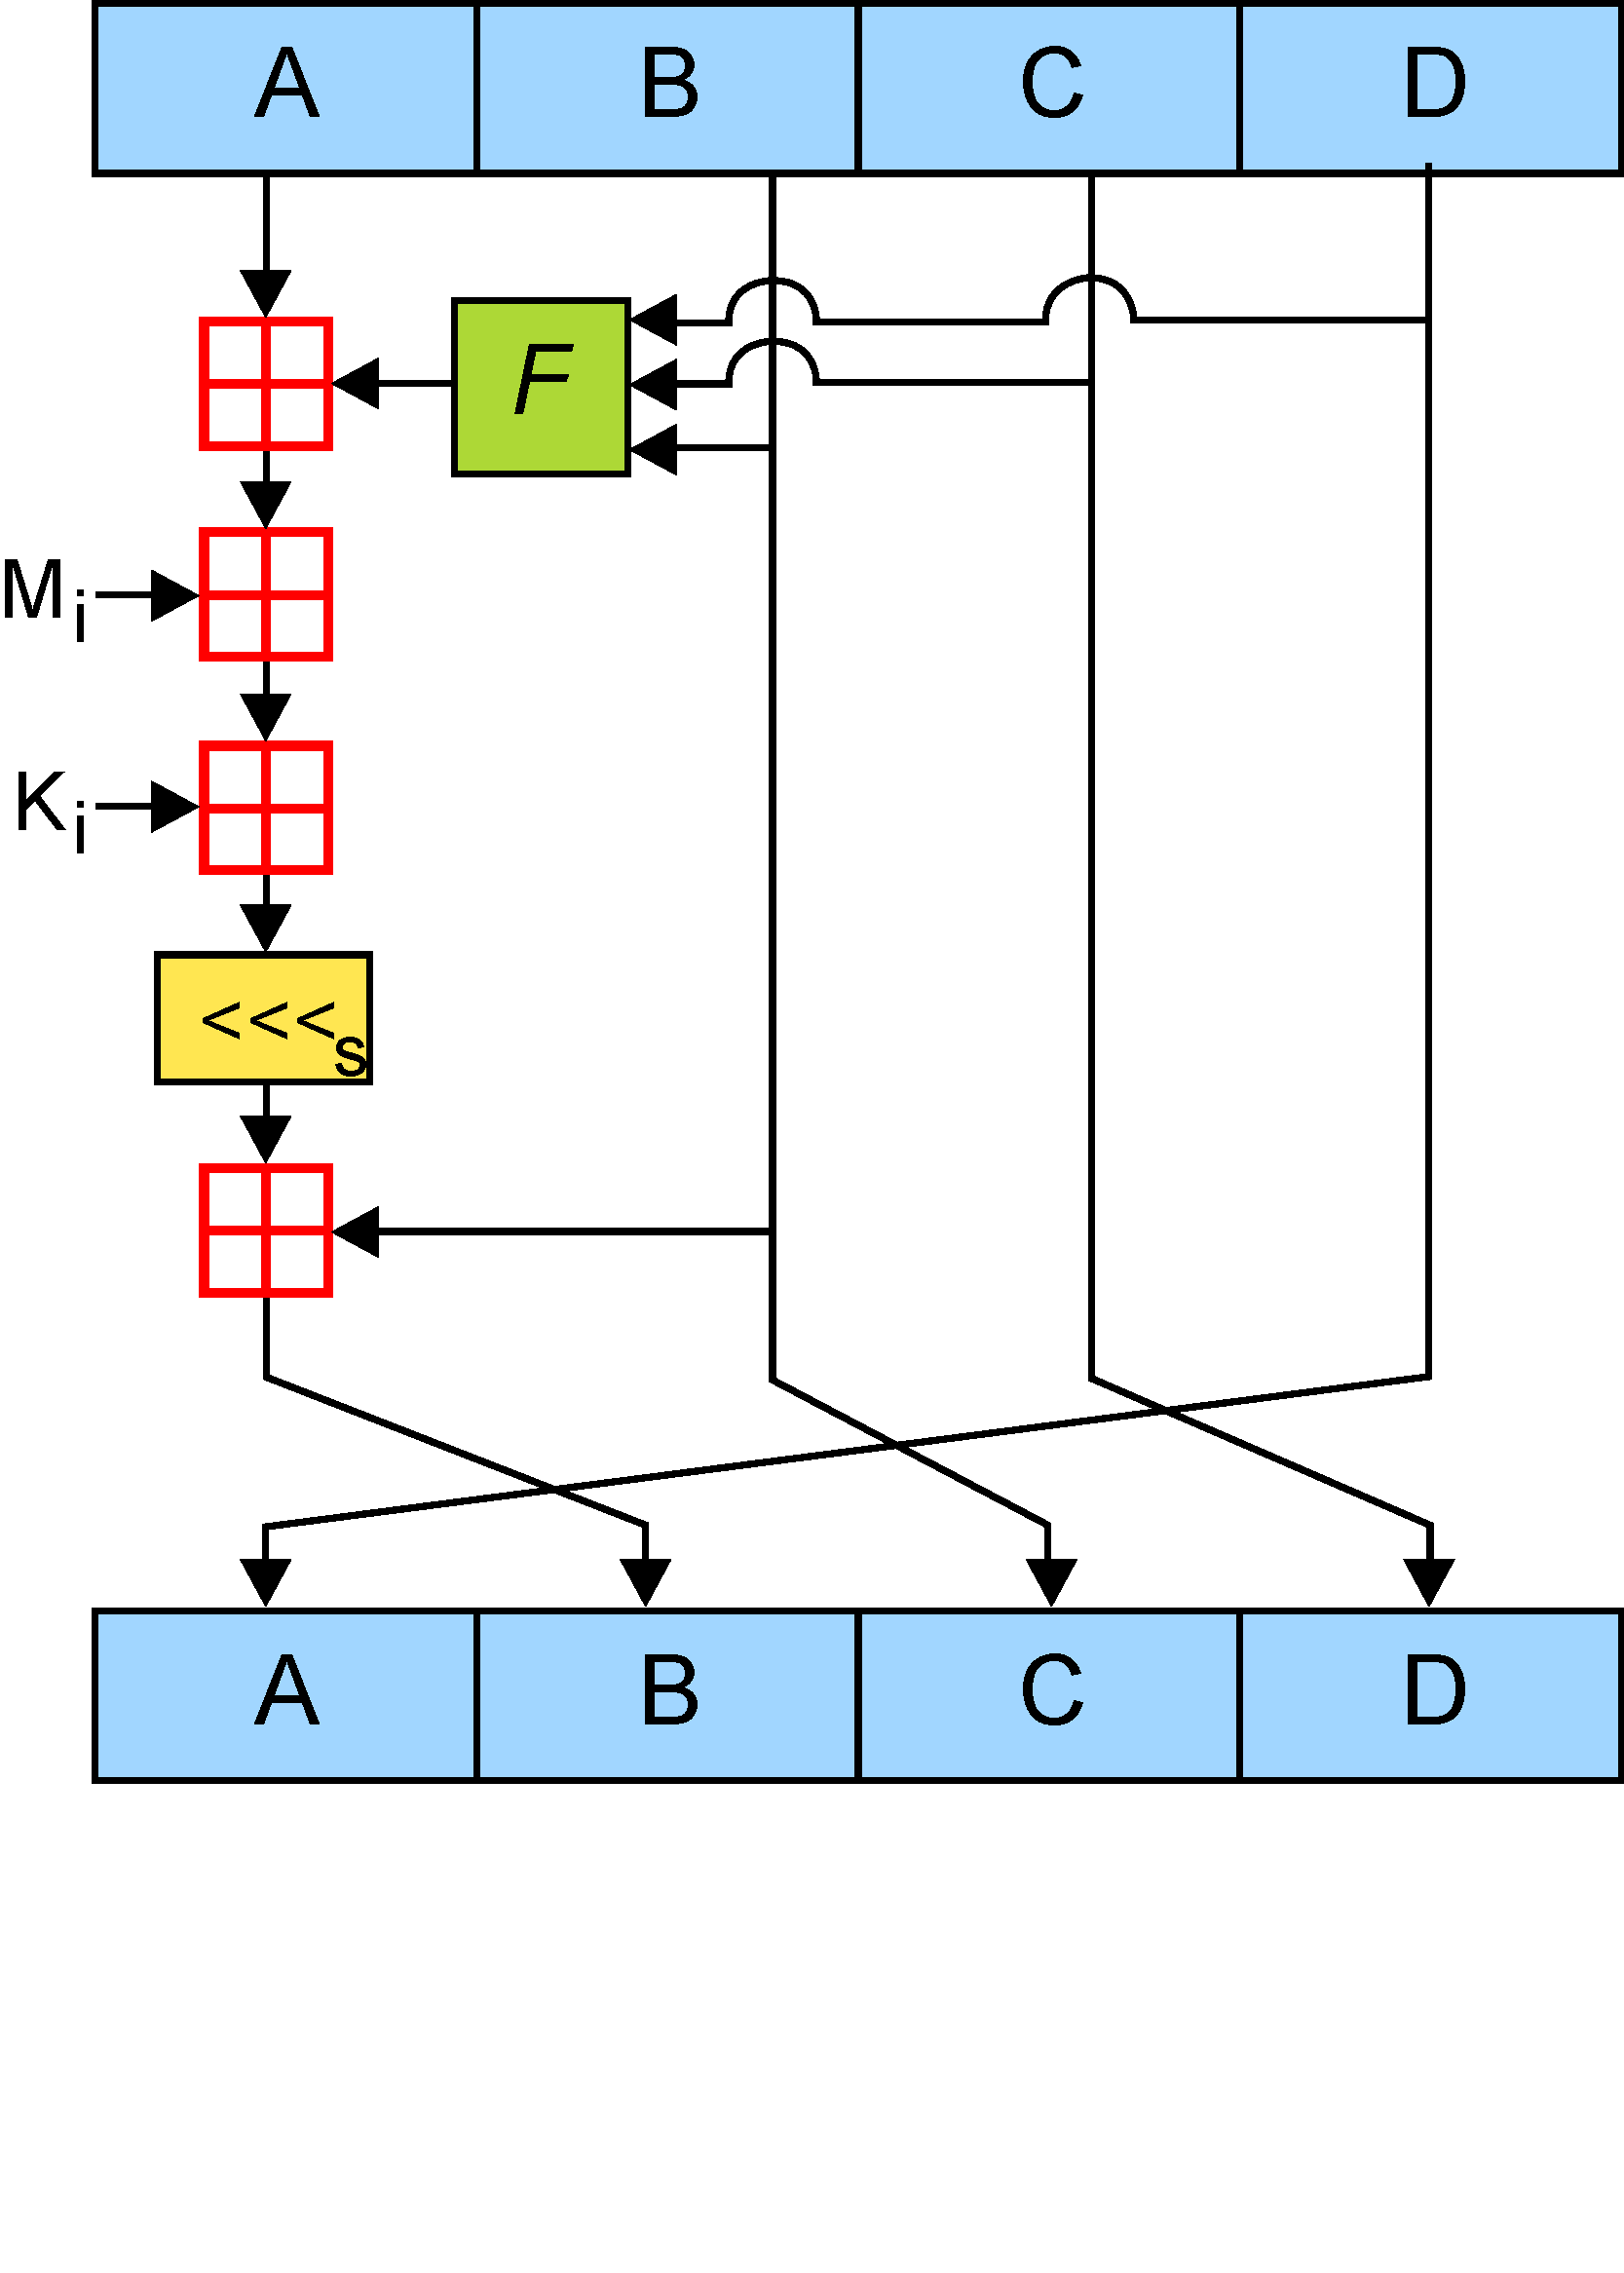
\includegraphics[width=0.6\textwidth]{images/sec-6/MD5/MD5}
    \caption[A single round of the MD5 hash algorithm]{A single round of the MD5
        hash algorithm. It consists of 64 iterations of this operation, split
        into 4 rounds of 16 iterations each. $F$ is a nonlinear function that is
        different for each round, $M_i$ denotes a 32-bit block of the input
        message, and $K_i$ a 32-bit constant. $\lll_s$ is left rotation by $s$
        bits, and $\boxplus$ addition modulo $2^{32}$. Image from
        \url{http://en.wikipedia.org/wiki/MD5}.}
    \label{fig:md5_round}
\end{figure}


\begin{lstlisting}[style=haskell_float
    ,label=lst:md5
    ,caption={A single round of the MD5 hash algorithm}]
type MD5        = (Word32, Word32, Word32, Word32)      -- output 128-bit digest
type Dictionary = Array DIM2 Word32                     -- input 16$\times$32-bit words per block

md5Round :: Acc Dictionary -> Exp DIM1 -> Exp MD5
md5Round dict (unindex1 -> word)
  = lift
  $ foldl step (a0,b0,c0,d0) [0..64]
  where
    step (a,b,c,d) i
      | i < 16    = shfl ((b .&. c) .|. ((complement b) .&. d))         -- F
      | i < 32    = shfl ((b .&. d) .|. (c .&. (complement d)))         -- G
      | i < 48    = shfl (b `xor` c `xor` d)                            -- H
      | i < 64    = shfl (c `xor` (b .|. (complement d)))               -- I
      | otherwise = (a+a0,b+b0,c+c0,d+d0)
      where
        shfl f = (d, b + ((a + f + k i + get i) `rotateL` r i), b, c)

    get :: Int -> Exp Word32
    get i
      | i < 16    = getWord32le i
      | i < 32    = getWord32le ((5*i + 1) `rem` 16)
      | i < 48    = getWord32le ((3*i + 5) `rem` 16)
      | otherwise = getWord32le ((7*i)     `rem` 16)

    getWord32le :: Int -> Exp Word32
    getWord32le (constant -> i) = dict ! index2 word i

    a0, b0, c0, d0 :: Exp Word32        -- initial values (constants)

    k :: Int -> Exp Word32              -- binary integer part of sines \& cosines (in radians)
    k i = constant (ks P.!! i)          -- (constants)
      where ks = [ ... ]

    r :: Int -> Exp Int                 -- per-round shift amounts
    r i = constant (rs P.!! i)          -- (constants)
      where rs = [ ... ]
\end{lstlisting}

The input to the @md5round@ function consists of a @(Z :. 16 :. n)@ input array
containing @n@ 512-bit input chunks to hash, which are processed by @n@ threads
in parallel. Note that the input array is stored in column major order, so that
accesses to the input @dict@ are coalesced. See \cite{NVIDIA:2012wf} for details
on CUDA memory access rules. In contrast, a CPU prefers the data to be laid out
in row-major order, so that the input chunk is read on a single cache line.
Exploring the differences in memory architectures between CPUs and GPUs, which
focus on task versus data parallelism respectively, is left for future work.

In the MD5 benchmark, each thread computes the hash of a 512-bit input column
and compares it to a supplied hash. If the values match, the input corresponds
to the plain text of the unknown hash. Table~\ref{tab:md5} compares Accelerate
to several other implementations. Note that the Hashcat program is not open
source and provides many additional options not supported by the Accelerate
implementation, so they are not strictly comparable. However, Hashcat is
regarded as the fastest password recovery tool available, so provides a useful
baseline.

\begin{table}
\centering
\small
\begin{tabu}{lr}
\toprule
\textbf{Benchmark} & \multicolumn{1}{c}{\textbf{Rate (GHash/sec)}} \\

\midrule
Accelerate      & \\
Repa (-N8)      & \\
Hashcat (CPU)   & \\
Hashcat (GPU)   & \\

\bottomrule
\end{tabu}
\caption{MD5 password recovery benchmarks}
\label{tab:md5}
\end{table}


\section{K-Means clustering}

In the $K$-means problem, the goal is to partition a set of observations into
$k$ clusters, in which each observation belongs to the cluster with the nearest
mean. Finding an optimal solution to the problem is NP-hard, however there exist
efficient heuristic algorithms that converge quickly to a local optimum, and in
practice give good results. The most well known heuristic technique is Lloyd's
algorithm, which finds a solution by iteratively improving on an initial guess.
The algorithm takes as a parameter the number of clusters, makes an initial
guess at the centre of each cluster, and proceeds as follows:
%
\begin{enumerate}
    \item Assign each point to the cluster to which it is closest. This yields
        the new set of clusters.

    \item Compute the centroid of each cluster.

    \item Repeat steps (1) and (2) until the cluster locations stabilise.
        Processing is also stopped after some chosen maximum number of
        iterations, as sometimes the algorithm does not converge.
\end{enumerate}
%
The initial guess can be constructed by randomly assigning each point in the
data set to a cluster and then finding the centroids of those clusters. The core
of the algorithm is shown in Listing~\ref{lst:kmeans}, which computes the new
cluster locations. To complete the algorithm, the function @makeNewClusters@ is
applied repeatedly until convergence, or some maximum iteration limit is
reached. While the algorithm works for any number of dimensions, the
implementation shown here is for two dimensional points only.

\begin{lstlisting}[style=haskell_float
    ,label=lst:kmeans
    ,caption={$K$-means clustering for 2D points}]
type Point a    = (a, a)
type Id         = Word32
type Cluster a  = (Id, (a, a))
type PointSum a = (Word32, (a, a))

distance :: (Elt a, IsNum a) => Exp (Point a) -> Exp (Point a) -> Exp a
distance u v = ...

findClosestCluster
    :: forall a. (Elt a, IsFloating a, RealFloat a)
    => Acc (Vector (Cluster a))
    -> Acc (Vector (Point a))
    -> Acc (Vector Id)
findClosestCluster clusters points =
  A.map (\p -> A.fst $ A.sfoldl (nearest p) z (constant Z) clusters) points
  where
    z = constant (-1, inf)

    nearest :: Exp (Point a) -> Exp (Id, a) -> Exp (Cluster a) -> Exp (Id, a)
    nearest p st c =
      let d  = A.snd st
          d' = distance p (centroidOfCluster c)
      in
      d' <* d ? ( lift (idOfCluster c, d') , st )

makeNewClusters
    :: forall a. (Elt a, IsFloating a, RealFloat a)
    => Acc (Vector (Point a))
    -> Acc (Vector (Cluster a))
    -> Acc (Vector (Cluster a))
makeNewClusters points clusters
  = pointSumToCluster
  . makePointSum
  . findClosestCluster clusters
  $ points
  where
    npts        = size points
    nclusters   = size clusters

    pointSumToCluster :: Acc (Vector (PointSum a)) -> Acc (Vector (Cluster a))
    pointSumToCluster ps =
      A.generate (A.shape ps)
                 (\ix -> lift (A.fromIntegral (unindex1 ix), average (ps ! ix)))

    makePointSum :: Acc (Vector Id) -> Acc (Vector (PointSum a))
    makePointSum = A.fold1 addPointSum . pointSum

    pointSum :: Acc (Vector Id) -> Acc (Array DIM2 (PointSum a))
    pointSum nearest =
      A.generate (lift (Z :. nclusters :. npts))
                 (\ix -> let Z:.i:.j = unlift ix    :: Z :. Exp Int :. Exp Int
                             near    = nearest ! index1 j
                             yes     = lift (constant 1, points ! index1 j)
                             no      = constant (0, (0,0))
                         in
                         near ==* A.fromIntegral i ? ( yes, no ))

    average :: Exp (PointSum a) -> Exp (Point a)
    average ps = ...            -- average of the $x$- and $y$-coordinates

    addPointSum :: Exp (PointSum a) -> Exp (PointSum a) -> Exp (PointSum a)
    addPointSum x y = ...       -- component-wise addition
\end{lstlisting}

Figure~\ref{fig:kmeans} compares the performance of the implementation shown
here to several other CPU implementations.

\section{Discussion}
% \subsection{Related Work}
% \subsection{Future Work}

% \begin{itemize}
%     \item performance \& analysis
%     \begin{itemize}
%       \item What is an optimisation? Describe the metrics considered.
%         \begin{itemize}
%           \item wall-clock time, parallel speedup??
%           \item instruction count
%           \item memory traffic (load/store/coalescing)
%           \item memory size (heap, register count, shared memory)
%           \item program size (number of parallel steps)
%           \item code size (generated binary, compilation time c.f. code complexity)
%         \end{itemize}
%     \end{itemize}
%
%     \item expressiveness / example programs
%     \item difficulties
%     \begin{itemize}
%         \item code generation
%         \item unintentional nesting
%     \end{itemize}
% \end{itemize}


%
% conclusions, related work, future work
%
%
% aim:
%   implement programming language targeting parallel hardware / GPUs
%
% why:
%   higher level of abstraction, still competitive with hand-written / lower
%   level programs.
%
% how:
%   (a) purely functional language of parallel array operations
%   (b) runtime code generationn
%   (c) runtime system for efficiently managing stuff
%   (d) sharing and fusion optimisations
%
% result:
%   * results show that we have achieved this for a range of benchmark programs.
%     significant future work will be the support expressing nested data
%     parallel programs.
%
%   * Some things remain difficult/impossible to express (general recursion,
%     nested parallelism) or are less efficient..?
%
% last: overall we can see that i should get a floopy hat


\chapter{Conclusion}
\label{ch:conclusion}

\epigraph{A new scientific truth does not triumph by convincing its opponents
and making them see the light, but rather because its opponents eventually die,
and a new generation grows up that is familiar with it.}%
{\textsc{---max planck}}

% \epigraph{The best way to predict the future is to implement it.}
% {\textsc{---david heinemeier hansson}}

% Purely functional programming is a good model for programming massively parallel
% SIMD processors such as graphics processing units. Indeed, all current GPU
% programming models, including CUDA, an imperative C-like programming language,
% implicitly emphasise a purely functional style for writing kernels, where global
% effects must be tightly controlled by the user. Indeed, functional programming
% may be \emph{the} main virtue of GPU programming, even if this fact is not
% widely recognised.

% Bubbabear worked thuuuuuuuuper hard to write the thesises. Pwease give him his
% doctor hat now pweaaaaaaaaaaaaaaaase~<3

The present dissertation argues that purely functional embedded languages
represent a good programming model for making effective use of  massively
parallel SIMD hardware. Indeed, all current GPU programming models, including
CUDA, implicitly emphasise a purely functional style, where global side-effects
must be tightly controlled by the user.

% Indeed, all current GPU programming models, including CUDA --- the standard,
% imperative, C-like programming language for NVIDIA GPUs --- implicitly emphasise
% a purely functional style of writing kernels, where global side-effects must be
% tightly controlled by the user.

To this end, this thesis has developed a purely functional language, compiler,
and runtime system for executing flat data-parallel array computations targeting
graphics processing units. When implementing such an embedded language, the
na\"ive compilation of such programs quickly leads to both code explosion and
excessive intermediate data structures. The resulting slowdown is not acceptable
on target hardware that is usually chosen to achieve high performance. This
thesis demonstrates that our embedding in Haskell, combined with the program
optimisations and runtime system that I have implemented in this thesis, are a
successful approach to implementing an expressive array programming language
targeting bulk-parallel SIMD hardware. Moreover, I demonstrate that the
Accelerate language and CUDA backend that I have developed simultaneously offers
a higher level of abstraction while often approaching the performance of
traditional low-level methods for programming GPUs.

Chapter~\ref{ch:accelerate} introduces Accelerate, an embedded language of
parameterised, collective array operations. Accelerate is our approach to
reducing the complexity of programming massively parallel multicore processors
such as GPUs. The choice of language operations is informed by the scan-vector
model, which has been shown to be suitable for a wide range of algorithms and
can be implemented efficiently on the GPU\@. We extend this model with
parameterised, rank-polymorphic operations over multidimensional arrays, making
Accelerate more expressive than previous high-level GPU programming language
proposals.

Chapter~\ref{ch:implementation} details how I implemented the Accelerate backend
which targets programmable graphics processing units. While the current
implementation targets CUDA, the same approach works for other target languages
such as OpenCL and LLVM. In the implementation of Accelerate's CUDA backend, I
regard the collective operations of the Accelerate language as algorithmic
skeletons, where a parallel program is composed of one or more parameterised
skeletons, or templates, encapsulating specific parallel behaviour. The
dynamically generated code is specialised to the capabilities of the current
hardware, and to minimise the overhead of online compilation, kernels are
compiled in parallel and asynchronously with other operations, and previously
compiled kernels are cached and reused. The runtime system automatically manages
data on the GPU, minimising allocations and data transfers and overlapping
host-to-device transfers with other operations. The execution engine optimises
kernel launches for the current hardware to maximise thread occupancy, and
kernels are scheduled so that independent operations are executed concurrently,
for devices that support this capability. All this and more is done to ensure
that the Accelerate runtime system executes programs as efficiently as possible.

Chapter~\ref{ch:optimising} describes our solution to what we found as the two
most pressing performance limitations for executing embedded array computations:
sharing recovery and array fusion. In particular, Chapter~\ref{ch:optimising}
discusses my novel approach to type-safe array fusion for compilers targeting
bulk-parallel SIMD hardware. Fusion for a massively data-parallel embedded
language instrumented via algorithmic skeletons requires a few uncommon
considerations compared to existing shortcut fusion methods. This problem was
tacked by classifying array operations into two categories: producers are
operations where individual elements are computed independently, while consumers
need to know exactly how the input elements depend on each other in order to
implement the operation efficiently in parallel. The problem with existing
fusion systems is that this information is obfuscated, and as a result the
parallel interpretation of the program is lost. Program fusion is realised in
two stages. First, sequences of producer operations are fused using
type-preserving source-to-source term rewrites. In the second stage, the fused
producer representation is embedded directly into the consumer skeleton during
code generation. This phase distinction is necessary in order to support the
different properties of producers and consumers.

Following these two main chapters, Chapter~\ref{ch:results} presents a series of
benchmarks comparing the performance of the Accelerate program to hand-optimised
reference implementations. The benchmarks illustrate the positive effect of the
optimisations discussed in this thesis, and the accompanying analyses discuss
future work that can be undertaken in cases where the performance of the
Accelerate program is lower than that of the reference solution. Overall, I have
demonstrated that the Accelerate language is suitable for expressing a wide
range of programs, and that the runtime system and program optimisations
described in this thesis result in programs that are often competitive with low
level, hand optimised solutions.


\section{Research contribution}

This thesis presents two main research contributions. First, it demonstrates how
to implement a high-performance embedded language and runtime system. Second, it
establishes a novel method of array fusion for languages targeting bulk-parallel
SIMD hardware. Together, these contributions provide an embedded language of
array operations, which achieves performance comparable to traditional
imperative language approaches, but at a much higher level of abstraction.

\subsection{A high-performance embedded language}

While the current generation of graphics processing units are massively parallel
processors with peak arithmetic and memory throughput rates much higher than
traditional CPUs, attaining the advertised $100\times$ speedups remains a work
intensive exercise that requires a substantial degree of expert knowledge.
Several researchers have attempted to ameliorate the status quo, by either using
a library to compose GPU code or by compiling a subset of a high-level language
to low-level GPU code. However, no other proposal has offered a high-level
interface with the breath and expressivity of operations as the Accelerate
language together with an implementation whose performance is comparable to
low-level programming languages.

% no other high-level embedded language has provided either
% the breath and expressivity of operations supported by Accelerate, nor the
% underlying runtime system necessary to achieve competitive performance.

The implementation of Accelerate's CUDA backend, covered in
Chapter~\ref{ch:implementation}, is original in that it successfully addresses
these problems. While the current implementation targets CUDA, my approach to
code generation works for other languages targeting data or control parallel
hardware, and the underlying runtime system is applicable to any deeply embedded
language which is implemented via runtime code generation and online
compilation.


\subsection{A fusion system for parallel array languages}

Although the topic of fusion has received significant prior attention,
particularly in the context functional programming languages, none of the
existing techniques are adequate for a type-preserving embedded language
compiler targeting massively parallel SIMD hardware such as graphics processing
units.

The implementation of fusion for embedded array languages implemented via
algorithmic skeletons, as developed in Chapter~\ref{ch:optimising}, is original.
In particular, because the fusion transformation retains the structure of the
program as a sequence of collective operations, our compilation techniques
developed in Chapter~\ref{ch:implementation} are able to generate efficient
parallel implementations of fused operations via skeleton template
instantiation. Our fused skeletons are able to exploit all levels of the
processor thread and memory hierarchy, which is of crucial importance to
achieving high performance.


% \section{Related work}
%
% Previous chapters have already covered related work of special relevance to the
% topics presented in their respective chapters. I refer readers to those
% chapters, and simply make some general remarks here.
%
% but I have nothing to say...


\section{Future work}

Based on the results of this thesis, a wide range of interesting future work is
possible. The previous chapters and the analysis of the benchmark results in
particular have already given suggestions for future work; these are not
repeated here, but some further topics are discussed.

\subsection{Nested data parallelism}

This thesis has demonstrated a high level array programming language and runtime
environment that is expressive and has performance competitive to much lower
level imperative program languages. However, the Accelerate language is
restricted to programs which express only \emph{flat} data parallelism, in which
the computation of each data element must itself be sequential. In practice,
this severely limits the applications of data-parallel computing, especially for
sparse and irregular problems~\cite{Prins:1999}.

Blelloch's pioneering work on NESL showed that it was possible to combine the
more flexible model of \emph{nested} data parallelism, where the computation of
each element may spawn further parallel computations, with a flat data parallel
execution model~\cite{Blelloch:1988iu}. Recent work has extend the flatting
transformation to support richer data types and higher order
functions~\cite{Jones:2008uu}.

Extending the Accelerate language to support the expression nested parallelism,
and implementing the vectorisation transformation to convert this nested
parallelism into a flat data parallel program which can be executed on the
compiler and runtime system presented in this thesis, is worthwhile future work.
This would allow Accelerate to support programs that are very difficult to
parallelise in a flat data parallel setting, such as the Barnes-Hut algorithm
for $N$-body simulation~\cite{Barnes:1986}.


\subsection{Type-preserving code generation}

The Accelerate language is richly typed, maintaining full type information of
the embedded language in the term tree and during the transformations described
in this thesis. Since Accelerate is an embedded language implemented via online
compilation, compilation time of the Accelerate program corresponds to Haskell
program \emph{runtime}. By encoding type information into the Accelerate terms
that are checked by the Haskell type checker at Haskell compile time, we ensure
that only well formed Accelerate programs will be compiled, reducing the number
of possible runtime errors.

Although we ensure the source program is well typed, the implementation of code
generation presented in this thesis does not reflect the types of the target
language into the Haskell type system. Thus, any errors in translating the
Accelerate program into CUDA source code will not be detected at Haskell
compilation time, and will instead raise a runtime error when the generated code
is compiled. Adding a fully type preserving compiler that translates the
well-typed Accelerate program into verifiable target code is important future
work.


\subsection{Flexibility in the optimisation pipeline}

Chapter~\ref{ch:results} demonstrated the positive effects of the optimisations
that have been presented in this thesis. However, the optimisation pipeline is
completely fixed, so changing or extending the set of optimisations requires
changing the compiler itself.

Useful future work would be the ability to control the existing optimisation
process, for example by specifying the eagerness with which producer operations
should be fused. This would allow the user to override the default behaviour of
always fusing expressions that are used exactly once in subsequent computations.

Orthogonal to this work would be the ability to extend the optimisation process
through the implementation of a system of extensible rewrite
rules~\cite{Jones:2001wm}. Although our host language Haskell compiler supports
rewrite rules, since Accelerate programs can be generated at program runtime, we
require rewrite rules at program runtime as well. In addition to allowing the
compiler to generate rules internally to propagate information obtained from
automated analyses, this would allow library authors to express domain specific
knowledge that the compiler can not discover for itself. For example, the author
of a library of linear algebra routines might like to express the equivalence
that $x^{-1}x \mapsto 1$, or the less obvious $\left( 1 - x y \right)^{1}x
\mapsto x \left( 1 - y x \right)^{-1}$. While a programmer may be unlikely to
write such expressions themselves, they can easily appear when aggressive
inlining brings together code that was written separately. Adding the ability to
add rewrite rules to the program could be a very powerful feature, but raises
questions such as verifying whether the programmer-specified rules are
consistent with the underlying function definitions that they purport to
describe, or that the set of rules are confluent or even terminating.


% \begin{itemize}
% \item conclusion / summary discussion (2 days)
%
% \item future work
%     \begin{itemize}
%     \item frontend
%         \begin{itemize}
%             \item fusion cost analysis (1 day)
%             \item user controllable fusion (e.g. inline/noinline annotations) (1 day)
%             \item used definable rewrite rules (1 day)
%         \end{itemize}
%     \item backend
%         \begin{itemize}
%             \item type-preserving code generation (1 day)
%         \end{itemize}
%     \item language
%         \begin{itemize}
%             \item first order flattening: naturally nested algorithms
%                 (barns-hutt) as well as convenience of expression
%                 (matrix-vector) (2 days)
%         \end{itemize}
%     \end{itemize}
% \end{itemize}



% BACK MATTER
% ~~~~~~~~~~~

\cleardoublepage
\stopthumb
\
\backmatter
\let\chapter\oldchapter
\fancyhead[ER]{}
\fancyhead[OL]{}

\cleardoublepage
\phantomsection
\addcontentsline{toc}{chapter}{Bibliography}
\bibliography{thesis}

\cleardoublepage
\phantomsection
\addcontentsline{toc}{chapter}{Index}
\printindex\markboth{Index}{Index}

\end{document}

